 \documentclass[12pt, sfheadings, oneside, noindentfirst]{mwbk}

\usepackage[utf8]{inputenc}
\usepackage{polski}

\usepackage[T1]{fontenc}
\usepackage{lmodern}
\usepackage[scaled=0.8]{beramono}

\usepackage{graphicx}
\graphicspath{ {./images/} }

\usepackage{hyperref}
\usepackage{pdfpages}
\usepackage{makeidx}
\makeindex

\usepackage{newunicodechar}
\newunicodechar{→}{{\tiny$\rightarrow$\normalsize}}
%~\newunicodechar{←}{$\leftarrow$}
\newunicodechar{“}{``}
\newunicodechar{”}{''}
\newunicodechar{’}{'}
\newunicodechar{π}{$\pi$}
\newunicodechar{½}{$\frac{1}{2}$}
\newunicodechar{⅓}{$\frac{1}{3}$}
\newunicodechar{¼}{$\frac{1}{4}$}
\newunicodechar{…}{\ldots}
\newunicodechar{×}{$\times$}
\newunicodechar{ϕ}{$\varphi$}
\newunicodechar{≈}{$\approx$}
\newunicodechar{―}{---}

\pagestyle{plain} 

\begin{document}
\author{Marijn Haverbeke}
\title{\Huge JavaScript. I wszystko jasne \\ \large Nowoczesne wprowadzenie do programowania}

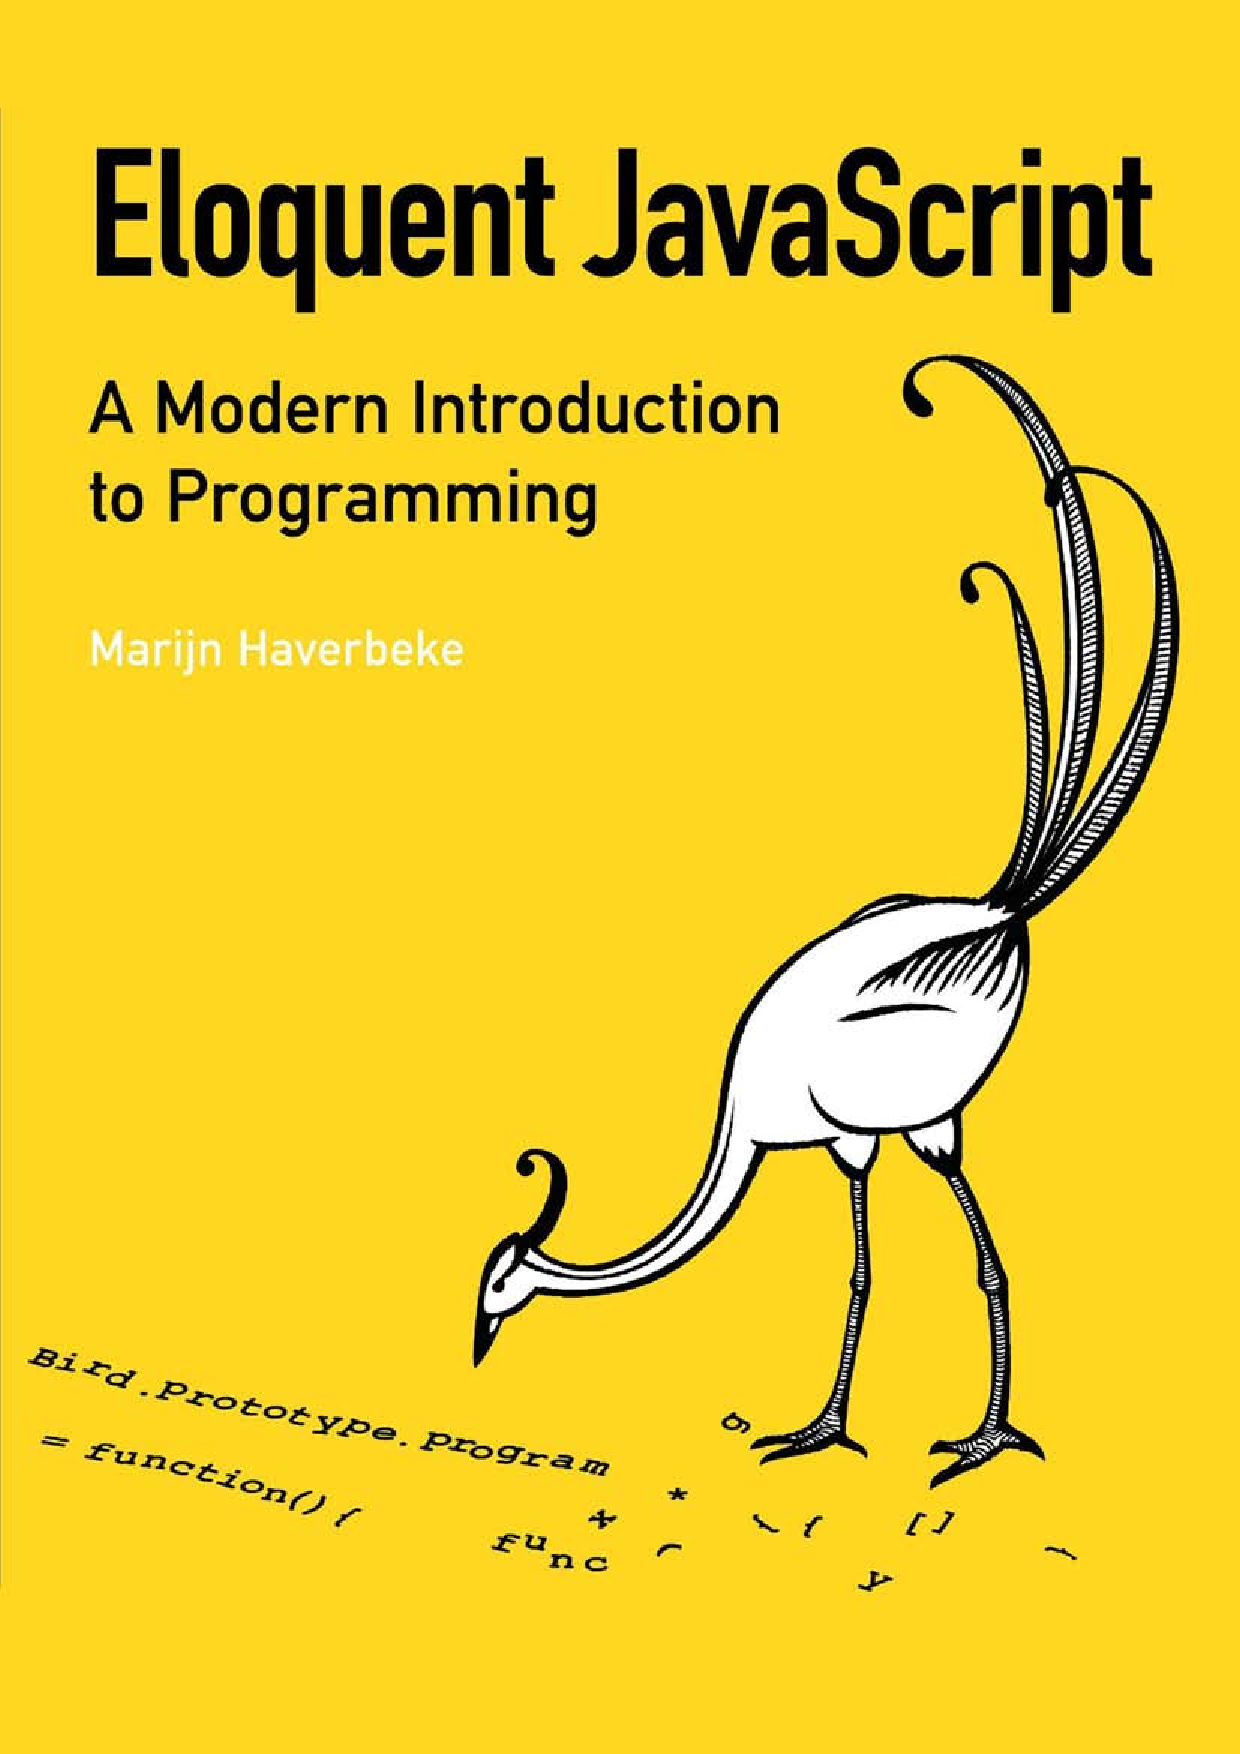
\includepdf[pages=1]{cover.pdf}

\maketitle

\setcounter{page}{2}

\noindent Tytuł oryginału: \emph{Eloquent JavaScript. A Modern Introduction to Programming}

\bigskip

\noindent Tłumaczenie: Łukasz Piwko

\bigskip

\noindent \noindent Copyright \textcopyright{} Marijn Haverbeke

\bigskip

Autorem tej książki jest Marijn Haverbeke \texttt{\href{mailto:marijnh@gmail.com}{<marijnh@gmail.com>}}. Powstała ona w oryginale w wersji cyfrowej, zawierającej interaktywne przykłady kodu i jest dostępna na stronie \texttt{\href{http://eloquentjavascript.net/1st\_edition/}{eloquentjavascript.net/1st\_edition/}}. Istnieje również drugie wydanie które jest dostępne zarówno w formie elektronicznej (\url{http://eloquentjavascript.net}) jak i w wersji papierowej. Wersję papierową można kupić w sklepie \href{http://www.amazon.com/gp/product/1593275846/}{Amazon}.

Polskie tłumaczenie pod tytułem \emph{JavaScript. I wszystko jasne. Nowoczesne wprowadzenie do programowania}  zostało udostępnione w serwisie Shebang (\url{http://shebang.pl/kursy/wszystko-jasne/}) 16 stycznia 2013.

Użyto na licencji Creative Commons Uznanie autorstwa 3.0 Unported (\texttt{\href{http://creativecommons.org/licenses/by/3.0/deed.pl}{http://creativecommons.org/licenses/by/3.0/}}).

\setcounter{tocdepth}{0}
\tableofcontents
\setcounter{tocdepth}{2}

\chapter{Wprowadzenie do języka JavaScript}
\label{chap:1}

Większość pierwszych komputerów była wyposażona w jeden język programowania, najczęściej jakąś wersję Basic-a\index{Basic}. Współpraca z komputerem wymagała posługiwania się tym językiem, przez co każdy użytkownik komputera, czy tego chciał czy nie, musiał się go nauczyć. Obecnie komputery można spotkać wszędzie, a typowy użytkownik potrafi tylko klikać myszą w odpowiednich miejscach. Większości osób to wystarcza. Jednak dla wielu z nas, osób lubiących poszperać w urządzeniach, usunięcie języka programowania z~codziennego użytkowania komputera jest niekorzystne.

  
Na szczęście dzięki postępowi, jaki dokonał się w sieci WWW, każdy komputer ma pewne środowisko programistyczne. Jest to przeglądarka internetowa obsługująca \textbf{JavaScript}. Ze względu na aktualnie przyjęte zwyczaje polegające na ukrywaniu przed użytkownikiem kwestii technicznych, środowisko to jest dobrze ukryte, ale można się do niego dostać poprzez okno przeglądarki i wykorzystać do nauki programowania.

  
Taki był też cel napisania tej książki.


\begin{center}
• • • • •
\end{center}

  
\begin{quotation}
Nie oświecę tych, którzy nie chcą się uczyć, ani nie rozbudzę pasji w~tych, którzy nie są skłonni samodzielnie szukać rozwiązań. Jeśli podam im jeden róg kwadratu, a oni nie podadzą mi pozostałych trzech, to nie ma sensu powtarzać wszystkiego od nowa 
    
    ― Konfucjusz
\end{quotation}
  
Oprócz bycia wprowadzeniem do JavaScriptu, książka ta ma aspiracje służyć jako wstępny kurs zasad programowania w~ogóle. Okazuje się, że programowanie jest trudne. Podstawowe zasady programowania są wprawdzie jasne i proste. Ale programy zbudowane wg tych zasad są zazwyczaj na tyle skomplikowane, że rządzą się swoimi prawami. Z tego powodu programowanie rzadko kiedy jest łatwe i przewidywalne. Jak powiedział uznawany za ojca tej dziedziny Donald Knuth, programowanie to \emph{sztuka}.

  
Aby maksymalnie wykorzystać treść tej książki, nie można poprzestać tylko na jej biernym przeczytaniu. Staraj się być cały czas skoncentrowany, rozwiązuj zadania i do kolejnych partii materiału przechodź wyłącznie wtedy, gdy masz poczucie, że dobrze rozumiesz kwestie omówione do tej pory.


\begin{center}
• • • • •
\end{center}

  
\begin{quotation}
Programista komputerowy tworzy odrębne wszechświaty, za które ponosi wyłączną odpowiedzialność. W postaci programów można tworzyć wszechświaty o praktycznie nieskończonym stopniu złożoności.
    
    ― Joseph Weizenbaum, \emph{Computer Power and Human Reason}
\end{quotation}
  
Program komputerowy jest wieloma rzeczami na raz. Jest to tekst napisany przez programistę, jest to siła sterująca działaniem komputera, jest to porcja danych w pamięci komputera, mimo że steruje działaniami wykonywanymi na tej samej pamięci. Analogie, w których próbuje się porównywać programy do obiektów świata realnego są zazwyczaj nietrafione, ale jedna, porównująca komputer do maszyny, trochę pasuje. Tryby zegarka na rękę są do siebie dopasowane z wielką precyzją i jeśli zegarmistrz dobrze się spisze, taki zegarek będzie dokładnie pokazywał godzinę. Podobnie elementy programu muszą być do siebie precyzyjnie dopasowane i jeśli programista zna się na swojej pracy, to jego program będzie działał bezawaryjnie.

  
Komputer jest maszyną stanowiącą środowisko pracy tych niematerialnych maszyn. Komputery same w sobie potrafią wykonywać tylko absurdalnie proste działania. Jedyny powód, dla którego są przydatne jest taki, że to co robią wykonują nieprawdopodobnie szybko. Jeśli sprytnie wykorzysta się tę zdolność komputerów do wykonywania prostych czynności i odpowiednio się je zmiesza, to można uzyskać bardzo skomplikowane efekty.

  
Dla niektórych pisanie programów komputerowych to niezwykła zabawa. Program to budowla wzniesiona z myśli. Jego utworzenie nic nie kosztuje, nic on nie waży i szybko rośnie pod wprawnymi palcami programisty. Jeśli damy się ponieść, program może nam się rozrosnąć i stać się skomplikowany do tego stopnia, że nawet ten, kto go napisał będzie miał problem ze zrozumieniem jak działa. Jest to jeden z największych problemów dotyczących programowania. Dlatego właśnie tak wiele używanych obecnie programów często ulega awariom.

  
Program gdy działa jest piękny. Sztuka programowania to umiejętność radzenia sobie ze złożonością problemów. Dobry program jest zwięzły i maksymalnie prosty w swojej złożoności.


\begin{center}
• • • • •
\end{center}

  
Wielu programistów uważa obecnie, że z tą złożonością najlepiej jest radzić sobie używając do pisania programu tylko kilku dobrze poznanych technik. Sformułowano ścisłe reguły określające, jak powinny wyglądać programy, a ci którzy ośmielą się je złamać zostaną przez zawistnych okrzyknięci \emph{złymi} programistami.

  
Co za barbarzyństwo wobec bogactwa technik programistycznych! W imię redukowania go do prostego i przewidywalnego rzemiosła wszystkie dziwne i~piękne programy zostały skazane na banicję. Różnorodność technik programistycznych jest oszałamiająca i wciąż wiele pozostaje do odkrycia. Oczywiście trzeba uważać na rozmaite pułapki, przez które niedoświadczony programista może popełnić wiele strasznych błędów, ale to oznacza tylko tyle, że należy postępować ostrożnie i cały czas mieć oczy szeroko otwarte. Podczas nauki ciągle będziesz odkrywać coraz to nowsze obszary do zbadania i kolejne wyzwania, z którymi można się zmierzyć. Programista niechcący się kształcić jest skazany na stagnację, utratę radości z programowania oraz wypalenie zawodowe (i w efekcie zostanie menedżerem).

  
Jeśli o mnie chodzi, najważniejszym kryterium oceny programu jest to, czy jest poprawny. Oczywiście wydajność, przejrzystość i rozmiar również mają znaczenie, ale znalezienie kompromisu między tymi trzema czynnikami jest indywidualną kwestią dla każdego programisty. Podstawowe zasady są przydatne, ale nie należy bać się ich łamać.


\begin{center}
• • • • •
\end{center}

  
Na początku ery komputerów w ogóle nie było języków programowania. Kod programów wyglądał mniej więcej tak:

  
\begin{verbatim} 
00110001 00000000 00000000
00110001 00000001 00000001
00110011 00000001 00000010
01010001 00001011 00000010
00100010 00000010 00001000
01000011 00000001 00000000
01000001 00000001 00000001
00010000 00000010 00000000
01100010 00000000 00000000
 \end{verbatim}
  
Ten program sumuje liczby od 1 do 10, a następnie drukuje wynik ($1 + 2 + … + 10 = 55$). Można go uruchomić na bardzo prostym komputerze. Programowanie pierwszych komputerów polegało na przełączaniu wielkich tablic przełączników lub robieniu dziur w kartonie, który następnie wprowadzało się do komputera. Nietrudno sobie wyobrazić, jak żmudna i zagrożona możliwością popełnienia błędu była to praca. Napisanie nawet prostego programu wymagało dużej inteligencji i dyscypliny, a napisanie skomplikowanego programu graniczyło z niemożliwością.

  
Oczywiście programista wprowadzając do komputera te tajemniczo wyglądające wzory bitów (tak nazywają się przedstawione powyżej zera i jedynki) czuł się jak jakiś potężny czarownik. To na pewno dawało ogromne poczucie satysfakcji z wykonywanej pracy.

  
Każdy wiersz programu zawiera jedną instrukcję. Po polsku można by było go napisać tak:

  \begin{enumerate}
    \item Zapisz liczbę 0 w komórce pamięci o numerze 0
    \item Zapisz liczbę 1 w komórce pamięci o numerze 1
    \item Zapisz wartość komórki pamięci nr 1 w komórce pamięci nr 2
    \item Zmniejsz wartość znajdującą się w komórce pamięci 2 o 11
    \item Jeśli wartość znajdująca się w komórce pamięci nr 2 to 0, przejdź do instrukcji 9
    \item Zwiększ wartość znajdującą się w komórce pamięci 0 o wartość znajdującą się w komórce pamięci nr 1
    \item Zwiększ wartość znajdującą się w komórce pamięci nr 1 o 1
    \item Przejdź do instrukcji 3
    \item Wyślij na wyjście wartość komórki pamięci nr 0
  \end{enumerate}
  
Podczas gdy ten tekst jest o wiele łatwiejszy do zrozumienia niż gmatwanina bitów, to jednak również niezbyt dobrze się go czyta. Sytuację można trochę poprawić, gdyby zamiast numerów instrukcji i komórek pamięci używać różnych nazw:

  
\begin{verbatim} 
 Ustaw 'suma' na 0
 Ustaw 'liczba' na 1
[pętla]
 Ustaw 'porównaj' na 'liczba'
 Odejmij 11 od 'porównaj'
 Jeśli 'porównaj' wynosi zero, przejdź do [koniec]
 Dodaj 'liczba' do 'suma'
 Dodaj 1 do 'liczba'
 Przejdź do [pętla]
[koniec]
 Zwróć 'suma'
 \end{verbatim}
  
Teraz łatwo jest dostrzec, w jaki sposób działa program. Widzisz to? W~dwóch pierwszych wierszach zostały przypisane początkowe wartości dwóm komórkom pamięci: \texttt{suma} będzie służyła do akumulowania wyniku programu, a \texttt{liczba} pozwoli nam śledzić, którą liczbą w danym momencie się zajmujemy. Najdziwniejsze pewnie są wiersze zawierające słowo \texttt{porównaj}. Program „chce” sprawdzić czy \texttt{liczba} jest równa 11, aby dowiedzieć się, czy ma już zakończyć działanie. Maszyna jest tak prymitywna, że może tylko sprawdzać, czy dana liczba jest zerem i na podstawie wyniku tego testu może podjąć decyzję (dokonać przeskoku). Dlatego komórka pamięci oznaczona jako \texttt{porównaj} jest używana do wykonania działania \texttt{liczba - 11}, od którego wyniku zależy dalsze działanie programu. Następne dwa wiersze dodają wartość \texttt{liczba} do wyniku i zwiększają \texttt{liczba} o jeden za każdym razem, gdy program obliczy, że nie jest to jeszcze 11.

  
Poniżej znajduje się ten sam program wyrażony w języku JavaScript:

  
  
\begin{verbatim} 
var total = 0, count = 1;
while (count <= 10) {
  total += count;
  count += 1;
}
print(total);
// → 55
\end{verbatim}
  
  
W kodzie tym widzimy kilka dalszych ulepszeń. Do najważniejszych można zaliczyć to, że niepotrzebne stały się instrukcje skoku w tę i z powrotem. Dba za nas o to magiczne słowo \texttt{while}. Powoduje ono wykonywanie kodu znajdującego się pod nim tak długo, jak długo spełniony jest jego warunek: \texttt{count <= 10}, który oznacza „\texttt{count} ma wartość mniejszą lub równą \texttt{10}”. Nie trzeba już tworzyć tymczasowej wartości i porównywać jej z zerem. To był mały głupi szczegół, ale właśnie jedną z zalet języków programowania jest to, że przejmują od nas konieczność pamiętania o tych błahostkach.

  
W końcu poniżej możesz zobaczyć, jak ten program mógłby wyglądać, gdyby można było używać wygodnych operatorów \texttt{range} i \texttt{sum}, które odpowiednio tworzyłyby zbiór liczb z określonego przedziału i obliczały sumę liczb w takim zbiorze:

  
\begin{verbatim} 
print(sum(range(1, 10)));
// → 55
\end{verbatim}
  
Morał z tej opowieści jest taki, że każdy program można zapisać na wiele sposobów, przy użyciu dużej i małej liczby wierszy kodu jak również czytelnie i nieczytelnie. Pierwsza wersja była kompletnie nieczytelna, natomiast ostatnia wygląda prawie jak zdania po angielsku. \texttt{print} the \texttt{sum} of the \texttt{range} of numbers from \texttt{1} to \texttt{10}. (w dalszych rozdziałach dowiesz się, jak tworzyć konstrukcje podobne do opisywanych tu operatorów \texttt{sum} i \texttt{range}.)

  
Dobry język programowania to taki, który pomaga programiście w pracy, umożliwiając mu wyrażanie myśli w bardziej abstrakcyjny sposób. Ukrywa nieistotne szczegóły, udostępnia wygodne w użyciu składniki (takie, jak konstrukcja \texttt{while}) oraz zwykle umożliwia programiście dodawanie własnych składników (takich, jak np. operacje \texttt{sum} i \texttt{range}).


\begin{center}
• • • • •
\end{center}

  
Aktualnie język JavaScript jest najczęściej używany zarówno w sposób inteligentny jak i straszny do robienia różnych rzeczy ze stronami internetowymi. \href{http://steve-yegge.blogspot.com/2007/02/next-big-language.html}{Niektórzy} twierdzą, że kolejna wersja języka JavaScript odegra ważną rolę także w innych dziedzinach. Nie jestem przekonany, czy tak będzie, ale jeśli interesujesz się programowaniem, to JavaScript bez wątpienia jest jednym z języków, które warto znać. Nawet jeśli nie będziesz zbyt często programował stron internetowych, wymagające gimnastyki umysłu przykłady, które pokażę Ci w tej książce zapadną Ci w pamięć, będą Ci się przypominać i~wywrą wpływ na Twoje przyszłe programowanie w innych językach.

  
Zapewne spotkasz też ludzi mówiących \emph{straszne} rzeczy o JavaScripcie. Wiele z tego, co mówią jest prawdą. Gdy po raz pierwszy poproszono mnie o napisanie czegoś w języku JavaScript, szybko znienawidziłem ten język. Prawie wszystko, co napisałem przechodziło bez błędów przez interpreter, ale działało kompletnie inaczej, niż chciałem. To oczywiście miało związek z tym, że nie miałem pojęcia, co robię, ale istnieje też realny problem: JavaScript jest absurdalnie liberalnym językiem. Zamierzeniem twórcy tego języka było sprawienie, aby był on jak najłatwiejszy w użyciu dla początkujących programistów. Jednak w rzeczywistości to tylko utrudnia znajdowanie problemów w programach, ponieważ system ich nie pokazuje.

  
Jednak elastyczność języka jest również jego zaletą. Można w nim korzystać z wielu technik, których nie można by było zastosować w bardziej sztywnych językach. Gdy nauczyłem się zasad JavaScriptu i trochę z nim popracowałem, na powrót go \emph{polubiłem}.


\begin{center}
• • • • •
\end{center}

  
Mimo swojej nazwy, język JavaScript ma niewiele wspólnego z językiem Java. Zbieżność ta jest wynikiem marketingowych zabiegów i nie powstała w~wyniku racjonalnego wyboru. W 1995 r., gdy firma Netscape opublikowała JavaScript, języka Java był intensywnie promowany i zdobywał ogromną popularność. Ktoś widocznie doszedł do wniosku, że może uda się zgarnąć także dla siebie kawałek tego marketingowego tortu. W ten sposób powstała ta nazwa.

  
Krewnym JavaScriptu jest coś, co nazywa się \textbf{ECMAScript}. Gdy obsługę JavaScriptu (lub czegoś podobnego) wprowadzono także w innych przeglądarkach niż Netscape, sporządzono dokument zawierający opis, jak dokładnie ten język powinien działać. Język, który w nim opisano został nazwany ECMAScript, po nazwie organizacji standaryzacyjnej, która zajęła się napisaniem tego standardu.

  
Standard ECMAScript opisuje język programowania ogólnego przeznaczenia i nie ma w nim ani słowa o jego integracji z jakąkolwiek przeglądarką internetową. W związku z tym JavaScript to ECMAScript plus dodatkowe narzędzia do manipulowania stronami internetowymi i oknami przeglądarki.

  
Język opisany w dokumencie standaryzacyjnym ECMAScript jest używany także w kilku innych technologiach. Do najważniejszych zalicza się Flash, w którym używany jest język ActionScript oparty na ECMAScript (chociaż nie jest on ściśle zgodny ze standardem). Flash to technologia umożliwiająca wstawianie na strony internetowe komponentów, które dużo się ruszają i robią mnóstwo hałasu. Zatem znajomość JavaScriptu nie zaszkodzi, jeśli kiedyś zechcesz utworzyć animację Flash.

  
JavaScript wciąż ewoluuje. Od czasu napisania tej książki ukazał się ECMAScript 5, który jest zgodny z wersją opisywaną w tej publikacji, ale zawiera już część funkcji, które my będziemy pisać samodzielnie. W najnowszych przeglądarkach obsługiwana jest ta najnowsza wersja JavaScriptu. W 2011 r. rozpoczęto prace nad standaryzowaniem „ECMAScript harmony”, bardziej radykalnego rozszerzenia języka. Nie obawiaj się, że któraś z tych nowych wersji sprawi, że informacje zawarte w tej książce staną się przestarzałe. Będą to rozszerzenia istniejącego języka, a więc prawie wszystko, co jest tu napisane będzie nadal aktualne.


\begin{center}
• • • • •
\end{center}

  
W większości rozdziałów w tej książce znajduje się dużo kodu źródłowego\footnote{Kod jest esencją każdego programu. Każdy fragment aplikacji, niezależnie jak długi, można nazwać używając tego słowa.}. Z doświadczenia wiem, że pisanie kodu w trakcie czytania jest bardzo ważnym czynnikiem pomagającym w nauce. Postaraj się nie tylko przejrzeć wszystkie przykłady, ale dokładnie je przestudiować i zrozumieć. Początkowo mogą wydawać Ci się trudne i niejasne, ale szybko zaczniesz wszystko rozumieć. To samo dotyczy ćwiczeń. Nie zakładaj, że je rozumiesz dopóki nie napiszesz rozwiązania, które będzie działać.

  
Dzięki temu, że kod źródłowy każdej strony internetowej można bez problemu podejrzeć, zawsze możesz zobaczyć, jak wyglądają programy JavaScript napisane przez innych. W ten sposób można sporo się nauczyć. Ponieważ większość programistów stron internetowych nie jest „profesjonalnymi programistami” albo uważa programowanie w języku JavaScript za mało interesujące zajęcie, mało który z nich solidnie nauczył się posługiwać tym językiem, przez co można znaleźć mnóstwo \emph{bardzo} niskiej jakości kodu. Jeśli będziesz zgłębiać tajniki programowania korzystając z brzydkich i niepoprawnych przykładów kodu, sam zaczniesz pisać taki sam kod. Dlatego uważaj, od kogo uczysz się programować.


\begin{center}
• • • • •
\end{center}

  
Aby ułatwić Ci wypróbowanie programów, została dodana specjalna konsola\index{konsola}, w której możesz przetestować zarówno przykładowe jak i własne programy. Jeśli używasz nowoczesnej przeglądarki (Internet Explorer od wersji 6, Firefox od wersji 1.5, Opera od wersji 9, Safari od wersji 3 lub Chrome), to na dole okna na każdej ze stron znajdziesz zielonkawy pasek. Aby otworzyć konsolę, należy kliknąć strzałkę znajdującą się po prawej stronie tego paska. (Podkreślam, że nie jest tu mowa o wbudowanej konsoli przeglądarki.)

  
Konsola ta zawiera trzy ważne elementy. Pierwszym z nich jest okno wyjściowe, w którym przedstawiane są wyniki działania programów i ewentualnie powiadomienia o błędach. Pod nim znajduje się pole tekstowe, w którym można wpisać kod JavaScript. Wpisz tam jakąś liczbę i naciśnij klawisz Enter, aby wykonać ten program. Jeśli kod wprowadzony w tym polu spowoduje wytworzenie jakiegoś sensownego wyniku, zostanie on wyświetlony w oknie wyjściowym. Teraz wpisz słowo \texttt{Źle!} i znowu naciśnij klawisz Enter. W oknie wyjściowym zostanie wyświetlone powiadomienie o błędzie. Za pomocą strzałek do góry i w dół można przechodzić do poprzednich i następnych poleceń.

  
Jeśli masz dłuższy fragment kodu, który zajmuje kilka wierszy i który chciałbyś przechować przez jakiś czas, to możesz użyć pola znajdującego się po prawej stronie. Do uruchamiania programów wpisanych w tym polu służy przycisk Wykonaj. Jednocześnie może być otwartych kilka programów. Aby otworzyć nowy pusty bufor, kliknij przycisk Nowy. Gdy otwartych jest kilka buforów, można je wybierać z menu rozwijanego znajdującego się obok przycisku Wykonaj. Przycisk Zamknij, jak się zapewne spodziewasz zamyka bufor.

  
W prawym górnym rogu każdego przykładowego programu znajduje się niewielki przycisk ze strzałką, który służy do uruchomienia tego programu. Przedstawiony wcześniej przykład wyglądał tak:

  
\begin{verbatim} 
var total = 0, count = 1;
while (count <= 10) {
  total += count;
  count += 1;
}
print(total);
 \end{verbatim}
  
Aby go wykonać, kliknij strzałkę. Przed strzałką znajduje się jeszcze inny przycisk, który służy do ładowania programu do konsoli. Po załadowaniu programu możesz go do woli modyfikować, aby zobaczyć, co się stanie. W~najgorszym przypadku utworzysz nieskończoną pętlę. Nieskończona pętla to taka konstrukcja, w której warunek instrukcji \texttt{while} nigdy nie zostaje spełniony. Pętla taka powstałaby na przykład, gdyby do zmiennej count zamiast \texttt{1} dodano \texttt{0}. Jeśli to zrobisz, program będzie działać w nieskończoność.

  
Na szczęście przeglądarki interesują się tym, co robią działające w nich programy. Gdy któryś z nich działa podejrzanie długo, pytają czy użytkownik chce to zakończyć.


\begin{center}
• • • • •
\end{center}

  
W dalszych rozdziałach będziemy budować programy składające się z~wielu bloków kodu. Aby program działał, często będzie trzeba uruchomić je wszystkie. Zapewne zauważyłeś, że gdy blok kodu jest uruchomiony, strzałka służąca do jego uruchomienia zmienia kolor na fioletowy. Czytając tekst wypróbowuj wszystkie bloki kodu, jakie napotkasz, a szczególną uwagę zwróć na te, w których definiowane jest coś nowego (w następnym rozdziale dowiesz się, o co dokładnie z tym definiowaniem chodzi).

  
Oczywiście nie zawsze można przeczytać cały rozdział od deski do deski za jednym podejściem. Gdy wrócisz do rozpoczętego rozdziału, będziesz chciał zacząć studiowanie od środka, ale jeżeli nie wykonasz wszystkich fragmentów kodu od samego początku rozdziału, niektóre rzeczy mogą nie zadziałać. Jeśli klikając strzałkę uruchamiającą program przytrzymasz wciśnięty klawisz Shift, spowodujesz wykonanie najpierw wszystkich bloków kodu znajdujących się przed tym blokiem w rozdziale. Jeśli zatem będziesz zaczynać czytanie rozdziału od środka, podczas uruchamiania pierwszego napotkanego fragmentu kodu wciśnij i przytrzymaj klawisz Shift, aby wszystko zadziałało zgodnie z~oczekiwaniami.

\chapter{Podstawy JavaScriptu. Wartości, zmienne i kontrola sterowania}
\label{chap:2}

W świecie komputerów istnieją tylko dane. Jeśli coś nie jest informacją, to po prostu nie istnieje. Mimo że wszystkie dane to w istocie jedynie sekwencje bitów\footnote{Bit to dowolny byt mogący mieć jedną z dwóch wartości, które zazwyczaj opisuje się jako \texttt{0} i \texttt{1}. W komputerze wartości te są reprezentowane przez wysoką i niską wartość ładunku elektrycznego, silny i słaby sygnał albo lśniącą lub matową powierzchnię na płycie CD.}, a więc zasadniczo są tym samym, każda informacje odgrywa jakąś rolę. W systemie JavaScriptu większość danych jest zgrabnie wyodrębniona w postaci tzw. wartości\index{wartość}. Każda wartość ma typ determinujący, jaką rolę ta wartość może pełnić. Wyróżnia się sześć podstawowych typów danych: liczby, łańcuchy, wartości logiczne, obiekty, funkcje oraz wartości niezdefiniowane.

    
Aby utworzyć wartość, wystarczy nadać jej nazwę. Jest to bardzo wygodne. Nie trzeba gromadzić materiałów do budowy wartości, ani za nie płacić. Wystarczy tylko nadać jej nazwę i \emph{abrakadabra}, gotowe. Chociaż oczywiście wartości nie biorą się z niczego. Każda musi być gdzieś zapisana i jeśli utworzysz gigantyczną liczbę wartości na raz, to może zabraknąć Ci miejsca w pamięci komputera. Na szczęście problem ten dotyczy tylko sytuacji, w~których wszystkie te wartości są potrzebne na raz. Gdy wartość przestaje być używana, zostaje usunięta i pozostaje po niej tylko kilka bitów. Bity te są odzyskiwane, aby można było ich użyć do przechowywania następnych wartości.

  
\begin{center}
• • • • •
\end{center} 

Wartości typu liczbowego\index{liczba} to, jak się można spodziewać, liczby. Zapisuje się je tak, jak normalne liczby:

\begin{verbatim} 
144
\end{verbatim}
    
Jeśli wpiszesz tę liczbę w konsoli, w oknie wyjściowym pokaże się ta sama liczba. Wpisany przez Ciebie tekst spowodował utworzenie wartości liczbowej, a konsola wyświetliła ją na ekranie. Ten przykład niczego ciekawego nie pokazuje, ale wkrótce będziemy tworzyć wartości na inne sposoby i wówczas możliwość wypróbowania tego, co się utworzyło w konsoli będzie bardzo przydatna.

    
A tak wygląda liczba \texttt{144} w postaci bitowej\footnote{Jeśli spodziewałeś się tu zobaczyć wartość \texttt{10010000}, to dobrze myślisz. W JavaScripcie liczby nie są jednak przechowywane jako liczby całkowite.}:

\begin{verbatim} 
0100000001100010000000000000000000000000000000000000000000000000
\end{verbatim}
    
Powyższa liczba składa się z 64 bitów. Z tylu bitów składają się wszystkie liczby w języku \textbf{JavaScript}, co ma jeden ważny skutek: ilość liczb, jakie można w ten sposób wyrazić jest ograniczona. Za pomocą trzech cyfr dziesiętnych można wyrazić tylko liczby od 0 do 999, czyli $10^{3}$ = 1000 różnych liczb. Przy użyciu 64 cyfr binarnych można zapisać $2^{64}$ różnych liczb. To bardzo dużo, więcej niż $10^{19}$ (jedynka z dziewiętnastoma zerami).

    
Jednak nie wszystkie liczby całkowite mniejsze od $10^{19}$ dadzą się wyrazić przy użyciu typów liczbowych języka JavaScript. Jednym z powodów jest to, że istnieją również liczby ujemne i jeden bit musi zostać użyty do przechowywania znaku liczby. Jeszcze większym problemem jest to, że reprezentowane muszą być liczby nie będące całkowitymi. Dlatego 11 bitów jest używanych do przechowywania informacji o położeniu kropki oddzielającej część całkowitą od ułamkowej.

    
W ten sposób pozostają 52 bity\footnote{Tak naprawdę to 53, ponieważ stosowana jest sztuczka pozwalająca uzyskać jeden dodatkowy bit. Jeśli interesują Cię szczegóły, zajrzyj do standardu IEEE 754.}. Każda liczba całkowita mniejsza od $2^{52}$ (co jest więcej niż $10^{15}$) da się bez problemu wyrazić w JavaScripcie. Zazwyczaj używa się o wiele mniejszych liczb i opisane problemy w ogóle nas nie dotyczą. Bardzo dobrze. Nie mam nic przeciwko bitom, ale żeby cokolwiek zrobić, trzeba mieć ich ogromną ilość. Gdy jest to możliwe, przyjemniej jest posługiwać się większymi obiektami.

    
Liczby ułamkowe zapisuje się z użyciem kropki.

    \begin{verbatim} 
9.81
 \end{verbatim}
    
Do wyrażania bardzo dużych i bardzo małych liczb można też używać notacji naukowej. W tym celu należy dodać literę \texttt{e} i wykładnik potęgi:

    \begin{verbatim} 
2.998e8
 \end{verbatim}
    
Powyższy zapis jest równoważny z $2.998 \times 10^{8} = 299800000$.

    
Działania wykonywane na liczbach całkowitych mieszczących się w granicy 52 bitów są zawsze dokładne. Niestety tego samego nie można powiedzieć o liczbach ułamkowych. Tak samo, jak nie można przy użyciu skończonej liczby cyfr dziesiętnych precyzyjnie określić wartości liczby π (pi), wielu liczb nie można precyzyjnie wyrazić przy użyciu tylko 64 bitów. Szkoda, ale tak naprawdę powoduje to realne problemy tylko w pewnych specyficznych sytuacjach. Ważne jest, aby o tym pamiętać i traktować ułamkowe liczby dziesiętne jako przybliżenia, a nie dokładne wartości.

  
  \begin{center}
• • • • •
\end{center}
  
    
Liczb najczęściej używa się do wykonywania działań arytmetycznych. Działania te, np. dodawanie czy mnożenie, polegają na pobraniu dwóch liczb i utworzeniu z nich nowej wartości. W języku JavaScript wygląda to tak:

\begin{verbatim} 
100 + 4 * 11
\end{verbatim}
    
Znaki \texttt{+}\index{+} i \texttt{*}\index{*} nazywają się operatorami. Pierwszy oznacza dodawanie, a drugi mnożenie. Umieszczenie operatora między dwiema wartościami powoduje zastosowanie\index{zastosowanie} go do tych wartości i utworzenie nowej wartości.

    
Czy ten przykład oznacza „dodaj 4 do 100, a następnie pomnóż otrzymany wynik przez 11”, czy może jednak mnożenie zostanie wykonane przed dodawaniem? Jak zapewne zgadłeś, najpierw wykonane zostanie mnożenie. Ale, podobnie jak w matematyce, można to zmienić za pomocą nawiasów\index{()}

\begin{verbatim} 
(100 + 4) * 11
\end{verbatim}
    
Do odejmowania służy operator \texttt{-}\index{$-$}, a do dzielenia \texttt{/}\index{/}. Gdy w wyrażeniu znajduje się kilka operatorów i nie ma żadnych nawiasów, działania są wykonywane zgodnie z zasadami kolejności wykonywania działań\index{kolejność wykonywania działań}. W pierwszym przykładzie udowodniłem, że mnożenie ma pierwszeństwo przed dodawaniem. Dzielenie i mnożenie są zawsze wykonywane przed odejmowaniem i dodawaniem. Jeśli obok siebie wystąpią operatory o takim samym priorytecie (\texttt{1 - 1 + 1}), to są  wykonywane po kolei od lewej.

    
Spróbuj obliczyć wynik poniższego wyrażenia, a potem wykonaj program, aby sprawdzić, czy dobrze policzyłeś…

\begin{verbatim} 
115 * 4 - 4 + 88 / 2
\end{verbatim}
    
Nie musisz jednak zbytnio przejmować się zasadami kolejności wykonywania działań, ponieważ w razie wątpliwości zawsze możesz użyć nawiasów.

    
Istnieje jeszcze jeden operator arytmetyczny, którego możesz nie znać. Oznacza się go symbolem \texttt{\%}\index{\%} i reprezentuje on działanie zwracania reszty z~dzielenia\index{reszta z dzielenia}. Wynikiem działania \texttt{X \% Y} będzie reszta z podzielenia \texttt{X} przez \texttt{Y}. Na przykład \texttt{314 \% 100} wynosi \texttt{14}, \texttt{10 \% 3} wynosi \texttt{1}, a \texttt{144 \% 12} równa się \texttt{0}. Reszta z dzielenia ma taki sam priorytet, jak mnożenie i dzielenie.

  
\begin{center}
• • • • •
\end{center}
  
    
Drugi typ danych to łańcuch\index{łańcuch}. Jego przeznaczenie nie jest w tak oczywisty sposób związane z nazwą, jak w przypadku liczb, ale ten typ również jest bardzo potrzebny. Łańcuchy służą do reprezentowania tekstu, a ich nazwa zapewne wzięła się stąd, że wartości tego typu są po prostu ciągami znaków. Łańcuchy zapisuje się cudzysłowach prostych:

\begin{verbatim} 
"Załataj moją łódkę gumą do żucia."
\end{verbatim}
    
W podwójnym cudzysłowie można wpisać prawie wszystko, a JavaScript zrobi z tego wartość łańcuchową. Jest jednak kilka znaków, na które trzeba uważać. Po pierwsze trudności w cudzysłowie sprawiają właśnie cudzysłowy. Po drugie problemy możesz mieć ze wstawianiem znaków nowego wiersza\index{koniec linii}, czyli tych znaków, które są wstawiane, gdy użytkownik naciśnie klawisz Enter. Ich również nie można umieszczać w cudzysłowach, ponieważ każdy łańcuch musi w całości znajdować się w jednym wierszu.

    
Do wstawiania tych znaków do łańcuchów używa się sztuczki. Ukośnik (\texttt{\textbackslash}) w cudzysłowie oznacza, że znak znajdujący się za nim ma specjalne znaczenie. Jeśli za ukośnikiem znajduje się cudzysłów prosty, to cudzysłów ten nie spowoduje zakończenia łańcucha, ale stanie się jego częścią. Natomiast znak \texttt{n} za ukośnikiem oznacza nowy wiersz. Analogicznie \texttt{t} za ukośnikiem oznacza tabulator\footnote{Gdy wpiszesz wartości łańcuchowe w konsoli, zostaną one zwrócone z cudzysłowami i ukośnikami, dokładnie tak, jak zostały wpisane. Aby poprawnie wyświetlić specjalne znaki, można napisać \texttt{print("a\textbackslash nb")} ― wkrótce wyjaśnię, dlaczego tak jest.}.

\begin{verbatim} 
"To jest pierwszy wiersz\nA to jest drugi wiersz"
\end{verbatim}
    
Jeśli wpiszesz ten tekst w konsoli, to zostanie on wyświetlony w oknie wyjściowym w niezmienionej formie, tzn. z cudzysłowami i ukośnikami. Aby zobaczyć sam wynik, możesz wpisać np. \texttt{print("a\textbackslash nb")}. Działanie tej instrukcji zostanie szczegółowo objaśnione później.

    
Oczywiście zdarza się też, że w tekście ma znajdować się sam ukośnik jako jeden ze zwykłych znaków. Aby umieścić ukośnik w łańcuchu, należy wpisać dwa ukośniki bezpośrednio obok siebie:

    \begin{verbatim} 
"Znak nowego wiersza zapisuje się tak: \"\\n\"."
 \end{verbatim}
  
  \begin{center}
• • • • •
\end{center}
  
    
Łańcuchów nie można dzielić, mnożyć ani odejmować. \emph{Można} natomiast używać z nimi operatora \texttt{+}\index{+}. Jednak w przypadku łańcuchów operator ten nie dodaje tylko wykonuje konkatenację, czyli po prostu łączenie.

\begin{verbatim} 
"kon" + "kat" + "e" + "nacja"
\end{verbatim}
    
Na łańcuchach można wykonywać także inne działania, ale wrócimy do tego później.

  
  \begin{center}
• • • • •
\end{center}
  
    
Nie wszystkie operatory mają postać symboliczną. Niektóre występują jako słowa. Na przykład operator \texttt{typeof}\index{typeof} tworzy wartość łańcuchową reprezentującą typ podanej mu wartości.

\begin{verbatim} 
typeof 4.5
\end{verbatim}
    
Operatory, które poznałeś wcześniej działały na dwóch argumentach, natomiast \texttt{typeof} pobiera tylko jeden. Operatory wykonujące działania na dwóch argumentach nazywają się binarnymi\index{operator binarny} lub dwuargumentowymi\index{operator dwuargumentowy}, natomiast działające na pojedynczych wartościach to operatory jednoargumentowe. Operator minus\index{$-$} może być używany zarówno jako dwu- jak i jednoargumentowy:

\begin{verbatim} 
- (10 - 2)
\end{verbatim}
  
\begin{center}
• • • • •
\end{center}
  
    
Kolejnym typem wartości są wartości logiczne\index{typ logiczny}. Są tylko dwie takie wartości: \texttt{true}\index{true} i \texttt{false}\index{false}. Oto jeden ze sposobów na uzyskanie wartości \texttt{true}:

\begin{verbatim} 
3 > 2
\end{verbatim}
    
Natomiast \texttt{false} można otrzymać tak:

\begin{verbatim} 
3 < 2
\end{verbatim}
    
Mam nadzieję, że wiesz, co oznaczają znaki \texttt{>}\index{>} i \texttt{<}\index{<}. Są to odpowiednio znak większości i mniejszości. Są to operatory dwuargumentowe, a wynikiem ich działania jest wartość logiczna oznaczająca, czy dane wyrażenie jest prawdziwe, czy fałszywe.

    
W ten sam sposób można porównywać łańcuchy:

\begin{verbatim} 
"Aardvark" < "Zoroaster"
\end{verbatim}
    
Łańcuchy są porządkowane mniej więcej alfabetycznie. Mniej więcej… Wielkie litery są zawsze „mniejsze” od małych, a więc wartością wyrażenia \texttt{"Z" < "a"} (wielka litera Z i mała litera a) jest \texttt{true}. Znaki nie należące do alfabetu (\texttt{!}, \texttt{@}, itd.) również są uwzględniane w porządkowaniu. W rzeczywistości porównywanie znaków odbywa się na podstawie standardu Unicode\index{Unicode}. W~standardzie tym każdemu znakowi, jaki sobie można wyobrazić, od znaków greckiego alfabetu przez arabski, japoński i tamilski aż po polski, przypisany jest numer. Numery te ułatwiają przechowywanie łańcuchów w komputerze, ponieważ można je zapisywać jako listy liczb. Podczas porównywania łańcuchów JavaScript porównuje po prostu numery znaków w tych łańcuchach od lewej.

    
Inne operatory tego typu to \texttt{>=}\index{>=} (większy lub równy), \texttt{<=}\index{<=} (mniejszy lub równy), \texttt{==}\index{==} (równy) oraz \texttt{!=}\index{!=} (różny).

\begin{verbatim} 
"Szast" != "Prast"
\end{verbatim}

\begin{verbatim} 
5e2 == 500
\end{verbatim}
  
\begin{center}
• • • • •
\end{center}
  
    
Na wartościach logicznych można też wykonywać pewne działania, które są bardzo przydatne. JavaScript obsługuje trzy operatory logiczne: \emph{i}, \emph{lub} oraz \emph{nie}. Można ich używać do „rozumowania” o wartościach logicznych.

    
Logiczne \emph{and} jest reprezentowane przez operator \texttt{\&\&}\index{\&\&}. Jest to operator logiczny, który zwraca wartość \texttt{true} tylko wtedy, gdy oba jego argumenty mają wartość \texttt{true}.

\begin{verbatim} 
true && false
\end{verbatim}
    
Operator \texttt{||}\index{||} to logiczne \emph{lub}. Zwraca wartość \texttt{true}, gdy którykolwiek z jego argumentów ma wartość \texttt{true}:

\begin{verbatim} 
true || false
\end{verbatim}
    
Operator logicznego \emph{nie} ma postać wykrzyknika (\texttt{!}\index{!}). Jest to operator jednoargumentowy zamieniający podaną mu wartość na przeciwną, a więc \texttt{!true} oznacza \texttt{false}, a \texttt{!false} oznacza \texttt{true}.

  
\begin{center}
• • • • •
\end{center}
  
\section*{Ćwiczenie 2.1}
\label{sec:2.1}
    
\begin{verbatim} 
((4 >= 6) || ("zielona" != "trawa")) && !(((12 * 2) == 144) && true)
\end{verbatim}
      
Prawda czy fałsz? W kodzie tym znajduje się sporo nawiasów, które ułatwiają jego zrozumienie, ale nie są niezbędne. Można go zapisać prościej w~taki sposób:

\begin{verbatim} 
(4 >= 6 || "zielona" != "trawa") && !(12 * 2 == 144 && true)
\end{verbatim}
    
[\hyperref[sol:2.1]{pokaż rozwiązanie}]
    
    
  
\begin{center}
• • • • •
\end{center}
  
    
Nie zawsze jest oczywiste, czy nawiasy są potrzebne. Zazwyczaj wystarczy tylko pamiętać, że z operatorów poznanych do tej pory najniższy priorytet ma \texttt{||}, następny jest \texttt{\&\&}, później są operatory porównawcze (\texttt{>}, \texttt{==} itd.), a potem reszta. Priorytety operatorów zostały tak dobrane, że w prostych przypadkach można obejść się z minimalną ilością nawiasów.

  
\begin{center}
• • • • •
\end{center}
  
    
We wszystkich przedstawionych do tej pory przykładach język JavaScript był używany w taki sam sposób, jak używa się kalkulatora kieszonkowego. Po prostu tworzone były określone wartości, na których wykonywano działania przy użyciu operatorów. Tworzenie wartości w ten sposób jest ważną częścią każdego programu JavaScript, ale nie jedyną. Kod zwracający jakąś wartość nazywa się wyrażeniem\index{wyrażenie}. Wyrażeniem jest każda wartość zapisana bezpośrednio w kodzie (np. \texttt{22} albo \texttt{"psychoanaliza"}). To, co znajduje się w nawiasie również jest wyrażeniem. Jest nim także operator dwuargumentowy zastosowany do dwóch wyrażeń jak i operator jednoargumentowy zastosowany do jednego wyrażenia.

    
Są jeszcze inne sposoby tworzenia wyrażeń, ale poznasz je w stosownym czasie.

    
Istnieje też jednostka programowa o szerszym zakresie niż wyrażenie. Jest to instrukcja\index{instrukcja}. Program jest zestawem instrukcji. Większość z nich jest zakończona średnikiem\index{średnik} (\texttt{;}). Najprostsza instrukcja to wyrażenie zakończone średnikiem. To jest program:

\begin{verbatim} 
1;
!false;
\end{verbatim}
    
Program ten jest bezużyteczny. Wyrażenie może być jedynie treścią stanowiącą jakąś wartość, natomiast instrukcja ma sens tylko wtedy, gdy coś zmienia. Może np. drukować coś na ekranie — to liczy się jako zmiana czegoś w otaczającym świecie — albo zmieniać wewnętrzny stan programu, co spowoduje zmianę działania dalszych instrukcji. Zmiany te nazywają się „skutkami ubocznymi”\index{skutki uboczne}. Instrukcje w powyższym przykładzie tworzą tylko wartości \texttt{1} i \texttt{true}, a następnie wrzucają je do wora z nieużywanymi bitami\footnote{Wór na bity to miejsce, w którym przechowywane są stare bity. W niektórych systemach programista musi własnoręcznie go od czasu do czasu opróżniać. Na szczęście w JavaScripcie odzyskiwanie zasobów odbywa się w pełni automatycznie.}. Nie ma to żadnego wpływu na otaczający je świat i nie wywołuje żadnych skutków ubocznych.

  
\begin{center}
• • • • •
\end{center}
  
    
W jaki sposób program utrzymuje swój stan wewnętrzny? Jak to się dzieje, że różne rzeczy są przez niego pamiętane? Widzieliśmy już przykłady tworzenia nowych wartości z istniejących wartości. Te operacje nie powodowały zmiany tych starych wartości, a nowa wartość musi zostać od razu użyta, jeśli nie chcemy, aby zniknęła.  Dlatego do przechowywania wartości\index{wartość} w języku JavaScript używa się zmiennych.

\begin{verbatim} 
var iloczyn = 5 * 5;
\end{verbatim}
    
\textbf{Zmienna} musi mieć nazwę i może wskazywać jakąś wartość. Powyższa instrukcja tworzy zmienną o nazwie \texttt{iloczyn} i zapisuje w niej wynik mnożenia \texttt{5} razy \texttt{5}.

    
Gdy uruchomisz ten program, możesz wpisać w konsoli słowo \texttt{iloczyn}, aby wyświetlić wartość \texttt{25}. Nazwa zmiennej służy do pobierania reprezentowanej przez nią wartości. Można też napisać \texttt{iloczyn + 1}. Nazw zmiennych można używać jako wyrażeń, a więc mogą one wchodzić w skład także większych wyrażeń.

    
Do tworzenia zmiennych służy słowo kluczowe \texttt{var}\index{var}. Po nim należy wpisać nazwę zmiennej. Jako nazwy zmiennej można użyć prawie każdego słowa. Nie można natomiast w nazwach zmiennych używać spacji.  Także cyfry są dozwolone, np. \texttt{iloczyn22}, ale nie mogą znajdować się na początku. Znaki \texttt{\$} i \texttt{\_} również mogą występować w nazwach zmiennych i mają w nich taki sam status, jak litery, a więc nazwa \texttt{\$\_\$} jest poprawna.

    
Jeśli chcesz utworzonej zmiennej od razu przypisać wartość, co często się robi, możesz użyć operatora \texttt{=}\index{=}, aby przypisać jej wartość jakiegoś wyrażenia.

    
Przypisanie zmiennej wartości nie oznacza, że musi tak pozostać na zawsze. Wartość istniejącej zmiennej można w dowolnym momencie zmienić za pomocą operatora \texttt{=}.

\begin{verbatim} 
iloczyn = 4 * 4;
\end{verbatim}
  
\begin{center}
• • • • •
\end{center}
  
    
Zmienne najlepiej jest wyobrażać sobie jako przyssawki, nie pudełka. Jest tak dlatego, ponieważ wartości \emph{nie} są w nich przechowywane, a jedynie zmienne do tych wartości \emph{się odwołują} ― nie ma przeszkód, aby dwie różne zmienne odwoływały się do tej samej wartości. Program ma dostęp tylko do tych wartości, do których są jakieś odwołania. Gdy trzeba coś zapamiętać, przyczepia się do tego nową przyssawkę albo odczepia się istniejącą od czegoś innego i przyczepia w nowym miejscu: aby zapamiętać, ile pieniędzy winny jest Ci Lutek, możesz napisać…

\begin{verbatim} 
var dlugLutka = 140;
\end{verbatim}
    
Gdy Lutek zwróci część tej kwoty, wartość tę można zmniejszyć przypisując zmiennej nową liczbę:

\begin{verbatim} 
dlugLutka = dlugLutka - 35;
\end{verbatim}
    
Zbiór zmiennych i ich wartości w określonym czasie nazywa się środowiskiem\index{środowisko}. Nie jest ono puste podczas uruchamiania programu. Zawsze znajduje się w nim kilka standardowych zmiennych. Gdy przeglądarka wczytuje stronę, tworzy nowe środowisko i dodaje do niego te standardowe zmienne. Zmienne tworzone i modyfikowane przez programy na tej stronie istnieją dopóki nie zostanie otwarta nowa strona.

  
\begin{center}
• • • • •
\end{center}
  
    
Wiele wartości dostępnych w standardowym środowisku jest typu funkcyjnego\index{funkcja}. Funkcja to fragment programu zapakowanego w wartości. Zazwyczaj fragment ten robi coś pożytecznego i można go wywołać za pomocą zawierającej go wartości. W środowisku przeglądarki istnieje zmienna \texttt{alert}\index{alert} przechowująca funkcję wyświetlającą małe okienko dialogowe z komunikatem. Używa się jej następująco:

\begin{verbatim} 
alert("Awokado");
\end{verbatim}
    
Wykonanie kodu funkcji nazywa się wywołaniem funkcji\index{wywołanie funkcji}. Do tego celu używa się nawiasu. Wywołać przy użyciu nawiasów\index{()} można każde wyrażenie tworzące wartość funkcyjną. W powyższym przykładzie funkcji przekazano wartość \texttt{"Awokado"}, która została wyświetlona jako napis w oknie dialogowym. Wartości przekazywane do funkcji nazywają się parametrami\index{parametr} lub argumentami\index{argument}. Funkcja \texttt{alert} wymaga tylko jednego argumentu, ale są funkcje, którym trzeba podać więcej parametrów.

  
\begin{center}
• • • • •
\end{center}
  
    
Wyświetlenie okna dialogowego jest efektem ubocznym. Wiele funkcji jest przydatnych właśnie ze względu na ich efekty uboczne. Funkcja może też tworzyć wartość i wtedy jest przydatna mimo że nie ma skutku ubocznego. Istnieje np. funkcja o nazwie \texttt{Math.max}\index{Math.max}, która przyjmuje dowolną liczbę wartości liczbowych i zwraca największą z nich:

\begin{verbatim} 
alert(Math.max(2, 4));
\end{verbatim}
    
Tworzenie wartości przez funkcję nazywa się zwracaniem wartości. Ponieważ w języku JavaScript wartości są zawsze tworzone przez wyrażenia, wywołań funkcji można używać jako składników większych wyrażeń:

\begin{verbatim} 
alert(Math.min(2, 4) + 100);
\end{verbatim}
    
Techniki tworzenia własnych funkcji są opisane w \hyperref[chap:3]{rozdziale 3}.

  
\begin{center}
• • • • •
\end{center}
  
    
Jak pokazałem w poprzednich przykładach, za pomocą funkcji \texttt{alert} można wyświetlić wynik jakiegoś wyrażenia. Chociaż te okienka, które trzeba zamykać kliknięciem niejednego już doprowadziły do szewskiej pasji. Dlatego od tej pory będziemy używać podobnej funkcji, o nazwie \texttt{print}\index{print}, która nie wyświetla okna dialogowego, tylko drukuje wartość w polu wyjściowym konsoli. Funkcja \texttt{print} nie jest standardową funkcją JavaScript i nie jest normalnie obsługiwana przez przeglądarki, ale można jej używać na stronach tego podręcznika.

\begin{verbatim} 
print("N");
// → N
\end{verbatim}
    
Podobną funkcją również dostępną tylko na tych stronach jest \texttt{show}\index{show}. Funkcja \texttt{print} drukuje swój argument jako tekst, natomiast \texttt{show} próbuje zaprezentować go w taki sposób, jak wyglądałby w programie, dzięki czemu otrzymujemy więcej informacji na temat typu wartości. Na przykład wartości łańcuchowe przez funkcję \texttt{show} są wyświetlane wraz z cudzysłowami:

\begin{verbatim} 
show("N");
// → "N"
\end{verbatim}
    
W standardowym środowisku przeglądarek dostępnych jest jeszcze kilka innych funkcji wyświetlających wyskakujące okienka. Np. za pomocą funkcji \texttt{confirm}\index{confirm} można wyświetlić okno, w którym użytkownik musi kliknąć przycisk OK lub Anuluj jako odpowiedź na pytanie. Jeśli użytkownik kliknie przycisk OK, funkcja zwraca wartość \texttt{true}, a jeśli użytkownik kliknie przycisk Anuluj, funkcja zwraca wartość \texttt{false}.

\begin{verbatim} 
show(confirm("Możemy?"));
\end{verbatim}
    
Funkcji \texttt{prompt}\index{prompt} można użyć, aby zadać pytanie otwarte. Pierwszy argument zawiera pytanie, a drugi tekst, który zostanie wstępnie wyświetlony w~polu tekstowym na odpowiedź. Gdy użytkownik wpisze jakiś tekst w oknie, funkcja zwróci go jako łańcuch.

\begin{verbatim} 
show(prompt("Powiedz nam wszystko, co wiesz.", "..."));
\end{verbatim}
  
\begin{center}
• • • • •
\end{center}
  
    
Prawie każdej zmiennej w środowisku można nadać nową wartość. Bywa to przydatne, ale i niebezpieczne. Jeśli funkcji \texttt{print} przypisze się wartość \texttt{8}, to nie będzie można już nic przy jej użyciu wydrukować. Na szczęście w~konsoli znajduje się duży przycisk Reset przywracający środowisko do pierwotnego stanu.

  
\begin{center}
• • • • •
\end{center}
  
    
Liniowe programy nie są zbyt interesujące. Gdy program zawiera więcej niż jedną instrukcję, instrukcje te, jak nietrudno się domyślić, są wykonywane po kolei zaczynając od góry.

\begin{verbatim} 
var liczba = Number(prompt("Wybierz liczbę", ""));
print("Twoja liczba jest kwadratowym pierwiastkiem liczby " +
      (liczba * liczba));
\end{verbatim}
    
Funkcja \texttt{Number}\index{Number} konwertuje wartość na liczbę, co w tym przypadku było konieczne, ponieważ funkcja \texttt{prompt} zwraca łańcuch. Istnieją też funkcje o nazwach \texttt{String}\index{String} i \texttt{Boolean}\index{Boolean} zamieniające wartości odpowiednio na łańcuchy i~typ logiczny.

  
\begin{center}
• • • • •
\end{center}
  
    
Spróbujmy napisać program drukujący wszystkie liczby parzyste z przedziału od 0 do 12. Oto jedna z możliwości:

\begin{verbatim} 
print(0);
print(2);
print(4);
print(6);
print(8);
print(10);
print(12);
\end{verbatim}
    
To działa, ale programy pisze się po to, aby \emph{zmniejszyć} ilość pracy, a~nie sobie jej dodać. Gdybyśmy chcieli wyświetlić wszystkie parzyste liczby z~przedziału do 100, to powyższa metoda byłaby niesamowicie pracochłonna. Dlatego potrzebujemy jakiegoś sposobu na wielokrotne wykonywanie kodu.

\begin{verbatim} 
var biezacaLiczba = 0;
while (biezacaLiczba <= 12) {
  print(biezacaLiczba);
  biezacaLiczba = biezacaLiczba + 2;
}
// → 0
// → 2
// ... itd.
\end{verbatim}
    
Instrukcję \texttt{while}\index{while} mogłeś już zauważyć w rozdziale wstępnym. Instrukcja zaczynająca się od słowa \texttt{while} stanowi pętlę\index{pętla}. Pętla zaburza normalny tok wykonywania instrukcji, ponieważ może zmusić program do wykonania określonego zestawu instrukcji wielokrotnie. W tym przypadku za słowem \texttt{while} znajduje się wyrażenie w nawiasie (nawias ten jest tu obowiązkowy), które decyduje o tym, czy działanie pętli ma zostać zakończone, czy być kontynuowane. Dopóki wartością logiczną tego wyrażenia jest \texttt{true}, pętla powtarza wykonywanie zawartego w niej kodu. Gdy wartość wyrażenia logicznego zmieni się na false, następuje przejście na dół pętli i wykonywana jest dalsza część programu w normalny sposób.

    
Zmienna \texttt{biezacaLiczba} demonstruje, w jaki sposób za pomocą zmiennej można śledzić postęp wykonywania programu. W każdym powtórzeniu pętli wartość tej zmiennej jest zwiększana o \texttt{2} i na początku każdego powtórzenia wartość ta jest porównywana z liczbą \texttt{12}, w celu określenia, czy należy wykonać następne powtórzenie, czy nie.

    
Trzecią częścią instrukcji \texttt{while} jest inna instrukcja. Stanowi ona treść właściwą pętli\index{treść pętli}, czyli działanie lub działania, które mają zostać wykonane wielokrotnie. Gdybyśmy nie musieli drukować liczb, nasz program mógłby wyglądać tak:

\begin{verbatim} 
var biezacaLiczba = 0;
while (biezacaLiczba <= 12)
  biezacaLiczba = biezacaLiczba + 2;
\end{verbatim}
    
W tym kodzie zasadniczą treść pętli stanowi instrukcja \texttt{biezacaLiczba = biezacaLiczba + 2;}. My musimy jednak wydrukować nasze liczby, a więc musimy użyć więcej niż jednej instrukcji. Do grupowania instrukcji w bloki służą klamry (\texttt{\{} i \texttt{\}})\index{\{\}}. Dla świata zewnętrznego blok\index{blok} jest pojedynczą instrukcją. We wcześniejszym przykładzie w bloku znajdują się wywołanie funkcji \texttt{print} i instrukcja zmieniająca wartość zmiennej \texttt{biezacaLiczba}.

  
\begin{center}
• • • • •
\end{center}
  
\section*{Ćwiczenie 2.2}
\label{sec:2.2}
    
      
Korzystając z poznanych technik napisz program obliczający i wyświetlający wynik działania $2^{10}$ (2 do potęgi 10). Oczywiście nie możesz stosować prymitywnych sztuczek w stylu \texttt{2 * 2 *...}

      
Jeśli masz problem z rozwiązaniem tego zadania, dokładnie przyjrzyj się przykładowi drukującemu liczby parzyste. Ten program musi wykonać pewne działanie określoną liczbę razy. Do jego budowy można użyć zmiennej licznikowej i pętli \texttt{while}. Zamiast drukować licznik program musi pomnożyć coś przez 2. Tym czymś powinna być inna zmienna, w której stopniowo gromadzony jest wynik.

      
Nie martw się, jeśli jeszcze to do Ciebie nie przemawia. Nawet gdy doskonale zrozumiesz wszystkie opisywane w tym zagadnienia, możesz mieć trudności z ich praktycznym wykorzystaniem. Umiejętność posługiwania się kodem przychodzi wraz z praktyką i dlatego przeanalizuj rozwiązanie, a potem spróbuj wykonać następne ćwiczenie.
  
[\hyperref[sol:2.2]{pokaż rozwiązanie}]
  
\begin{center}
• • • • •
\end{center}
  
\section*{Ćwiczenie 2.3}
\label{sec:2.3}
      
Wprowadzając drobne modyfikacje program napisany w poprzednim ćwiczeniu można wykorzystać do narysowania trójkąta. Pod pojęciem „narysować trójkąt” rozumiem oczywiście wydrukowanie tekstu w taki sposób, aby przypominał tę figurę geometryczną.

      
Wydrukujemy dziesięć linijek tekstu. W pierwszej będzie znajdować się tylko jeden znak \#. W drugiej linijce będą dwa takie znaki itd.

      
Jak sprawić, aby w linii zostało wydrukowanych X znaków \#? Jednym ze sposobów jest utworzenie w każdym powtórzeniu linii za pomocą wewnętrznej pętli — tzn. pętli znajdującej się w innej pętli. Jednak prościej będzie utworzyć łańcuch i w każdej iteracji dodawać do niego po jednym znaku.

    
[\hyperref[sol:2.3]{pokaż rozwiązanie}]
    
  
\begin{center}
• • • • •
\end{center}
  
    
Zwróć uwagę na odstępy znajdujące się przed niektórymi instrukcjami. Nie są one wymagane, tzn. dla komputera nie ma różnicy czy one są, czy ich nie ma. W istocie nawet złamania wierszy w programach nie są obowiązkowe. Jeśli chcesz, cały program możesz napisać w jednym wierszu. Wcięcia\index{wcięcia} w blokach kodu mają za zadanie ukazać strukturę programu programiście czytającemu kod. Ponieważ w istniejących blokach można tworzyć kolejne bloki, czasami może być trudno zorientować się, gdzie każdy blok się rozpoczyna i kończy, zwłaszcza w skomplikowanych programach. Gdy zastosowane są wcięcia, program wizualnie odzwierciedla strukturę bloków, z których jest zbudowany. Ja dla każdego nowego bloku stosuję wcięcie na głębokość dwóch spacji, ale są różne gusta.

    
Pole w konsoli do wprowadzania kodu programów dodaje odstępy automatycznie. Początkowo może Cię to denerwować, ale gdy napiszesz większą ilość kodu, docenisz jak dużo czasu można dzięki temu zaoszczędzić. Naciskając klawisz Tab można zwiększyć wcięcie wiersza, w którym znajduje się kursor.

    
W pewnych szczególnych przypadkach w języku JavaScript dopuszczalne jest opuszczenie średnika na końcu instrukcji. W innych sytuacjach średnik koniecznie musi być użyty albo dzieją się dziwne rzeczy. Reguły dotyczące tego, kiedy można opuścić średnik są zawiłe i dziwaczne. W tym podręczniku nie opuściłem ani jednego średnika i zachęcam Cię, abyś robił tak samo.

  
\begin{center}
• • • • •
\end{center}
  
    
Wszystkie przedstawione do tej pory przykłady użycia instrukcji \texttt{while} są zbudowane wg jednej zasady. Najpierw tworzona jest zmienna reprezentująca licznik. Za jej pomocą śledzony jest postęp wykonywania programu. Instrukcja \texttt{while} sama zawiera test, który najczęściej polega na sprawdzeniu, czy licznik osiągnął określoną wartość. Następnie na końcu właściwej treści pętli następuje zwiększenie wartości licznika.

    
W ten sposób można napisać wiele różnych pętli. Dlatego w języku JavaScript, i wielu innych językach, dostępna jest nieco bardziej zwięzła postać pętli:

\begin{verbatim} 
for (var liczba = 0; liczba <= 12; liczba = liczba + 2)
  show(liczba);
// → 0
// → 2
// ... itd.
\end{verbatim}
    
Ten program zwróci dokładnie taki sam wynik, jak pokazany wcześniej program drukujący liczby parzyste. Jedyna różnica między tymi dwiema pętlami polega na tym, że w tym przypadku wszystkie instrukcje dotyczące „stanu” pętli znajdują się w jednym wierszu. W nawiasie znajdującym się za słowem \texttt{for}\index{for} powinny znajdować się dwa średniki. Kod znajdujący się przed pierwszym średnikiem \emph{inicjuje} pętlę i zazwyczaj zawiera definicję zmiennej. Druga część jest wyrażeniem \emph{sprawdzającym}, czy wykonywanie pętli powinno być kontynuowane. Ostatnia część \emph{aktualizuje} stan pętli. W większości przypadków ten rodzaj pętli jest bardziej zwięzły i prostszy od konstrukcji \texttt{while}.

  
\begin{center}
• • • • •
\end{center}
  
    
W nazwach niektórych zmiennych można zauważyć dziwny sposób użycia wielkich liter\index{wielkie litery}. Przypomnę, że nazwy zmiennych nie mogą zawierać spacji, ponieważ komputer traktowałby je jako kilka oddzielnych słów, i dlatego nazwy składające się z kilku słów trzeba zapisywać na różne inne sposoby: \texttt{malyfiglarnykonik}, \texttt{maly\_figlarny\_konik}, \texttt{MałyFiglarnyKonik} lub \texttt{malyFiglarnyKonik}. Pierwsza wersja jest trudna do odczytania. Podoba mi się wersja ze znakami podkreślenia, ale ich wpisywanie jest kłopotliwe. Nazwy standardowych funkcji języka JavaScript są pisane przy użyciu ostatniej metody, z której korzysta też wielu programistów. Nietrudno jest się do tego przyzwyczaić i dlatego będę postępował jak inni, czyli będą zapisywał z wielkiej litery wszystkie słowa w nazwach oprócz pierwszego.

    
Istnieje też kilka przypadków, jak nazwa funkcji \texttt{Number}, w których wielka jest też litera pierwszego słowa. Umownie oznacza to, że funkcja ta jest konstruktorem. Czym są konstruktory dowiesz się w \hyperref[chap:8]{rozdziale 8}. Na razie po prostu ignoruj ten pozorny brak konsekwencji.

    
Pamiętaj też, że niektóre słowa, np. \texttt{var}, \texttt{while} i \texttt{for}, mają w języku specjalne znaczenie i nie można ich używać do nazywania zmiennych. Są to tzw. słowa kluczowe\index{słowa kluczowe}. Istnieje też grupa słów zarezerwowanych\index{słowa zarezerwowane} do użytku przez JavaScript w przyszłości. Oficjalnie ich również nie można używać jako nazw zmiennych, chociaż niektóre przeglądarki tego nie przestrzegają. Oto lista wszystkich słów tego rodzaju:

\begin{verbatim} 
abstract boolean break byte case catch char class const continue
debugger default delete do double else enum export extends false
final finally float for function goto if implements import in
instanceof int interface long native new null package private
protected public return short static super switch synchronized
this throw throws transient true try typeof var void volatile
while with
\end{verbatim}
    
Nie męcz się, aby je wszystkie od razu zapamiętać. Wystarczy że sobie o nich przypomnisz, gdy Twój program nie będzie działał zgodnie z Twoimi oczekiwaniami. Z mojego doświadczenia wynika, że najczęściej używanymi niedozwolonymi nazwami są słowa \texttt{char} (do przechowywania pojedynczego znaku) i \texttt{class}\index{class}.

  
\begin{center}
• • • • •
\end{center}
  
\section*{Ćwiczenie 2.4}
\label{sec:2.4}
    
      
Przepisz poprzednie przykłady użycia pętli \texttt{while} przy użyciu pętli \texttt{for}.

    
 [\hyperref[sol:2.4]{pokaż rozwiązanie}]
    
    
  
\begin{center}
• • • • •
\end{center}
  
    
\index{+=}\index{$-$=}\index{/=}\index{*=}W programach często zmienia się wartości zmiennych na wartości będące modyfikacją ich poprzednich wartości. Na przykład \texttt{licznik = licznik + 1}. W języku JavaScript istnieje możliwość wyrażenia tego w skrócony sposób: \texttt{licznik += 1}. Technikę te można stosować także z wieloma innymi operatorami, np. \texttt{wynik *= 2} podwaja wartość zmiennej \texttt{wynik}, a \texttt{licznik -= 1} zmniejsza wartość licznika.

    
\index{++}\index{$--$}Konstrukcje \texttt{licznik += 1} i \texttt{licznik -= 1} można nawet zapisać jeszcze krócej: \texttt{licznik++} i \texttt{licznik-{}-}.

  
\begin{center}
• • • • •
\end{center}
  
    
Mówi się, że pętle zmieniają przepływ sterowania\index{przepływ sterowania} w programie. Zmieniają kolejność wykonywania instrukcji. W wielu przypadkach potrzebna jest też zmiana przepływu w inny sposób: poprzez pomijanie instrukcji.

    
Wyobraź sobie, że chcesz wyświetlić wszystkie liczby mniejsze od 20, które są podzielne zarówno przez 3, jak i 4.

\begin{verbatim} 
for (var licznik = 0; licznik < 20; licznik++) {
  if (licznik % 3 == 0 && licznik % 4 == 0)
    show(licznik);
}
// → 0
// → 12
\end{verbatim}
    
Słowo kluczowe \texttt{if}\index{if} działa bardzo podobnie do słowa \texttt{while}: Sprawdza warunek podany w nawiasie i podejmuje decyzję czy wykonać instrukcję w~zależności od wartości tego warunku. Robi to jednak tylko raz, a więc instrukcja może zostać wykonana zero razy lub jeden raz.

    
Sztuczka z operatorem reszty z dzielenia (\texttt{\%})\index{\%} pozwala w łatwy sposób sprawdzić czy jedna liczba dzieli się bez reszty przez inną. Jeśli tak, to reszta z dzielenia zwrócona przez ten operator wynosi zero.

    
Gdybyśmy chcieli wyświetlić wszystkie liczby z przedziału do 20, a niepodzielne przez 4 umieścić w nawiasach, moglibyśmy napisać taki kod:

\begin{verbatim} 
for (var licznik = 0; licznik < 20; licznik++) {
  if (licznik % 4 == 0)
    print(licznik);
  if (licznik % 4 != 0)
    print("(" + licznik + ")");
}
// → 0
// → (1)
// ...
// → 4
// ... itd.
\end{verbatim}
    
Teraz jednak program musi sprawdzić czy wartość zmiennej \texttt{licznik} jest podzielna przez \texttt{4} dwa razy. Ten sam efekt można uzyskać dodając instrukcję \texttt{else} za instrukcją \texttt{if}. Instrukcja \texttt{else}\index{else} jest wykonywana tylko wtedy, gdy wartość warunku instrukcji \texttt{if} jest fałszywa.

\begin{verbatim} 
for (var licznik = 0; licznik < 20; licznik++) {
  if (licznik % 4 == 0)
    print(licznik);
  else
    print("(" + licznik + ")");
}
// → 0
// → (1)
// ...
// → 4
// ... itd.
\end{verbatim}
    
Ten przykład jest banalny, ale możemy go trochę skomplikować. Spróbujemy wydrukować te same liczby, ale po każdej większej od 15 dodamy dwie gwiazdki, po każdej większej od 10 i mniejszej od 15 dodamy po jednej gwiazdce, a do pozostałych nic nie będziemy dodawać.

\begin{verbatim} 
for (var licznik = 0; licznik < 20; licznik++) {
  if (licznik > 15)
    print(licznik + "**");
  else if (licznik > 10)
    print(licznik + "*");
  else
    print(licznik);
}
// → 0
// ...
// → 11*
// ...
// → 16**
// ...
// → 19**
\end{verbatim}
    
Jak widać w powyższym kodzie, instrukcje \texttt{if} można łączyć w łańcuchy. ten program najpierw sprawdza czy wartość zmiennej \texttt{licznik} jest większa od \texttt{15}. Jeśli tak, następuje wydruk dwóch gwiazdek, a pozostałe testy są pomijane. Jeśli nie, program sprawdza czy wartość zmiennej \texttt{licznik} jest większa od \texttt{10}. Jeśli wartość zmiennej \texttt{licznik} nie jest większa od \texttt{10}, następuje wykonanie ostatniej instrukcji \texttt{print}.

  
\begin{center}
• • • • •
\end{center}
  
\section*{Ćwiczenie 2.5}
\label{sec:2.5}
    
      
Napisz program pytający za pomocą instrukcji \texttt{prompt}, ile wynosi 2 + 2. Jeśli zostanie udzielona odpowiedź 4, wyświetl jakąś pochwalę przy użyciu instrukcji \texttt{alert}. Jeśli zostanie wpisana liczba 3 albo 5, wyświetl napis „Prawie!”. W~pozostałych przypadkach wydrukuj coś nieprzyjemnego.

    
[\hyperref[sol:2.5]{pokaż rozwiązanie}]
    
    
  
  \begin{center}
• • • • •
\end{center}
  
    
Jeśli nie ma potrzeby, aby wszystkie instrukcje pętli były wykonywane do samego końca, można posłużyć się słowem kluczowym \texttt{break}\index{break}. Powoduje ono natychmiastowe wyjście z bieżącej pętli i kontynuowanie wykonywania programu za nią. Ten program znajduje pierwszą liczbę większą od 20 i podzielną przez 7:

\begin{verbatim} 
for (var biezaca = 20; ; biezaca++) {
  if (biezaca % 7 == 0)
    break;
}
print(biezaca);
// → 21
\end{verbatim}
    
W powyższej instrukcji \texttt{for} brakuje warunku pozwalającego zakończyć jej działanie. Z tego powodu zakończenie wykonywania tej pętli może nastąpić wyłącznie dzięki instrukcji \texttt{break}. Ten sam program można by było również zapisać tak:

\begin{verbatim} 
for (var biezaca = 20; biezaca % 7 != 0; biezaca++)
  ;
print(biezaca);
// → 21
\end{verbatim}
    
W tym przypadku treść pętli jest pusta. Za pomocą samego średnika można utworzyć pustą instrukcję. Jedynym skutkiem działania tej pętli jest zwiększenie wartości zmiennej \texttt{biezaca} do żądanego poziomu. Potrzebny był mi jednak też przykład z użyciem instrukcji \texttt{break}, a więc dobrze przyjrzyj się też poprzedniej wersji.

  
\begin{center}
• • • • •
\end{center}
  
\section*{Ćwiczenie 2.6}
\label{sec:2.6}
    
      
Do rozwiązania poprzedniego ćwiczenia dodaj instrukcję \texttt{while} i ewentualnie \texttt{break}, aby pytanie było wyświetlane, aż w końcu zostanie podana prawidłowa odpowiedź.

      
Pętlę, która nigdy nie zakończy działania sama można utworzyć pisząc \texttt{while (true) ...}. Może się to wydawać trochę głupie, że nakazujemy programowi wykonywać instrukcje dopóki \texttt{true} jest \texttt{true}, ale to naprawdę bardzo przydatna sztuczka.

    
[\hyperref[sol:2.6]{pokaż rozwiązanie}]
    
    
\begin{center}
• • • • •
\end{center}


W rozwiązaniu poprzedniego ćwiczenia znalazła się instrukcja \texttt{var odpowiedz;}. Tworzy ona zmienną o nazwie \texttt{odpowiedz}, ale nie nadaje jej żadnej wartości. Co się stanie, gdy spróbujemy użyć wartości tej zmiennej?

\begin{verbatim} 
var tajemniczaZmienna;
show(tajemniczaZmienna);
// → undefined
\end{verbatim}
    
Posługując się metaforą przyssawek, można powiedzieć, że ta zmienna nie jest do niczego przyssana. Gdy spróbujesz użyć wartości pustego miejsca, otrzymasz specjalną wartość o nazwie \texttt{undefined}\index{undefined}. Także funkcje nie zwracające żadnej sensownej wartości, takie jak np. \texttt{print} i \texttt{alert}, zwracają wartość \texttt{undefined}.

\begin{verbatim} 
show(alert("Jestem skutkiem ubocznym."));
\end{verbatim}

    
Istnieje też podobna wartość \texttt{null}\index{null}, która oznacza, że „dana zmienna jest zdefiniowana, ale nie ma żadnej wartości”. Różnica znaczenia między wartościami \texttt{undefined} i \texttt{null} ma przede wszystkim znaczenie naukowe i nie jest zbyt ciekawa. W praktyce zwykle sprawdza się, czy coś „ma wartość”. W takich przypadkach można używać wyrażeń typu \texttt{cokolwiek == undefined}, ponieważ, mimo że wartości te nie są tym samym, wyrażenie \texttt{null == undefined} ma wartość \texttt{true}.

  
\begin{center}
• • • • •
\end{center}
  
    
To prowadzi nas do kolejnego ciekawego tematu…

\begin{verbatim} 
show(false == 0);
// → true
show("" == 0);
// → true
show("5" == 5);
// → true
\end{verbatim}
    
\index{konwersja typów}Wszystkie te instrukcje zwracają wartość \texttt{true}. Do porównywania wartości różnych typów JavaScript stosuje skomplikowane i niejasne reguły. Nie będę nawet próbował ich dokładnie wyjaśnić, ale najprościej można powiedzieć, że zazwyczaj próbuje przekonwertować jedną z wartości na typ drugiej. Jeśli jednak z którejś strony wystąpi wartość \texttt{null} lub \texttt{undefined}, wartość \texttt{true} jest zwracana tylko wtedy, gdy z obu stron znajduje się \texttt{null} lub \texttt{undefined}.

    
Jak w takim razie sprawdzić, czy wybrana zmienna odnosi się do wartości \texttt{false}? Zgodnie z regułami konwersji łańcuchów i liczb na wartości logiczne \texttt{0} i pusty łańcuch są traktowane jako \texttt{false}, natomiast wszystkie pozostałe wartości oznaczają \texttt{true}. Z tego względu wartością wyrażenia \texttt{zmienna == false} jest \texttt{true}, gdy \texttt{zmienna} odwołuje się do \texttt{0} lub \texttt{""}. Jeśli \emph{nie} chcesz, aby ta automatyczna konwersja typów była wykonywana, możesz użyć jednego z dwóch dodatkowych operatorów: \texttt{===}\index{===} i \texttt{!==}\index{!==}. Pierwszy sprawdza czy dana wartość jest identyczna z drugą, natomiast drugi — czy dana wartość jest dokładnie różna od drugiej.

\begin{verbatim} 
show(null === undefined);
// → false
show(false === 0);
// → false
show("" === 0);
// → false
show("5" === 5);
// → false
\end{verbatim}
    
Wszystkie te instrukcje zwrócą wartość \texttt{false}.

  
\begin{center}
• • • • •
\end{center}
  
    
Wartości używane w warunkach w instrukcjach \texttt{if}, \texttt{while} oraz \texttt{for} nie muszą być logiczne. Przed sprawdzeniem zostaną automatycznie przekonwertowane na ten typ. Oznacza to, że liczba \texttt{0}, pusty łańcuch \texttt{""}, \texttt{null}, \texttt{undefined} i oczywiście \texttt{false} zostaną potraktowane jako fałsz.

    
Wykorzystując fakt, że wszystkie pozostałe wartości zostaną zamienione na wartość \texttt{true} w wielu przypadkach można opuścić bezpośrednie porównywanie. Jeśli wiadomo, że zmienna może zawierać tylko albo łańcuch albo wartość \texttt{null}, można ją bardzo łatwo testować…

\begin{verbatim} 
var mozeNull = null;
// …tajemniczy kod, który może zapisać łańcuch w zmiennej mozeNull…
if (mozeNull)
  print("Zmienna mozeNull ma wartość");
\end{verbatim}
    
Wyjątkiem jest sytuacja, w której tajemniczy kod przypisze zmiennej \texttt{mozeNull} wartość \texttt{""}. Pusty łańcuch jest równoznaczny z fałszem, a więc w tym przypadku nic nie zostanie wydrukowane. W niektórych przypadkach może to być \emph{błąd}. Tego subtelnego błędu można uniknąć używając porównania \texttt{=== null} lub \texttt{=== false}. To samo dotyczy wartości liczbowych, które mogą wynosić \texttt{0}.

  
\begin{center}
• • • • •
\end{center}
  
    
Wiersz zawierający opis tajemniczego kodu w powyższym przykładzie może wydać Ci się trochę podejrzany. Dodatkowe objaśnienia w kodzie programów są często bardzo przydatne. Zazwyczaj stosuje się je, aby wyjaśnić ludzkim językiem, co robi dany fragment programu.

\begin{verbatim} 
// Licznik zmiennej, którego definicja znajduje się poniżej, będzie miał
// wartość początkową 0, czyli zero.
var licznik = 0;
// Teraz rozpoczynamy pętlę, więc dobrze się trzymaj.
while (licznik < 100 /* Licznik ma wartość mniejszą od stu */)
/* W każdym powtórzeniu pętli ZWIĘKSZAMY wartość licznika
   Dodajemy do niej jeden */
  licznik++;
// Koniec.
\end{verbatim}
    
Tego rodzaju teksty nazywają się komentarzami\index{komentarze}. Oto reguły ich stosowania: ciąg \texttt{/*} stanowi początek komentarza, który kończy się ciągiem \texttt{*/}. Ciąg \texttt{//} również oznacza początek komentarza, ale jego koniec wyznacza koniec wiersza.

    
Jak widać, dzięki komentarzom można sprawić, że nawet najprostszy program będzie wyglądał jakby był duży, brzydki i niesamowicie skomplikowany.

  
\begin{center}
• • • • •
\end{center}
  
    
Są jeszcze inne sytuacje, w których może dojść do automatycznej konwersji typów\index{konwersja typów}. Gdy do łańcucha doda się wartość niebędącą łańcuchem, wartość ta przed dołączeniem zostanie przekształcona w łańcuch. Jeśli pomnożymy liczbę przez łańcuch, JavaScript spróbuje przed wykonaniem działania zamienić ten łańcuch na liczbę.

\begin{verbatim} 
show("Apollo" + 5);
// → "Apollo5"
show(null + "ify");
// → "nullify"
show("5" * 5);
// → 25
show("truskawka" * 5);
// → NaN
\end{verbatim}
    
Ostatnia instrukcja spowodowała wydrukowanie napisu \texttt{NaN}\index{NaN}, który oznacza specjalną wartość. Jest to skrót od angielskich słów „Not a Number” (nie liczba) i co ciekawe, jest to typ liczbowy. W tym przypadku dowiadujemy się, że truskawka nie jest liczbą. Wynikiem wszystkich działań arytmetycznych na wartości \texttt{NaN} jest \texttt{NaN} i dlatego właśnie w wyniku mnożenia przez \texttt{5} otrzymaliśmy \texttt{NaN}. Ponadto zapewne zaskoczy Cię fakt, że wynikiem porównania \texttt{NaN == NaN} jest \texttt{false}. Do sprawdzania czy dana wartość jest \texttt{NaN} można używać funkcji \texttt{isNaN}\index{isNaN}. \texttt{NaN} to kolejna (i już ostatnia) wartość, która w~wyniku konwersji na typ logiczny zamienia się w \texttt{false}.

    
Te automatyczne konwersje bywają naprawdę wygodne, ale zasady ich wykonywania są dziwaczne i stanowią źródło wielu błędów. Mimo że \texttt{+} i \texttt{*} to operatory arytmetyczne, w tym przykładzie oba zachowują się całkiem inaczej. We własnych programach często używam operatora \texttt{+} do łączenia łańcuchów i „niełańcuchów”, ale operatora \texttt{*} i innych operatorów arytmetycznych lepiej na łańcuchach nie używać. Konwersja liczby na łańcuch zawsze jest możliwa i łatwa, natomiast zamiana łańcucha w liczbę może się nie udać (tak jak w ostatnim wierszu kodu w przytoczonym przykładzie). Aby jawnie przekonwertować łańcuch na liczbę, można użyć funkcji \texttt{Number} i wówczas oświadczamy, że jesteśmy świadomi ryzyka otrzymania wartości \texttt{NaN}.

\begin{verbatim} 
show(Number("5") * 5);
// → 25
\end{verbatim}
  
\begin{center}
• • • • •
\end{center}
  
    
W części poświęconej operatorom logicznym \texttt{\&\&} i \texttt{||}\index{||} napisałem, że operatory te tworzą wartości logiczne. Muszę przyznać, że to było uproszczenie. Jeśli zastosuje się je do wartości logicznych, to rzeczywiście zwrócą wartość logiczną. Ale można je stosować także do innych typów danych i wówczas zwracają jeden ze swoich argumentów.

    
Operator \texttt{||} tak naprawdę najpierw sprawdza wartość znajdującą się po jego lewej stronie. Jeśli w wyniku konwersji tej wartości na typ logiczny otrzyma \texttt{true}, zwraca tę wartość znajdującą się po jego lewej stronie. W~przeciwnym przypadku zwraca wartość znajdującą się po prawej. Możesz to sam sprawdzić. Dlaczego tak jest? Jest to przydatne w praktyce. Rozważmy poniższy przykład:

\begin{verbatim} 
var input = prompt("Jak się nazywasz?", "Kilgore Trout");
print("No to cześć, " + (input || "żabko"));
\end{verbatim}
    
Jeśli użytkownik naciśnie przycisk Anuluj albo zamknie okno dialogowe \texttt{prompt} w jakiś inny sposób bez podawania swojego nazwiska, zmienna \texttt{input} będzie miała wartość \texttt{null} lub \texttt{""}. Obie te wartości po przekonwertowaniu na typ logiczny dałyby \texttt{false}. Wyrażenie \texttt{input || "żabko"} można w~tym przypadku przeczytać następująco: „wartość zmiennej \texttt{input} lub łańcuch \texttt{"żabko"}”. Jest to łatwy sposób na zdefiniowanie wartości „awaryjnej”.

    
Operator \texttt{\&\&}\index{\&\&} działa wg podobnych zasad, tylko odwrotnie. Gdy po jego lewej stronie znajduje się wartość dająca \texttt{false} po konwersji na typ logiczny, zwraca tę wartość. W przeciwnym przypadku zwraca wartość znajdującą się po prawej.

    
Kolejną ciekawą właściwością tych operatorów jest to, że wyrażenie znajdujące się po prawej stronie jest obliczane tylko wtedy, gdy jest to konieczne. W przypadku \texttt{true || X} nie ma znaczenia, jaka jest wartość \texttt{X}, ponieważ wynik zawsze będzie \texttt{true}, a więc wartość \texttt{X} nigdy nie będzie obliczana. A~jeśli to wyrażenie miałoby jakieś skutki uboczne, to nigdy byśmy ich nie zaobserwowali. To samo dotyczy wyrażenia \texttt{false \&\& X}.

\begin{verbatim} 
false || alert("Niech się dzieje!");
true || alert("Nic się nie dzieje.");
\end{verbatim}

\chapter{Funkcje}
\label{chap:3}
  
    
W programach często tak jest, że tę samą czynność trzeba wykonać kilka razy w różnych miejscach. Wpisywanie wszystkich instrukcji za każdym razem, gdy są potrzebne jest żmudne i łatwo przy tym popełnić jakiś błąd. Lepiej byłoby je zebrać w jednym miejscu i zawsze, gdy ich wykonanie jest potrzebne nakazywać programowi zaglądać do tego miejsca. Do tego właśnie służą \textbf{funkcje}\index{funkcja} są blokami kodu, który program może wykonać zawsze, gdy jest mu to potrzebne. Aby wydrukować napis na ekranie, trzeba napisać kilka instrukcji, ale mając funkcję \texttt{print} możemy po prostu napisać \texttt{print("Aleph")}.

    
Jednak traktowanie funkcji tylko jako zwykłych zbiorników instrukcji jest niesprawiedliwe. W zależności od potrzeby mogą pełnić rolę czystych funkcji, \textbf{algorytmów}, pośrednich odwołań, \textbf{abstrakcji}, decyzji, modułów, kontynuacji, struktur danych itd. Każdy programista musi biegle posługiwać się funkcjami. Ten rozdział stanowi tylko wprowadzenie do funkcji. Bardziej dogłębnie temat ten jest opisany w \hyperref[chap:6]{rozdziale 6}.

  
  
\begin{center}
• • • • •
\end{center}
  
    
O czystych funkcjach\index{funkcja czysta} uczyłeś się na lekcjach matematyki w szkole. Na przykład obliczanie cosinusa lub wartości bezwzględnej jakiejś liczby to czyste funkcje jednego argumentu. Dodawanie to czysta funkcja dwóch argumentów.

    
Definicja czystej funkcji głosi, że jest to taka funkcja, która dla tych samych argumentów zawsze zwraca tę sama wartość i nie ma skutków ubocznych. Funkcje te pobierają argumenty, zwracają wartości obliczone przy użyciu tych argumentów i nie mieszają nigdzie w swoim otoczeniu.

    
W JavaScripcie dodawanie jest operatorem, ale można by było je zrealizować jako funkcję (i chociaż wydaje się to bezsensowne, zdarzą nam się sytuacje, w których będzie to przydatne):

    
\begin{verbatim} 
function add(a, b) {
  return a + b;
}

show(add(2, 2));
// → 4
\end{verbatim}
    
Ta funkcja nazywa się \texttt{add}. Jej argumenty nazywają się \texttt{a} i \texttt{b}. Instrukcja \texttt{return a + b;} stanowi treść właściwą tej funkcji.

    
Do tworzenia nowych funkcji służy słowo kluczowe \texttt{function}\index{function}. Jeśli za słowem tym znajduje się nazwa zmiennej, utworzona funkcja zostanie zapisana jako wartość tej zmiennej. Po nazwie znajduje się lista nazw argumentów\index{argument}, a~za nią w końcu mamy właściwą treść funkcji\index{treść funkcji}. W odróżnieniu od instrukcji \texttt{while} i \texttt{if}, treść właściwa funkcji musi być objęta klamrami\footnote{Z technicznego punktu widzenia nie jest to konieczne, ale twórcy języka JavaScript zapewne pomyśleli, że taki wymóg zmusi programistów do pisania bardziej przejrzystego kodu.}.

    
Słowo kluczowe \texttt{return}\index{return}, po którym znajduje się wyrażenie określa wartość zwrotną funkcji. Gdy zostaje wykonana instrukcja \texttt{return}, sterowanie jest przekazywane na zewnątrz funkcji do miejsca, w którym ta funkcja została wywołana i wartość zwrotna zostaje przekazana do kodu, który to wywołanie wykonał. Jeśli za instrukcją \texttt{return} nie ma żadnego wyrażenia, funkcja zwraca wartość \texttt{undefined}.

    
W treści funkcji oczywiście może znajdować się dowolna liczba instrukcji. Poniższa funkcja oblicza potęgi liczb (z dodatnimi całkowitoliczbowymi wykładnikami):

    
\begin{verbatim} 
function power(base, exponent) {
  var result = 1;
  for (var count = 0; count < exponent; count++)
    result *= base;
  return result;
}

show(power(2, 10));
// → 1024
\end{verbatim}
    
Jeśli rozwiązałeś \hyperref[sec:2.2]{ćwiczenie 2.2}, to ta technika nie powinna być Ci obca.

    
Utworzenie zmiennej (\texttt{result}) i modyfikacja jej wartości to skutki uboczne. Czy nie napisałem kilka akapitów wcześniej, że czyste funkcje nie mają skutków ubocznych?

    
Zmienna utworzona w funkcji istnieje tylko w tej funkcji. Jest to bardzo korzystne, ponieważ gdyby było inaczej, programista musiałby dla każdej zmiennej w programie wymyślić inną nazwę. Ponieważ zmienna \texttt{result} istnieje tylko w funkcji \texttt{power}, modyfikacje jej wartości mają znaczenie tylko do momentu zwrotu przez tę funkcję wartości i z perspektywy kodu wywołującego nie ma żadnego skutku ubocznego.

  
  
\begin{center}
• • • • •
\end{center}
  
    
\section*{Ćwiczenie 3.1}
\label{sec:3.1}
    
      
Napisz funkcję o nazwie \texttt{absolute} zwracającą wartość bezwzględną podanego jej argumentu. Wartość bezwzględna liczby ujemnej to jej dodatni odpowiednik, a wartość bezwzględna liczby dodatniej (i zera) to po prostu ta liczba.

    
[\hyperref[sol:3.1]{pokaż rozwiązanie}]
    
    
  
  
\begin{center}
• • • • •
\end{center}
  
    
Czyste funkcje mają dwie bardzo ciekawe właściwości. Łatwo się o nich rozmyśla i łatwo się ich używa.

    
Jeśli funkcja jest czysta, jej wywołanie samo w sobie można traktować jak rzecz. Jeśli nie jesteś pewien, czy ta funkcja działa poprawnie, możesz ją sprawdzić w konsoli, co jest łatwe, ponieważ działanie tej funkcji nie zależy od żadnego kontekstu\footnote{Funkcja czysta nie może używać wartości zewnętrznych zmiennych. Wartości te mogą się zmieniać, przez co funkcja zwracałaby różne wyniki dla tych samych argumentów. W praktyce niektóre zmienne można traktować jako stałe — mające się nie zmieniać ― i~za czyste uważać tylko te funkcje, które używają wyłącznie stałych. Dobrym przykładem stałych zmiennych są zmienne zawierające wartości funkcyjne.}. Testy takie można łatwo zautomatyzować, tzn. można napisać program testujący wybraną funkcję. Funkcje nie będące czystymi mogą zwracać różne wartości zależnie od różnych czynników oraz mają skutki uboczne, które trudno przewidzieć i przetestować.

    
Ponieważ funkcje czyste są samowystarczalne, częściej znajdują zastosowanie i są przydatne w większej liczbie sytuacji niż funkcje nie będące czystymi. Weźmy np. taką funkcję \texttt{show}. Jej przydatność zależy od tego, czy na ekranie znajduje się specjalne miejsce do drukowania danych wyjściowych. Jeśli nie ma takiego miejsca, ta funkcja jest bezużyteczna. Łatwo można sobie wyobrazić podobną funkcję, niech będzie o nazwie \texttt{format}, która pobiera jako argument jakąś wartość i zwraca łańcuch reprezentujący tę wartość. Ta funkcja będzie przydatna w większej liczbie sytuacji niż \texttt{show}.

    
Oczywiście funkcja \texttt{format} rozwiązuje inny problem niż \texttt{show}, a poza tym żadna czysta funkcja jej nie zastąpi, ponieważ to działanie po prostu wymaga skutku ubocznego. W wielu przypadkach zwyczajnie potrzebna jest funkcja nie będąca czystą. Zdarza się też, że dany problem można rozwiązać przy użyciu czystej funkcji, ale jej nie czysty odpowiednik jest bardziej wygodny lub skuteczny.

    
Jeśli więc coś można w łatwy sposób wyrazić jako funkcję czystą, zrób to. Ale nie miej żadnych oporów przed używaniem funkcji nie czystych.

  
  
\begin{center}
• • • • •
\end{center}
  
    
Funkcje powodujące skutki uboczne nie muszą zawierać instrukcji \texttt{return}. Jeśli nie ma instrukcji \texttt{return}, funkcja zwraca wartość \texttt{undefined}.

    
\begin{verbatim} 
function yell(message) {
  alert(message + "!!");
}

yell("Hej");
 \end{verbatim}
  
  
\begin{center}
• • • • •
\end{center}
  
    
Nazwy argumentów funkcji w jej wnętrzu są dostępne jako zmienne. Odnoszą się do wartości, które zostały w ich miejsce przekazane w wywołaniu funkcji i tak jak zwykłe zmienne utworzone wewnątrz funkcji, poza funkcją nie istnieją. Obok głównego środowiska\index{środowisko główne} istnieją też mniejsze, lokalne środowiska\index{środowisko lokalne} tworzone przez wywołania funkcji. Podczas szukania zmiennej wewnątrz funkcji najpierw przeszukiwane jest środowisko lokalne i dopiero, gdy nie uda się jej tam znaleźć przeszukiwane jest główne środowisko. Dzięki temu zmienne znajdujące się wewnątrz funkcji mogą „zasłaniać”\index{zasłanianie} zmienne z~głównego środowiska o takich samych nazwach.

    
\begin{verbatim} 
function alertIsPrint(value) {
  var alert = print;
  alert(value);
}

alertIsPrint("Troglodyci");
// → Troglodyci
\end{verbatim}
    
Zmienne znajdujące się w tym lokalnym środowisku są widoczne tylko dla kodu wewnątrz funkcji. Jeśli ta funkcja wywoła inną funkcję, ta nowo wywołana funkcja nie będzie „widzieć” zmiennych znajdujących się w zewnętrznej funkcji:

    
\begin{verbatim} 
var variable = "najwyższy poziom";

function printVariable() {
  print("W funkcji printVariable zmienna variable ma wartość '" +
        variable + "'.");
}

function test() {
  var variable = "lokalna";
  print("W funkcji test zmienna variable ma wartość '" + variable + "'.");
  printVariable();
}

test();
// → W funkcji test zmienna variable ma wartość 'lokalna'.
// → W funkcji printVariable zmienna variable ma wartość 'najwyższy poziom'.
\end{verbatim}
    
Jeśli jednak funkcja jest zdefiniowana \emph{wewnątrz} innej funkcji, jej lokalne środowisko bazuje na lokalnym środowisku, które je otacza, nie na środowisku głównym.

    
\begin{verbatim} 
var variable = "najwyższy poziom";
function parentFunction() {
  var variable = "lokalna";
  function childFunction() {
    print(variable);
  }
  childFunction();
}
parentFunction();
// → lokalna
\end{verbatim}
    
To oznacza, że o tym, które zmienne są widoczne w funkcji decyduje położenie tej funkcji w tekście programu. W funkcji widoczne są wszystkie zmienne, które zostały zdefiniowane „nad” jej definicją, czyli zarówno zdefiniowane w funkcjach ją zawierających jak i w głównym środowisku programu. Ta zasada określania dostępności zmiennych nazywa się \textbf{leksykalnym określaniem zakresu}\index{zakres leksykalny}.

  
  
\begin{center}
• • • • •
\end{center}
  
    
Osoby, które wcześniej programowały już w innych językach, mogą się spodziewać, że każdy blok\index{blok} kodu (znajdujący się między klamrami) tworzy osobne lokalne środowisko. W JavaScripcie tak nie jest. Tylko funkcje tworzą nowe zakresy. Zwykłych bloków można używać w taki sposób, jak w tym przykładzie:

    
\begin{verbatim} 
var something = 1;
{
  var something = 2;
  print("Wewnątrz: " + something);
}
print("Na zewnątrz: " + something);
// → Wewnątrz: 2
// → Na zewnątrz 2
\end{verbatim}
    
Nazwa \texttt{something} wewnątrz i na zewnątrz bloku dotyczy tej samej zmiennej. Mimo że takie bloki, jak ten pokazany w przykładzie można tworzyć, nie ma sensu tego robić. Większość zainteresowanych zgadza się, że jest to rysa na projekcie języka JavaScript i w ECMAScript Harmony zostanie dodana możliwość definiowania zmiennych przypisanych do bloków (słowo kluczowe \texttt{let}).

  
  
\begin{center}
• • • • •
\end{center}
  
    
Poniżej znajduje się przykład, który może Cię zaskoczyć:

    
\begin{verbatim} 
var variable = "najwyższy poziom";
function parentFunction() {
  var variable = "lokalna";
  function childFunction() {
    print(variable);
  }
  return childFunction;
}

var child = parentFunction();
child();
// → lokalna
\end{verbatim}
    
Funkcja \texttt{parentFunction} \emph{zwraca} swoją wewnętrzną funkcję, a kod znajdujący się na dole wywołuje tę funkcję. Mimo że funkcja \texttt{parentFunction} zakończyła już działanie, lokalne środowisko, w którym zmienna \texttt{variable} ma wartość \texttt{"lokalna"} nadal istnieje i funkcja \texttt{childFunction} jej używa. Opisywane konstrukcja nazywa się zamknięciem (ang. closure)\index{domknięcie}.

  
  
\begin{center}
• • • • •
\end{center}
  
    
Oprócz tego, że bardzo łatwo można określić, w której części programu dana zmienna jest dostępna patrząc na kształt tekstu tego programu, dzięki leksykalnemu określaniu zakresu można także „syntetyzować” funkcje. Używając niektórych zmiennych z funkcji zewnętrznej, można sprawić, aby wewnętrzna funkcja wykonywała różne działania. Wyobraźmy sobie, że potrzebujemy kilku różnych, ale bardzo podobnych do siebie funkcji. Jedna z~nich dodaje 2 do swojego argumentu, druga — 5 itd.

    
\begin{verbatim} 
function makeAddFunction(amount) {
  function add(number) {
    return number + amount;
  }
  return add;
}

var addTwo = makeAddFunction(2);
var addFive = makeAddFunction(5);
show(addTwo(1) + addFive(1));
// → 9
\end{verbatim}
    
Aby zrozumieć, jak to działa, musisz przestać traktować funkcje, jako pakiety wykonujące obliczenia i wziąć pod uwagę to, że zawierają one także środowiska. Funkcje najwyższego poziomu są wykonywane w środowisku najwyższego poziomu, to jest oczywiste. Natomiast funkcja zdefiniowana w~innej funkcji zachowuje dostęp do środowiska, które istniało w tej funkcji w~momencie, gdy była definiowana.

    
W związku z tym funkcja \texttt{add} w powyższym przykładzie, która jest tworzona po wywołaniu funkcji \texttt{makeAddFunction}, zawiera środowisko, w którym zmienna \texttt{amount} ma określoną wartość. Pakuje to środowisko wraz z instrukcją \texttt{return number + amount} do wartości, która następnie zostaje zwrócona przez zewnętrzną funkcję.

    
Gdy zwrócona funkcja (\texttt{addTwo} lub \texttt{addFive}) zostaje wywołana, tworzone jest nowe środowisko — w którym zmienna \texttt{number} ma wartość — jako podśrodowisko zapakowanego środowiska (w którym zmienna \texttt{amount} ma wartość). Następnie te dwie wartości zostają zsumowane i zwracany jest wynik.

  
  
\begin{center}
• • • • •
\end{center}
  
    
Zastosowane w JavaScripcie reguły określania zakresu dostępności zmiennych oprócz tego, że pozwalają na tworzenie funkcji zawierających zmienne o takich samych nazwach umożliwiają również funkcjom wywoływać \emph{same siebie}. Funkcja wywołująca samą siebie nazywa się rekurencyjną. \textbf{Rekurencja}\index{rekurencja} umożliwia wykonywanie różnych ciekawych działań. Spójrz na poniższą implementację funkcji \texttt{power}:

    
\begin{verbatim} 
function power(base, exponent) {
  if (exponent == 0)
    return 1;
  else
    return base * power(base, exponent - 1);
}
\end{verbatim}
    
Ta implementacja jest bliższa temu, jak matematycy definiują potęgowanie i dla mnie osobiście wygląda o wiele lepiej niż poprzednia wersja. Kod ten działa, jak pętla, chociaż nie użyto w nim instrukcji \texttt{while} czy \texttt{for}, ani  nie ma w nim żadnego lokalnego skutku ubocznego. Wywołując samą siebie funkcja osiąga ten sam rezultat.

    
Jest jednak pewien poważny problem: w większości przeglądarek ten kod zostanie wykonany około 10 razy wolniej, niż poprzednia implementacja. Jest to spowodowane tym, że w języku JavaScript wykonanie prostej pętli jest o~wiele szybsze niż wielokrotne wywołanie funkcji.

  
  
\begin{center}
• • • • •
\end{center}
  
    
\index{wydajność}Kwestia wyboru między szybkością, a elegancją\index{elegancja} rozwiązania jest bardzo ciekawa. Występuje tylko wtedy, gdy trzeba zdecydować czy zastosować rekurencję, czy nie. Jest wiele przypadków, w których eleganckie, intuicyjne i~często zwięzłe rozwiązanie można wyrazić w bardziej zawiły, ale wydajniejszy sposób.

    
W przypadku funkcji \texttt{power} mniej eleganckie rozwiązanie również jest wystarczająco proste, aby było je łatwo zrozumieć. Dlatego nie ma sensu zastępować go wolniejszą rekurencją. Jednak zdarzają się przypadki, w których problem jest tak skomplikowany, że możliwość poświęcenia trochę wydajności na rzecz czytelności staje się kuszącą propozycją.

    
Podstawowa zasada, powtarzana przez wielu programistów, w tym także i mnie, jest taka, że wydajnością nie należy się przejmować dopóki nie można udowodnić, że program działa zbyt wolno. Jeśli taki dowód się pojawi, należy dowiedzieć się, co jest przyczyną spowolnienia i w znalezionych miejscach eleganckie rozwiązania zastąpić wydajnymi.

    
Oczywiście to nie znaczy, że należy całkowicie przestać interesować się wydajnością. W wielu przypadkach, choćby w funkcji \texttt{power}, eleganckie rozwiązanie jest tylko nieznacznie prostsze od wydajniejszego. Są też sytuacje, w~których doświadczony programista od razu dostrzeże, że proste rozwiązanie nigdy nie będzie wystarczająco szybkie.

    
Powodem dla którego tak się rozpisuję na ten temat jest to, że zaskakująco wielu programistów wręcz fanatycznie koncentruje się na wydajności, nawet w najdrobniejszych szczegółach. W wyniku tego powstają większe, bardziej skomplikowane i często zawierające więcej błędów programy, których napisanie wymagało więcej wysiłku, niż gdyby zastosowano eleganckie rozwiązania, a zysk wydajności jest w nich i tak marginalny.

  
  
\begin{center}
• • • • •
\end{center}
  
    
Ale mówiliśmy o rekurencji. Z rekurencją ściśle związane jest pojęcie stosu\index{stos}. Gdy wywoływana jest funkcja, następuje przekazanie sterowania do tej funkcji. Gdy funkcja zwróci wartość, sterowanie jest zwracane do kodu, który tę funkcje wywołał. Podczas wykonywania funkcji komputer musi „pamiętać” kontekst, w którym funkcja ta została wywołana, aby wiedzieć, w którym miejscu kontynuować wykonywanie programu po jej zakończeniu. Miejsce, w~którym ten kontekst jest przechowywany nazywa się stosem.

    
Nazwa stos wzięła się stąd, że w wywołanej funkcji może znajdować się wywołanie innej funkcji. Każde wywołanie funkcji powoduje zapisanie kolejnego kontekstu. Można to sobie wyobrazić, jako stos kontekstów. Gdy zostaje wywołana funkcja, bieżący kontekst zostaje „położony” na wierzchu stosu. Gdy funkcja zwraca wartość, pobierany i  przywracany jest kontekst z wierzchu stosu.

    
W pamięci komputera musi być miejsce na zapisanie tego stosu. Gdy stos staje się za duży, komputer zgłasza błąd i wyświetla komunikat typu „brak pamięci dla stosu” czyli „za dużo rekurencji”. Trzeba o tym pamiętać pisząc \textbf{funkcje rekurencyjne}.

    
\begin{verbatim} 
function kura() {
  return jajko();
}
function jajko() {
  return kura();
}
print(kura() + " była pierwsza.");
// → Exception: InternalError: too much recursion
\end{verbatim}
    
Oprócz bycia niezwykle ciekawym przykładem źle napisanego programu, powyższy kod stanowi też dowód na to, że funkcja nie musi wywoływać sama siebie, aby być rekurencyjna. Jeśli wywołuje inną funkcję, która (pośrednio lub bezpośrednio) wywołuje ją ponownie, to również jest to rekurencja.

  
  
\begin{center}
• • • • •
\end{center}
  
    
Rekurencja jednak to nie tylko mniej wydajny sposób zapisu niektórych algorytmów. Niektóre problemy po prostu jest o wiele łatwiej rozwiązać przy jej użyciu. Najczęściej są to problemy wymagające przeglądania lub przetwarzania kilku „gałęzi”, z których każda może rozgałęziać się na dalsze gałęzie.

    
Zastanów się nad tą zagadką: jeśli zaczniemy od liczby 1 i będziemy wielokrotnie dodawać 5 albo mnożyć przez 3, to możemy otrzymać nieskończoną liczbę nowych liczb. Jak napisać funkcję pobierającą liczbę i próbującą znaleźć sekwencję działań dodawania i mnożenia, które pozwolą uzyskać tę liczbę.

    
Na przykład 13 można uzyskać mnożąc 1 przez 3, a następnie dwa razy dodając 5. Liczby 15 nie da się w ten sposób osiągnąć.

    
Oto rozwiązanie tego problemu:

    
\begin{verbatim} 
function findSequence(goal) {
  function find(start, history) {
    if (start == goal)
      return history;
    else if (start > goal)
      return null;
    else
      return find(start + 5, "(" + history + " + 5)") ||
             find(start * 3, "(" + history + " * 3)");
  }
  return find(1, "1");
}

print(findSequence(24));
// → (((1 * 3) + 5) * 3)
\end{verbatim}
    
Należy zauważyć, że funkcja ta niekoniecznie znajduje \emph{najkrótszą} sekwencję działań, ponieważ kończy działanie, gdy znajdzie jakąkolwiek.

    
Wewnętrzna funkcja \texttt{find}, wywołując sama siebie na dwa różne sposoby, sprawdza zarówno możliwość dodania 5 do bieżącej liczby jak i mnożenia jej przez 3. Gdy znajdzie liczbę, zwraca łańcuch \texttt{history}, w którym przechowywane są wszystkie operatory użyte do uzyskania tej liczby. Ponadto sprawdza czy bieżąca liczba jest większa od docelowej (\texttt{goal}), ponieważ, jeśli tak, należy przestać badać tę gałąź, gdyż wiadomo, że nie znajdziemy w niej szukanej liczby.

    
Użycie operatora \texttt{||} w tym przykładzie można odczytać następująco: „zwróć rozwiązanie znalezione poprzez dodanie 5 do \texttt{start}, a jeśli to się nie powiedzie, zwróć rozwiązanie znalezione poprzez pomnożenie \texttt{start} przez 3”. Można to też zapisać bardziej rozwlekle:

    
\begin{verbatim} 
else {
  var found = find(start + 5, "(" + history + " + 5)");
  if (found == null)
    found = find(start * 3, "(" + history + " * 3)");
  return found;
}
 \end{verbatim}
  
  
\begin{center}
• • • • •
\end{center}
  
    
Mimo że definicje funkcji znajdują się jako instrukcje między innymi instrukcjami programu, to należą do innej czasoprzestrzeni:

    
\begin{verbatim} 
print("Przyszłość mówi: ", future());

function future() {
  return "nadal nie będziemy mieli latających samochodów.";
}
// → Przyszłość mówi: nadal nie będziemy mieli latających samochodów.
\end{verbatim}
    
Komputer najpierw wyszukuje wszystkie definicje funkcji i zapisuje je, a~dopiero \emph{potem} rozpoczyna wykonywanie reszty programu. To samo dotyczy funkcji zdefiniowanych w innych funkcjach. Gdy wywołana zostaje zewnętrzna funkcja, najpierw wszystkie wewnętrzne funkcje zostają dodane do nowego środowiska.

  
  
\begin{center}
• • • • •
\end{center}
  
    
Istnieje inny sposób na definiowanie wartości funkcji, który bardziej przypomina sposób tworzenia innych wartości. Gdy w miejscu, gdzie powinno znajdować się wyrażenie zostanie użyte słowo kluczowe \texttt{function}, traktuje się to jako wyrażenie zwracające wartość funkcji. Funkcje tworzone w ten sposób nie muszą mieć nazw, chociaż mogą.

    
\begin{verbatim} 
var add = function(a, b) {
  return a + b;
};
show(add(5, 5));
// → 10
\end{verbatim}
    
Zwróć uwagę na średnik znajdujący się za definicją funkcji \texttt{add}. Normalnych definicji funkcji nie kończy się średnikiem, ale ta instrukcja jest pod względem struktury równoważna np. z instrukcją \texttt{var add = 22;}, a więc na jej końcu musi znajdować się średnik.

    
Taka wartość funkcyjna nazywa się funkcją anonimową\index{funkcja anonimowa}, ponieważ funkcja ta nie ma nazwy. Czasami nadawanie funkcji nazwy nie ma sensu. Tak było w przypadku przykładu \texttt{makeAddFunction}:

    
\begin{verbatim} 
function makeAddFunction(amount) {
  return function (number) {
    return number + amount;
  };
}
 \end{verbatim}
    
Ponieważ funkcja o nazwie \texttt{add} w pierwszej wersji funkcji \texttt{makeAddFunction} była użyta tylko raz, jej nazwa do niczego nie jest potrzebna i równie dobrze można było bezpośrednio zwrócić jej wartość.

  
  
\begin{center}
• • • • •
\end{center}
  
    
\section*{Ćwiczenie 3.2}
\label{sec:3.2}
    
      
Napisz funkcję o nazwie \texttt{greaterThan}, która pobiera liczbę jako argument i~zwraca funkcję reprezentującą test. Gdy ta zwrócona funkcja zostanie wywołana z jedną liczbą jako argumentem, powinna zwrócić wartość logiczną: \texttt{true}, jeśli podana liczba jest większa od liczby użytej do utworzenia funkcji testowej i \texttt{false} w przeciwnym przypadku.

    
[\hyperref[sol:3.2]{pokaż rozwiązanie}]
    
    
  
  
\begin{center}
• • • • •
\end{center}
  
    
Wypróbuj poniższy kod:

    
\begin{verbatim} 
alert("Cześć", "Dobry wieczór", "Dzień dobry", "Do widzenia");
 \end{verbatim}
    
Funkcja \texttt{alert} oficjalnie przyjmuje tylko jeden argument. Jeśli jednak przekaże się jej więcej parametrów wywołania, komputer nie zgłosi żadnego błędu, tylko zignoruje wszystkie argumenty oprócz pierwszego.

    
\begin{verbatim} 
show();
// → undefinded
\end{verbatim}
    
Jak widać może Ci się nawet upiec, jeśli podasz za mało argumentów. Jeśli argument nie zostanie podany, wewnątrz funkcji zostaje mu przypisana wartość \texttt{undefined}.

    
W następnym rozdziale dowiesz się, jak napisać funkcję dostosowującą się do listy argumentów, które zostaną do niej przekazane. Jest to przydatne, ponieważ dzięki temu można napisać funkcję przyjmującą dowolną liczbę argumentów. Z możliwości tej korzysta funkcja \texttt{print}:

    
\begin{verbatim} 
print("R", 2, "D", 2);
// → R2D2
\end{verbatim}
    
Wadą tego jest to, że można przez przypadek przekazać nieodpowiednią liczbę argumentów do funkcji, która wymaga konkretnej liczby argumentów, jak np. \texttt{alert}, i interpreter nas o tym nie poinformuje.

\chapter{Struktury danych: obiekty i tablice}
\label{chap:4}
  
    
Ten rozdział poświęcimy na rozwiązanie kilku prostych problemów. W międzyczasie opiszę dwa nowe typy danych — tablice i obiekty — oraz przybliżę Ci kilka związanych z nimi technik.

    
Rozważmy następującą sytuację: Twoja szalona ciotka Emilia, która podobno mieszka z 50 kotami (nigdy nie udało Ci się ich wszystkich policzyć), regularnie wysyła Ci e-maile, żeby poinformować Cię o swoich przeżyciach. Zwykle otrzymujesz wiadomości tego rodzaju:

    
\begin{quotation}
\itshape
Drogi siostrzeńcu,

\smallskip  

Twoja matka powiedziała mi, że zacząłeś wykonywać akrobacje ze spadochronem. Czy to prawda? Uważaj na siebie, młody człowieku! Pamiętasz, co się przytrafiło mojemu mężowi? A to było tylko drugie piętro!
      
A tak w ogóle, u mnie sporo się dzieje. Cały tydzień próbowałam zwrócić na siebie uwagę Pana Kowalskiego, tego miłego jegomościa, który wprowadził się do mieszkania obok, ale wydaje mi się, że on nie lubi kotów. A może ma na nie alergię? Następnym razem, gdy się z~nim spotkam położę mu na ramieniu Grubego Igora, ciekawe co zrobi.
      
A jeśli chodzi o ten przekręt, o którym pisałam wcześniej, to wszystko idzie, jak po maśle. Otrzymałam już pięć „zapłat” i tylko jedną skargę. Ale zaczyna mnie dręczyć sumienie. Pewnie masz rację, że to może być nielegalne.
      
(… itd. …)

\smallskip      

Całuję, Ciocia Emilia

\smallskip
      
odeszli 04.27.2006: Black Leclère
      
urodzeni 04.05.2006 (matka Lady Penelope): Red Lion, Doctor Hobbles 3, Little Iroquois
\end{quotation}
    
Aby zrobić przyjemność starszej pani, mógłbyś zawsze wtrącić jakieś pytanie o jej koty, w stylu „P.S. Mam nadzieję, że Doktor Hobbles 2. dobrze bawił się na swoich urodzinach w niedzielę!” albo „Jak się miewa staruszka Penelopa? Ma już pięć lat, prawda?”. Zachowując takt raczej nie pytałbyś o~zdechłe koty. Masz już pokaźny zbiór starych e-maili od ciotki i na szczęście na końcu każdego z nich ciotka zamieściła informację o zdechłych i nowo narodzonych kotach w dokładnie takim samym formacie.

    
Nie masz jednak ochoty przeglądać tych wszystkich mejli. Całe szczęście, że właśnie szukaliśmy jakiegoś przykładowego problemu do rozwiązania. Skoro tak, to spróbujemy napisać program rozwiązujący opisany problem. Zaczniemy od napisania programu zwracającego listę kotów, które nadal są żywe od ostatniego e-maila.

    
Żeby ubiec Twoje pytanie, wyjaśnię, że na początku Waszej korespondencji ciotka Emilia miała tylko jednego kota, o imieniu Spot. (W tamtych czasach ciotka preferowała jeszcze dość konwencjonalne nazwy.)

  
  
\begin{center}
• • • • •
\end{center}
  
\bigskip 

\centerline{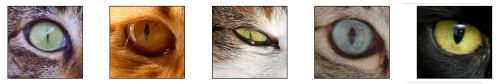
\includegraphics[width=\textwidth]{eyes}} 

\smallskip
  
\begin{center}
• • • • •
\end{center}
  
    
Program o wiele łatwiej jest napisać, gdy ma się przynajmniej mgliste pojęcie, do czego ma służyć. Dlatego poniżej przedstawiam plan aplikacji:

\begin{enumerate}
      \item Program rozpocznie działanie ze zbiorem kocich imion zawierającym tylko pozycję Spot.
      \item Program przejrzy wszystkie e-maile w chronologicznej kolejności.
      \item Program wyszuka akapity zaczynające się od słowa „urodzeni” lub „odeszli”.
      \item Program doda imiona z akapitów zaczynających się od słowa „urodzeni” do naszego zbioru.
      \item Program usunie imiona z akapitów zaczynających się od słowa „odeszli” z naszego zbioru.
\end{enumerate}
    
Pobieranie imion z akapitów będzie odbywać się następująco:

\begin{enumerate}
      \item Znalezienie w akapicie dwukropka.
      \item Pobranie tego, co znajduje się za dwukropkiem.
      \item Podzielenie pobranego tekstu na poszczególne imiona wg przecinków.
\end{enumerate}
    
Może się wydawać trochę ryzykowne zawierzenie, że ciotka Emilia zawsze stosuje dokładnie ten sam format i nigdy nie zapomina ani nie robi błędów w imionach, ale taka już właśnie ta ciotka jest.

  
  
\begin{center}
• • • • •
\end{center}
  
    
Najpierw opowiem Ci o własnościach\index{własności}. Z wieloma wartościami w języku JavaScript powiązane są inne wartości. Te powiązania nazywają się własnościami. Każdy łańcuch ma własność o nazwie \texttt{length}\index{length}, która odnosi się do liczby oznaczającej, z ilu znaków ten łańcuch się składa.

    
\index{[]}Dostęp do własności można uzyskać na dwa sposoby:

    
\begin{verbatim} 
var text = "fioletowa mgiełka";
show(text["length"]);
// → 17
show(text.length);
// → 17
\end{verbatim}
    
Drugi z przedstawionych rodzajów zapisu jest skrótem pierwszego i można go stosować tylko wtedy, gdy nazwa własności mogłaby być poprawną nazwą zmiennej ― nie zawiera spacji ani znaków specjalnych oraz nie zaczyna się od cyfry.

    
Wartości \texttt{null} i \texttt{undefined} nie mają żadnych własności. Próba odczytania własności jednej z nich zakończy się spowodowaniem błędu. Jeśli chcesz zobaczyć, jakie powiadomienia o błędach mogą wyświetlać przeglądarki (w~niektórych te komunikaty wyglądają bardzo tajemniczo), gdy napotkają taki kod, wykonaj poniższy program.

    
\begin{verbatim} 
var nothing = null;
show(nothing.length);
// → Exception: TypeError: nothing is null
\end{verbatim}
 
  
\begin{center}
• • • • •
\end{center}
  
    
Własności wartości łańcuchowej nie można zmieniać. Własność \texttt{length} to tylko jedna z wielu własności i nie można żadnych usuwać ani dodawać.

    
Z wartościami typu obiektowego\index{obiekt} jest jednak inaczej. Ich najważniejszą rolą jest właśnie przechowywać inne wartości. Można powiedzieć, że wartości te mają zestaw przyssawek w postaci własności. Można ja modyfikować, usuwać, a nawet dodawać nowe.

    
\index{\{\}}Obiekt można zapisać następująco:

    
\begin{verbatim} 
var cat = {colour: "grey", name: "Spot", size: 46};
cat.size = 47;
show(cat.size);
// → 47
delete cat.size;
show(cat.size);
// → undefined
show(cat);
// → {colour: "grey", name: "Spot"}
\end{verbatim}
    
Podobnie jak zmienne, każda własność związana z obiektem ma tekstową etykietę. Pierwsza z powyższych instrukcji tworzy obiekt, w którym znajduje się własność \texttt{"colour"} odnosząca się do łańcucha \texttt{"grey"}, własność \texttt{"name"} odnosząca się do łańcucha \texttt{"Spot"} oraz własność \texttt{"size"} odnosząca się do liczby \texttt{46}. Druga instrukcja przypisuje własności \texttt{size} nową wartość, co robi się w taki sam sposób, jak modyfikacja wartości zmiennej.

    
Słowo kluczowe \texttt{delete}\index{delete} usuwa własności. Próba odczytu nieistniejącej własności powoduje zwrócenie wartości \texttt{undefined}.

    
Jeżeli operator \texttt{=}\index{=} zostanie użyty do ustawienia własności, która jeszcze nie istnieje, to taka własność zostanie utworzona i dodana do obiektu.

    
\begin{verbatim} 
var empty = {};
empty.notReally = 1000;
show(empty.notReally);
// → 1000
\end{verbatim}
    
Własności, których nazwy nie mogłyby zostać użyte jako nazwy zmiennych muszą przy tworzeniu obiektu znajdować się w cudzysłowach, a gdy się ich potem używa, trzeba używać kwadratowych nawiasów:

    
\begin{verbatim} 
var thing = {"gabba gabba": "hey", "5": 10};
show(thing["5"]);
// → 10
thing["5"] = 20;
show(thing[2 + 3]);
// → 20
delete thing["gabba gabba"];
\end{verbatim}
    
Jak widać, w nawiasach kwadratowych może znajdować się dowolne wyrażenie. Jest ono konwertowane na łańcuch, aby można było określić nazwę własności, do której się odnosi. Jako nazw własności można używać nawet zmiennych:

    
\begin{verbatim} 
var propertyName = "length";
var text = "mainline";
show(text[propertyName]);
// → 8
\end{verbatim}
    
Do sprawdzenia czy obiekt ma określoną własność służy operator \texttt{in}\index{in}. Zwraca on wartość logiczną.

    
\begin{verbatim} 
var chineseBox = {};
chineseBox.content = chineseBox;
show("content" in chineseBox);
// → true
show("content" in chineseBox.content);
// → true
\end{verbatim}
  
  
\begin{center}
• • • • •
\end{center}
  
    
Gdy w konsoli wyświetlone są wartości obiektów, można je kliknąć, aby zbadać ich własności. Powoduje to zamianę okna wyjściowego na okno inspekcji. Kliknięcie znajdującego się w prawym górnym rogu tego okna znaku „x” powoduje powrót do okna wyjściowego, natomiast strzałka służy do przejścia do własności poprzednio badanego obiektu.

    
\begin{verbatim} 
show(chineseBox);
// → {content: {…}}
\end{verbatim}
  
  
\begin{center}
• • • • •
\end{center}
  
    
\section*{Ćwiczenie 4.1}
\label{sec:4.1}
    
      
W rozwiązaniu problemu z kotami wymienione zostało słowo „zbiór”\index{zbiór}. Zbiór to zestaw wartości, w którym żadna wartość nie może się powtórzyć. Jeśli imiona są łańcuchami, czy wiesz, jak użyć obiektu do reprezentowania zbioru imion?

      
Pokaż jak dodać i usunąć imię z tego zbioru oraz jak sprawdzić, czy dane imię w nim występuje.

    
[\hyperref[sol:4.1]{pokaż rozwiązanie}]
    
    
  
  
\begin{center}
• • • • •
\end{center}
  
    
\index{zmienialność}Jak widać, wartości obiektów mogą się zmieniać. Typy wartości opisane w~\hyperref[chap:2]{rozdziale 2} są niezmienne, tzn. nie można zmienić istniejących wartości tych typów. Można je łączyć i tworzyć z nich nowe wartości, ale jeśli weźmiemy dowolną wartość łańcuchową, to znajdującego się w niej tekstu nie możemy zmienić. Natomiast w obiektach treść wartości można zmieniać poprzez zmianę ich własności.

    
Jeśli mamy dwie liczby \texttt{120} i \texttt{120}, to praktycznie zawsze możemy je uważać za dokładnie tę samą liczbę. W przypadku obiektów posiadanie dwóch referencji do tego samego obiektu i posiadanie dwóch różnych obiektów zawierających takie same własności to nie to samo. Rozważmy poniższy przykład:

    
\begin{verbatim} 
var object1 = {value: 10};
var object2 = object1;
var object3 = {value: 10};

show(object1 == object2);
// → true
show(object1 == object3);
// → false

object1.value = 15;
show(object2.value);
// → 15
show(object3.value);
// → 10
 \end{verbatim}
    
\texttt{object1} i \texttt{object2} to dwie zmienne mające \emph{tę samą} wartość. Tak naprawdę jest tylko jeden obiekt i dlatego zmiana wartości obiektu \texttt{object1} powoduje również zmianę wartości obiektu \texttt{object2}. Zmienna \texttt{object3} wskazuje inne obiekt, który początkowo ma takie same własności, jak \texttt{object1}, ale jest osobnym obiektem.

    
Operator \texttt{==}\index{==} języka JavaScript przy porównywaniu obiektów zwraca wartość \texttt{true} tylko wtedy, gdy oba argumenty są dokładnie tą samą wartością. Wynik porównywania różnych obiektów o identycznej zawartości będzie negatywny (\texttt{false}). W niektórych przypadkach jest to przydatne, a w innych niepraktyczne.

  
  
\begin{center}
• • • • •
\end{center}
  
    
Wartości obiektowe mogą być używane do wielu różnych celów. Tworzenie zbioru to tylko jeden z nich. W tym rozdziale poznasz jeszcze kilka zastosowań tych struktur, a kolejne ważne sposoby ich użycia zostały opisane w \hyperref[chap:8]{rozdziale 8}.

    
W planie rozwiązania problemu z kotami ― w istocie lepiej mówić na to \emph{algorytm}, dzięki czemu inni będą myśleli, że wiemy o czym mówimy ― w~algorytmie, jest mowa o przejrzeniu wszystkich e-maili znajdujących się w~archiwum. Jak wygląda te archiwum? I gdzie się znajduje?

    
Drugim z tych pytań na razie się nie przejmuj. W \hyperref[chap:14]{rozdziale 14} poznasz kilka sposobów importowania danych do programów, a na razie przyjmiemy, że e-maile w jakiś magiczny sposób stały się dostępne. W komputerach czarowanie jest naprawdę łatwe.

  
  
\begin{center}
• • • • •
\end{center}
  
    
Sposób przechowywania archiwum jest jednak ciekawą kwestią. W archiwum znajduje się pewna liczba e-maili. Wiadomość e-mail, co oczywiste, może być łańcuchem. W związku z tym całe archiwum można by było umieścić w jednym wielkim łańcuchu, ale to by było niepraktyczne. Potrzebujemy kolekcji osobnych łańcuchów.

    
Do przechowywania kolekcji łańcuchów dobrze nadają się obiekty. Można np. utworzyć obiekt w ten sposób:

    
\begin{verbatim} 
var mailArchive = {"Pierwszy e-mail": "Drogi siostrzeńcu, ...",
                   "Drugi e-mail": "..."
                   /* itd. ... */};
 \end{verbatim}
    
Ale w ten sposób trudno by było przejrzeć e-maile od początku do końca, bo skąd program ma wiedzieć, jakie są nazwy własności? Z tym problemem można sobie poradzić stosując przewidywalne nazwy własności:

    
\begin{verbatim} 
var mailArchive = {0: "Drogi siostrzeńcu, ... (mail 1)",
                   1: "(mail 2)",
                   2: "(mail 3)"};

for (var current = 0; current in mailArchive; current++)
  print("Przetwarzanie e-maila nr ", current, ": ", mailArchive[current]);
// → Przetwarzanie e-maila nr 0: Drogi siostrzeńcu, ... (mail 1)
// → Przetwarzanie e-maila nr 1: (mail 2)
// → Przetwarzanie e-maila nr 2: (mail 3)
\end{verbatim}
    
Mamy szczęście, że istnieje specjalny rodzaj obiektów przeznaczony właśnie do takich zastosowań. Jest to tablica\index{tablica}, która dodatkowo zawiera pewne udogodnienia, jak np. własność \texttt{length}\index{length} pozwalająca sprawdzić, ile wartości się w niej znajduje oraz obsługuje różne przydatne rodzaje operacji.

    
\index{[]}Nowe tablice tworzy się przy użyciu kwadratowych nawiasów (\texttt{[} i \texttt{]}):

    
\begin{verbatim} 
var mailArchive = ["e-mail 1", "e-mail 2", "e-mail 3"];

for (var current = 0; current < mailArchive.length; current++)
  print("Przetwarzanie e-maila nr ", current, ": ", mailArchive[current]);
// → Przetwarzanie e-maila nr 0: e-mail 1
// → Przetwarzanie e-maila nr 1: e-mail 2
// → Przetwarzanie e-maila nr 2: e-mail 3
\end{verbatim}
    
W tym przykładzie numery elementów nie są definiowane bezpośrednio. Pierwszemu automatycznie przypisywany jest numer 0, drugiemu — 1 itd.

    
Dlaczego numerowanie zaczyna się od 0? Ludzie zwykle zaczynają liczyć od 1. Jednak w przypadku kolekcji elementów bardziej praktyczne jest rozpoczynanie liczenia od 0. Po prostu zaakceptuj to, a z czasem się przyzwyczaisz.

    
Skoro numeracja rozpoczyna się od 0, to znaczy, że w kolekcji \texttt{X} elementów ostatni element ma numer \texttt{X - 1}. Dlatego właśnie w pętli \texttt{for} w powyższym przykładzie znajduje się warunek \texttt{current < mailArchive.length}. Na pozycji \texttt{mailArchive.length} nie ma żadnego elementu, a więc gdy zmienna \texttt{current} uzyska tę wartość, kończymy iterowanie.

  
  
\begin{center}
• • • • •
\end{center}
  
    
\section*{Ćwiczenie 4.2}
\label{sec:4.2}
    
      
Napisz funkcję o nazwie \texttt{range} przyjmującą jako argument liczbę całkowitą i~zwracającą tablicę wszystkich liczb od 0 do tej liczby włącznie.

      
Pustą tablicę można utworzyć pisząc \texttt{[]}. Pamiętaj też, że własności do obiektów, a więc też i tablic, można dodawać przypisując im wartości za pomocą operatora \texttt{=}. Własność \texttt{length} jest aktualizowana automatycznie, gdy są dodawane kolejne elementy.

    
[\hyperref[sol:4.2]{pokaż rozwiązanie}]
    
    
  
  
\begin{center}
• • • • •
\end{center}
  
    
Zarówno obiekty łańcuchowe jak i tablicowe oprócz własności \texttt{length} zawierają jeszcze kilka innych własności odnoszących się do wartości funkcyjnych.

    
\begin{verbatim} 
var doh = "Doh";
print(typeof doh.toUpperCase);
// → function
print(doh.toUpperCase());
// → DOH
\end{verbatim}
    
Każdy łańcuch ma własność \texttt{toUpperCase}\index{toUpperCase}. Własność ta zwraca kopię łańcucha, w której wszystkie litery są wielkie. Istnieje też własność \texttt{toLowerCase}\index{toLowerCase}. Zgadnij do czego służy.

    
Zwróć też uwagę, że mimo iż w wywołaniu \texttt{toUpperCase} nie przekazano żadnych argumentów, funkcja ta w jakiś sposób uzyskała dostęp do łańcucha \texttt{"Doh"}, wartości, której jest własnością. Szczegółowo działanie tego mechanizmu jest opisane w \hyperref[chap:8]{rozdziale 8}.

    
Własności zawierające funkcje nazywają się metodami\index{metoda}, a więc \texttt{toUpperCase} jest metodą obiektu łańcuchowego.

    
\begin{verbatim} 
var mack = [];
mack.push("Mack");
mack.push("the");
mack.push("Knife");
show(mack.join(" "));
// → "Mack the Knife"
show(mack.pop());
// → "Knife"
show(mack);
// → ["Mack", "the"]
\end{verbatim}
    
Metoda \texttt{push}\index{push}, która jest związana z tablicami, służy do dodawania wartości do tych struktur. Można by jej było użyć w ostatnim ćwiczeniu zamiast  instrukcji \texttt{result[i] = i}. Istnieje też metoda \texttt{pop}\index{pop}, która jest przeciwieństwem metody \texttt{push}: usuwa i zwraca ostatnią wartość tablicy. Metoda \texttt{join}\index{join} tworzy pojedynczy długi łańcuch z tablicy łańcuchów. Parametr jej wywołania jest wstawiany między wartościami tablicy.

  
  
\begin{center}
• • • • •
\end{center}
  
    
Wracając do kotów, wiemy już, że do przechowywania archiwum e-maili doskonale nada się tablica. Na tej stronie tablicę tę można magicznie pobrać za pomocą funkcji \texttt{retrieveMails}. Przejrzenie e-maili i ich przetworzenie nie będzie już teraz wielkim wyzwaniem:

    
\begin{verbatim} 
var mailArchive = retrieveMails();

for (var i = 0; i < mailArchive.length; i++) {
  var email = mailArchive[i];
  print("Przetwarzanie e-maila nr ", i);
  // Jakieś działania...
}
// → Przetwarzanie e-maila nr 0
// → Przetwarzanie e-maila nr 1
// → ... itd.
\end{verbatim}
    
Wybraliśmy też sposób reprezentacji zbioru kotów, które wciąż żyją. Zatem następnym problemem jest znalezienie w wiadomości e-mail akapitów zaczynających się od słów \texttt{"urodzeni"} lub \texttt{"odeszli"}.

  
  
\begin{center}
• • • • •
\end{center}
  
    
Od razu nasuwa się pytanie, czym jest akapit. W tym przypadku odpowiedź wartość łańcuchowa nie będzie pomocna, ponieważ w języku JavaScript tekstem jest po prostu „szereg znaków”, a więc musimy sami zdefiniować akapity bazując na tym, co mamy.

    
Wcześniej pokazałem Ci, że istnieje coś takiego, jak znak nowego wiersza. Zazwyczaj znak ten jest używany do oddzielania akapitów. W związku z~tym za akapit będziemy uznawać część wiadomości e-mail, której początek wyznacza znak nowego wiersza lub początek treści, a koniec określa kolejny znak nowego wiersza lub koniec treści.

    
Nie musimy nawet samodzielnie pisać algorytmu do dzielenia łańcucha na akapity. Łańcuchy mają gotową metodę o nazwie \texttt{split}\index{split}, która jest prawie dokładnym przeciwieństwem metody \texttt{join} w tablicach. Metoda ta tnie łańcuch na fragmenty, które zapisuje w elementach tablicy, a jako znaku podziału używa łańcucha przekazanego jej jako argument.

    
\begin{verbatim} 
var words = "Cities of the Interior";
show(words.split(" "));
// → ["Cities", "of", "the", "Interior"]
\end{verbatim}
    
W związku z tym do podzielenia wiadomości e-mail na akapity możemy zastosować cięcie wg znaków nowego wiersza (\texttt{"\textbackslash n"}).

  
  
\begin{center}
• • • • •
\end{center}
  
    
\section*{Ćwiczenie 4.3}
\label{sec:4.3}
    
      
Metody \texttt{split} i \texttt{join} nie są swoimi dokładnymi przeciwieństwami. Instrukcja \texttt{string.split(x).join(x)} zawsze zwróci oryginalną wartość, ale \texttt{array.join(x)\\.split(x)} nie. Potrafisz podać przykład tablicy, dla której instrukcja \texttt{.join(" ").split(" ")} zwróci inną wartość?

    
[\hyperref[sol:4.3]{pokaż rozwiązanie}]
    
    
  
  
\begin{center}
• • • • •
\end{center}
  
    
Akapity nie rozpoczynające się od słów „urodzeni” i „odeszli” mogą zostać zignorowane. Jak sprawdzić, czy łańcuch zaczyna się od określonego słowa? Za pomocą metody \texttt{charAt}\index{charAt} można pobrać wybraną literę z łańcucha. Instrukcja \texttt{x.charAt(0)} zwraca pierwszą literę, \texttt{1} — drugą itd. Jednym ze sposobów na sprawdzenie, czy łańcuch zaczyna się od słowa „urodzeni” jest napisanie takiego kodu:

    
\begin{verbatim} 
var paragraph = "urodzeni 15-11-2003 (matka Spot): White Fang";
show(paragraph.charAt(0) == "u" && paragraph.charAt(1) == "r" &&
     paragraph.charAt(2) == "o" && paragraph.charAt(3) == "d") &&
     paragraph.charAt(4) == "z" && paragraph.charAt(5) == "e" &&
     paragraph.charAt(6) == "n" && paragraph.charAt(7) == "i";
// → true
\end{verbatim}
    
Ale to nie jest eleganckie rozwiązanie ― wyobraź sobie sprawdzanie słów składających się z jeszcze większej liczby liter. Możesz się tu jednak czegoś nauczyć: jeśli wiersz kodu staje się zbyt długi, można go podzielić na kilka wierszy. Aby tekst programu był przejrzysty, można wyrównać początek nowego wiersza z pierwszym podobnym elementem poprzedniego wiersza.

    
Łańcuchy mają też metodę o nazwie \texttt{slice}\index{slice}. Metoda ta kopiuje fragment łańcucha zaczynając od miejsca określonego liczbowo w pierwszym argumencie i kończąc przed znakiem znajdującym się na pozycji wyznaczonej przez drugi argument (tez znak nie jest wliczany). Przy jej użyciu nasz test możemy zapisać krócej.

    
\begin{verbatim} 
show(paragraph.slice(0, 8) == "urodzeni");
// → true
\end{verbatim}
  
  
\begin{center}
• • • • •
\end{center}
  
    
\section*{Ćwiczenie 4.4}
\label{sec:4.4}
    
      
Napisz funkcję o nazwie \texttt{startsWith}, która pobiera dwa argumenty łańcuchowe. Niech zwraca wartość \texttt{true}, gdy pierwszy argument zaczyna się od znaków znajdujących się w drugim argumencie i \texttt{false} w przeciwnym przypadku.

    
[\hyperref[sol:4.4]{pokaż rozwiązanie}]
    
    
  
  
\begin{center}
• • • • •
\end{center}
  
    
Co się dzieje, gdy metody \texttt{charAt} i \texttt{slice} zostaną użyte do pobrania nieistniejącego fragmentu łańcucha? Czy funkcja \texttt{startsWith} będzie działać nawet wtedy, gdy szukany łańcuch (pattern) będzie dłuższy od łańcucha, w~którym ma być szukany?

    
\begin{verbatim} 
show("Pip".charAt(250));
// → ""
show("Nop".slice(1, 10));
// → "op"
 \end{verbatim}
    
Metoda \texttt{charAt} dla nieistniejącego znaku zwraca \texttt{""}, a \texttt{slice} po prostu ignoruje tę część, która nie istnieje.

    
A zatem odpowiedź na postawione pytanie brzmi „tak, funkcja \texttt{startsWith} będzie działać”. W wywołaniu \texttt{startsWith("Idioci", "najbardziej szanowani koledzy")}, wywołanie metody \texttt{slice} zawsze zwróci łańcuch krótszy od \texttt{pattern}, ponieważ argument \texttt{string} nie zawiera wystarczająco dużo znaków. Z tego powodu wynikiem porównywania przy użyciu operatora \texttt{==} będzie \texttt{false}, czyli to, co powinno.

    
Zawsze warto chwilę zastanowić się nad nienormalnymi (ale poprawnymi) danymi wejściowymi do programu. Są to tzw. przypadki brzegowe\index{przypadki brzegowe} i wiele programów, które działają doskonale na wszystkich „normalnych” danych wejściowych fiksuje właśnie na tych przypadkach.

  
  
\begin{center}
• • • • •
\end{center}
  
    
Z problemu z kotami nierozwiązana pozostała już tylko kwestia pobierania imion z akapitów. Opis algorytmu wyglądał tak:

    \begin{enumerate}
      \item Znalezienie w akapicie dwukropka.
      \item Pobranie tego, co znajduje się za dwukropkiem.
      \item Podzielenie pobranego tekstu na poszczególne imiona wg przecinków.
    \end{enumerate}
    
Dotyczy to zarówno akapitów zaczynających się od słowa \texttt{"odeszli"} jak i od słowa \texttt{"urodzeni"}. Dobrym pomysłem jest zapisanie tego algorytmu jako funkcji, aby można go było używać w kodzie obsługującym oba rodzaje akapitów.

  
  
\begin{center}
• • • • •
\end{center}
  
    
\section*{Ćwiczenie 4.5}
\label{sec:4.5}
    
      
Potrafisz napisać funkcję o nazwie \texttt{catNames}, która jako argument pobiera akapit i zwraca tablicę imion?

      
Łańcuchy mają metodę \texttt{indexOf}\index{indexOf}, za pomocą której można znaleźć pozycję pierwszego wystąpienia znaku lub podłańcucha w łańcuchu. Ponadto metoda \texttt{slice}, gdy przekaże się jej tylko jeden argument zwraca część łańcucha od określonej w tym argumencie pozycji do końca.

      
Pomóc może Ci użycie konsoli do zbadania sposobu, w jaki działają funkcje. Wpisz np. \texttt{"foo: bar".indexOf(":")} i zobacz, co się stanie.

    
[\hyperref[sol:4.5]{pokaż rozwiązanie}]
    
    
  
  
\begin{center}
• • • • •
\end{center}
  
    
Pozostało więc tylko poskładać wszystkie części w jedną całość. Oto jeden ze sposobów:

    
\begin{verbatim} 
var mailArchive = retrieveMails();
var livingCats = {"Spot": true};

for (var mail = 0; mail < mailArchive.length; mail++) {
  var paragraphs = mailArchive[mail].split("\n");
  for (var paragraph = 0;
       paragraph < paragraphs.length;
       paragraph++) {
    if (startsWith(paragraphs[paragraph], "urodzeni")) {
      var names = catNames(paragraphs[paragraph]);
      for (var name = 0; name < names.length; name++)
        livingCats[names[name]] = true;
    }
    else if (startsWith(paragraphs[paragraph], "odeszli")) {
      var names = catNames(paragraphs[paragraph]);
      for (var name = 0; name < names.length; name++)
        delete livingCats[names[name]];
    }
  }
}

show(livingCats);
// → {Clementine: true, Black Leclère: true, …}
\end{verbatim}
    
To dość długi i skomplikowany kod. Zaraz spróbujemy sprawić, aby wyglądał trochę klarowniej. Ale najpierw spójrz na wyniki. Wiemy, jak sprawdzić czy określony kot żyje:

    
\begin{verbatim} 
if ("Spot" in livingCats)
  print("Spot żyje!");
else
  print("Dobra stara Spot, niech spoczywa w pokoju.");
// → Dobra stara Spot, niech spoczywa w pokoju.
\end{verbatim}
    
A jak wyświetlić listę wszystkich żyjących kotów? Słowo kluczowe \texttt{in}\index{in}, gdy zostanie użyte w połączeniu z \texttt{for} nieco zmienia swoje znaczenie:

    
\begin{verbatim} 
for (var cat in livingCats)
  print(cat);
// → Clementine
// → Black Leclère
// → ... itd.
\end{verbatim}
    
Powyższa pętla przegląda nazwy własności w obiekcie, dzięki czemu możemy zrobić listę wszystkich imion znajdujących się w naszym zbiorze.

  
  
\begin{center}
• • • • •
\end{center}
  
    
Niektóre fragmenty kodu wyglądają, jak gęsta dżungla. Dotyczy to także naszego rozwiązania kociego problemu. Jednym ze sposobów na poprawienie czytelności kodu jest dodanie do niego trochę pustych wierszy. Teraz kod wygląda lepiej, ale to nie rozwiązuje całkowicie problemu.

    
Żeby osiągnąć sukces, powinniśmy ten kod podzielić. Napisaliśmy już dwie funkcje pomocnicze, \texttt{startsWith} i \texttt{catNames}, z których każda rozwiązuje niewielki i dający się ogarnąć myślą fragment problemu. Możemy dalej rozwijać to podejście.

    
\begin{verbatim} 
function addToSet(set, values) {
  for (var i = 0; i < values.length; i++)
    set[values[i]] = true;
}

function removeFromSet(set, values) {
  for (var i = 0; i < values.length; i++)
    delete set[values[i]];
}
 \end{verbatim}
    
Te dwie funkcje dodają imiona do zbioru i je z niego usuwają. Dzięki nim możemy pozbyć się dwóch najgłębiej położonych pętli z rozwiązania:

    
\begin{verbatim} 
var livingCats = {Spot: true};

for (var mail = 0; mail < mailArchive.length; mail++) {
  var paragraphs = mailArchive[mail].split("\n");
  for (var paragraph = 0;
       paragraph < paragraphs.length;
       paragraph++) {
    if (startsWith(paragraphs[paragraph], "urodzeni"))
      addToSet(livingCats, catNames(paragraphs[paragraph]));
    else if (startsWith(paragraphs[paragraph], "odeszli"))
      removeFromSet(livingCats, catNames(paragraphs[paragraph]));
  }
}
 \end{verbatim}
    
Całkiem nieźle, jeśli mogę sam siebie pochwalić.

    
Dlaczego funkcje \texttt{addToSet} i \texttt{removeFromSet} pobierają zbiór jako argument? Równie dobrze mogłyby bezpośrednio używać zmiennej \texttt{livingCats}. Ale dzięki zastosowanemu podejściu nie są ściśle związane z tym jednym problemem. Gdyby funkcja \texttt{addToSet} bezpośrednio operowała na zmiennej \texttt{livingCats}, musiałaby się nazywać \texttt{addCatsToCatSet} lub jakoś podobnie. Dzięki takiej budowie, jak ma teraz jest bardziej ogólna.

    
Funkcje warto pisać w taki sposób nawet wtedy, gdy nie planuje się ich kiedykolwiek używać do innych celów, co jest całkiem możliwe. Dzięki temu, że są „samowystarczalne”, można je czytać i zrozumieć bez potrzeby dowiadywania się, czym jest jakaś zewnętrzna zmienna o nazwie \texttt{livingCats}.

    
Te funkcje nie są czyste, ponieważ zmieniają obiekt, który zostaje im przekazany jako argument \texttt{set}. To sprawia, że są trochę trudniejsze od prawdziwych czystych funkcji, ale i tak o wiele mniej skomplikowane niż funkcje, które jak szaleniec zmieniają każdą wartość i zmienną, jaką mają ochotę zmienić.

  
  
\begin{center}
• • • • •
\end{center}
  
    
Kontynuujemy omawianie algorytmu:

    
\begin{verbatim} 
function findLivingCats() {
  var mailArchive = retrieveMails();
  var livingCats = {"Spot": true};

  function handleParagraph(paragraph) {
    if (startsWith(paragraph, "urodzeni"))
      addToSet(livingCats, catNames(paragraph));
    else if (startsWith(paragraph, "odeszli"))
      removeFromSet(livingCats, catNames(paragraph));
  }

  for (var mail = 0; mail < mailArchive.length; mail++) {
    var paragraphs = mailArchive[mail].split("\n");
    for (var i = 0; i < paragraphs.length; i++)
      handleParagraph(paragraphs[i]);
  }
  return livingCats;
}

var howMany = 0;
for (var cat in findLivingCats())
  howMany++;
print("Jest ", howMany, " kotów.");
// → Jest 22 kotów.
\end{verbatim}
    
Teraz cały algorytm znajduje się w funkcji. Dzięki temu po zakończeniu działania nie pozostawi bałaganu. Zmienna \texttt{livingCats} jest teraz lokalna w~funkcji, a więc istnieje tylko w czasie, gdy ta funkcja jest wykonywana. Kod potrzebujący tego zbioru może wywołać funkcję \texttt{findLivingCats} i użyć jej wartości zwrotnej.

    
Ponadto wydawało mi się, że utworzenie osobnej funkcji \texttt{handleParagraph} również sprawi, że kod będzie bardziej przejrzysty. Jest ona jednak ściśle związana z kocim algorytmem i w innych sytuacjach byłaby nieprzydatna. Ponadto potrzebny jest jej dostęp do zmiennej \texttt{livingCats}. To wszystko sprawia, że funkcja ta doskonale nadaje się do zdefiniowania w innej funkcji. Umieszczając ją w funkcji \texttt{findLivingCats} podkreślamy, że jest przydatna tylko w niej i udostępniamy jej zmienne tej funkcji nadrzędnej.

    
To rozwiązanie jest tak naprawdę \emph{większe} od poprzedniego. Ale jest za to klarowniejsze i chyba się zgodzisz, że bardziej czytelne.

  
  
\begin{center}
• • • • •
\end{center}
  
    
Program nadal ignoruje wiele informacji znajdujących się w e-mailach. Można w nich znaleźć daty urodzin, daty śmierci oraz imiona matek.

    
Zaczniemy od dat. Jaki jest najlepszy sposób ich przechowywania? Moglibyśmy utworzyć obiekt z własnościami \texttt{year}, \texttt{month} i \texttt{day} i w nich zapisać odpowiednie liczby.

    
\begin{verbatim} 
var when = {year: 1980, month: 2, day: 1};
\end{verbatim}
    
Ale w języku JavaScript dostępny jest gotowy obiekt do przechowywania tego typu danych. Można go utworzyć przy użyciu słowa kluczowego \texttt{new}\index{new}

    
\begin{verbatim} 
var when = new Date(1980, 1, 1);
show(when);
// → Fri Feb 01 1980 00:00:00 GMT+0100
\end{verbatim}
    
Do tworzenia wartości obiektowych można używać słowa kluczowego \texttt{new}, podobnie jak nawiasów klamrowych z dwukropkami. Jednak zamiast podawać nazwy i wartości wszystkich własności, w tym przypadku obiekt tworzy się przy użyciu funkcji. Dzięki temu możliwe jest opracowanie standardowych procedur tworzenia obiektów. Funkcje tego typu nazywają się konstruktorami\index{konstruktor}, a techniki ich tworzenia poznasz w \hyperref[chap:8]{rozdziale 8}.

    
Konstruktora \texttt{Date}\index{Date} można używać na różne sposoby.

    
\begin{verbatim} 
show(new Date());
show(new Date(1980, 1, 1));
// → Fri Feb 01 1980 00:00:00 GMT+0100
show(new Date(2007, 2, 30, 8, 20, 30));
// → Fri Mar 30 2007 08:20:30 GMT+0200
\end{verbatim}
    
Jak widać, w obiektach tych można przechowywać zarówno godziny jak i~daty. Jeśli nie przekaże się żadnych argumentów, zostanie utworzony obiekt zawierający bieżącą datę i godzinę. Jeśli się je zdefiniuje, to można za ich pomocą utworzyć obiekt zawierający wybraną datę i godzinę. Argumenty te kolejno oznaczają rok, miesiąc, dzień, godzinę, minutę, sekundę oraz milisekundę. Cztery ostatnie argumenty są opcjonalne i jeśli nie zostaną zdefiniowane, nadawana jest im wartość 0.

    
Miesiące w tych obiektach są numerowane od 0 do 11, co może powodować pomyłki. Co ciekawe, numeracja dni zaczyna się od 1.

  
  
\begin{center}
• • • • •
\end{center}
  
    
Zawartość obiektu \texttt{Date} można zbadać przy użyciu metod \texttt{get...}.

    
\begin{verbatim} 
var today = new Date();
print("Rok: ", today.getFullYear(), ", miesiąc: ",
      today.getMonth(), ", dzień: ", today.getDate());
print("Godzina: ", today.getHours(), ", minuta: ",
      today.getMinutes(), ", sekunda: ", today.getSeconds());
print("Dzień tygodnia: ", today.getDay());
 \end{verbatim}
    
Wszystkie te metody oprócz \texttt{getDay} mają również odpowiednik z przedrostkiem \texttt{set}, który służy do zmieniania wartości obiektu.

    
Wewnątrz obiektu data jest reprezentowana w postaci liczby milisekund, jaka upłynęła od 1 stycznia 1970 r. Domyślasz się pewnie, że to całkiem spora liczba.

    
\begin{verbatim} 
var today = new Date();
show(today.getTime());
\end{verbatim}
    
Jedną z najczęściej wykonywanych operacji na datach jest porównywanie.

    
\begin{verbatim} 
var wallFall = new Date(1989, 10, 9);
var gulfWarOne = new Date(1990, 6, 2);
show(wallFall < gulfWarOne);
// → true
show(wallFall == wallFall);
// → true
// ale
show(wallFall == new Date(1989, 10, 9));
// → false
\end{verbatim}
    
Wyniki porównywania dat za pomocą operatorów \texttt{<}, \texttt{>}, \texttt{<=} oraz \texttt{>=} są prawidłowe. Gdy obiekt daty porówna się z nim samym za pomocą operatora \texttt{==}, zwrócona zostanie wartość \texttt{true}, co również jest dobre. Jeśli jednak za pomocą operatora \texttt{==}\index{==} porówna się dwa różne obiekty daty zawierające tę samą datę, zostanie zwrócony wynik \texttt{false}. Dlaczego?

    
Już wcześniej napisałem, że operator \texttt{==} zawsze zwraca wartość \texttt{false}, gdy porównywane są dwa różne obiekty, nawet jeżeli zawierają one identyczne własności. Jest to trochę niezgrabne i mylące rozwiązanie, ponieważ logicznie rzecz biorąc można się spodziewać, że operatory \texttt{>=} i \texttt{==} powinny działać podobnie. Aby sprawdzić czy dwie daty są sobie równe, można napisać taki kod:

    
\begin{verbatim} 
var wallFall1 = new Date(1989, 10, 9),
    wallFall2 = new Date(1989, 10, 9);
show(wallFall1.getTime() == wallFall2.getTime());
// → true
\end{verbatim}
  
  
\begin{center}
• • • • •
\end{center}
  
    
Oprócz daty i godziny obiekty \texttt{Date} zawierają dodatkowo informację o~strefie czasowej\index{strefa czasowa}. Gdy w Amsterdamie jest trzynasta, to w niektórych porach roku w Londynie jest południe, a w Nowym Jorku siódma. Godziny można zatem porównywać tylko, gdy weźmie się pod uwagę strefę czasową. Za pomocą funkcji \texttt{getTimezoneOffset}\index{getTimezoneOffset} obiektu \texttt{Date} można sprawdzić, o ile minut godzina zawarta w tym obiekcie różni się od czasu GMT (Greenwich Mean Time).

    
\begin{verbatim} 
var now = new Date();
print(now.getTimezoneOffset());
// → -120
\end{verbatim}
  
  
\begin{center}
• • • • •
\end{center}
  
    
\section*{Ćwiczenie 4.6}
\label{sec:4.6}
    
      
\begin{verbatim} 
"odeszli 27.04.2006: Black Leclère"
 \end{verbatim}
      
Data zawsze znajduje się w tym samym miejscu akapitu. Jak fajnie. Napisz funkcję o nazwie \texttt{extractDate} pobierającą taki akapit jako argument i~wydobywającą z niego datę oraz zwracającą ją w obiekcie daty.

    
[\hyperref[sol:4.6]{pokaż rozwiązanie}]
    
    
  
  
\begin{center}
• • • • •
\end{center}
  
    
Od tej pory zapisywanie kotów będzie przebiegało inaczej. Zamiast tylko umieścić wartość \texttt{true} w zbiorze, teraz będziemy zapisywać obiekt z informacjami o kocie. Gdy kot zdechnie, nie będziemy go usuwać ze zbioru, tylko dodamy do obiektu własność \texttt{death}, w której zapiszemy datę śmierci zwierzęcia.

    
Z tego powodu funkcje \texttt{addToSet} i \texttt{removeFromSet} stały się bezużyteczne. Potrzebujemy czegoś podobnego, ale to coś musi dodatkowo zapisywać datę urodzenia i imię matki.

    
\begin{verbatim} 
function catRecord(name, birthdate, mother) {
  return {name: name, birth: birthdate, mother: mother};
}

function addCats(set, names, birthdate, mother) {
  for (var i = 0; i < names.length; i++)
    set[names[i]] = catRecord(names[i], birthdate, mother);
}
function deadCats(set, names, deathdate) {
  for (var i = 0; i < names.length; i++)
    set[names[i]].death = deathdate;
}
 \end{verbatim}
    
\texttt{catRecord} to osobna funkcja służąca do tworzenia tych magazynowych obiektów. Może być przydatna też w innych sytuacjach, jak np. utworzenie obiektu dla Spot. Słowo „Record” jest często używane w nazwach tego rodzaju obiektów, które służą do grupowania określonej ograniczonej liczby wartości.

  
  
\begin{center}
• • • • •
\end{center}
  
    
Spróbujmy więc pobrać imiona kocich matek z akapitów.

    
\begin{verbatim} 
"urodzeni 15/11/2003 (matka Spot): White Fang"
 \end{verbatim}
    
Oto jeden z możliwych sposobów…

    
\begin{verbatim} 
function extractMother(paragraph) {
  var start = paragraph.indexOf("(matka ") + "(matka ".length;
  var end = paragraph.indexOf(")");
  return paragraph.slice(start, end);
}

show(extractMother("urodzeni 15/11/2003 (matka Spot): White Fang"));
// → "Spot"
 \end{verbatim}
    
Zwróć uwagę, że pozycja startowa musi zostać dostosowana do długości słowa \texttt{"(matka "}, ponieważ \texttt{indexOf} zwraca pozycję początku wzorca, a nie jego końca.

  
  
\begin{center}
• • • • •
\end{center}
  
    
\section*{Ćwiczenie 4.7}
\label{sec:4.7}
    
      
Działanie wykonywane przez funkcję \texttt{extractMother} można wyrazić w bardziej ogólny sposób. Napisz funkcję o nazwie \texttt{between}, która pobiera trzy argumenty łańcuchowe. Funkcja ta niech zwraca część pierwszego argumentu, która występuje między wzorcami znajdującymi się w drugim i trzecim argumencie.

      
Na przykład wynikiem wywołania \texttt{between("urodzeni 15/11/2003 (matka Spot): White Fang", "(matka ", ")")} powinien być łańcuch \texttt{"Spot"}.

      
A wynikiem wywołania \texttt{between("bu ] boo [ bah ] gzz", "[ ", " ]")} powinien być łańcuch \texttt{"bah"}.

      
Drugi z wymienionych przypadków łatwiej będzie zaimplementować wiedząc, że funkcji \texttt{indexOf} można przekazać drugi, opcjonalny, argument określający, w którym miejscu ma się rozpocząć szukanie.

    
[\hyperref[sol:4.7]{pokaż rozwiązanie}]
    
    
  
  
\begin{center}
• • • • •
\end{center}
  
    
Dzięki funkcji \texttt{between} można uprościć funkcję extractMother:

    
\begin{verbatim} 
function extractMother(paragraph) {
  return between(paragraph, "(matka ", ")");
}
 \end{verbatim}
  
  
\begin{center}
• • • • •
\end{center}
  
    
Ulepszona wersja kociego algorytmu wygląda teraz tak:

    
\begin{verbatim} 
function findCats() {
  var mailArchive = retrieveMails();
  var cats = {"Spot": catRecord("Spot", new Date(1997, 2, 5),
              "nieznany")};

  function handleParagraph(paragraph) {
    if (startsWith(paragraph, "urodzeni"))
      addCats(cats, catNames(paragraph), extractDate(paragraph),
              extractMother(paragraph));
    else if (startsWith(paragraph, "odeszli"))
      deadCats(cats, catNames(paragraph), extractDate(paragraph));
  }

  for (var mail = 0; mail < mailArchive.length; mail++) {
    var paragraphs = mailArchive[mail].split("\n");
    for (var i = 0; i < paragraphs.length; i++)
      handleParagraph(paragraphs[i]);
  }
  return cats;
}

var catData = findCats();
 \end{verbatim}
    
Mając te dodatkowe dane możemy w końcu połapać się w kotach ciotki Emilii. Poniższa funkcja może być przydatna:

    
\begin{verbatim} 
function formatDate(date) {
  return date.getDate() + "/" + (date.getMonth() + 1) +
         "/" + date.getFullYear();
}

function catInfo(data, name) {
  if (!(name in data))
    return "Kot o imieniu " + name + " nie jest znany światu.";

  var cat = data[name];
  var message = name + ", urodzony " + formatDate(cat.birth) +
                " z matki  " + cat.mother;
  if ("death" in cat)
    message += ", zdechł dnia " + formatDate(cat.death);
  return message + ".";
}

print(catInfo(catData, "Fat Igor"));
// → Fat Igor, urodzony 30/11/1899 z matki  Miss Bushtail.
\end{verbatim}
    
Pierwsza instrukcja \texttt{return} w funkcji \texttt{catInfo} służy jako wyjście awaryjne. Jeśli o wybranym kocie nie ma żadnych danych, reszta funkcji jest bez znaczenia, w związku z czym od razu zwracamy wartość, aby wstrzymać dalsze niepotrzebne wykonywanie kodu.

    
Kiedyś niektórzy programiści funkcje zawierające kilka instrukcji \texttt{return} uważali za ciężki grzech. Chodziło im o to, że wówczas trudno jest określić, która część kodu zostanie wykonana, a która nie. W \hyperref[chap:5]{rozdziale 5} poznasz techniki, dzięki którym argumenty używane przez tych programistów stały się mniej lub bardziej nieaktualne, chociaż wciąż od czasu do czasu można spotkać osoby krytykujące taki sposób użycia instrukcji return.

  
  
\begin{center}
• • • • •
\end{center}
  
    
\section*{Ćwiczenie 4.8}
\label{sec:4.8}
    
      
Funkcja \texttt{formatDate} używana przez funkcję \texttt{catInfo} nie dodaje zera przed jednocyfrowymi numerami miesięcy i dni. Napisz jej nową wersję, która będzie to robić.

    
[\hyperref[sol:4.8]{pokaż rozwiązanie}]
    
  
\begin{center}
• • • • •
\end{center}
  
    
\section*{Ćwiczenie 4.9}
\label{sec:4.9}
    
      
Napisz funkcję o nazwie \texttt{oldestCat} przyjmującą jako argument obiekt zawierający dane kotów i zwracającą nazwę najstarszego żyjącego kota.

    
[\hyperref[sol:4.9]{pokaż rozwiązanie}] 
  
  
\begin{center}
• • • • •
\end{center}
  
    
Skoro wiesz już jak posługiwać się tablicami, pokażę Ci jeszcze coś innego. Gdy wywoływana jest jakakolwiek funkcja, w środowisku, w którym działa tworzona jest specjalna zmienna o nazwie \texttt{arguments}\index{arguments}. Zmienna ta odwołuje się do obiektu, który przypomina tablicę. Pierwszy argument jest własnością \texttt{0}, drugi argument jest własnością \texttt{1} itd. dla wszystkich argumentów, jakie zostały przekazane funkcji. Ponadto zmienna ta ma własność \texttt{length}\index{length}.

    
Obiekt ten nie jest jednak prawdziwą tablicą, nie ma takich metod, jak \texttt{push} i nie aktualizuje automatycznie swojej własności \texttt{length}, gdy zostanie do niego coś dodane. Nie udało mi się dowiedzieć, czemu nie, ale należy o~tym pamiętać.

    
\begin{verbatim} 
function argumentCounter() {
  print("Przekazałeś mi ", arguments.length, " argumentów.");
}
argumentCounter("Śmierć", "Głód", "Zaraza");
// → Przekazałeś mi 3 argumentów.
\end{verbatim}
    
Niektóre funkcje, jak np. \texttt{print}, mogą przyjmować nieograniczoną liczbę argumentów. Funkcje te zazwyczaj przeglądają za pomocą pętli zawartość obiektu \texttt{arguments} i wykonują na niej jakieś działania. Są też funkcje przyjmujące argumenty opcjonalne, którym jeśli nie zostaną zdefiniowane przez wywołującego, zostają przypisane jakieś domyślne wartości.

    
\begin{verbatim} 
function add(number, howmuch) {
  if (arguments.length < 2)
    howmuch = 1;
  return number + howmuch;
}

show(add(6));
// → 7
show(add(6, 4));
// → 10
\end{verbatim}
  
  
\begin{center}
• • • • •
\end{center}
  
    
\section*{Ćwiczenie 4.10}
\label{sec:4.10}
    
      
Rozszerz funkcję \texttt{range} z \hyperref[sec:4.2]{ćwiczenia 4.2}, aby przyjmowała drugi argument, który jest opcjonalny. Jeśli zostanie przekazany tylko jeden argument, funkcja powinna działać tak, jak wcześniej, tzn. tworzyć zakres od 0 do podanej liczby. Jeśli natomiast zostaną podane dwa argumenty, pierwszy powinien określać początek przedziału, a drugi — koniec.

    
[\hyperref[sol:4.10]{pokaż rozwiązanie}]
    
  
\begin{center}
• • • • •
\end{center}
  
    
\section*{Ćwiczenie 4.11}
\label{sec:4.11}
    
      
Może pamiętasz poniższy wiersz kodu z wprowadzenia:

      
\begin{verbatim} 
print(sum(range(1, 10)));
\end{verbatim}
      
Funkcję \texttt{range} już mamy. Do działania potrzebna jest nam jeszcze tylko funkcja \texttt{sum}. Funkcja ta przyjmuje tablicę liczb i zwraca ich sumę. Napisz ją. Nie powinna Ci sprawić problemów.

    
[\hyperref[sol:4.11]{pokaż rozwiązanie}]
    
    
  
  
\begin{center}
• • • • •
\end{center}
  
    
W \hyperref[chap:2]{rozdziale 2} poruszone zostały funkcje \texttt{Math.max} i \texttt{Math.min}. Teraz już wiesz, że są to tak naprawdę własności \texttt{max} i \texttt{min} obiektu o nazwie \texttt{Math}\index{Math}. Jest to kolejna ważna rola obiektów: są to magazyny powiązanych ze sobą wartości.

    
W obiekcie \texttt{Math} znajduje się wiele wartości i gdyby je wszystkie zamiast w obiekcie umieszczono bezpośrednio w globalnym środowisku, to zostałoby ono, jak to się mówi, zaśmiecone. Im więcej nazw jest zajętych, tym większe ryzyko, że nazwa jakiejś zmiennej zostanie przypadkowo nadpisana. Na przykład nazwa \texttt{max} może być dość popularna.

    
W większości języków programowania użycie zajętej nazwy zmiennej jest niemożliwe albo wyświetlane jest ostrzeżenie, gdy ktoś próbuje takiej nazwy użyć. W JavaScripcie tak nie jest.

    
W każdym bądź razie obiekt \texttt{Math} zawiera masę rozmaitych funkcji i stałych matematycznych. Znajdują się w nim implementacje wszystkich funkcji trygonometrycznych ― \texttt{cos}, \texttt{sin}, \texttt{tan}, \texttt{acos}, \texttt{asin} oraz \texttt{atan}. Dostępne są też stałe π i e, które zapisane są wielkimi literami (\texttt{PI} i \texttt{E}) — wielkich liter kiedyś modnie używało się do zapisywania nazw stałych. Funkcja \texttt{pow} jest dobrym zamiennikiem dla naszych funkcji \texttt{power}. Funkcja ta dodatkowo akceptuje ujemne i ułamkowe wykładniki. Funkcja \texttt{sqrt} oblicza pierwiastki kwadratowe. Funkcje \texttt{max} i \texttt{min} zwracają większą i mniejszą z dwóch wartości. Funkcje \texttt{round}\index{Math.round}, \texttt{floor}\index{Math.floor} i \texttt{ceil}\index{Math.ceil} zaokrąglają liczby odpowiednio do najbliższej całkowitej, całkowitej mniejszej oraz całkowitej większej liczby.

    
Obiekt \texttt{Math} zawiera jeszcze wiele innych wartości, ale ten rozdział jest wstępem do programowania, a nie dokumentacją\index{dokumentacja}. Do dokumentacji można zajrzeć, gdy podejrzewa się, że jakiś element w języku istnieje i chce się sprawdzić jego nazwę albo jak dokładnie działa. Niestety nie ma jednej pełnej dokumentacji języka JavaScript. Jest to spowodowane między innymi tym, że powstawał w chaotycznym procesie dodawania rozszerzeń przez różne przeglądarki. Dobrą dokumentacją podstawowego języka jest standard ECMA, ale jest to niezbyt czytelny dokument. W większości przypadków najlepszym źródłem informacji jest portal \href{https://developer.mozilla.org/en/JavaScript/Reference/}{Mozilla Developer Network}.

  
  
\begin{center}
• • • • •
\end{center}
  
    
Może już zastanawiałeś się, jak się dowiedzieć, co dokładnie zawiera obiekt \texttt{Math}:

    
\begin{verbatim} 
for (var name in Math)
  print(name);
\end{verbatim}
    
Ale ten kod nic nie wyświetli. Podobnie będzie z poniższym kodem:

    
\begin{verbatim} 
for (var name in ["Huey", "Dewey", "Loui"])
  print(name);
// → 0
// → 1
// → 2
\end{verbatim}
    
Wyświetlone zostaną tylko cyfry \texttt{0}, \texttt{1} i \texttt{2} zamiast nazw \texttt{length}, \texttt{push} albo \texttt{join}, które na pewno tam są. Najwidoczniej niektóre własności obiektów są ukryte\index{własności ukryte}. Jest ku temu bardzo dobry powód: wszystkie obiekty mają po kilka metod, np. \texttt{toString}\index{toString} konwertująca obiekt na łańcuch i nie chcielibyśmy ich znaleźć szukając np. kotów zapisanych w obiekcie.

    
Nie jest dla mnie jasne, dlaczego ukryte są własności obiektu \texttt{Math}. Może ktoś chciał, aby to był obiekt tajemnic.

    
Wszystkie własności dodawane przez Twoje programy do obiektów są widoczne. Nie da się ich ukryć, a szkoda, bo jak zobaczysz w \hyperref[chap:8]{rozdziale 8}, czasami możliwość dodawania do obiektów metod, które nie są widoczne dla instrukcji \texttt{for}/\texttt{in} jest przydatne.
  
  
\begin{center}
• • • • •
\end{center}
  
    
Niektóre własności są przeznaczone tylko do odczytu, co znaczy, że można sprawdzać ich wartości, ale nie można ich modyfikować. Takie są np. własności wartości łańcuchowych.

    
Inne własności mogą być „aktywne”. Zmodyfikowanie ich powoduje, że \emph{coś} się dzieje. Na przykład zmniejszenie długości tablicy powoduje usunięcie części jej elementów:

    
\begin{verbatim} 
var array = ["Niebo", "Ziemia", "Człowiek"];
array.length = 2;
show(array);
// → ["Niebo", "Ziemia"]
\end{verbatim}

\chapter{Obsługa błędów}
\label{chap:5}

  
Pisanie programów, które działają, gdy wszystko się udaje jest dobre na początek. Jednak prawdziwe wyzwanie to napisać program, który potrafi odpowiednio się zachować, gdy wystąpią jakieś niespodziewane zdarzenia.

  
Wyróżnia się dwa rodzaje trudnych sytuacji, w jakich może znaleźć się program: spowodowane błędem programisty i przez czynniki zewnętrzne. Przykładem pierwszego rodzaju problemów jest niepodanie funkcji wymaganego argumentu. Natomiast czynnikiem zewnętrznym niezależnym od programisty jest np. sytuacja, gdy program wymaga podania hasła, a zamiast niego otrzymuje pusty łańcuch.

  
Ogólnie rzecz biorąc błędy programistyczne po prostu trzeba znaleźć i~poprawić. Natomiast błędy spowodowane czynnikami zewnętrznymi należy przewidzieć, aby opracować algorytmy pozwalające programowi wyjść z~trudnych sytuacji (np. ponownie wyświetlając prośbę o podanie imienia) albo przynajmniej zakończyć działanie w elegancki i kontrolowany sposób.



\begin{center}
• • • • •
\end{center}

  
Ważne jest, aby umieć oceniać, do której kategorii należy dany błąd. Weźmy np. naszą starą funkcję \texttt{power}:

  
\begin{verbatim} 
function power(base, exponent) {
  var result = 1;
  for (var count = 0; count < exponent; count++)
    result *= base;
  return result;
}
 \end{verbatim}
  
Gdy jakiś wariat spróbuje wykonać wywołanie \texttt{power("Królik", 4)}, to jest to oczywiście błąd programistyczny, ale czy wywołanie \texttt{power(9, 0.5)} też nim jest? Nasza funkcja nie obsługuje potęg ułamkowych, ale w matematyce takie potęgowanie jest jak najbardziej dozwolone (funkcja \texttt{Math.pow}\index{Math.pow} też je obsługuje). Jeśli nie ma całkowitej jasności co do tego, jakie wartości przyjmuje funkcja, zazwyczaj dobrym posunięciem jest wypisanie przyjmowanych argumentów w komentarzu.



\begin{center}
• • • • •
\end{center}

  
Co powinna zrobić funkcja, gdy napotka problem, którego sama nie może rozwiązać? W \hyperref[chap:4]{rozdziale 4} napisaliśmy funkcję o nazwie \texttt{between}:

  
\begin{verbatim} 
function between(string, start, end) {
  var startAt = string.indexOf(start) + start.length;
  var endAt = string.indexOf(end, startAt);
  return string.slice(startAt, endAt);
}
 \end{verbatim}
  
Jeśli ciągi \texttt{start} i \texttt{end} nie zostaną znalezione w łańcuchu, funkcja \texttt{indexOf} zwróci \texttt{-1} i funkcja \texttt{between} zwróci same bzdury: wywołanie \texttt{between("Your mother!", "\{-", "-\}")} zwróci \texttt{"our mother"}.

  
Gdy w czasie działania programu funkcja zostanie wywołana w taki sposób, kod który ją wywołał otrzyma łańcuch zgodnie z oczekiwaniami i będzie na nim dalej operował. Jednak łańcuch zwrócony przez funkcję jest nieprawidłowy i wynik działań na nim wykonywanych również będzie niepoprawny. A jeśli będziesz mieć pecha, błąd ten ujawni się dopiero po tym, jak zostanie wykonanych kolejnych 20 funkcji. Znalezienie przyczyny problemów w takiej sytuacji jest bardzo trudne.

  
W niektórych rzadkich przypadkach można sobie darować sprawdzanie, czy funkcja działa prawidłowo. Jeśli np. wiadomo, że funkcja będzie wywoływana tylko w kilku miejscach i w każdym z nich otrzyma poprawne dane wejściowe, to zazwyczaj nie ma sensu trudzić się i rozbudowywać funkcję o~niepotrzebne mechanizmy zachowania w trudnych sytuacjach.

  
Jednak najczęściej funkcje, które w żaden sposób nie informują o błędach są trudne w użyciu, a nawet niebezpieczne. Co by było, gdyby w kodzie wywołującym funkcję \texttt{between} chciano sprawdzić, czy wszystko poszło dobrze? Nie da się tego zrobić, chyba że zrobi się jeszcze raz to samo, co zrobiła funkcja \texttt{between} i porówna otrzymany wynik z wynikiem zwróconym przez tę funkcję. Tak nie powinno być. Jednym z możliwych rozwiązań jest sprawienie, aby funkcja \texttt{between} zwracała jakąś specjalną wartość, np. \texttt{false} albo \texttt{undefined}, gdy wystąpi błąd w jej działaniu.

  
\begin{verbatim} 
function between(string, start, end) {
  var startAt = string.indexOf(start);
  if (startAt == -1)
    return undefined;
  startAt += start.length;
  var endAt = string.indexOf(end, startAt);
  if (endAt == -1)
    return undefined;

  return string.slice(startAt, endAt);
}
 \end{verbatim}
  
Nietrudno zauważyć, że kod wychwytujący błędy raczej nie dodaje funkcjom urody. Ale teraz w kodzie, który wywoła funkcję \texttt{between} można napisać coś takiego:

  
\begin{verbatim} 
var input = prompt("Powiedz mi coś", "");
var parenthesized = between(input, "(", ")");
if (parenthesized != undefined)
  print("Napisałeś w nawiasie „", parenthesized, "”.");
 \end{verbatim}


\begin{center}
• • • • •
\end{center}

  
Czasami zwrócenie specjalnej wartości jest idealnym rozwiązaniem na wypadek wystąpienia błędu. Metoda ta ma jednak wady. Po pierwsze funkcja może i bez tego zwracać wszystkie możliwe wartości. Spójrz np. na poniższą funkcję, która pobiera ostatni element z tablicy:

  
\begin{verbatim} 
function lastElement(array) {
  if (array.length > 0)
    return array[array.length - 1];
  else
    return undefined;
}

show(lastElement([1, 2, undefined]));
// → undefined
\end{verbatim}
  
Czy tablica miała ostatni element? Po samej wartości zwróconej przez funkcję \texttt{lastElement} nie można się o tym dowiedzieć.

  
Druga wada metody zwracania specjalnej wartości jest to, że jej zastosowanie może powodować bałagan. Jeśli w jakimś miejscu funkcja \texttt{between} zostanie wywołana 10 razy, to trzeba będzie 10 razy sprawdzić, czy została zwrócona wartość \texttt{undefined}. Ponadto, jeśli funkcja \texttt{between} zostanie wywołana przez inną funkcję nie mającą mechanizmu ochronnego przed awarią, będzie musiała sprawdzić wartość zwrotną funkcji \texttt{between}, i jeśli będzie nią \texttt{undefined}, funkcja ta może zwrócić wywołującemu \texttt{undefined} lub jakąś inną specjalną wartość.

  
Czasami, gdy wydarzy się coś dziwnego, najlepszym rozwiązaniem jest natychmiastowe wstrzymanie dalszych działań i przejście w miejsce zawierające algorytm pozwalający rozwiązać ten problem.

  
Na szczęście konstrukcje tego typu występują w wielu językach programowania. Ogólnie techniki te nazywają się obsługą błędów\index{obsługa błędów}.



\begin{center}
• • • • •
\end{center}

  
Teoretycznie obsługa błędów polega na zgłaszaniu przez kod (ang. raise\index{raise} lub throw\index{throw}) wyjątków\index{wyjątek}, które są wartościami. Zgłaszanie wyjątków to trochę jak turbodoładowany zwrot wartości przez funkcję — następuje nie tylko wyjście z bieżącej funkcji, ale i z kodu wywołującego aż do najwyższego poziomu, gdzie rozpoczęła się bieżąca ścieżka wykonywania. Proces ten nazywa się rozwijaniem stosu\index{rozwijanie stosu}. Przypomnij sobie stos\index{stack} wywołań, o którym była mowa w \hyperref[chap:3]{rozdziale 3}. Wyjątek przebiega przez cały ten stos i odrzuca po drodze wszystkie napotkane konteksty wywołań.

  
Gdyby wyjątek przechodził przez stos bez żadnych przeszkód, nie byłby przydatny i stanowiłby jedynie nowatorski sposób wywoływania awarii w~programie. Na szczęście w różnych miejscach stosu na wyjątki można zastawiać pułapki. Służą do tego klauzule catch\index{klauzula catch}, które pozwalają przechwycić wyjątek i podjąć w związku z tym jakieś czynności, po wykonaniu których program może kontynuować działanie od miejsca, w którym wyjątek został przechwycony.

  
Na przykład:

  
\begin{verbatim} 
function lastElement(array) {
  if (array.length > 0)
    return array[array.length - 1];
  else
    throw "Nie można pobrać ostatniego elementu pustej tablicy.";
}

function lastElementPlusTen(array) {
  return lastElement(array) + 10;
}

try {
  print(lastElementPlusTen([]));
}
catch (error) {
  print("Coś poszło nie tak: ", error);
}
// → Coś poszło nie tak: Nie można pobrać ostatniego elementu pustej 
//   tablicy.
\end{verbatim}
  
\texttt{throw}\index{throw} to słowo kluczowe służące do zgłaszania wyjątków. Za pomocą słowa kluczowego \texttt{try}\index{try} zastawia się pułapki na wyjątki: jeśli kod znajdujący się za nim zgłosi wyjątek, zostanie wykonany blok kodu w klauzuli \texttt{catch}\index{catch}. Zmienna, której nazwa znajduje się w nawiasie za słowem \texttt{catch} jest nazwą wartości wyjątku wewnątrz tego bloku.

  
Zwróć uwagę, że w funkcji \texttt{lastElementPlusTen} kompletnie zignorowano to, że wykonywanie funkcji \texttt{lastElement} mogłoby się nie powieść. Jest to wielka zaleta wyjątków — kod obsługi błędów jest potrzebny tylko w miejscu wystąpienia błędu i jego obsługi. W funkcjach znajdujących się pomiędzy nie trzeba się tym przejmować.

  
No, może prawie.



\begin{center}
• • • • •
\end{center}

  
Rozważmy następujący przykład: funkcja o nazwie \texttt{processThing} chce sprawić, aby podczas jej wykonywania zmienna najwyższego poziomu \texttt{currentThing} wskazywała określoną wartość, aby inne funkcje również miały dostęp do tej wartości. Normalnie oczywiście wartość tę przekazałoby się jako argument, ale przyjmij na chwilę, że byłoby to niepraktyczne. Gdy funkcja zakończy działanie, zmienna \texttt{currentThing} powinna zostać ustawiona z powrotem na \texttt{null}.

  
\begin{verbatim} 
var currentThing = null;

function processThing(thing) {
  if (currentThing != null)
    throw "O, nie! Już coś przetwarzamy!";

  currentThing = thing;
  /* jakieś skomplikowane operacje... */
  currentThing = null;
}
 \end{verbatim}
  
A co będzie, jeśli wyjątek zostanie zgłoszony w trakcie wykonywania tych skomplikowanych operacji? Wówczas wywołanie funkcji \texttt{processThing} zostanie wyrzucone ze stosu przez wyjątek i zmienna \texttt{currentThing} nie zostanie z~powrotem ustawiona na \texttt{null}.

  
Po instrukcjach \texttt{try} może znajdować się dodatkowo słowo kluczowe \texttt{finally}\index{finally} określające blok kodu, który ma zostać wykonany po próbie wykonania bloku \texttt{try} bez względu na to, \emph{co} się stanie. Jeśli funkcja musi coś po sobie uporządkować, to ten kod porządkujący powinien właśnie być umieszczony w bloku \texttt{finally}:

  
\begin{verbatim} 
function processThing(thing) {
  if (currentThing != null)
    throw "O, nie! Już coś przetwarzamy!";

  currentThing = thing;
  try {
    /* jakieś skomplikowane operacje... */
  }
  finally {
    currentThing = null;
  }
}
 \end{verbatim}


\begin{center}
• • • • •
\end{center}

  
W programach JavaScript występuje wiele różnych błędów, które powodują zgłoszenie wyjątków przez środowisko. Na przykład:

  
\begin{verbatim} 
try {
  print(Sasquatch);
}
catch (error) {
  print("Wyjątek: " + error.message);
}
// → Wyjątek: Sasquatch is not defined
\end{verbatim}
  
W takich przypadkach zgłaszane są specjalne obiekty wyjątków. Każdy z nich ma własność \texttt{message} zawierającą opis problemu. Podobne obiekty można tworzyć za pomocą słowa kluczowego \texttt{new} i konstruktora \texttt{Error}\index{Error}

  
\begin{verbatim} 
throw new Error("Pożar!");
// → Exception: Error: Pożar!
\end{verbatim}


\begin{center}
• • • • •
\end{center}

  
Jeśli wyjątek przejdzie przez cały stos i nic go po drodze nie przechwyci, to zostanie obsłużony przez środowisko. Obsługa ta w każdej przeglądarce może być inna. Niektóre aplikacje mogą zapisywać informacje o błędzie w~dzienniku, a inne wyświetlać okno z opisem błędu.

  
Błędy powodowane przez kod wpisany w konsoli na tej stronie są przechwytywane przez konsolę i wyświetlane wraz z innymi wynikami.



\begin{center}
• • • • •
\end{center}

  
Dla większości programistów wyjątki to nic więcej, jak mechanizm obsługi błędów. Jednak w istocie są one kolejnym sposobem sterowania wykonywaniem programu. Można je np. wykorzystać jako rodzaj instrukcji \texttt{break} w funkcjach rekurencyjnych. Poniżej znajduje się kod dość dziwnej funkcji, która sprawdza czy obiekt, i znajdujące się w jego wnętrzu obiekty, zawiera przynajmniej siedem wartości \texttt{true}:

  
\begin{verbatim} 
var FoundSeven = {};

function hasSevenTruths(object) {
  var counted = 0;

  function count(object) {
    for (var name in object) {
      if (object[name] === true) {
        counted++;
        if (counted == 7)
          throw FoundSeven;
      }
      else if (typeof object[name] == "object") {
        count(object[name]);
      }
    }
  }

  try {
    count(object);
    return false;
  }
  catch (exception) {
    if (exception != FoundSeven)
      throw exception;
    return true;
  }
}
 \end{verbatim}
  
Wewnętrzna funkcja \texttt{count} jest rekurencyjnie wywoływana dla każdego obiektu będącego częścią argumentu. Gdy wartość zmiennej \texttt{counted} dojdzie do siedmiu, nie ma sensu kontynuować liczenia, ale sam zwrot z bieżącego wywołania funkcji \texttt{count} niekoniecznie zatrzyma liczenie, ponieważ pod nim mogą być jeszcze inne wywołania. Dlatego użyliśmy instrukcji throw, która powoduje wyjście z wywołań funkcji \texttt{count} i przejście do bloku \texttt{catch}.

  
Jednak zwrócenie jedynie wartości \texttt{true} w przypadku wyjątku jest niepoprawne. Coś innego mogłoby pójść nie tak i dlatego najpierw sprawdzamy, czy wyjątek jest utworzonym specjalnie na tę okazję obiektem \texttt{FoundSeven}. Jeśli nie, ten blok \texttt{catch} nie wie, jak go obsłużyć, a więc ponawia jego zgłoszenie.

  
W ten sposób często działa się też przy obsłudze błędów ― blok \texttt{catch} powinien obsługiwać tylko te wyjątki, które potrafi obsłużyć. Zwracanie wartości łańcuchowych za pomocą instrukcji throw, jak w niektórych pokazanych w tym rozdziale przykładach, rzadko kiedy jest dobrym pomysłem, ponieważ trudno jest rozpoznać typ wyjątku. Lepszym pomysłem jest zwracanie niepowtarzalnych wartości, jak np. obiekt \texttt{FoundSeven} albo wprowadzenie nowego typu obiektów, o czym będzie mowa w \hyperref[chap:8]{rozdziale 8}.

\chapter{Programowanie funkcyjne}
\label{chap:6}


Program w miarę jak się rozrasta, staje się coraz bardziej skomplikowany i~trudniejszy do zrozumienia. Oczywiście wydaje nam się, że jesteśmy niezwykle inteligentni, ale tak naprawdę jesteśmy tylko ludźmi i nawet niewielki chaos sprawia nam kłopoty. I tak to się wszystko toczy.  Praca nad czymś, czego się nie rozumie przypomina obcinanie na chybił trafił kabelków w bombie czasowej, jak pokazują w filmach. Jeśli będziesz mieć szczęście, może uda Ci się odciąć właściwy przewód — Twoje szanse rosną, gdy jesteś super bohaterem filmowym i przyjmiesz odpowiednią dramatyczną pozę — ale zawsze istnieje ryzyko, że wysadzisz wszystko w powietrze.

  
Oczywiście uszkodzenie programu zwykle nie powoduje żadnego wybuchu. Ale czasami doprowadzenie do porządku programu, w którym grzebał ktoś nie znający się na rzeczy jest tak trudne, że równie dobrze można by go było napisać od nowa.

  
Dlatego programiści zawsze starają się pisać jak najprostszy kod. Jedną z ważnych technik wykorzystywanych do tego celu jest \textbf{abstrakcja}\index{abstrakcja}. Podczas pisania programu łatwo dać się wciągnąć w szczegóły. Napotykasz jakiś niewielki problem, rozwiązujesz go, przechodzisz do następnego drobiazgu itd. Tak napisany kod czyta się jak babcine opowieści.

  
\begin{quotation}
Tak, mój drogi, aby zrobić zupę grochową, trzeba mieć łuskany suszony groch. Potem należy go namoczyć przynajmniej przez noc, aby nie trzeba było go gotować wiele godzin. Pamiętam, jak mój niezbyt bystry syn próbował ugotować zupę grochową. Dasz wiarę, że nie namoczył grochu? Omal nie połamaliśmy sobie zębów. Wracając do sedna, gdy będziesz moczyć groch, a dla każdej osoby będziesz potrzebować około szklanki grochu, i pamiętaj, że groch wciągając wodę mocno się rozszerza i jeśli nie weźmiesz odpowiednio dużego naczynia, to z niego wyjdzie, a więc weź dużo wody, aby mogła zostać wciągnięta, zatem jak mówiłam, około szklanki suchego grochu, i po namoczeniu gotuj go w czterech szklankach wody na szklankę grochu. Gotuj na wolnym ogniu przez dwie godziny, czyli przykryj garnek i~ustaw tak ogień, aby zupa ledwo się gotowała, a potem dodaj pokrojoną cebulę, posiekanego selera, z dwie marchewki i możesz dorzucić kawałek szynki. To wszystko podgotuj jeszcze kilka minut i można jeść.
\end{quotation}
  
A oto inny sposób przedstawienia tego przepisu:

  
\begin{quotation}
Dla każdej osoby: jedna szklanka suszonego łuskanego grochu, pół pokrojonej cebuli, pół marchewki, seler i ewentualnie kawałek szynki.
    
Namoczyć groch przez noc, gotować na wolnym ogniu w czterech szklankach wody (na osobę), dodać warzywa i szynkę, gotować jeszcze 10 minut.
\end{quotation}
  
Ta wersja jest znacznie krótsza, ale jeśli nie wiemy, jak namoczyć groch, to na pewno zrobimy to źle i dodamy za mało wody. Ale zawsze można sprawdzić, jak się namacza groch i to jest w tym wszystkim kluczowe. Jeśli założy się, że odbiorca posiada określoną wiedzę, można posługiwać się bardziej ogólnymi pojęciami i wyrażać się w sposób znacznie bardziej klarowny oraz zwięzły. Na tym mniej więcej polega abstrakcja.

  
Jak ta kulinarna przypowieść ma się do programowania? Oczywiście przepis to metafora programu. Podstawowa wiedza kucharska to w tym opowiadaniu odpowiednik funkcji i innych dostępnych programiście konstrukcji programistycznych. Na początku książki poznałeś np. instrukcję \texttt{while} ułatwiającą pisanie pętli, a w \hyperref[chap:4]{rozdziale 4} pokazałem Ci, jak pisać proste \textbf{funkcje}, aby móc tworzyć inne funkcje w łatwy sposób. Narzędzia te, niektóre dostępne jako część języka programowania, a inne pisane przez programistę, pozwalają pozbyć się wielu niepotrzebnych szczegółów z reszty programu ułatwiając pracę z tym programem.



\begin{center}
• • • • •
\end{center}

  
\textbf{Programowanie funkcyjne}\index{programowanie funkcyjne}, które jest tematem tego rozdziału, pozwala tworzyć abstrakcje poprzez sprytne łączenie funkcji. Programista dysponujący zestawem podstawowych funkcji i umiejący ich używać jest znacznie bardziej efektywny od programisty, który wszystko zaczyna od początku. Niestety standardowe środowiska JavaScript zawiera wręcz nieprzyzwoicie mało niezbędnych funkcji, przez co musimy pisać własne albo, co jest zwykle lepszym rozwiązaniem, musimy korzystać z kodu napisanego przez innych programistów (więcej na ten temat dowiesz się w \hyperref[chap:9]{rozdziale 9}).

  
Istnieją jeszcze inne popularne techniki abstrakcji, wśród których jedną z~najważniejszych jest programowanie obiektowe będące tematem \hyperref[chap:8]{rozdziału 8}.



\begin{center}
• • • • •
\end{center}

  
Jednym z paskudnych szczegółów, który jeśli masz choć odrobinę dobrego gustu, powinien Cię irytować jest ciągle powtarzana pętla \texttt{for} do przeglądania tablic: \texttt{for (var i = 0; i < something.length; i++)…} Czy da się tu zastosować abstrakcję?

  
Problem polega na tym, że podczas gdy większość funkcji pobiera jakieś wartości, wykonuje na nich działania, a następnie zwraca jakąś wartość, taka pętla zawiera fragment kodu, który musi wykonać. Napisanie funkcji przeglądającej tablicę i drukującej wszystkie jej elementy jest łatwe:

  
\begin{verbatim} 
function printArray(array) {
  for (var i = 0; i < array.length; i++)
    print(array[i]);
}
 \end{verbatim}
  
A gdybyśmy chcieli zrobić coś innego, niż tylko drukowanie? Ponieważ „robienie czegoś” można przedstawić jako funkcję, a funkcje są także wartościami, naszą czynność możemy przekazać jako wartość funkcyjną:

  
\begin{verbatim} 
function forEach(array, action) {
  for (var i = 0; i < array.length; i++)
    action(array[i]);
}

forEach(["Wampeter", "Foma", "Granfalloon"], print);
// → Wampeter
// → Foma
// → Granfalloon
\end{verbatim}
  
I przy użyciu funkcji anonimowej coś takiego, jak pętla \texttt{for} można napisać przy użyciu mniejszej ilości niepotrzebnych szczegółów:

  
\begin{verbatim} 
function sum(numbers) {
  var total = 0;
  forEach(numbers, function (number) {
    total += number;
  });
  return total;
}
show(sum([1, 10, 100]));
// → 111
\end{verbatim}
  
Zwróć uwagę, że zmienna \texttt{total} dzięki zasadom leksykalnego określania zakresu dostępności jest widoczna wewnątrz funkcji anonimowej. Zauważ również, że ta wersja jest niewiele krótsza od pętli \texttt{for} i na końcu zawiera niezgrabne \texttt{\});} ― klamra zamyka funkcję anonimową, nawias stanowi koniec wywołania funkcji \texttt{forEach}\index{forEach}, a średnik jest potrzebny dlatego, ponieważ to wywołanie jest instrukcją.

  
Otrzymujemy zmienną związaną z bieżącym elementem tablicy, \texttt{number}, dzięki czemu nie musimy używać notacji \texttt{numbers[i]}, a gdy tablica ta jest tworzona poprzez ewaluację jakiegoś wyrażenia, nie trzeba zapisywać jej w~zmiennej, ponieważ można ją przekazać bezpośrednio do \texttt{forEach}.

  
W „kocim” kodzie w \hyperref[chap:4]{rozdziale 4} znajduje się następujący fragment kodu:

  
\begin{verbatim} 
var paragraphs = mailArchive[mail].split("\n");
for (var i = 0; i < paragraphs.length; i++)
  handleParagraph(paragraphs[i]);
 \end{verbatim}
  
Teraz można to zapisać tak:

  
\begin{verbatim} 
forEach(mailArchive[mail].split("\n"), handleParagraph);
 \end{verbatim}
  
Ogólnie rzecz biorąc, użycie bardziej abstrakcyjnych (wyższego poziomu) konstrukcji powoduje, że jest więcej informacji i mniej szumu: kod w funkcji \texttt{sum} można przeczytać tak: „\emph{dla każdej liczby w tablicy numbers dodaj tę liczbę do sumy}”, zamiast… „\emph{jest zmienna, która początkowo ma wartość zero i~zmienia wartości w górę do długości tablicy o nazwie numbers i dla każdej wartości tej zmiennej szukamy odpowiedniego elementu w tablicy, a następnie dodajemy go do sumy}”.



\begin{center}
• • • • •
\end{center}

  
Nasza funkcja \texttt{forEach} stanowi przykład abstrakcyjnego zapisu algorytmu przeglądania tablicy. „Luki” w tym algorytmie, w tym przypadku dotyczące tego, co robić z każdym z elementów, są wypełnione funkcjami, które są przekazywane do funkcji algorytmu.

  
Funkcje operujące na innych funkcjach nazywają się funkcjami wyższego rzędu\index{funkcja wyższego rzędu}. Operując na funkcjach mogą wyrażać czynności na całkiem nowym poziomie. Funkcja \texttt{makeAddFunction} z \hyperref[chap:3]{rozdziału 3} także jest funkcją wyższego rzędu. Zamiast pobierać wartość funkcyjną jako argument, tworzy nową funkcję.

  
Funkcji wyższego rzędu można używać do uogólnienia wielu algorytmów, których za pomocą zwykłych funkcji nie da się w łatwy sposób opisać. Mając repertuar tych funkcji do dyspozycji łatwiej jest myśleć o swoim kodzie w bardziej klarowny sposób: zamiast tworzyć zawiłą plątaninę zmiennych i~pętli możesz rozłożyć algorytm na kombinację kilku podstawowych algorytmów, które są wywoływane za pomocą nazw i nie muszą być wielokrotnie wpisywane w całości.

  
Pisanie \emph{co} chce się zrobić, zamiast \emph{jak} chce się to zrobić oznacza, że pracujemy na wyższym poziomie abstrakcji. W praktyce powstaje krótszy, klarowniejszy i przyjemniejszy kod.



\begin{center}
• • • • •
\end{center}

  
Inny przydatny typ funkcji wyższego rzędu \emph{modyfikuje} otrzymaną wartość funkcyjną:

  
\begin{verbatim} 
function negate(func) {
  return function(x) {
    return !func(x);
  };
}
var isNotNaN = negate(isNaN);
show(isNotNaN(NaN));
// → false
\end{verbatim}
  
Funkcja zwrócona przez \texttt{negate} przekazuje swój argument do funkcji \texttt{func}, a następnie neguje wynik. A co, gdyby funkcja, którą chcemy zanegować pobierała więcej niż jeden argument? Dostęp do argumentów przekazanych do funkcji można uzyskać dzięki tablicy \texttt{arguments}, ale jak wywołać funkcję, gdy nie wie się, ile jest argumentów?

  
Funkcje mają metodę o nazwie \texttt{apply}\index{apply}, której używa się właśnie w takich sytuacjach. Metoda ta pobiera dwa argumenty. Rola pierwszego argumentu zostanie opisana w \hyperref[chap:8]{rozdziale 8}, a na razie nadamy mu wartość \texttt{null}. Drugi argument to tablica zawierająca argumenty, do których funkcja musi zostać zastosowana.

  
\begin{verbatim} 
show(Math.min.apply(null, [5, 6]));
// → 5

function negate(func) {
  return function() {
    return !func.apply(null, arguments);
  };
}
\end{verbatim}
  
Niestety w przeglądarce Internet Explorer wiele wbudowanych funkcji, takich jak np. \texttt{alert}, nie jest \emph{prawdziwymi} funkcjami, tylko… czymś. Operatorowi \texttt{typeof} zgłaszają się jako typ \texttt{"object"} i nie mają metody \texttt{apply}. Funkcje które tworzysz są zawsze prawdziwymi funkcjami.



\begin{center}
• • • • •
\end{center}

  
Przyjrzymy się jeszcze kilku innym typowym algorytmom związanym z~tablicami. Funkcja \texttt{sum} to w rzeczywistości wariant algorytmu, który zazwyczaj nazywa się \texttt{reduce}\index{reduce} (redukcja) lub \texttt{fold} (zwijanie):

  
\begin{verbatim} 
function reduce(combine, base, array) {
  forEach(array, function (element) {
    base = combine(base, element);
  });
  return base;
}

function add(a, b) {
  return a + b;
}

function sum(numbers) {
  return reduce(add, 0, numbers);
}
 \end{verbatim}
  
Funkcja \texttt{reduce} sprowadza tablicę do pojedynczej wartości poprzez wielokrotne użycie funkcji, która dokonuje kombinacji elementu tablicy z wartością bazową. Dokładnie to robiła funkcja \texttt{sum}, a więc można ją skrócić używając \texttt{reduce}… z tym, że dodawanie w języku JavaScript jest operatorem, a nie funkcją, przez co najpierw musieliśmy je zaimplementować jako funkcję.

  
Powodem, dla którego funkcja \texttt{reduce} pobiera funkcję jako pierwszy, a~nie ostatni argument, jak było w funkcji \texttt{forEach} częściowo jest tradycja ― w~innych językach programowania tak się robi ― a częściowo to, że dzięki temu będziemy mogli zastosować pewną sztuczkę, o której będzie mowa pod koniec rozdziału. To oznacza, że gdy wywoływana jest funkcja \texttt{reduce}, napisanie funkcji redukującej jako funkcji anonimowej wygląda nieco dziwniej, ponieważ teraz pozostałe argumenty znajdują się za tą funkcją i podobieństwo do normalnego bloku \texttt{for} zostało całkowicie utracone.



\begin{center}
• • • • •
\end{center}

  
\section*{Ćwiczenie 6.1}
\label{sec:6.1}
  
    
Napisz funkcję o nazwie \texttt{countZeroes} pobierającą tablicę liczb i zwracającą liczbę znajdujących się w niej zer. Użyj funkcji \texttt{reduce}.

    
Następnie napisz funkcję wyższego rzędu o nazwie \texttt{count} pobierającą tablicę i funkcję testową oraz zwracającą liczbę elementów w tej tablicy, dla których funkcja testowa zwróciła wartość \texttt{true}. Zaimplementuj ponownie funkcję \texttt{countZeroes} używając tej funkcji.

  
[\hyperref[sol:6.1]{pokaż rozwiązanie}]
  


\begin{center}
• • • • •
\end{center}

  
Inny ogólnie przydatny podstawowy algorytm dotyczący tablic nazywa się \texttt{map}\index{map}. Jego działanie polega na przeglądaniu tablicy i stosowaniu do każdego jej elementu funkcji, podobnie jak to robi funkcja \texttt{forEach}. Jednak zamiast odrzucać wartości zwrócone przez funkcję tworzy z nich nową tablicę.

  
\begin{verbatim} 
function map(func, array) {
  var result = [];
  forEach(array, function (element) {
    result.push(func(element));
  });
  return result;
}

show(map(Math.round, [0.01, 2, 9.89, Math.PI]));
// → [0, 2, 10, 3]
\end{verbatim}
  
Zwróć uwagę, że pierwszy argument nazywa się \texttt{func}, a nie \texttt{function}. Jest to spowodowane tym, że \texttt{function} jest słowem kluczowym i nie może być używane jako nazwa zmiennej.



\begin{center}
• • • • •
\end{center}

  
Dawno, dawno temu w górzystych lasach Pensylwanii mieszkał pewien samotnik. Większość czasu spędzał na przechadzaniu się wokół swojej góry, rozmawianiu z drzewami i żartowaniu z ptakami. Ale od czasu do czasu, gdy ulewne deszcze nie pozwalały mu wyjść chaty, a wyjący wicher sprawiał, że czuł się maleńki na tym świecie, samotnik pisał. Przelewał na papier swoje myśli z nadzieją, że kiedyś staną się większe od niego.

  
Po nieudanych próbach pisania poezji, fikcji i filozofii samotnik postanowił napisać książkę techniczną. W młodości trochę programował i uświadomił sobie, że jeśli napisze dobrą książkę na ten temat, czekają go sława i szacunek.

  
Jak postanowił, tak uczynił. Początkowo do pisania używał kory drzewnej, ale nie była ona zbyt dobrym materiałem. Poszedł więc do pobliskiej wioski i kupił sobie laptopa. Po napisaniu kilku rozdziałów doszedł do wniosku, że książkę napisze w formacie HTML, aby móc ją opublikować na swojej stronie internetowej…



\begin{center}
• • • • •
\end{center}

  
Znasz język HTML? Służy on do tworzenia stron internetowych i od czasu do czasu będzie używany w dalszej części tej książki. Dlatego dobrze by było, gdybyś znał przynajmniej jego podstawy. Jeśli jesteś dobrym uczniem, to teraz poszukasz w sieci jakiegoś dobrego wprowadzenia do HTML-a i wrócisz do dalszej lektury tej książki, gdy przeczytasz to wprowadzenie. Wiem jednak, że większość czytelników to słabi uczniowie i dlatego poniżej przedstawiam krótki przewodnik, który mam nadzieję, że wystarczy.

  
Akronim HTML\index{HTML} pochodzi od słów HyperText Mark-up Language oznaczających język znakowania hipertekstowego. Dokument HTML to plik tekstowy. Ponieważ potrzebny jest jakiś sposób na określenie struktury tego tekstu, informacje o tym, co jest nagłówkiem, który akapit jest różowy itd. wyraża się za pomocą kilku specjalnych znaków, które są czymś podobnym do ukośników w JavaScripcie. Znaki większości i mniejszości służą do tworzenia znaczników\index{znacznik (tag)}. Znacznik definiuje dodatkowe informacje o tekście dokumentu. Znacznik może być samodzielnym bytem, gdy np. oznacza miejsce, w którym na stronie ma być wyświetlony obraz albo może zawierać tekst i inne znaczniki, gdy np. jest używany do oznaczenia akapitu.

  
Niektóre znaczniki muszą znajdować się w każdym dokumencie, np. cała treść dokumentu HTML musi znajdować się między otwarciem i zamknięciem znacznika \texttt{html}. Poniżej znajduje się przykładowy dokument HTML:

  
\begin{verbatim} 
<html>
  <head>
    <title>Cytat</title>
  </head>
  <body>
    <h1>Cytat</h1>
    <blockquote>
      <p>Język, w którym myślimy i programujemy jest ściśle
      powiązany z problemami i rozwiązaniami, jakie potrafimy
      sobie wyobrazić jest bardzo ścisły.  Dlatego też
      ograniczanie funkcjonalności języka w celu eliminacji
      błędów popełnianych przez programistów jest w najlepszym
      wypadku ryzykowne.</p>
      <p>-- Bjarne Stroustrup</p>
    </blockquote>
    <p>Bjarne Stroustrup jest nie tylko twórcą języka C++,
    ale również wnikliwym obserwatorem otaczającej go
    rzeczywistości.</p>
    <p>A poniżej przedstawiono fotografię strusia:</p>
    <img src="img/ostrich.png"/>
  </body>
</html>
 \end{verbatim}
  
Elementy mogące zawierać tekst lub inne znaczniki składają się ze znacznika otwierającego \texttt{<nazwaelementu>} i zamykającego \texttt{</nazwaelementu>}. Element \texttt{html} ma zawsze dwa elementy-dzieci: \texttt{head} i \texttt{body}. Pierwszy zawiera informacje \emph{o} dokumencie, a drugi — treść właściwą tego dokumentu.

  
Większość nazw elementów to zagadkowe skróty, np. \texttt{h1} oznacza „heading 1”, czyli największy nagłówek. Istnieją też elementy od \texttt{h2} do \texttt{h6} oznaczające kolejne poziomy nagłówków. Element \texttt{p} to akapit (ang. paragraph), a \texttt{img} służy do wstawiania obrazów (od ang. image). Element \texttt{img} nie może zawierać tekstu ani innych znaczników, ale może zawierać dodatkowe informacje, jak np. \texttt{src="img/ostrich.png"} zwane atrybutami\index{atrybut}. Ten element zawiera atrybut informujący, gdzie znajduje się obraz, który ma zostać wyświetlony na stronie.

  
Jako że znaki \texttt{<} i \texttt{>} w HTML-u mają specjalne znaczenie, nie można ich zapisywać jako zwykłego tekstu dokumentów. Aby napisać wyrażenie \texttt{5 < 10}, należałoby napisać \texttt{5 \&lt; 10}, gdzie \texttt{lt} oznacza „mniejszy niż” (od ang. less than). Zapis \texttt{\&gt;} oznacza \texttt{>}, a ponieważ w tych łańcuchach także znak ampersand ma specjalne znaczenie, aby użyć tego znaku w tekście, należy napisać \texttt{\&amp;}.

  
To są tylko podstawowe informacje na temat języka HTML, ale myślę, że do zrozumienia dalszej części tego rozdziału i kolejnych rozdziałów taka wiedza wystarczy.



\begin{center}
• • • • •
\end{center}

  
Konsola JavaScript zawiera funkcję \texttt{viewHTML}, za pomocą której można przeglądać dokumenty HTML. Przedstawiony powyżej przykładowy dokument zapisałem w zmiennej \texttt{stroustrupQuote}, dzięki czemu można go obejrzeć wykonując poniższy kod:

  
\begin{verbatim} 
viewHTML(stroustrupQuote);
 \end{verbatim}
  
Jeśli w Twojej przeglądarce działa jakiś program blokujący wyskakujące okienka, to prawdopodobnie będzie on przeszkadzał w działaniu funkcji \texttt{viewHTML}, która próbuje wyświetlić dokument HTML w nowym oknie lub na nowej karcie. Dlatego jeśli masz taki program, wyłącz w nim blokowanie wyskakujących okienek dla tej strony.



\begin{center}
• • • • •
\end{center}

  
Wracając do naszej opowieści, samotnik postanowił zapisać swoją książkę w formacie HTML. Początkowo wpisywał wszystkie znaczniki ręcznie bezpośrednio w rękopisie, ale od wpisywania tych wszystkich znaków większości i mniejszości rozbolały go palce, a na dodatek ciągle zapominał wpisywać \texttt{\&amp;}, gdy potrzebował \texttt{\&}. Czuł, że ma z tym problem. Później próbował pisać książkę w programie Microsoft Word, a potem zapisywać ją w formacie HTML. Niestety kod HTML tworzony przez tę aplikację był piętnaście razy większy, niż to było potrzebne. A poza tym sam Microsoft Word również mu się nie podobał.

  
W końcu znalazł takie rozwiązanie: napisał książkę jako czysty tekst stosując proste reguły oddzielania akapitów i oznaczania nagłówków. Następnie napisał program, który zamieniał ten tekst na dokładnie taki dokument HTML, jakiego potrzebował.

  
Reguły, które stosował były następujące:

  \begin{enumerate}
    \item Akapity rozdzielać pustymi wierszami.
    \item Akapit zaczynający się od symbolu \% jest nagłówkiem. Im więcej znaków \%, tym mniejszy nagłówek.
    \item W akapitach fragmenty tekstu między gwiazdkami to tekst wyróżniony (emfaza).
    \item Przypisy dolne zapisywane są w klamrach.
  \end{enumerate}


\begin{center}
• • • • •
\end{center}

  
Po kilku miesiącach ciężkiej pracy samotnik miał gotowych tylko kilka akapitów. W tym momencie nadeszła straszna burza, w czasie której w chatę samotnika uderzył piorun zabijając go i grzebiąc na zawsze jego marzenia o~zostaniu pisarzem. Ze zwęglonych resztek jego laptopa udało mi się odzyskać poniższy plik:

  
\begin{verbatim} 
% Księga programowania

%% Dwa aspekty

Pod powłoką maszyny tętni życie programu. Bez żadnego wysiłku
program rozszerza się i kurczy. Elektrony harmonicznie rozpraszają
się i grupują. Formy powstające na ekranie monitora są niczym
zmarszczki na powierzchni wody. Esencja pozostaje niezauważalna
poniżej.

Konstruktorzy maszyny umieścili w niej procesor i pamięć. To z nich
powstały dwa aspekty programu.

Aspekt procesora jest substancją aktywną. Nazywa się Kontrolą.
Aspekt pamięci jest substancją pasywną. Nazywa się Danymi.

Dane, mimo że składają się jedynie z bitów, mogą przyjmować
niezwykle skomplikowane formy. Kontrola składa się tylko z prostych
instrukcji, a mimo to może wykonywać trudne zadania. Małe i banalne
byty dają początek rzeczom wielkim i skomplikowanym.

Źródłem programu są Dane. Daje on początek istnieniu Kontroli.
Kontrola może tworzyć nowe Dane. Jedne rodzą się z innych, inne są
bezużyteczne bez poprzednich. Jest to harmonijny cykl Danych i
Kontroli.

Same w sobie Dane i Kontrola nie mają struktury. Z tej surowej
substancji dawni programiści wyrzeźbili swoje programy. Z czasem z
bezkształtnej masy wyłoniły się typy danych i chaotyczna Kontrola
została ograniczona do roli struktur sterujących i funkcji.

%% Aforyzmy

Gdy uczeń zapytał Fu-Tzu o naturę cyklu Danych i Kontroli, Fu-Tzu
odparł: "Pomyśl o kompilatorze, który sam siebie kompiluje".

Uczeń zapytał: "Dawni programiści używali tylko prostych maszyn i
nie znali języków programowania, a mimo to tworzyli piękne programy.
Dlaczego my używamy skomplikowanych maszyn i języków
programowania?". Fu-Tzu odparł: "Dawni budowniczowie używali tylko
patyków i gliny, a mimo to budowali piękne chaty".

Pustelnik spędził dziesięć lat na pisaniu programu. Gdy skończył, z
dumą ogłosił: "Mój program potrafi obliczyć ruch gwiazd na
komputerze o architekturze 286 z systemem MS DOS". "Dziś nikt już
nie ma, ani nie używa komputerów o architekturze 286 z systemem MS
DOS" odparł Fu-Tzu.

Fu-Tzu napisał niewielki program pełen globalnych stanów i
wątpliwych skrótów. Uczeń czytając ten kod spytał: "Ostrzegałeś nas
przed tego typu technikami, a sam je stosujesz. Dlaczego"? Fu-Tzu
odparł: "Nie ma sensu biec po węże strażackie, kiedy dom się nie
pali" {nie ma to być zachętą do stosowania złych praktyk
programistycznych, a jedynie ostrzeżeniem przed fanatycznym
trzymaniem się podstawowych zasad}.

%% Mądrość

Uczeń skarżył się na wyniki obliczeń cyfrowych. "Gdy obliczę
pierwiastek z dwóch, a potem podniosę to do potęgi, wynik jest
niedokładny"! Fu-Tzu, który go przypadkiem usłyszał, roześmiał się
"Oto kawałek papieru. Napisz na nim dokładną wartość pierwiastka z
dwóch".

Fu-Tzu rzekł: "Aby przeciąć pestkę, trzeba użyć dużej siły. Aby
programem rozwiązać sedno problemu, trzeba napisać dużo kodu".

Tzu-li i Tzu-ssu chwalili się rozmiarem swoich najnowszych
programów. "Dwieście tysięcy wierszy kodu", powiedział Tzu-li, "nie
licząc komentarzy"! Tzu-ssu odrzekł: "Phi, mój ma prawie *milion*
wierszy kodu". Fu-Tzu słysząc to, odparł: "Mój najlepszy program
zawiera pięćset wierszy kodu". Tzu-li i Tzu-ssu słysząc te słowa
doznali olśnienia.

Uczeń siedział w bezruchu przed swoim komputerem przez kilka godzin
i tylko groźnie spoglądał. Próbował napisać piękne rozwiązanie
trudnego problemu, ale nic dobrego nie przychodziło mu do głowy. Fu-
Tzu trzasnął go w tył głowy i krzyknął: "*Napiszże coś!*". Student
zaczął pisać szpetne rozwiązanie. Gdy skończył, nagle pojął, jak
napisać piękne rozwiązanie.

%% Postęp

Początkujący programista pisze programy tak, jak mrówka buduje swój
kopiec, kawałek po kawałku bez zważania na ogólną strukturę. Jego
programy są, jak luźne ziarnka piasku. Przez jakiś czas utrzymają
się w całości, ale gdy za bardzo urosną, rozlecą się{odniesienie do
wewnętrznej niespójności i duplikacji struktury w źle zorganizowanym
kodzie.}.

Gdy zda sobie sprawę z problemu, programista zacznie o wiele więcej
czasu poświęcać na projektowanie struktury. Jego programy będą
ściśle zbudowane, jak skalne rzeźby. Będą solidne, ale gdy będzie
trzeba w nich coś zmienić, konieczne będzie zastosowanie
brutalnych metod{Odniesienie do faktu, że struktura może
ograniczać ewolucję programu.}.

Mistrz programowania wie, kiedy zastosować strukturę, a kiedy
pozostawić proste rozwiązania. Jego programy są jak glina, zwarte
ale i plastyczne.

%% Język

W trakcie powstawania każdy język programowania otrzymuje składnię i
semantykę. Składnia opisuje formę programu, semantyka zaś opisuje
jego funkcję. Gdy składnia jest piękna, a semantyka klarowna,
program będzie dostojny, jak pień potężnego drzewa. Gdy składnia
jest niezgrabna, a semantyka niejasna, program jest jak krzak
jeżyny.

Tzu-ssu poproszono o napisanie programu w języku o nazwie Java, w
którym funkcje są bardzo prymitywne. Każdego ranka zasiadając przed
komputerem Tzu-ssu od razu zaczynał narzekać. Całymi dniami
przeklinał i obwiniał język za wszystkie swoje niepowodzenia. Fu-Tzu
przez pewien czas go słuchał, aż w końcu rzucił: "Każdy język ma
swoje właściwości. Postępuj zgodnie z jego zasadami, zamiast
próbować pisać tak, jakbyś używał innego języka".
 \end{verbatim}


\begin{center}
• • • • •
\end{center}

  
Na cześć dobrego samotnika chciałbym dokończyć za niego jego program generujący HTML. Do problemu tego można podjeść następująco:

  \begin{enumerate}
    \item Podziel plik na akapity wg pustych wierszy.
    \item Usuń znaki \% z akapitów nagłówkowych i oznacz je jako nagłówki.
    \item Przeanalizuj akapity dzieląc ich tekst na zwykły tekst, emfazę oraz przypisy dolne.
    \item Przenieś wszystkie przypisy na dół strony, pozostawiając w ich miejscu liczby\footnote{Jak ta...}.
    \item Każdy fragment tekstu umieść w odpowiednim elemencie HTML.
    \item Połącz wszystko w jeden dokument HTML.
  \end{enumerate}
  
To podejście nie przewiduje używania przypisów w wyróżnionym tekście i~odwrotnie. Jest to drobna wada, ale dzięki temu nasz przykładowy kod będzie prostszy. Jeśli na końcu rozdziału będziesz miał ochotę podjąć wyzwanie, będziesz mógł dodać do programu obsługę zagnieżdżonych znaczników.

  
Cały tekst jest dostępny na tej stronie poprzez wywołanie funkcji \texttt{recluseFile}.



\begin{center}
• • • • •
\end{center}

  
Pierwszy krok algorytmu jest prosty. Pusty wiersz występuje wtedy, gdy dwa znaki nowego wiersza znajdują się jeden po drugim. Jeśli przypomnisz sobie metodę \texttt{split} łańcuchów, o której była mowa w \hyperref[chap:4]{rozdziale 4}, to zrozumiesz, że wystarczy napisać poniższy kod:

  
\begin{verbatim} 
var paragraphs = recluseFile().split("\n\n");
print("Znaleziono ", paragraphs.length, " akapitów.");
// → Znaleziono 25 akapitów.
\end{verbatim}


\begin{center}
• • • • •
\end{center}

  
\section*{Ćwiczenie 6.2}
\label{sec:6.2}
  
    
Napisz funkcję o nazwie \texttt{processParagraph} pobierającą jako argument akapit sprawdzającą, czy akapit ten jest nagłówkiem. Jeśli tak, niech usuwa znaki \% i liczy, ile ich było. Następnie niech zwraca obiekt z dwiema własnościami: \texttt{content} zawierającą tekst akapitu i \texttt{type} zawierającą element HTML, w którym ten akapit powinien zostać umieszczony. Możliwe elementy to \texttt{p} dla zwykłych akapitów, \texttt{h1} dla nagłówków z jednym znakiem \% i \texttt{hX} dla nagłówków z \texttt{X} znaków \%.

    
Przypomnę, że łańcuchy mają metodę \texttt{charAt} służącą do sprawdzania, czy zawierają określony znak.

  
[\hyperref[sol:6.2]{pokaż rozwiązanie}]
  


\begin{center}
• • • • •
\end{center}

  
Tu możemy wypróbować widzianą wcześniej funkcję \texttt{map}.

  
\begin{verbatim} 
var paragraphs = map(processParagraph,
                     recluseFile().split("\n\n"));
 \end{verbatim}
  
W ten sposób otrzymaliśmy tablicę obiektów akapitów posortowanych wg kategorii. Ale wybiegamy za daleko w przód, ponieważ pominęliśmy 3. krok algorytmu:

  
\begin{quotation}
Przeanalizuj akapity dzieląc ich tekst na zwykły tekst, emfazę oraz przypisy dolne.
\end{quotation}
  
\noindent
Zadanie to można rozbić na następujące etapy:

  \begin{enumerate}
    \item Jeśli akapit zaczyna się od gwiazdki, pobierz wyróżniony fragment i zapisz go.
    \item Jeśli akapit zaczyna się od otwarcia klamry, pobierz przypis i zapisz go.
    \item W pozostałych przypadkach pobieraj tekst do napotkania wyróżnienia lub przypisu albo do końca łańcucha i zapisz to jako zwykły tekst.
    \item Jeśli w akapicie coś pozostanie, zacznij ponownie od punktu 1.
  \end{enumerate}


\begin{center}
• • • • •
\end{center}

  
\section*{Ćwiczenie 6.3}
\label{sec:6.3}
  
    
Napisz funkcję o nazwie \texttt{splitParagraph} przyjmującą jako argument akapit i~zwracającą tablicę jego fragmentów. Wymyśl dobry sposób na reprezentację tych fragmentów.

    
Może się tu przydać metoda \texttt{indexOf}, która znajduje znak lub podłańcuch w łańcuchu i zwraca jego pozycję albo \texttt{-1}, jeśli nic nie znajdzie.

    
Ten algorytm jest skomplikowany i istnieje wiele nie całkiem poprawnych lub o wiele za długich sposobów jego realizacji. Jeśli napotkasz jakiś problem, po prostu zastanów się nad nim przez chwilę. Spróbuj napisać wewnętrzne funkcje, które wykonują mniejsze zadania składające się na algorytm.

  
[\hyperref[sol:6.3]{pokaż rozwiązanie}]
  


\begin{center}
• • • • •
\end{center}

  
Możemy teraz sprawić, aby funkcja \texttt{processParagraph} również dzieliła tekst w akapitach. Moją wersję można zmodyfikować tak:

  
\begin{verbatim} 
function processParagraph(paragraph) {
  var header = 0;
  while (paragraph.charAt(0) == "%") {
    paragraph = paragraph.slice(1);
    header++;
  }

  return {type: (header == 0 ? "p" : "h" + header),
          content: splitParagraph(paragraph)};
}
 \end{verbatim}
  
Otrzymujemy tablicę obiektów akapitów, które z kolei zawierają tablice obiektów fragmentów. Kolejnym zadaniem jest pobranie przypisów i umieszczenie w odpowiednim miejscu odwołań do nich. Może coś takiego:

  
\begin{verbatim} 
function extractFootnotes(paragraphs) {
  var footnotes = [];
  var currentNote = 0;

  function replaceFootnote(fragment) {
    if (fragment.type == "footnote") {
      currentNote++;
      footnotes.push(fragment);
      fragment.number = currentNote;
      return {type: "reference", number: currentNote};
    }
    else {
      return fragment;
    }
  }

  forEach(paragraphs, function(paragraph) {
    paragraph.content = map(replaceFootnote,
                            paragraph.content);
  });

  return footnotes;
}     
 \end{verbatim}
  
Funkcja \texttt{replaceFootnote} jest wywoływana na każdym fragmencie. Jeśli otrzyma fragment, który powinien pozostać na swoim miejscu, po prostu go zwraca, ale jeśli otrzyma przypis, zapisuje go w tablicy \texttt{footnotes} i zwraca odwołanie. W procesie tym wszystkie przypisy i referencje są numerowane.



\begin{center}
• • • • •
\end{center}

  
W ten sposób uzyskujemy z pliku wszystkie potrzebne nam informacje. Pozostało już tylko wygenerować kod HTML.

  
Wiele osób myśli, że doskonałym sposobem tworzenia kodu HTML jest konkatenacja łańcuchów. Gdy potrzebny jest odnośnik do witryny, w której można np. zagrać w grę Go, piszą coś takiego:

  
\begin{verbatim} 
var url = "http://www.gokgs.com/";
var text = "Zagraj w Go!";
var linkText = "<a href=\"" + url + "\">" + text + "</a>";
print(linkText);
// → <a href="http://www.gokgs.com/">Zagraj w Go!</a>
\end{verbatim}
  
(\texttt{a} to znacznik HTML służący do tworzenia łączy.) Wadą tego rozwiązania, oprócz braku elegancji, jest to, że jeśli łańcuch \texttt{text} będzie zawierał ostry nawias albo znak \&, to będzie niepoprawne. Na stronie będą dziać się dziwne rzeczy, a Ty wyjdziesz na kompletnego amatora. Tego byśmy nie chcieli. Napisanie kilku prostych funkcji generujących kod HTML jest łatwe. Dlatego też posłużymy się właśnie tą metodą.



\begin{center}
• • • • •
\end{center}

  
Tajemnicą udanego generowania kodu HTML jest traktowanie dokumentu HTML jako struktury danych, a nie zwykłego tekstu. W języku JavaScript takie modele można tworzyć w bardzo prosty sposób:

  
\begin{verbatim} 
var linkObject = {name: "a",
                  attributes: {href: "http://www.gokgs.com/"},
                  content: ["Zagraj w Go!"]};
 \end{verbatim}
  
Każdy element HTML ma własność \texttt{name} zawierającą nazwę tego elementu. Jeśli element ma atrybuty, to dodatkowo posiada również własność \texttt{attributes} będącą obiektem zawierającym atrybuty tego elementu. Jeśli element ma treść, to posiada również własność \texttt{content} zawierającą tablicę innych elementów znajdujących się w tym elemencie. W naszym dokumencie rolę fragmentów tekstu grają łańcuchy, a więc tablica \texttt{["Zagraj w Go!"]} oznacza, że to łącze zawiera tylko jeden element będący zwykłym tekstem.

  
Bezpośrednie wpisywanie tych obiektów jest nieeleganckie, ale nie musimy tego robić. Utworzymy funkcję pomocniczą, która będzie to robić za nas:

  
\begin{verbatim} 
function tag(name, content, attributes) {
  return {name: name, attributes: attributes, content: content};
}
 \end{verbatim}
  
Zwróć uwagę, że ponieważ własności \texttt{attributes} i \texttt{content} elementu mogą być niezdefiniowane, gdy są nieużywane, drugi i trzeci argument tej funkcji można opuścić, jeśli nie są potrzebne.

  
Funkcja \texttt{tag} jest dość prymitywna, a więc napiszemy skróty dla często używanych typów elementów, takich jak łącza i zewnętrznej struktury prostego dokumentu:

  
\begin{verbatim} 
function link(target, text) {
  return tag("a", [text], {href: target});
}

function htmlDoc(title, bodyContent) {
  return tag("html", [tag("head", [tag("title", [title])]),
                      tag("body", bodyContent)]);
}
 \end{verbatim}


\begin{center}
• • • • •
\end{center}

  
\section*{Ćwiczenie 6.4}
\label{sec:6.4}
  
    
Wróć w razie potrzeby do przykładowego dokumentu HTML i napisz funkcję o nazwie \texttt{image} pobierającą lokalizację obrazu graficznego i tworzącą element \texttt{img} HTML.

  
[\hyperref[sol:6.4]{pokaż rozwiązanie}]
  


\begin{center}
• • • • •
\end{center}

  
Utworzony dokument trzeba zredukować do postaci łańcucha. A utworzenie łańcucha z tych struktur danych, które mamy jest bardzo łatwe. Trzeba tylko pamiętać o zamianie specjalnych znaków znajdujących się w tekście dokumentu…

  
\begin{verbatim} 
function escapeHTML(text) {
  var replacements = [[/&/g, "&amp;"], [/"/g, "&quot;"],
                      [/</g, "&lt;"], [/>/g, "&gt;"]];
  forEach(replacements, function(replace) {
    text = text.replace(replace[0], replace[1]);
  });
  return text;
}
 \end{verbatim}
  
Metoda łańcuchów \texttt{replace} tworzy nowy łańcuch, w którym wszystkie wystąpienia wzorca podanego w pierwszym argumencie są zamienione na łańcuch podany w drugim dokumencie, a więc \texttt{"Borobudur".replace(/r/g, "k")} daje wynik \texttt{"Bokobuduk"}. Nie przejmuj się na razie składnią tego wzorca, poznasz ją dokładnie w \hyperref[chap:10]{rozdziale 10}. Funkcja \texttt{escapeHTML} wszystkie zamiany, jakie mają być dokonane ma zapisane w tablicy, dzięki czemu może je przeglądać za pomocą pętli i stosować do argumentu jedna po drugiej.

  
Podwójne cudzysłowy również są zamieniane, ponieważ funkcję tę będziemy stosować także do tekstu znajdującego się wewnątrz atrybutów HTML. Atrybuty są umieszczane w podwójnych cudzysłowach prostych i nie mogą zawierać takich cudzysłowów.

  
Czterokrotne wywołanie funkcji replace oznacza, że komputer musi cały łańcuch przejrzeć i zmodyfikować cztery razy. Jest to niewydajne rozwiązanie. Gdyby nam zależało, moglibyśmy napisać bardziej skomplikowaną wersję tej funkcji, która wyglądałaby podobnie do napisanej wcześniej funkcji \texttt{splitParagraph}, przeglądającą łańcuch tylko raz. Teraz jednak nie chce nam się tego robić, bo jesteśmy leniwi. W \hyperref[chap:10]{rozdziale 10} przedstawię o wiele lepszą metodę.



\begin{center}
• • • • •
\end{center}

  
Aby zamienić obiekt elementu HTML w łańcuch, możemy użyć \textbf{funkcji rekurencyjnej}:

  
\begin{verbatim} 
function renderHTML(element) {
  var pieces = [];

  function renderAttributes(attributes) {
    var result = [];
    if (attributes) {
      for (var name in attributes) 
        result.push(" " + name + "=\"" +
                    escapeHTML(attributes[name]) + "\"");
    }
    return result.join("");
  }

  function render(element) {
    // Węzeł tekstowy
    if (typeof element == "string") {
      pieces.push(escapeHTML(element));
    }
    // Pusty element
    else if (!element.content || element.content.length == 0) {
      pieces.push("<" + element.name +
                  renderAttributes(element.attributes) + "/>");
    }
    // Element z treścią
    else {
      pieces.push("<" + element.name +
                  renderAttributes(element.attributes) + ">");
      forEach(element.content, render);
      pieces.push("</" + element.name + ">");
    }
  }

  render(element);
  return pieces.join("");
}
 \end{verbatim}
  
Zwróć uwagę na pętlę z \texttt{in}, która pobiera własności obiektu JavaScript, aby utworzyć z nich atrybuty HTML. Zwróć też uwagę, że w dwóch miejscach tablice są używane do kumulowania łańcuchów, które następnie zostają połączone w jeden długi łańcuch. Dlaczego nie rozpocząłem po prostu od pustego łańcucha, a następnie nie dodałem do niego treści za pomocą operatora \texttt{+=}?

  
Powinieneś wiedzieć, że tworzenie nowych łańcuchów, zwłaszcza długich, jest bardzo pracochłonne. Przypomnę, że wartości łańcuchowe w JavaScripcie są niezmienne. Jeśli doda się coś do nich, tworzony jest nowy łańcuch, a stare pozostają bez zmian. Jeśli będziemy budować długi łańcuch poprzez połączenie wielu krótkich łańcuchów, to za każdym razem będzie tworzony nowy łańcuch, który zostanie „wyrzucony na śmietnik” zaraz po dodaniu następnego kawałka. Jeśli natomiast wszystkie fragmenty zapiszemy w tablicy i następnie je połączymy, to zostanie utworzony tylko \emph{jeden} długi łańcuch.



\begin{center}
• • • • •
\end{center}

  
Możemy chyba wypróbować nasz generator HTML-a…

  
\begin{verbatim} 
print(renderHTML(link("http://www.nedroid.com", "Drawings!")));
// → <a href="http://www.nedroid.com">Drawings!</a>
\end{verbatim}
  
Chyba działa.

  
\begin{verbatim} 
var body = [tag("h1", ["Test"]),
            tag("p", ["To jest akapit i obrazek..."]),
            image("/wp-content/uploads/sheep.png")];
var doc = htmlDoc("Test", body);
viewHTML(renderHTML(doc));
\end{verbatim}
  
Muszę Cię ostrzec, że to rozwiązanie nie jest idealne. W rzeczywistości otrzymany przez nas kod to XML\index{XML}, który jest podobny do HTML-a, ale różni się od niego strukturą. W prostych przypadkach, jak powyższy nie powoduje to żadnych problemów. Jednak pewne rzeczy, które są dozwolone w XML-u są zabronione w HTML-u. Rzeczy te mogą uniemożliwić przeglądarce wyświetlenie dokumentów. Gdybyśmy np. w dokumencie utworzyli pusty element \texttt{script} (służący do umieszczania kodu JavaScript na stronach), przeglądarki nie domyśliłyby się, że jest to pusty element i wszystko, co by się za nim znajdowało traktowałyby jako kod JavaScript. (Problem ten można rozwiązać wpisując jedną spację w tym elemencie, aby przestał być pusty i został utworzony dla niego znacznik zamykający.)



\begin{center}
• • • • •
\end{center}

  
\section*{Ćwiczenie 6.5}
\label{sec:6.5}
  
    
Napisz funkcję o nazwie \texttt{renderFragment} i przy jej użyciu zaimplementuj funkcję o nazwie \texttt{renderParagraph} pobierającą obiekt akapitu (z odfiltrowanymi już przypisami) i zwracającą poprawny element HTML (którym może być akapit albo nagłówek w zależności od własności \texttt{type} otrzymanego obiektu).

    
Funkcja ta może być przydatna do tworzenia odwołań do przypisów:

    
\begin{verbatim} 
function footnote(number) {
  return tag("sup", [link("#footnote" + number,
                          String(number))]);
}
\end{verbatim}
    
Element \texttt{sup} służy do wyświetlania treści w indeksie górnym, tzn. trochę mniejszą czcionką i nieco wyżej niż normalna treść. Celem łącza będzie coś w rodzaju \texttt{"\#footnote1"}. Odnośniki, na końcu których znajduje się znak \# odnoszą się do „kotwic” w obrębie strony. W tym przypadku wykorzystamy tę technikę do tworzenia łączy, których kliknięcie będzie powodować przejście na dół strony do przypisów.

    
Element emfazy nazywa się \texttt{em} i można renderować zwykły tekst bez dodatkowych znaczników.

  
[\hyperref[sol:6.5]{pokaż rozwiązanie}]
  


\begin{center}
• • • • •
\end{center}

  
Prawie skończyliśmy. Pozostało jeszcze tylko napisanie funkcji do renderowania przypisów. Aby odnośniki typu \texttt{"\#footnote1"} działały, każdy przypis musi mieć kotwicę. W HTML-u kotwice można oznaczać za pomocą elementu \texttt{a}, który jest też używany do tworzenia łączy. Tylko że w tym przypadku zamiast atrybutu \texttt{href} będzie miał atrybut \texttt{name}.

  
\begin{verbatim} 
function renderFootnote(footnote) {
  var number = "[" + footnote.number + "] ";
  var anchor = tag("a", [number], {name: "footnote" + footnote.number});
  return tag("p", [tag("small", [anchor, footnote.content])]);
}
 \end{verbatim}
  
Poniżej znajduje się funkcja pobierającą plik w określonym formacie i~tytuł dokumentu i zwracająca dokument HTML:

  
\begin{verbatim} 
function renderFile(file, title) {
  var paragraphs = map(processParagraph, file.split("\n\n"));
  var footnotes = map(renderFootnote,
                      extractFootnotes(paragraphs));
  var body = map(renderParagraph, paragraphs).concat(footnotes);
  return renderHTML(htmlDoc(title, body));
}

viewHTML(renderFile(recluseFile(), "Księga programowania"));
 \end{verbatim}
  
Metoda \texttt{concat}\index{concat} tablic służy do łączenia jednej tablicy z inną, podobnie jak operator \texttt{+} łączy łańcuchy.



\begin{center}
• • • • •
\end{center}

  
W dalszych rozdziałach podstawowe funkcje wyższego rzędu \texttt{map} i \texttt{reduce} będą cały czas dostępne i używane w przykładach. Od czasu do czasu będą dodawane do nich kolejne przydatne narzędzia. W \hyperref[chap:9]{rozdziale 9} zastosujemy bardziej uporządkowane podejście do tworzenia zestawu „podstawowych” funkcji.



\begin{center}
• • • • •
\end{center}

  
Gdy używa się funkcji wyższego rzędu, często irytującym problemem jest to, że operatory w JavaScripcie nie są funkcjami. W kilku miejscach potrzebne nam były funkcje \texttt{add} i \texttt{equals}. Ciągłe przepisywanie ich jest uciążliwe. Dlatego od tej pory przyjmiemy, że istnieje obiekt o nazwie \texttt{op}, który zawiera następujące funkcje:

  
\begin{verbatim} 
var op = {
  "+": function(a, b){return a + b;},
  "==": function(a, b){return a == b;},
  "===": function(a, b){return a === b;},
  "!": function(a){return !a;}
  /* itd. */
};
 \end{verbatim}
  
Dzięki temu możemy napisać \texttt{reduce(op["+"], 0, [1, 2, 3, 4, 5])}, aby zsumować tablicę. Ale co, jeśli potrzebujemy czegoś takiego, jak \texttt{equals} albo \texttt{makeAddFunction} i jeden z argumentów ma już wartość? W takim przypadku wracamy do pisania nowej funkcji.

  
W tego typu sytuacjach przydatne jest tzw. częściowe wywołanie\index{częściowe wywołanie} (ang. partial application). Chcemy utworzyć funkcję, która niektóre swoje argumenty zna z góry, a dodatkowe, które zostaną jej przekazane wstawia za tymi znanymi. Można to osiągnąć dzięki kreatywnemu podejściu do użycia metody \texttt{apply} funkcji:

  
\begin{verbatim} 
function asArray(quasiArray, start) {
  var result = [];
  for (var i = (start || 0); i < quasiArray.length; i++)
    result.push(quasiArray[i]);
  return result;
}

function partial(func) {
  var fixedArgs = asArray(arguments, 1);
  return function() {
    return func.apply(null, fixedArgs.concat(asArray(arguments)));
  };
}
 \end{verbatim}
  
Chcemy, aby było możliwe wiązanie wielu argumentów na raz, a więc funkcja \texttt{asArray} jest potrzebna do robienia normalnych tablic z obiektów \texttt{arguments}. Kopiuje ich zawartość do prawdziwej tablicy, na której można użyć metody \texttt{concat}. Ponadto przyjmuje drugi, opcjonalny, argument, dzięki któremu można opuścić kilka argumentów z początku.

  
Zauważ też, że zmienna \texttt{arguments} zewnętrznej funkcji (\texttt{partial}) musi zostać zapisana pod inną nazwą, ponieważ w przeciwnym razie wewnętrzna funkcja jej nie znajdzie ― funkcja ta ma własną zmienną o nazwie \texttt{arguments}, która zasłoni zmienną o tej samej nazwie w funkcji zewnętrznej.

  
Teraz instrukcję \texttt{equals(10)} można zastąpić instrukcją \texttt{partial(op["=="], 10)}, a więc nie trzeba używać specjalnej funkcji \texttt{equals}. I można robić takie rzeczy:

  
\begin{verbatim} 
show(map(partial(op["+"], 1), [0, 2, 4, 6, 8, 10]));
// → [1, 3, 5, 7, 9, 11]
\end{verbatim}
  
Powodem, dla którego funkcja \texttt{map} pobiera swój argument funkcyjny przed argumentem tablicowym jest to, że często przydaje się częściowe wywołanie tej funkcji poprzez przekazanie jej funkcji. W ten sposób funkcja zamiast na pojedynczej wartości może działać na tablicy wartości. Gdybyśmy np. mieli tablicę tablic liczb i chcielibyśmy je wszystkie podnieść do kwadratu, napisalibyśmy to:

  
\begin{verbatim} 
function square(x) {return x * x;}

show(map(partial(map, square), [[10, 100], [12, 16], [0, 1]]));
// → [[100, 10000], [144, 256], [0, 1]]
\end{verbatim}


\begin{center}
• • • • •
\end{center}

  
Ostatnia sztuczka, która może Ci się przydać przy kombinowaniu funkcji to złożenie funkcji\index{złożenie funkcji}. Na początku tego rozdziału pokazałem funkcję \texttt{negate}, która stosowała operator logicznego \emph{nie} do wyniku wywołania funkcji:

  
\begin{verbatim} 
function negate(func) {
  return function() {
    return !func.apply(null, arguments);
  };
}
 \end{verbatim}
  
Jest to specjalny przypadek ogólnego wzorca: wywołaj funkcję A i zastosuj do jej wyniku funkcję B. Złożenie\index{złożenie} funkcji to znane pojęcie matematyczne. Można je wyrazić za pomocą funkcji wyższego rzędu następująco:

  
\begin{verbatim} 
function compose(func1, func2) {
  return function() {
    return func1(func2.apply(null, arguments));
  };
}

var isUndefined = partial(op["==="], undefined);
var isDefined = compose(op["!"], isUndefined);
show(isDefined(Math.PI));
// → true
show(isDefined(Math.PIE));
// → false
 \end{verbatim}
  
Definiujemy tu nowe funkcje w ogóle nie używając słowa kluczowego \texttt{function}. Technika ta może być przydatna, gdy trzeba utworzyć prostą funkcję do przekazania np. funkcji \texttt{map} albo \texttt{reduce}. Jeśli jednak funkcja jest dłuższa, to zazwyczaj krótszy (nie mówiąc już o lepszej wydajności) kod uzyska się pisząc zwykłą funkcję przy użyciu słowa kluczowego \texttt{function}.

\chapter{Wyszukiwanie}
\label{chap:7}

W tym rozdziale nie wprowadzam żadnych nowych pojęć ściśle dotyczących języka JavaScript. Pokażę Ci natomiast, jak rozwiązać dwa problemy oraz przedstawię kilka ciekawych algorytmów i technik. Jeśli Cię to nie interesuje, możesz spokojnie pominąć ten rozdział.

\begin{center}
• • • • •
\end{center}
  
Oto pierwszy z dwóch problemów. Spójrz na poniższą mapę. Widać na niej niewielką tropikalną wyspę o nazwie Hiva Oa, która leży na Oceanie Spokojnym.

\bigskip 
\centerline{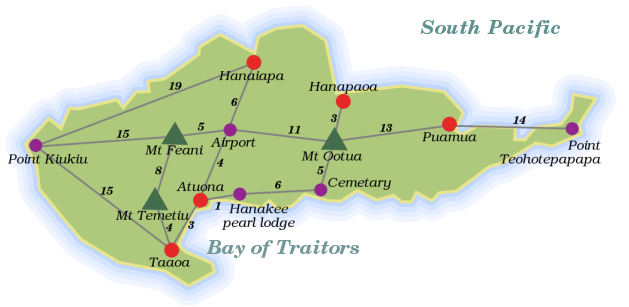
\includegraphics[width=\textwidth]{Hiva-Oa}} 
\smallskip
  
Szare linie oznaczają drogi, a znajdujące się obok nich numery informują, jaka jest długość tych dróg. Wyobraź sobie, że potrzebujesz programu znajdującego najkrótszą drogę między dwoma punktami na Hiva Oa. Jak się do tego zabrać? Pomyśl o tym przez chwilę.


Hej. Nie uciekaj do następnego rozdziału, tylko naprawdę spróbuj wymyślić jakieś sposoby na rozwiązanie tego zadania i zastanów się, jakie problemy możesz przy tym napotkać. Czytając techniczną książkę bardzo łatwo jest tylko rzucić okiem na tekst, pokiwać głową z uznaniem i od razu zapomnieć, co się przeczytało. Jeśli jednak naprawdę wysilisz się, aby rozwiązać problem, stanie się on \emph{Twoim} problemem i jego rozwiązanie będzie Ci bliższe.



\begin{center}
• • • • •
\end{center}

  
Pierwszym aspektem tej kwestii jest reprezentacja danych. Informacje przedstawione na obrazku dla komputera są mało przydatne. Moglibyśmy spróbować napisać program wydobywający informacje z mapy, ale byłoby to bardzo skomplikowane zadanie. Gdybyśmy mieli do zinterpretowania 20 tysięcy takich map, to pewnie byśmy napisali taki program, ale w tym przypadku zinterpretujemy mapę sami i zdobyte informacje przedstawimy w bardziej zrozumiały dla komputera sposób.

  
Co program powinien wiedzieć? Musi mieć możliwość sprawdzania, które miejsca są ze sobą połączone i jaką długość mają łączące je drogi. Miejsca i~drogi na tej wyspie tworzą tzw. \textbf{graf}\index{graf} (jest to pojęcie matematyczne). Grafy można przechowywać na wiele sposobów. Jednym z najprostszych z nich jest utworzenie tablicy obiektów drogowych zawierających własności określające nazwy punktów końcowych i długość…

  
\begin{verbatim} 
var roads = [{point1: "Point Kiukiu", point2: "Hanaiapa", length: 19},
             {point1: "Point Kiukiu", point2: "Mt Feani", length: 15}
             /* itd. */];
 \end{verbatim}
  
Jednak program szukając drogi bardzo często będzie potrzebował listy wszystkich dróg zaczynających się w określonym miejscu, podobnie jak osoba stojąca na rozdrożu i szukająca drogowskazu „Hanaiapa: 19km, Mount Feani: 15km”. Byłoby fajnie, gdyby dało się to zrobić łatwo i szybko.

  
Mając taką reprezentację, jak powyższa za każdym razem, gdy potrzebujemy takiej „drogowskazowej” listy, musimy przeglądać całą listę dróg, aby wybrać odpowiednie. Lepszym rozwiązaniem byłoby zapisanie tej listy bezpośrednio. Możemy np. użyć obiektu wiążącego nazwy miejsc z listami drogowskazów:

  
\begin{verbatim} 
var roads = {"Point Kiukiu": [{to: "Hanaiapa", distance: 19},
                              {to: "Mt Feani", distance: 15},
                              {to: "Taaoa", distance: 15}],
             "Taaoa": [/* itd. */]};
 \end{verbatim}
  
Mając taki obiekt, aby znaleźć drogi z Point Kiukiu, wystarczy zajrzeć do \texttt{roads["Point Kiukiu"]}.



\begin{center}
• • • • •
\end{center}

  
Jednak ta reprezentacja zawiera duplikaty informacji: droga między A i~B jest zaznaczona zarówno w A jak i B. Już pierwsza wersja wymagała sporo pisania, a ta wymaga jeszcze więcej.

  
Na szczęście możemy wykorzystać umiejętność komputera do wykonywania powtarzalnych czynności. Możemy określić drogi raz i wygenerować odpowiednią strukturę danych za pomocą komputera. Zaczniemy od zainicjowania pustego obiektu o nazwie \texttt{roads} i napisania funkcji \texttt{makeRoad}:

  
\begin{verbatim} 
var roads = {};
function makeRoad(from, to, length) {
  function addRoad(from, to) {
    if (!(from in roads))
      roads[from] = [];
    roads[from].push({to: to, distance: length});
  }
  addRoad(from, to);
  addRoad(to, from);
}
 \end{verbatim}
  
Elegancko, prawda? Zwróć uwagę, że w funkcji wewnętrznej \texttt{addRoad} użyte zostały parametry o takich samych nazwach (\texttt{from} i \texttt{to}), jak w funkcji zewnętrznej. Nie spowoduje to konfliktów, ponieważ wewnątrz funkcji \texttt{addRoad} nazwy te odnoszą się do parametrów funkcji \texttt{addRoad}, a poza nią — do do parametrów funkcji \texttt{makeRoad}.

  
Instrukcja \texttt{if} w funkcji \texttt{addRoad} sprawdza czy istnieje tablica miejsc związanych z lokalizacją określoną w \texttt{from}. Jeśli nie ma, dodaje pustą tablicę. Dzięki temu w następnym wierszu można przyjąć, że taka tablica istnieje i~bezpiecznie wstawić do niej nową drogę.

  
Teraz informacje z mapy wyglądają tak:

  
\begin{verbatim} 
makeRoad("Point Kiukiu", "Hanaiapa", 19);
makeRoad("Point Kiukiu", "Mt Feani", 15);
makeRoad("Point Kiukiu", "Taaoa", 15);
// ...
 \end{verbatim}


\begin{center}
• • • • •
\end{center}

  
\section*{Ćwiczenie 7.1}
\label{sec:7.1}
  
    
W powyższym opisie łańcuch \texttt{"Point Kiukiu"} nadal występuje trzy razy po kolei. Moglibyśmy nasz opis jeszcze bardziej skrócić, gdybyśmy zezwolili na określanie kilku dróg w jednym wierszu.

    
Napisz funkcję o nazwie \texttt{makeRoads} pobierającą dowolną nieparzystą liczbę argumentów. Pierwszy argument jest zawsze punktem początkowym dróg, a każda para argumentów znajdująca się za nim określa punkt końcowy i~długość drogi.

    
Nie duplikuj kodu funkcji \texttt{makeRoad}, tylko spraw, aby funkcja \texttt{makeRoads} wywoływała \texttt{makeRoad}.

  
[\hyperref[sol:7.1]{pokaż rozwiązanie}]
  


\begin{center}
• • • • •
\end{center}

  
Definiując kilka wygodnych operacji udało się nam znacznie skrócić nasz opis informacji o drogach. Można powiedzieć, że zwięźle wyraziliśmy te informacje poprzez rozszerzenie słownika.\index{język dziedzinowy} Zdefiniowanie „małego języka” jak ten jest często bardzo przydatną techniką — jeśli kiedykolwiek będziesz musiał wielokrotnie wpisywać ten sam kod,  postaraj się opracować słownik, który pozwoli Ci to skrócić.

  
Wpisywanie niepotrzebnego kodu jest nie tylko żmudne, ale i łatwo przy tym popełnić błąd, ponieważ przy wykonywaniu czynności niewymagających myślenia ludzie często popełniają błędy. Ponadto wielokrotnie powtarzający się kod trudno jest modyfikować, ponieważ jeśli jakaś struktura powtarza się w kodzie setki razy, trzeba wprowadzić zmiany w setkach miejsc. 



\begin{center}
• • • • •
\end{center}

  
Jeśli wykonałeś wszystkie wcześniejsze fragmenty kodu, powinieneś teraz mieć zmienną o nazwie \texttt{roads} zawierającą wszystkie drogi na wyspie. Gdy będziemy potrzebować dróg zaczynających się w wybranym miejscu, wystarczy, że napiszemy \texttt{roads[place]}. Jeżeli jednak ktoś popełni błąd przy wpisywaniu nazwy miejsca, co jest całkiem możliwe biorąc pod uwagę, jak one wyglądają, zamiast spodziewanej tablicy otrzyma wartość \texttt{undefined} i wystąpią różne dziwne błędy. Dlatego napiszemy funkcję, która będzie pobierała tablice dróg i krzyczała na nas, gdy podamy nieznaną nazwę miejsca:

  
\begin{verbatim} 
function roadsFrom(place) {
  var found = roads[place];
  if (found == undefined)
    throw new Error("Nie znaleziono miejsca o nazwie '" + place + "'.");
  else
    return found;
}

show(roadsFrom("Puamua"));
// → [{to:	"Mt Ootua", distance: 13}, 
//    {to: "Point Teohotepapapa", distance: 14}]
\end{verbatim}


\begin{center}
• • • • •
\end{center}

  
Oto pierwsza próba napisania algorytmu \textbf{wyszukiwania drogi}, tzw. metoda hazardzisty (ang. gambler’s method):

  
\begin{verbatim} 
function gamblerPath(from, to) {
  function randomInteger(below) {
    return Math.floor(Math.random() * below);
  }
  function randomDirection(from) {
    var options = roadsFrom(from);
    return options[randomInteger(options.length)].to;
  }

  var path = [];
  while (true) {
    path.push(from);
    if (from == to)
      break;
    from = randomDirection(from);
  }
  return path;
}

show(gamblerPath("Hanaiapa", "Mt Feani"));
// → ["Hanaiapa", "Point Kiukiu", "Taaoa", "Point Kiukiu", "Mt Feani"]
\end{verbatim}
  
Na każdym rozgałęzieniu dróg hazardzista rzuca kostką, aby zdecydować, w którą stronę pójść. Jeśli wyjdzie mu, że powinien wrócić tam, skąd przyszedł, to również to zrobi. W końcu dotrze w miejsce docelowe, ponieważ wszystkie miejsca na wyspie są ze sobą połączone.

  
Najmniej zrozumiały wiersz kodu w tym przykładzie to zapewne ten zawierający instrukcję \texttt{Math.random}\index{Math.random}. Funkcja ta zwraca pseudolosową liczbę\footnote{Komputery to maszyny deterministyczne: zawsze reagują w ten sam sposób na dane wejściowe, przez co nie mogą generować rzeczywiście losowych danych. Dlatego musimy polegać na szeregach liczb, które wyglądają na losowe, a w rzeczywistości są wynikiem skomplikowanych deterministycznych obliczeń.} z~przedziału 0-1. Wywołaj ją kilka razy w konsoli, a w większości przypadków za każdym razem otrzymasz inną liczbę. Funkcja \texttt{randomInteger} mnoży tę liczbę przez otrzymany argument i zaokrągla wynik w dół za pomocą funkcji \texttt{Math.floor}. Dzięki temu instrukcja \texttt{randomInteger(3)} może zwrócić liczby \texttt{0}, \texttt{1} oraz \texttt{2}.



\begin{center}
• • • • •
\end{center}

  
Metoda hazardzisty jest dobra dla tych, którzy brzydzą się uporządkowaną strukturą i nie lubią planować oraz ciągle szukają przygód. My jednak mieliśmy napisać program znajdujący \emph{najkrótszą} drogę między dwoma miejscami, a więc musimy bardziej się postarać.

  
Bardzo proste podejście do rozwiązania tego problemu nosi nazwę „generuj i sprawdzaj”\index{generuj i sprawdzaj}. Polega ono na:

  \begin{enumerate}
    \item wygenerowaniu wszystkich możliwych tras,
    \item i wybraniu z otrzymanego zbioru najkrótszej trasy łączącej punkt początkowy z końcowym.
  \end{enumerate}
  
Realizacja drugiego kroku jest łatwa. Natomiast pierwszy krok może sprawiać problemy. Jeśli dopuści się trasy z kołami, to będzie nieskończona liczba tras. Oczywiście trasy z kołami nie mogą być najkrótsze dokądkolwiek, a dodatkowo można odrzucić trasy nie zaczynające się w punkcie początkowym. Dla małego grafu, jak Hiva Oa powinno być możliwe wygenerowanie wszystkich niecyklicznych (wolnych od kół) tras zaczynających się w określonym punkcie.



\begin{center}
• • • • •
\end{center}

  
Wcześniej jednak będziemy potrzebować pewnych nowych narzędzi. Pierwszym z nich jest funkcja o nazwie \texttt{member} służąca do sprawdzania, czy wybrany element znajduje się w tablicy. Trasa będzie przechowywana jako tablica nazw i docierając w nowe miejsce algorytm będzie wywoływał funkcję \texttt{member}, aby sprawdzić czy już w tym miejscu był. Może to wyglądać następująco:

  
\begin{verbatim} 
function member(array, value) {
  var found = false;
  forEach(array, function(element) {
    if (element === value)
      found = true;
  });
  return found;
}

print(member([6, 7, "Bordeaux"], 7));
// → true
\end{verbatim}
  
Teraz jednak przeglądana będzie cała tablica, nawet jeśli wartość zostanie znaleziona natychmiast na pierwszej pozycji. Co za marnotrawstwo. W pętli \texttt{for} można zakończyć iterację za pomocą instrukcji \texttt{break}, ale w pętli \texttt{forEach} tak się nie da, ponieważ treść pętli jest funkcją, a instrukcja \texttt{break} nie służy do wychodzenia z funkcji. Jednym z możliwych rozwiązań jest dostosowanie \texttt{forEach}, aby rozpoznawała określony typ wyjątków jako sygnał do przerwania.

  
\begin{verbatim} 
var Break = {toString: function() {return "Break";}};

function forEach(array, action) {
  try {
    for (var i = 0; i < array.length; i++)
      action(array[i]);
  }
  catch (exception) {
    if (exception != Break)
      throw exception;
  }
}
 \end{verbatim}
  
Teraz gdy funkcja \texttt{action} zgłosi wyjątek \texttt{Break}, funkcja \texttt{forEach} go przechwyci i przerwie iterację. Obiekt przechowywany w zmiennej \texttt{Break} jest używany wyłącznie w celach porównawczych. Własność \texttt{toString} dodałem mu po to, aby ułatwić zorientowanie się, co za dziwną wartość otrzymaliśmy, gdy jakimś cudem wyjątek \texttt{Break} pojawi się poza \texttt{forEach}.



\begin{center}
• • • • •
\end{center}

  
Możliwość wyjścia z pętli \texttt{forEach} może być bardzo przydatna, ale w~przypadku funkcji \texttt{member} wynik jest raczej nieładny, ponieważ trzeba zapisać wynik, a następnie go zwrócić. Możemy dodać jeszcze jeden rodzaj wyjątku, \texttt{Return}, z własnością \texttt{value} i zwracać tę wartość w \texttt{forEach}, gdy taki wyjątek zostanie zgłoszony, ale to by było bardzo przypadkowe i nieeleganckie rozwiązanie. Tak naprawdę potrzebujemy nowej funkcji wyższego rzędu o nazwie \texttt{any} (lub czasami \texttt{some}). Oto jej implementacja:

  
\begin{verbatim} 
function any(test, array) {
  for (var i = 0; i < array.length; i++) {
    var found = test(array[i]);
    if (found)
      return found;
  }
  return false;
}

function member(array, value) {
  return any(partial(op["==="], value), array);
}

print(member(["Strach", "Obrzydzenie"], "Wyparcie"));
// → false
\end{verbatim}
  
Funkcja \texttt{any} przegląda elementy tablicy od lewej i wykonuje na nich funkcję testową. Gdy funkcja testowa zwróci wartość oznaczającą prawdę, funkcja \texttt{any}\index{any} zwraca tę wartość. Jeśli wartość oznaczająca prawdę nie zostanie znaleziona, następuje zwrot wartości \texttt{false}. Wywołanie \texttt{any(test, array)} jest mniej więcej równoważne z wyrażeniem \texttt{test(array[0]) || test(array[1]) ||…} itd.



\begin{center}
• • • • •
\end{center}

  
Podobnie jak operator \texttt{\&\&} ma uzupełnienie w postaci operatora \texttt{||}, tak funkcja \texttt{any} ma uzupełnienie w postaci funkcji \texttt{every}\index{every}

  
\begin{verbatim} 
function every(test, array) {
  for (var i = 0; i < array.length; i++) {
    var found = test(array[i]);
    if (!found)
      return found;
  }
  return true;
}

show(every(partial(op["!="], 0), [1, 2, -1]));
// → true
\end{verbatim}


\begin{center}
• • • • •
\end{center}

  
Kolejna funkcja, jakiej będziemy potrzebować to \texttt{flatten}. Będzie pobierała tablicę tablic i wstawiała elementy tych tablic do jednej dużej tablicy.

  
\begin{verbatim} 
  function flatten(arrays) {
    var result = [];
    forEach(arrays, function (array) {
      forEach(array, function (element){result.push(element);});
    });
    return result;
  }
 \end{verbatim}
  
To samo można by było zrobić przy użyciu metody \texttt{concat} i jakiegoś rodzaju funkcji \texttt{reduce}, ale takie rozwiązanie byłoby mniej wydajne. Podobnie jak wielokrotne łączenie łańcuchów jest wolniejsze od umieszczenia fragmentów w tablicy i wywołanie funkcji \texttt{join}, także wielokrotne łączenie tablic powoduje powstanie niepotrzebnych pośrednich wartości tablicowych.



\begin{center}
• • • • •
\end{center}

  
\section*{Ćwiczenie 7.2}
\label{sec:7.2}
  
    
Przed rozpoczęciem generowania dróg potrzebujemy jeszcze jednej funkcji wyższego rzędu. Jest to funkcja \texttt{filter}\index{filter}. Podobnie jak \texttt{map} funkcja ta jako argumenty pobiera funkcję oraz tablicę i tworzy nową tablicę, tylko zamiast zapisywać w tej nowej tablicy wyniki wykonania funkcji z argumentu na tablicy z argumentu, zwraca tablicę zawierającą tylko te wartości ze starej tablicy, dla których funkcja z argumentu zwróciła wartość oznaczającą prawdę. Poniżej znajduje się kod implementacji tej funkcji.

  
[\hyperref[sol:7.2]{pokaż rozwiązanie}]
  


\begin{center}
• • • • •
\end{center}

  
Wyobraź sobie, jak mógłby wyglądać algorytm generowania tras ― zaczynałby działanie od miejsca początkowego i generował trasy dla każdej drogi wychodzącej z tego miejsca. Na końcu każdej z tych dróg generowałby kolejne trasy. Nie podążałby tylko jedną drogą, ale rozgałęziałby się. Z tego powodu naturalnym sposobem na jego realizację jest rekurencja\index{rekurencja}.

  
\begin{verbatim} 
function possibleRoutes(from, to) {
  function findRoutes(route) {
    function notVisited(road) {
      return !member(route.places, road.to);
    }
    function continueRoute(road) {
      return findRoutes({places: route.places.concat([road.to]),
                         length: route.length + road.distance});
    }

    var end = route.places[route.places.length - 1];
    if (end == to)
      return [route];
    else
      return flatten(map(continueRoute, filter(notVisited,
                                               roadsFrom(end))));
  }
  return findRoutes({places: [from], length: 0});
}

show(possibleRoutes("Point Teohotepapapa", "Point Kiukiu").length);
// → 11
show(possibleRoutes("Hanapaoa", "Mt Ootua"));
// → [{places: ["Hanapaoa", "Mt Ootua"], length: 2}]
\end{verbatim}
  
Ta funkcja zwraca tablicę obiektów tras, z których każdy zawiera tablicę miejsc, przez które dana trasa przechodzi oraz długość. Funkcja \texttt{findRoutes} rekurencyjnie kontynuuje trasę zwracając tablicę zawierającą każde możliwe rozszerzenie tej trasy. Gdy koniec trasy jest miejscem, do którego chcemy dotrzeć, zwraca tę trasę, ponieważ kontynuowanie poza to miejsce byłoby bezcelowe. Jeśli jest to inne miejsce, musimy kontynuować. Najtrudniejszy do rozszyfrowania jest wiersz kodu zawierający wywołania funkcji \texttt{flatten}/\texttt{map}/\texttt{filter}. Można go odczytać tak: „Weź wszystkie drogi wychodzące z bieżącej lokalizacji, odrzuć te, które prowadzą do już odwiedzonych przez tę trasę miejsc. Kontynuuj podążanie każdą z tych dróg, aby otrzymać tablicę ukończonych tras dla każdej z nich, a następnie umieść te wszystkie trasy w jednej wielkiej tablicy, która zostanie zwrócona”.

  
W tym wierszu dużo się dzieje. Dlatego właśnie pomocne są dobre abstrakcje: dzięki nim można wyrażać skomplikowane działania bez potrzeby pisania całych ekranów kodu.

  
Czy ta funkcja nie jest nieskończoną rekurencją, biorąc pod uwagę, że ciągle wywołuje samą siebie (poprzez funkcję \texttt{continueRoute})? Nie, w pewnym momencie wszystkie wychodzące drogi dojdą do miejsc, przez które trasa już przeszła i wynikiem funkcji \texttt{filter} będzie pusta tablica. Wynikiem mapowania pustej tablicy będzie pusta tablica, której spłaszczenie (flatten) również zwróci pustą tablicę. A więc wywołanie funkcji \texttt{findRoutes} na ślepym zaułku spowoduje powstanie pustej tablicy, która oznacza, że „nie ma możliwości kontynuowania tej trasy”.

  
Zwróć uwagę, że miejsca są dołączane do tras za pomocą metody \texttt{concat}\index{concat}, a nie \texttt{push}\index{push}. Metoda \texttt{concat} tworzy nową tablicę, podczas gdy \texttt{push} modyfikuje istniejącą. Jako że funkcja może z jednej częściowej trasy rozgałęzić się na kilka tras, nie możemy modyfikować tablicy reprezentującej oryginalną trasę, ponieważ tablica ta jest potrzebna kilka razy.



\begin{center}
• • • • •
\end{center}

  
\section*{Ćwiczenie 7.3}
\label{sec:7.3}
  
    
Mając wszystkie możliwe trasy możemy spróbować znaleźć najkrótszą. Napisz funkcję o nazwie \texttt{shortestRoute}, która popdobnie jak \texttt{possibleRoutes}, jako argumenty pobiera nazwy punktów początkowego i końcowego. Niech zwraca jeden obiekt trasy typu tworzonego przez funkcję \texttt{possibleRoutes}.

  
[\hyperref[sol:7.3]{pokaż rozwiązanie}]
  


\begin{center}
• • • • •
\end{center}

  
Sprawdźmy, jaką trasę nasz algorytm znajdzie między Point Kiukiu i~Point Teohotepapapa…

  
\begin{verbatim} 
show(shortestRoute("Point Kiukiu", "Point Teohotepapapa").places);
// → ["Point Kiukiu", "Taaoa", "Atuona", "Hanakee pearl lodge", 
//    "Cemetery", "Mt Ootua", "Puamua", "Point Teohotepapapa"]
\end{verbatim}


\begin{center}
• • • • •
\end{center}

  
Dla takiej małej wyspy, jak Hiva Oa wygenerowanie wszystkich możliwych tras nie wymaga dużo pracy. Jeśli jednak spróbujesz to samo zrobić dla szczegółowej mapy np. Belgii, to zajmie Ci to niesłychanie dużo czasu i pamięci komputerowej. A jednak zapewne nie raz widziałeś internetowe narzędzia do planowania podróży. Są one w stanie wskazać mniej więcej najlepszą trasę w~gigantycznej sieci dróg w ciągu zaledwie kilku sekund. Jak to robią?

  
Jeśli uważnie czytałeś, to mogłeś zauważyć, że nie trzeba generować wszystkich tras do samego końca. Jeśli zaczniemy porównywać trasy \emph{podczas} ich budowania, możemy uniknąć tworzenia tego wielkiego zbioru tras i po znalezieniu pierwszej trasy prowadzącej do celu możemy zaniechać badania tras, które są dłuższe od już znalezionej.



\begin{center}
• • • • •
\end{center}

  
Aby to sprawdzić, użyjemy jako mapy siatki o wymiarach 20 na 20:

\bigskip 
\centerline{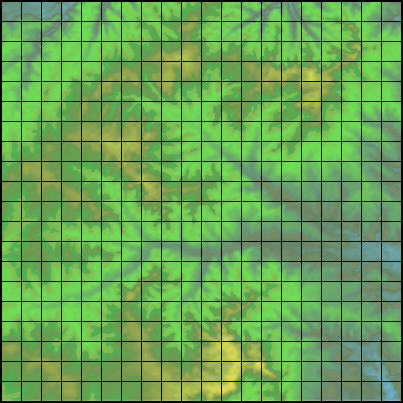
\includegraphics[width=\textwidth]{height}} 
\smallskip
  
Jest to mapa topograficzna górzystego obszaru. Żółte punkty to szczyty, a niebieskie to doliny. Obszar jest podzielony na prostokąty o rozmiarze 100 metrów. Mamy do dyspozycji funkcję o nazwie \texttt{heightAt}, która zwraca wysokość w metrach dowolnego prostokąta na mapie, przy czym prostokąty są reprezentowane jako obiekty z własnościami \texttt{x} i \texttt{y}.

  
\begin{verbatim} 
print(heightAt({x: 0, y: 0}));
// → 111
print(heightAt({x: 11, y: 18}));
// → 448
\end{verbatim}


\begin{center}
• • • • •
\end{center}

  
Chcemy przejść przez ten obszar pieszo rozpoczynając wędrówkę w lewym górnym rogu, a kończąc w prawym dolnym. Do siatki można podejść jak do grafu. Każdy prostokąt jest węzłem połączonym z prostokątami, które go otaczają.

  
Nie lubimy marnować energii i dlatego chcielibyśmy znaleźć jak najłatwiejszą trasę. Wchodzenie pod górę jest o wiele trudniejsze niż schodzenie w dół, a schodzenie w dół jest trudniejsze niż marsz po poziomym podłożu\footnote{Naprawdę tak jest.}. Ta funkcja oblicza liczbę „metrów ważonych” między dwoma przylegającymi do siebie prostokątami. Wynik ten określa jak bardzo się zmęczymy przechodząc z jednego do drugiego prostokąta. Wędrówka pod górę liczy się jako dwa razy cięższa od schodzenia w dół.

  
\begin{verbatim} 
function weightedDistance(pointA, pointB) {
  var heightDifference = heightAt(pointB) - heightAt(pointA);
  var climbFactor = (heightDifference < 0 ? 1 : 2);
  var flatDistance = (pointA.x == pointB.x || pointA.y == pointB.y ? 100 : 141);
  return flatDistance + climbFactor * Math.abs(heightDifference);
}
 \end{verbatim}
  
Zwróć uwagę na obliczenia \texttt{flatDistance}. Jeśli dwa punkty znajdują się w tym samym wierszu lub tej samej kolumnie, to znaczy, że znajdują się obok siebie i odległość między nimi wynosi sto metrów. W przeciwnym razie można przyjąć, że prostokąty sąsiadują po przekątnej, a odległość po przekątnej między dwoma prostokątami o takim rozmiarze wynosi sto razy pierwiastek kwadratowy z dwóch, czyli w przybliżeniu \texttt{141}. Funkcja ta nie może być wywoływana dla kwadratów, które się ze sobą nie stykają. (Mogłaby to dokładnie sprawdzać, ale jest zbyt leniwa.)



\begin{center}
• • • • •
\end{center}

  
Punkty na mapie są reprezentowane przez obiekty zawierające własności \texttt{x} i \texttt{y}. Poniżej znajdują się trzy funkcje przydatne w pracy z takimi obiektami:

  
\begin{verbatim} 
function point(x, y) {
  return {x: x, y: y};
}

function addPoints(a, b) {
  return point(a.x + b.x, a.y + b.y);
}

function samePoint(a, b) {
  return a.x == b.x && a.y == b.y;
}

show(samePoint(addPoints(point(10, 10), point(4, -2)),
               point(14, 8)));
// → true
\end{verbatim}


\begin{center}
• • • • •
\end{center}

  
\section*{Ćwiczenie 7.4}
\label{sec:7.4}
  
    
Aby znaleźć trasy na tej mapie, znowu potrzebujemy funkcji do tworzenia „drogowskazów” czyli list kierunków, w których można pójść z określonego miejsca. Napisz funkcję o nazwie \texttt{possibleDirections} pobierającą jako argument obiekt punktu i zwracającą tablicę pobliskich punktów. Możemy przechodzić tylko do sąsiadujących punktów, zarówno na wprost jak i po ukosie, a więc każdy kwadrat może mieć maksymalnie ośmiu sąsiadów. Uważaj, aby nie zwracać kwadratów leżących poza mapą. Dla nas w tym przypadku krawędź mapy oznacza koniec świata.

  
[\hyperref[sol:7.4]{pokaż rozwiązanie}]
  


\begin{center}
• • • • •
\end{center}

  
Aby znaleźć trasę na tej mapie i uniknąć wyłączenia programu przez przeglądarkę z powodu zbyt długiego czasu działania, musimy skończyć z~amatorskimi rozwiązaniami i zaimplementować poważny algorytm. Problemy tego typu były już wielokrotnie analizowane, czego wynikiem jest wiele różnych rozwiązań (niektóre genialne inne bezużyteczne). Jednym z najpopularniejszych i najbardziej wydajnych jest tzw. \textbf{A*}\index{A*} (wym. \textbf{A-star}). Do końca tego rozdziału będziemy zajmować się implementowaniem algorytmu A* do znajdowania tras na naszej mapie.

  
Zanim przejdę do objaśniania samego algorytmu, kilka słów o rodzaju problemów, jakie można za jego pomocą rozwiązać. Problem ze znajdowaniem tras w grafach polega na tym, że jeśli graf jest duży, to zawiera bardzo dużo potencjalnych tras. Nasz algorytm znajdowania tras na wyspie Hiva Oa wykazał, że gdy graf jest niewielki, to wystarczy uważać, aby ścieżki nie przechodziły więcej niż raz przez jeden punkt. Jednak w naszej nowej mapie to nie wystarczy.

  
Sedno problemu tkwi w tym, że jest zbyt wiele możliwości pójścia w niewłaściwym kierunku. Jeśli nie znajdziemy sposobu na pokierowanie naszych poszukiwań ścieżek w kierunku celu, podczas wybierania kierunku kontynuacji poszukiwań będzie istniało większe ryzyko wyboru niewłaściwego kierunku niż szansa na wybór odpowiedniego. Jeśli w ten sposób będziemy generować ścieżki, otrzymamy ich ogromną ilość i nawet jeśli któraś z nich doprowadzi nas do punktu docelowego, to i tak nie będziemy mieć pewności, że będzie to najkrótsza droga.

  
Dlatego w pierwszej kolejności powinniśmy badać tylko te kierunki, które dają szansę na dojście do celu. W takiej siatce, jak nasza mapa ścieżkę można z grubsza ocenić sprawdzając jej długość i odległość jej końca od punktu docelowego. Sumując długość ścieżki i szacunkową odległość, jaka pozostała do przejścia można ocenić, które ścieżki są obiecujące. Jeśli będziemy najpierw badać obiecujące ścieżki, zmarnujemy mniej czasu na bezużyteczne.



\begin{center}
• • • • •
\end{center}

  
Ale to wciąż za mało. Gdyby nasza mapa przedstawiała idealnie płaski teren, ścieżka wyglądająca na obiecującą prawie zawsze byłaby najlepsza i moglibyśmy użyć powyższej metody do osiągnięcia naszego celu. Ale na naszej mapie mamy wzgórza i zbocza gór blokujące ścieżki, przez co trudno z góry powiedzieć, który kierunek jest najlepszą ścieżką. Przez to nadal jesteśmy zmuszeni badać zbyt dużą liczbę ścieżek.

  
Aby to zmienić, możemy sprytnie wykorzystać fakt, że zawsze najpierw sprawdzamy najbardziej obiecującą ścieżkę. Gdy dowiemy się, że ścieżka A jest najlepszą drogą do punktu X, możemy to zapamiętać. Gdy później ścieżka B również dojdzie do punktu X, będziemy wiedzieć, że to nie jest najlepsza droga i nie będziemy musieli dalej jej badać. W ten sposób można zaoszczędzić programowi konieczności tworzenia wielu niepotrzebnych ścieżek.



\begin{center}
• • • • •
\end{center}

  
Zasada działania interesującego nas algorytmu jest następująca…

  
Są dwie informacje, które należy cały czas śledzić. Pierwsza z nich nazywa się listą otwartą (ang. open list) i zawiera częściowe trasy, które trzeba jeszcze zbadać. Każda trasa ma punktację obliczoną poprzez zsumowanie jej długości z szacowaną odległością od celu. Szacunek zawsze musi być optymistyczny, tzn. nigdy nie należy przeszacowywać odległości. Druga informacja to zbiór węzłów, które widzieliśmy z najkrótszymi częściowymi ścieżkami, po których do nich dotarliśmy. Zbiór ten nazwiemy listą osiągniętych celów (ang. reached list). Zaczynamy od dodania do listy otwartej trasy zawierającej tylko węzeł początkowy i zapisania go na liście osiągniętych celów.

  
Następnie, dopóki są węzły na liście otwartej, pobieramy węzeł o najniższej (najlepszej) punktacji i znajdujemy drogi kontynuacji (wywołując funkcję \texttt{possibleDirections}). Dla każdego zwróconego węzła tworzymy nową trasę dodając go do oryginalnej trasy i dostosowując jej długość za pomocą funkcji \texttt{weightedDistance}. Punkt końcowy każdej z tych nowych tras jest następnie szukany na liście osiągniętych celów.

  
Jeśli węzła nie ma jeszcze na tej liście, oznacza to że jeszcze nie mieliśmy z~nim do czynienia i dodajemy nową trasę do listy otwartej oraz zapisujemy to na liście osiągniętych celów. Jeśli \emph{widzieliśmy} węzeł wcześniej, porównujemy punktację nowej trasy z punktacją trasy na liście osiągniętych celów. Jeśli nowa trasa jest krótsza, zastępujemy nią istniejącą trasę. W przeciwnym razie odrzucamy nową trasę, ponieważ znamy już lepszą drogę do tego miejsca.

  
Czynności te powtarzamy aż trasa pobrana z listy otwartej będzie kończyć się w węźle docelowym, co oznacza, że znaleźliśmy trasę, albo aż lista otwarta zostanie wyczerpana, co będzie oznaczać, że nie ma drogi do tego miejsca. Na naszej mapie nie ma miejsc nie do przejścia, a więc zawsze znajdzie się trasa.

  
Skąd wiadomo, że pierwsza znaleziona pełna trasa pobrana z listy otwartej jest najkrótsza? Wiemy to dzięki temu, że do zbadania zawsze wybieramy tylko trasy o najniższej punktacji. Punktacja trasy składa się z jej długości plus \emph{optymistycznego} szacunku pozostałej długości. Oznacza to, że jeśli trasa ma najniższą punktację na liście otwartej, jest najlepszą drogą do swojego bieżącego punktu końcowego — nie ma możliwości, aby inna trasa później znalazła lepszą drogę do tego samego punktu, ponieważ gdyby było to możliwe, miałaby niższą punktację.



\begin{center}
• • • • •
\end{center}

  
Nie przejmuj się, jeśli to wszystko wydaje Ci się zagmatwane. W zrozumieniu takich algorytmów, jak ten bardzo pomaga skojarzenie ich z czymś, co się już wcześniej widziało. Ma się wówczas punkt odniesienia. Początkujący programiście są pozbawieni takiego punktu i dlatego trudno jest im się połapać. Po prostu uświadom sobie, że rozważania przedstawione w tym rozdziale dotyczą zaawansowanych zagadnień. Przeczytaj go w całości, a potem wróć do niego po przestudiowaniu reszty książki, jeśli będziesz mieć ochotę na małe wyzwanie.



\begin{center}
• • • • •
\end{center}

  
Obawiam się, że w jednym aspekcie algorytmu znowu będę musiał skorzystać z magicznych sztuczek. Lista otwarta musi być w stanie pomieścić dużą liczbę tras oraz szybko znajdować wśród nich trasy o najniższej punktacji. Przechowywanie ich w normalny sposób i przeszukiwanie tablicy byłoby o~wiele za wolne. Dlatego dam Ci do dyspozycji strukturę danych o nazwie kopiec binarny\index{kopiec binarny}. Kopce binarne tworzy się przy użyciu słowa \texttt{new}, podobnie jak obiekty \texttt{Date}, podając im jako argument funkcję służącą do „punktowania” swoich elementów. Powstały obiekt ma metody \texttt{push} i \texttt{pop}, podobnie jak tablice, z tym że \texttt{pop} zawsze zwraca element o najniższej punktacji, zamiast elementu, który został dodany jako ostatni.

  
\begin{verbatim} 
function identity(x) {
  return x;
}

var heap = new BinaryHeap(identity);
forEach([2, 4, 5, 1, 6, 3], function(number) {
  heap.push(number);
});
while (heap.size() > 0)
  show(heap.pop());
// → 1
// → 2
// → 3
// → 4
// → 5
// → 6
\end{verbatim}
  
W \hyperref[app:2]{dodatku 2} opisałem implementację tej struktury danych. Warto przeczytać. Najlepiej zrobić to po lekturze \hyperref[chap:8]{rozdziału 8}.



\begin{center}
• • • • •
\end{center}

  
Potrzeba wyciśnięcia maksimum wydajności ma jeszcze inny efekt. W~algorytmie dotyczącym wyspy Hiva Oa do przechowywania tras używano tablic lokalizacji, które podczas przedłużania kopiowano przy użyciu metody \texttt{concat}. Tym razem nie możemy pozwolić sobie na kopiowanie tablic, ponieważ liczba tras będzie o wiele większa. Zamiast tego do przechowywania tras będziemy używać „łańcuchów” obiektów. Każdy obiekt w łańcuchu ma pewne własności, jak punkt na mapie i długość trasy do tego miejsca, a także własność wskazującą na poprzedni obiekt w łańcuchu. Wygląda to mniej więcej tak:

  \bigskip 
 \centerline{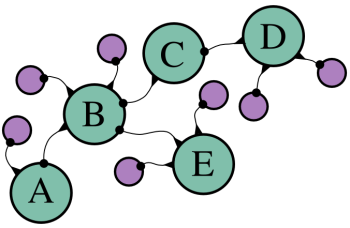
\includegraphics{objectchain}} 
 \smallskip
  
Zielone koła to istotne obiekty, a linie reprezentują własności ― końcówka z kropką wskazuje wartość własności. Obiekt \texttt{A} jest początkiem tej trasy. Obiekt \texttt{B} służy do budowy nowej trasy, która jest kontynuowana z punktu \texttt{A}. Ma własność, którą nazwiemy \texttt{from}, wskazującą rasę, na której bazuje. Jeśli później będziemy chcieli odtworzyć trasę, będziemy mogli pójść po tych własnościach, aby znaleźć wszystkie punkty, przez które trasa ta przechodziła. Zwróć uwagę, że punkt \texttt{B} należy do dwóch tras, z których jedna kończy się w~punkcie \texttt{D}, a druga w \texttt{E}. Gdy tras jest dużo, można w ten sposób zaoszczędzić dużo miejsca — każda nowa trasa wymaga tylko jednego nowego obiektu, ponieważ pozostałe dzieli z innymi trasami, które rozpoczęły się w~taki sam sposób.



\begin{center}
• • • • •
\end{center}

  
\section*{Ćwiczenie 7.5}
\label{sec:7.5}
  
    
Napisz funkcję o nazwie \texttt{estimatedDistance} optymistycznie szacującą odległość między dwoma punktami. Może nie brać pod uwagę danych dotyczących wysokości, czyli traktować mapę jako płaski teren. Pamiętaj, że poruszać możemy się tylko na wprost i po skosie oraz, że odległość na ukos między dwoma kwadratami wynosi \texttt{141}.

  
[\hyperref[sol:7.5]{pokaż rozwiązanie}]
  


\begin{center}
• • • • •
\end{center}

  
\section*{Ćwiczenie 7.6}
\label{sec:7.6}
  

Do przechowywania listy otwartej użyjemy kopca binarnego. A jaka struktura danych byłaby dobra dla listy osiągniętych celów? Będziemy w niej wyszukiwać trasy na podstawie par współrzędnych \texttt{x}, \texttt{y}. Najlepiej żeby to wyszukiwanie było szybkie. Napisz trzy funkcje, \texttt{makeReachedList}, \texttt{storeReached} oraz \texttt{findReached}. Pierwsza niech tworzy Twoją strukturę danych, druga niech pobiera listę osiągniętych celów, punkt oraz trasę i zapisuje w tej strukturze trasę, a trzecia niech pobiera listę celów osiągniętych oraz punkt i pobiera trasę albo zwraca wartość \texttt{undefined} oznaczającą, że dla danego punktu nie została znaleziona żadna trasa.

[\hyperref[sol:7.6]{pokaż rozwiązanie}]
  


\begin{center}
• • • • •
\end{center}

  
\index{hermetyzacja}Definiowanie typu struktury danych poprzez dostarczenie zbioru funkcji do tworzenia jej egzemplarzy i manipulowania nimi to bardzo przydatna technika. Umożliwia to oddzielenie kodu korzystającego z tej struktury od szczegółów implementacyjnych samej tej struktury. Zwróć uwagę, że bez względu na to, która z powyższych dwóch implementacji zostanie użyta, kod korzystający z listy celów osiągniętych działa dokładnie tak samo. Dla niego nie ma znaczenia, jakiego rodzaju obiekty są używane, dopóki otrzymuje takie wyniki, jakich potrzebuje.

  
Bardziej szczegółowo na ten temat piszę w \hyperref[chap:8]{rozdziale 8}, w którym nauczysz się tworzyć typy obiektowe, takie jak \texttt{BinaryHeap}, które tworzy się przy użyciu słowa kluczowego \texttt{new} i mają metody służące do manipulowania nimi.



\begin{center}
• • • • •
\end{center}

  
W końcu możemy napisać funkcję znajdującą ścieżki:

  
\begin{verbatim} 
function findRoute(from, to) {
  var open = new BinaryHeap(routeScore);
  var reached = makeReachedList();

  function routeScore(route) {
    if (route.score == undefined)
      route.score = estimatedDistance(route.point, to) +
                    route.length;
    return route.score;
  }
  function addOpenRoute(route) {
    open.push(route);
    storeReached(reached, route.point, route);
  }
  addOpenRoute({point: from, length: 0});

  while (open.size() > 0) {
    var route = open.pop();
    if (samePoint(route.point, to))
      return route;
    
    forEach(possibleDirections(route.point), function(direction) {
      var known = findReached(reached, direction);
      var newLength = route.length +
                      weightedDistance(route.point, direction);
      if (!known || known.length > newLength){
        if (known)
          open.remove(known);        
        addOpenRoute({point: direction,
                      from: route,
                      length: newLength});
      }
    });
  }
  return null;
}
 \end{verbatim}
  
Najpierw tworzone są potrzebne struktury danych — lista otwarta i lista osiągniętych celów. \texttt{routeScore} to funkcja punktująca przekazywana do kopca binarnego. Zwróć uwagę, że zapisuje swój wynik w obiekcie trasy, aby uniknąć konieczności jego wielokrotnego obliczania.

  
Funkcja pomocnicza \texttt{addOpenRoute} dodaje nową trasę do list otwartej i~osiągniętych celów. Zostaje natychmiast użyta do dodania początku trasy. Zauważ, że obiekty tras zawsze mają własności \texttt{point}, która zawiera punkt będący końcem trasy, i \texttt{length}, która zawiera bieżącą długość trasy. Trasy o długości większej niż jeden kwadrat mają też własność \texttt{from}, wskazującą poprzedni kwadrat.

  
Pętla \texttt{while}, zgodnie z opisem algorytmu, pobiera z listy otwartej trasę o~najniższej punktacji i sprawdza, czy doprowadzi nas ona do celu. Jeśli nie, musimy kontynuować przedłużając ją. Tym zajmuje się kod \texttt{forEach}. Szuka tego nowego punktu na liście osiągniętych celów. Jeśli go tam nie znajdzie lub znaleziony węzeł ma większą długość niż nowa trasa, tworzony jest nowy obiekt trasy, który zostaje dodany do list otwartej i osiągniętych celów, a~istniejąca trasa (jeśli jest) zostaje usunięta z listy otwartej.

  
A co jeśli trasy w \texttt{known} nie ma na liście otwartej? Musi być, ponieważ trasy z listy otwartej są usuwane tylko wtedy, gdy zostaje odkryte, że stanowią najbardziej optymalną drogę do celu. Jeśli spróbujemy usunąć z kopca binarnego wartość, której w nim nie ma, kopiec zgłosi wyjątek, a więc jeśli moje rozumowanie jest niepoprawne, podczas wykonywania funkcji zapewne zobaczymy wyjątek.

  
Gdy kod staje się na tyle skomplikowany, że zaczynasz mieć wątpliwości, co do niektórych jego części, dobrze jest dodać kilka testów zgłaszających wyjątki, aby wiedzieć, co jest nie tak. Dzięki temu ma się pewność, że nie „prześlizgnie” się żaden błąd, a gdy wystąpi usterka, będzie ją można od razu naprawić.



\begin{center}
• • • • •
\end{center}

  
Zwróć uwagę, że mimo iż w algorytmie tym nie użyto rekurencji, to i~tak przeglądane są wszystkie odgałęzienia. Lista otwarta pełni podobną rolę, jak stos wywołań funkcji w wersji z rekurencją rozwiązującej problem wyspy Hiva Oa, tzn. prowadzi rejestr ścieżek, które jeszcze trzeba zbadać. Każdy rekurencyjny algorytm można zapisać w sposób nierekurencyjny używając struktury danych do przechowywania „rzeczy, które jeszcze trzeba zrobić”.



\begin{center}
• • • • •
\end{center}

  
Pora wypróbować nasz program:

  
\begin{verbatim} 
var route = findRoute(point(0, 0), point(19, 19));
 \end{verbatim}
  
Jeśli wykonałeś wszystkie poprzednie fragmenty kodu i nie spowodowałeś w żadnym z nich błędu, powyższe wywołanie powinno zwrócić obiekt trasy (może to chwilę potrwać). Obiekt ten jest mało czytelny. Można to zmienić przy użyciu funkcji \texttt{showRoute} wyświetlającej trasę na mapie, jeśli konsola będzie wystarczająco duża.

  
\begin{verbatim} 
showRoute(route);
 \end{verbatim}
  
Do funkcji \texttt{showRoute} można także przekazywać kilka tras, co może być przydatne np. przy planowaniu wycieczki krajoznawczej, która musi zawierać piękny widok o współrzędnych \texttt{11}, \texttt{17}.

  
\begin{verbatim} 
showRoute(findRoute(point(0, 0), point(11, 17)),
          findRoute(point(11, 17), point(19, 19)));
 \end{verbatim}


\begin{center}
• • • • •
\end{center}

  
Różne wersje algorytmu znajdowania\index{wyszukiwanie} optymalnej trasy na grafie mogą być zastosowane do różnych problemów, które wcale nie muszą być związane z szukaniem fizycznych dróg. Na przykład program, którego zadaniem jest upakowanie jak największej liczby klocków w ograniczonej przestrzeni może badać różne „trasy” otrzymywane poprzez umieszczenie określonego klocka w określonym miejscu. Ścieżki kończące się zbyt małą ilością miejsca dla ostatnich klocków są ślepymi zaułkami, a ścieżki, w których mieszczą się wszystkie klocki są rozwiązaniami.

\chapter{Programowanie obiektowe}
\label{chap:8}

Na początku lat 90. w branży programistycznej powstało zamieszanie spowodowane programowaniem obiektowym\index{programowanie obiektowe}. Większość zasad tej techniki nie była żadną nowością, ale osiągnęła ona na tyle dużą popularność, że w końcu nabrała pędu i zaczęła robić się modna. Pisano książki na jej temat, przeprowadzano kursy oraz tworzono nowe obiektowe języki programowania. Nagle wszyscy zaczęli wychwalać pod niebiosa zalety obiektowości i z entuzjazmem używać jej do rozwiązywania wszystkich możliwych problemów. Wyglądało to tak, jakby niektórzy byli przekonani, że w końcu odkryli \emph{prawidłowy sposób pisania programów}.

  
Jest to dość typowe... Gdy coś jest bardzo skomplikowane, ludzie zawsze szukają jakiegoś magicznego rozwiązania. I gdy pojawi się cos, co tak wygląda, od razu zyskuje potężną rzeszę oddanych wielbicieli. Do dziś dla wielu programistów obiektowość (albo ich wyobrażenie obiektowości) jest świętością. Dla nich program, który nie jest „prawdziwie obiektowy” (cokolwiek to znaczy), to słaby program. 

  
Niemniej jednak niewiele jest przejściowych mód, które przetrwałyby tak długo. Sukces obiektowości można w dużym stopniu tłumaczyć tym, że jest oparta na solidnych podstawach. W tym rozdziale znajduje się opis właśnie tych podwalin obiektowości oraz ich adaptacja w JavaScripcie. Chcę też podkreślić, że w poprzednich akapitach nie chciałem zdyskredytować obiektowości jako takiej. Moją intencją było tylko ostrzec Cię przed nadmiernym przywiązywaniem się do tej metodologii programowania.



\begin{center}
• • • • •
\end{center}

  
Jak nazwa wskazuje, \textbf{programowanie obiektowe} polega na używaniu obiektów. Do tej pory używaliśmy ich do luźnego grupowania wartości, dodając i usuwając z nich dane, gdy tak się nam podobało. W programowaniu obiektowym obiekty są traktowane jak małe samodzielne światy, a~świat zewnętrzny może się z nimi kontaktować tylko poprzez niewielki ściśle zdefiniowany interfejs\index{interfejs}, będący zestawem metod i własności. Przykładem tego jest lista osiągniętych celów, której używaliśmy na końcu \hyperref[chap:7]{rozdziału 7}. Do posługiwania się nią używaliśmy tylko trzech funkcji: \texttt{makeReachedList}, \texttt{storeReached} oraz \texttt{findReached}. Te trzy funkcje stanowią interfejs tego typu obiektów.

  
To samo dotyczy obiektów \texttt{Date}, \texttt{Error} i \texttt{BinaryHeap}. Zamiast zwykłych funkcji do pracy z obiektami, do dyspozycji mamy słowo kluczowe \texttt{new} do tworzenia obiektów, które wraz z pewną liczbą metod i własności stanowi ich interfejs.



\begin{center}
• • • • •
\end{center}

  
Jednym ze sposobów na dodanie metod do obiektów jest po prostu dołączenie do nich funkcji.

  
\begin{verbatim} 
var rabbit = {};
rabbit.speak = function(line) {
  print("Królik powiedział „", line, "”");
};

rabbit.speak("Teraz Ty pytasz mnie.");
// → Królik powiedział „Teraz Ty pytasz mnie.”
\end{verbatim}
  
W większości przypadków \textbf{metoda} musi wiedzieć, \emph{na czym} ma działać. Na przykład, jeśli byłoby kilka królików, metoda \texttt{speak} musiałaby wskazywać, który królik ma mówić. Do tego służy specjalna zmienna o nazwie \texttt{this}\index{this}, która jest zawsze dostępna w wywołaniu funkcji, a jeśli funkcja jest wywoływana jako metoda, wskazuje odpowiedni obiekt. Funkcja nazywa się metodą, gdy należy do obiektu i jest z niego wywoływana, np. \texttt{object.method()}.

  
\begin{verbatim} 
function speak(line) {
  print("Pewien ", this.adjective, " królik mówi „", line, "”");
}
var whiteRabbit = {adjective: "biały", speak: speak};
var fatRabbit = {adjective: "gruby", speak: speak};

whiteRabbit.speak("Na moje uszy i wąsy, która to już godzina!");
// → Pewien biały królik mówi „Na moje uszy i wąsy, która to już godzina!”
fatRabbit.speak("Nie pogardziłbym jakąś małą marchewką.");
// → Pewien gruby królik mówi „Nie pogardziłbym jakąś małą marchewką.”
\end{verbatim}


\begin{center}
• • • • •
\end{center}

  
Teraz mogę wyjaśnić do czego służy ten tajemniczy pierwszy argument metody \texttt{apply}\index{apply}, któremu zawsze przypisywaliśmy wartość \texttt{null} w \hyperref[chap:6]{rozdziale 6}. Przy jego użyciu można określić obiekt, do którego ma zostać zastosowana funkcja. W przypadku funkcji niebędących metodami argument ten jest niepotrzebny i dlatego nadawaliśmy mu wartość \texttt{null}.

  
\begin{verbatim} 
speak.apply(fatRabbit, ["Pycha."]);
// → Pewien gruby królik mówi „Pycha.”
\end{verbatim}
  
Funkcje również mają metodę \texttt{call}\index{call}, która jest podobna do \texttt{apply}, ale przyjmuje argumenty dla funkcji oddzielnie, zamiast w tablicy:

  
\begin{verbatim} 
speak.call(fatRabbit, "Burp.");
// → Pewien gruby królik mówi „Burp.”
\end{verbatim}


\begin{center}
• • • • •
\end{center}

  
Słowo kluczowe \texttt{new}\index{new} umożliwia tworzenie obiektów w wygodny sposób. Gdy przed wywołaniem funkcji wstawi się słowo kluczowe \texttt{new}, jej zmienna \texttt{this}\index{this} wskaże na \emph{nowy} obiekt, który funkcja automatycznie zwróci (chyba że celowo ma ustawione, aby zwracać coś innego). Funkcje służące do tworzenia nowych obiektów nazywają się konstruktorami\index{konstruktor}. Poniżej znajduje się konstruktor królików:

  
\begin{verbatim} 
function Rabbit(adjective) {
  this.adjective = adjective;
  this.speak = function(line) {
    print("Pewien ", this.adjective, " królik mówi „", line, "”");
  };
}

var killerRabbit = new Rabbit("zabójczy");
killerRabbit.speak("KRAAAAAAAAACH!");
// → Pewien zabójczy królik mówi „KRAAAAAAAAACH!”
\end{verbatim}
  
W programowaniu JavaScript istnieje konwencja, zgodnie z którą nazwy konstruktorów rozpoczyna się wielką literą. Dzięki temu łatwo się je odróżnia od innych funkcji.

  
Czy słowo kluczowe \texttt{new} jest tak naprawdę potrzebne? Przecież równie dobrze można by było pisać tak:

  
\begin{verbatim} 
function makeRabbit(adjective) {
  return {
    adjective: adjective,
    speak: function(line) {/*itd.*/}
  };
}

var blackRabbit = makeRabbit("czarny");
\end{verbatim}
  
To nie jest dokładnie to samo. Słowo kluczowe \texttt{new} wykonuje jeszcze kilka dodatkowych działań, tylko tego nie widać. Nasz obiekt \texttt{killerRabbit} ma własność o nazwie \texttt{constructor}\index{constructor} wskazującą funkcję \texttt{Rabbit}, która go utworzyła. Obiekt \texttt{blackRabbit} również ma taką własność, ale wskazującą funkcję \texttt{Object}\index{Object}.

  
\begin{verbatim} 
show(killerRabbit.constructor);
// → <function Rabbit(adjective)>
show(blackRabbit.constructor);
// → <function Object()>
\end{verbatim}


\begin{center}
• • • • •
\end{center}

  
Skąd się wzięła własność \texttt{constructor}? Jest ona częścią prototypu\index{prototyp} królika. \textbf{Prototypy} są potężną, choć trochę zawiłą, częścią systemu obiektowego języka JavaScript. Każdy obiekt bazuje na jakimś prototypie, z którego dziedziczy różne własności. Proste obiekty, których używaliśmy do tej pory bazują na podstawowym prototypie, który jest związany z konstruktorem \texttt{Object}. W istocie wyrażenie \texttt{\{\}} jest równoważne z \texttt{new Object()}.

  
\begin{verbatim} 
var simpleObject = {};
show(simpleObject.constructor);
// → <function Object()>
show(simpleObject.toString);
// → <function toString()>
 \end{verbatim}
  
Metoda \texttt{toString}\index{toString} należy do prototypu \texttt{Object}. Oznacza to, że wszystkie proste obiekty mają metodę \texttt{toString}, która konwertuje je na łańcuch. Nasze obiekty królików są utworzone na bazie prototypu związanego z konstruktorem \texttt{Rabbit}. Za pomocą własności \texttt{prototype} konstruktora można nawet uzyskać dostęp do ich prototypu:

  
\begin{verbatim} 
show(Rabbit.prototype);
// → {properties: <function ()>}
show(Rabbit.prototype.constructor);
// → <function Rabbit(adjective)>
\end{verbatim}
  
Każdej funkcji automatycznie przypisywana jest własność \texttt{prototype}, której własność \texttt{constructor} wskazuje na tę funkcję. Ponieważ prototyp królika sam jest obiektem, bazuje na prototypie \texttt{Object} i ma jego metodę \texttt{toString}.

  
\begin{verbatim} 
show(killerRabbit.toString == simpleObject.toString);
// → true
\end{verbatim}


\begin{center}
• • • • •
\end{center}

  
Obiekty dziedziczą własności swoich prototypów, ale dziedziczenie to jest tylko jednostronne. Własności prototypu mają wpływ na obiekt utworzony na bazie tego prototypu, ale własności tego obiektu nie mają wpływu na prototyp.

  
Ściśle rzecz biorąc reguła ta brzmi następująco: szukając własności JavaScript najpierw przeszukuje zestaw własności \emph{samego} obiektu. Jeśli własność o szukanej nazwie zostanie znaleziona, to zostanie użyta. Jeśli własność nie zostanie znaleziona, przeszukiwany jest prototyp obiektu, następnie prototyp prototypu itd. Jeśli nic nie zostanie znalezione, zostaje zwrócona wartość \texttt{undefined}. Z drugiej strony, gdy \emph{ustawiana} jest wartość własności, JavaScript nigdy nie przechodzi do prototypu, lecz zawsze ustawia własność w samym obiekcie.

  
\begin{verbatim} 
Rabbit.prototype.teeth = "małe";
show(killerRabbit.teeth);
// → "małe"
killerRabbit.teeth = "długie, ostre i zakrwawione";
show(killerRabbit.teeth);
// → "długie, ostre i zakrwawione"
show(Rabbit.prototype.teeth);
// → "małe"
\end{verbatim}
  
Oznacza to, że za pomocą prototypu można w dowolnej chwili dodać nowe własności i metody do wszystkich bazujących na nim obiektów. Na przykład w trakcie pracy może się okazać, że nasze króliki muszą umieć tańczyć.

  
\begin{verbatim} 
Rabbit.prototype.dance = function() {
  print("Pewien ", this.adjective, " królik tańczy gigę.");
};

killerRabbit.dance();
// → Pewien zabójczy królik tańczy gigę.
\end{verbatim}
  
Jak się pewnie domyślasz, prototyp królika jest doskonałym miejscem na dodawanie wartości wspólnych dla wszystkich królików, takich jak metoda \texttt{speak}. Oto nowa wersja konstruktora \texttt{Rabbit}:

  
\begin{verbatim} 
function Rabbit(adjective) {
  this.adjective = adjective;
}
Rabbit.prototype.speak = function(line) {
  print("Pewien ", this.adjective, " królik mówi „", line, "”");
};

var hazelRabbit = new Rabbit("brązowy");
hazelRabbit.speak("Dobry Frith!");
// → Pewien brązowy królik mówi „Dobry Frith!”
\end{verbatim}


\begin{center}
• • • • •
\end{center}

  
Fakt, że wszystkie obiekty mają prototypy i mogą po nich dziedziczyć różne własności może sprawiać problemy. Oznacza to, że użycie obiektu do przechowywania zbioru wartości, jak w przypadku kotów w \hyperref[chap:4]{rozdziale 4}, może się nie udać. Gdybyśmy np. chcieli sprawdzić czy istnieje kot o imieniu \texttt{constructor}, napisalibyśmy taki kod:

  
\begin{verbatim} 
var noCatsAtAll = {};
if ("constructor" in noCatsAtAll)
  print("Tak, niewątpliwie istnieje kot o imieniu „constructor”.");
// → Tak, niewątpliwie istnieje kot o imieniu „constructor”.
\end{verbatim}
  
Mamy problem. Dodatkowe trudności może sprawiać fakt, że standardowe prototypy, takie jak \texttt{Object} i \texttt{Array}, często  rozszerza się o nowe przydatne funkcje. Na przykład moglibyśmy wszystkim obiektom dodać metodę o nazwie \texttt{properties} zwracającą tablicę nazw wszystkich nieukrytych własności obiektów:

  
\begin{verbatim} 
Object.prototype.properties = function() {
  var result = [];
  for (var property in this)
    result.push(property);
  return result;
};

var test = {x: 10, y: 3};
show(test.properties());
// → ["x", "y", "properties"]
\end{verbatim}
  
Od razu widać, w czym tkwi problem. Od tej chwili prototyp \texttt{Object} ma własność o nazwie \texttt{properties}, w związku z czym w wyniku iteracji przy użyciu pętli \texttt{for} i \texttt{in}\index{in} po własnościach jakiegokolwiek obiektu otrzymamy także tę wspólną własność, czego normalnie byśmy nie chcieli. Interesują nas jedynie własności należące tylko do tego obiektu.

  
Na szczęście można sprawdzić, czy wybrana własność należy do obiektu, czy do jednego z jego prototypów. Niestety dodatek tego testu sprawia, że kod pętli staje się nieco niezgrabny. Każdy obiekt ma metodę o nazwie \texttt{hasOwnProperty}\index{hasOwnProperty}, która informuje, czy obiekt ma własność o określonej nazwie. Przy jej użyciu naszą metodę \texttt{properties} moglibyśmy przepisać następująco:

  
\begin{verbatim} 
Object.prototype.properties = function() {
  var result = [];
  for (var property in this) {
    if (this.hasOwnProperty(property))
      result.push(property);
  }
  return result;
};

var test = {"Fat Igor": true, "Fireball": true};
show(test.properties());
// → ["Fat Igor", "Fireball"]
\end{verbatim}
  
\index{forEachIn}I oczywiście możemy ją przepisać abstrakcyjnie jako funkcję wyższego rzędu. Zwróć uwagę, że w wywołaniu funkcji \texttt{action} przekazywana jest zarówno nazwa własności jak i jej wartość w obiekcie.

  
\begin{verbatim} 
function forEachIn(object, action) {
  for (var property in object) {
    if (object.hasOwnProperty(property))
      action(property, object[property]);
  }
}

var chimera = {głowa: "lwa", ciało: "kozła", ogon: "węża"};
forEachIn(chimera, function(name, value) {
  print(name, " ", value, ".");
});
// → głowa lwa.
// → ciało kozła.
// → ogon węża.
\end{verbatim}
  
Ale co będzie, gdy znajdziemy kota o imieniu \texttt{hasOwnProperty}? (Kto wie, jakie imiona ludzie mogą nadawać swoim kotom.) Zostanie ono zapisane w~obiekcie i gdy spróbujemy potem przejrzeć kolekcję kotów, wywołanie metody \texttt{object.hasOwnProperty} nie uda się, ponieważ wartość ta nie będzie już wskazywała wartości funkcyjnej. Można to rozwiązać stosując jeszcze mniej eleganckie rozwiązanie:

  
\begin{verbatim} 
function forEachIn(object, action) {
  for (var property in object) {
    if (Object.prototype.hasOwnProperty.call(object, property))
      action(property, object[property]);
  }
}

var test = {name: "Mordechai", hasOwnProperty: "Uh-oh"};
forEachIn(test, function(name, value) {
  print("Property ", name, " = ", value);
});
// → Property name = Mordechai
// → Property hasOwnProperty = Uh-oh
\end{verbatim}
  
(Uwaga: ten przykład nie działa w przeglądarce Internet Explorer 8, która najwyraźniej ma trudności z przesłanianiem wbudowanych własności prototypów).

  
W tym kodzie zamiast używać metody z obiektu posługujemy się metodą pobraną z prototypu \texttt{Object}, a następnie stosujemy ją do odpowiedniego obiektu za pomocą funkcji \texttt{call}. Jeśli nikt nie nabałagani w tej metodzie w \texttt{Object.prototype} (a nie należy tego robić), to program powinien działać prawidłowo.



\begin{center}
• • • • •
\end{center}

  
Metody \texttt{hasOwnProperty} można także używać w tych sytuacjach, w których używaliśmy operatora \texttt{in}\index{in}, aby dowiedzieć się czy wybrany obiekt ma określoną własność. Jest jednak pewien haczyk. W \hyperref[chap:4]{rozdziale 4} dowiedziałeś się, że niektóre własności, np. \texttt{toString}, są ukryte i pętle \texttt{for}-\texttt{in} ich nie wykrywają. Przeglądarki z rodziny Gecko (przede wszystkim Firefox) każdemu obiektowi przypisują ukrytą własność o nazwie \texttt{\_\_proto\_\_} wskazującą prototyp tego obiektu. Dla niej metoda \texttt{hasOwnProperty} również zwróci \texttt{true}, mimo że nie została dodana bezpośrednio przez program. Dostęp do prototypu obiektu bywa przydatny, ale realizowanie tego w postaci własności nie było najlepszym pomysłem. Niemniej jednak Firefox to bardzo popularna przeglądarka, a więc pisząc aplikację sieciową trzeba o tym pamiętać. Istnieje też metoda o nazwie \texttt{propertyIsEnumerable}\index{propertyIsEnumerable}, która zwraca \texttt{false} dla ukrytych własności i za pomocą której można odfiltrować takie dziwadła, jak \texttt{\_\_proto\_\_}. Poniższe wyrażenie jest dobrym sposobem na obejście omawianego problemu:

  
\begin{verbatim} 
var object = {foo: "bar"};
show(Object.prototype.hasOwnProperty.call(object, "foo") &&
     Object.prototype.propertyIsEnumerable.call(object, "foo"));
// → true
\end{verbatim}
  
Proste i eleganckie, prawda? Jest to jedna z tych słabszych stron projektu JavaScriptu. Obiekty pełnią zarówno rolę „wartości z metodami”, dla których prototypy są pożyteczne jak i „zbiorów własności”, którym prototypy tylko przeszkadzają.



\begin{center}
• • • • •
\end{center}

  
Wpisywanie powyższego wyrażenia, za każdym razem gdy trzeba sprawdzić, czy obiekt zawiera jakąś własność jest niewykonalne. Moglibyśmy zdefiniować funkcję, ale jeszcze lepszym rozwiązaniem jest napisanie konstruktora i prototypu specjalnie na okazje, gdy obiekt chcemy traktować jako zestaw własności. Ponieważ można w nim wyszukiwać wartości po nazwach, nazwiemy go \texttt{Dictionary}\index{Dictionary} (słownik).

  
\begin{verbatim} 
function Dictionary(startValues) {
  this.values = startValues || {};
}
Dictionary.prototype.store = function(name, value) {
  this.values[name] = value;
};
Dictionary.prototype.lookup = function(name) {
  return this.values[name];
};
Dictionary.prototype.contains = function(name) {
  return Object.prototype.hasOwnProperty.call(this.values, name) &&
    Object.prototype.propertyIsEnumerable.call(this.values, name);
};
Dictionary.prototype.each = function(action) {
  forEachIn(this.values, action);
};

var colours = new Dictionary({Grover: "niebieski",
                              Elmo: "pomarańczowy",
                              Bert: "żółty"});
show(colours.contains("Grover"));
// → true
show(colours.contains("constructor"));
// → false
colours.each(function(name, colour) {
  print(name, " jest ", colour);
});
// → Grover jest niebieski
// → Elmo jest pomarańczowy
// → Bert jest żółty
\end{verbatim}
  
Cały mechanizm wykorzystania obiektów jako zbiorów własności został zamknięty w wygodnym interfejsie: jeden konstruktor i cztery metody. Zauważ, że własność \texttt{values} obiektu \texttt{Dictionary} nie należy do tego interfejsu, tylko jest wewnętrznym szczegółem, którego nie używa się bezpośrednio podczas korzystania z obiektów typu \texttt{Dictionary}.

  
Do każdego tworzonego przez siebie interfejsu powinno dodać się krótki komentarz opisujący sposób jego działania i użycia. Dzięki temu, gdy za kilka miesięcy ktoś (może Ty sam) zechce go użyć, będzie mógł szybko przeczytać instrukcję obsługi zamiast studiować kod.

  
Zazwyczaj krótko po zaprojektowaniu interfejsu odkrywa się jego ograniczenia i usterki, które należy zmienić. Dlatego dla oszczędności czasu zaleca się dokumentowanie interfejsów dopiero \emph{po} pewnym czasie ich użytkowania, gdy zostanie udowodnione, że są praktyczne. Oczywiście to może być pokusą, aby w ogóle zapomnieć o pisaniu dokumentacji. Sam robienie tego traktuję jako czynność wykończeniową podczas prac nad systemem. Gdy interfejs jest gotowy, po prostu stwierdzam, że czas coś o nim napisać, aby przekonać się, że jego opis w języku ludzkim brzmi równie dobrze, jak w języku JavaScript (lub jakimkolwiek innym języku programowania, jakiego używamy).



\begin{center}
• • • • •
\end{center}

  
Rozróżnienie zewnętrznego interfejsu i wewnętrznych szczegółów obiektu jest ważne z dwóch powodów. Po pierwsze dzięki niewielkiemu i ściśle zdefiniowane interfejsowi obiekt jest łatwy w użyciu. Trzeba tylko znać ten interfejs, a resztę kodu obiektu nie musimy się interesować, chyba że chcemy coś w nim zmienić.

  
Po drugie często zdarza się, że trzeba coś zmienić w wewnętrznej implementacji obiektu, aby był bardziej praktyczny, lepiej działał albo żeby usunąć usterkę. Gdyby w innych częściach programu używane były wszystkie własności i elementy budowy obiektu, nie można by było w nim nic zmienić bez dodatkowego modyfikowania dużych partii kodu w innych miejscach. Jeśli na zewnętrz obiektu używany jest tylko jego niewielki interfejs, można wprowadzać dowolne zmiany w implementacji, pod warunkiem, że nie rusza się tego interfejsu.

  
Niektórzy traktują to niezwykle poważnie. Osoby takie np. w interfejsach obiektów nigdy nie umieszczają własności, a jedynie metody — jeśli ich typ obiektowy ma długość, to jest ona dostępna poprzez metodę \texttt{getLength}, a nie własność \texttt{length}. Dzięki temu, jeśli kiedyś zechcą ze swojego obiektu usunąć własność \texttt{length}, bo np. od tej pory zawiera on wewnętrzną tablicę, której długość musi zwracać, mogą zmodyfikować funkcję bez zmieniania interfejsu.

  
Jednak moim zdaniem nie jest to warte zachodu. Dodanie metody o nazwie \texttt{getLength}, która zawiera tylko instrukcję \texttt{return this.length;} jest niepotrzebnym mnożeniem kodu. Dla mnie w większości przypadków taki bezsensowny kod jest większym problemem niż konieczność zmiany interfejsu raz na gody.



\begin{center}
• • • • •
\end{center}

  
Bardzo przydatne jest dodawanie nowych metod do istniejących prototypów. W języku JavaScript dodatkowe metody przydałyby się prototypom \texttt{Array} i \texttt{String}. Moglibyśmy np. zamienić funkcje \texttt{forEach} i \texttt{map} metodami tablic, a funkcję \texttt{startsWith} napisaną w \hyperref[chap:4]{rozdziale 4} zamienić w metodę łańcuchów.

  
Jeśli jednak Twój program będzie działał na jednej stronie internetowej z innym programem, w którym programista używa konstrukcji \texttt{for}-\texttt{in} naiwnie ― czyli tak, jak my do tej pory ― to dodanie metod do prototypów, zwłaszcza \texttt{Object} i \texttt{Array}, na pewno spowoduje problemy, ponieważ pętle te nagle zaczną znajdować nowe własności. Dlatego niektórzy wolą w ogóle nie ruszać tych prototypów. Oczywiście jeśli jesteś ostrożny i nie spodziewasz się, że Twój kod będzie pracował obok jakiegoś źle napisanego programu, dodawanie metod do standardowych prototypów jest jak najbardziej wartościową techniką.



\begin{center}
• • • • •
\end{center}

  
W tym rozdziale zbudujemy wirtualne terrarium, czyli pojemnik zawierający fruwające owady. W programie tym będziemy używać obiektów, co chyba Cię nie dziwi, skoro temat tego rozdziału to programowanie obiektowe w JavaScript. Nie będziemy tworzyć niczego skomplikowanego. Nasze terrarium będzie dwuwymiarową siatką, jak druga mapa w \hyperref[chap:7]{rozdziale 7}. Na siatce rozmieszczone są owady. Gdy terrarium jest aktywne, każdy owad może wykonać jakąś czynność, np poruszyć się co pół sekundy.

  
W związku z tym podzielimy przestrzeń i czas na jednostki o stałym rozmiarze ― kwadraty dla przestrzeni i połówki sekund dla czasu. Zaletą tego jest uproszczenie modelowania w programie, a wadą niska precyzja. Na szczęście w tym symulatorze terrarium nic nie musi być precyzyjne, a więc nie ma problemu.



\begin{center}
• • • • •
\end{center}

  
Terrarium można zdefiniować przy użyciu szablonu będącego tablicą łańcuchów. Moglibyśmy użyć pojedynczego łańcucha, ale ponieważ w JavaScripcie łańcuchy muszą w całości mieścić się w jednym wierszu, byłoby to trudne do zrealizowania.

  
\begin{verbatim} 
var thePlan =
  ["############################",
   "#      #    #      o      ##",
   "#                          #",
   "#          #####           #",
   "##         #   #    ##     #",
   "###           ##     #     #",
   "#           ###      #     #",
   "#   ####                   #",
   "#   ##       o             #",
   "# o  #         o       ### #",
   "#    #                     #",
   "############################"];
 \end{verbatim}
  
Znaki \texttt{\#} reprezentują ściany terrarium (i znajdujące się w nim ozdobne kamienie), znaki \texttt{o} reprezentują owady, a spacje, jak się pewnie domyślasz oznaczają puste miejsce.

  
Z takiej tablicy można utworzyć obiekt terrarium. W obiekcie tym przechowywane będą kształt i zawartość terrarium oraz będzie on umożliwiał poruszanie się owadom. Obiekt ma cztery metody: Pierwsza to \texttt{toString}, która konwertuje terrarium na łańcuch podobny do bazowego planu, dzięki czemu można zobaczyć, co się dzieje wewnątrz. Metoda \texttt{step} pozwala owadom wykonać pojedynczy ruch, jeśli sobie tego życzą. Natomiast metody \texttt{start} i \texttt{stop} służą do „włączania” i wyłączania” terrarium. Gdy terrarium jest uruchomione, metoda \texttt{step} jest wywoływana automatycznie co pół sekundy powodując ruch owadów.



\begin{center}
• • • • •
\end{center}

  
\section*{Ćwiczenie 8.1}
\label{sec:8.1}
  
    
\index{Point}Punkty na siatce także będą reprezentowane jako obiekty. W \hyperref[chap:7]{rozdziale 7} do pracy z punktami używane były trzy funkcje: \texttt{point}, \texttt{addPoints} oraz \texttt{samePoint}. Tym razem użyjemy konstruktora i dwóch metod. Napisz konstruktor \texttt{Point} pobierający dwa argumenty będące współrzędnymi x i y punktu i tworzący obiekt zawierający własności \texttt{x} i \texttt{y}. Prototypowi tego konstruktora dodaj metodę \texttt{add} pobierającą punkt jako argument i zwracającą \emph{nowy} punkt, którego współrzędne \texttt{x} i \texttt{y} są sumą współrzędnych \texttt{x} i \texttt{y} dwóch podanych punktów. Dodatkowo napisz metodę \texttt{isEqualTo} pobierającą punkt i zwracającą wartość logiczną oznaczającą, czy ten (\texttt{this}) punkt ma takie same współrzędne, jak podany punkt.

    
Oprócz wymienionych dwóch metod w skład interfejsu tego typu obiektów wchodzą również własności \texttt{x} i \texttt{y}: Kod używający obiektów punktów może dowolnie pobierać i modyfikować własności \texttt{x} i \texttt{y}.

  
[\hyperref[sol:8.1]{pokaż rozwiązanie}]
  


\begin{center}
• • • • •
\end{center}

  
Podczas pisania obiektów do implementacji programu nie zawsze jest jasne, gdzie powinny być zaimplementowane różne funkcje. Niektóre rzeczy najlepiej jest zrealizować jako metody obiektów, inne lepiej wyrazić jako osobne funkcje, a jeszcze inne najlepiej jest zaimplementować poprzez dodanie nowego typu obiektowego. Aby kod był klarowny i dobrze zorganizowany, należy starać się liczbę metod i obowiązków obiektów sprowadzić do minimum. Gdy obiekt wykonuje zbyt wiele zadań, robi się w nim bałagan, który bardzo trudno zrozumieć.

  
Wcześniej napisałem, że obiekt terrarium będzie odpowiedzialny za przechowywanie zawartości terrarium i możliwość ruchu owadów. Należy podkreślić słowo \emph{możliwość}, które nie oznacza \emph{przymusu}. Same owady też będą obiektami i w ich gestii będzie leżeć podejmowanie decyzji, co w danym momencie zrobić. Terrarium umożliwia zaledwie pytanie owadów, czy chcą coś zrobić co pół sekundy i jeśli owad zechce się poruszyć, terrarium zadba o to, aby tak się stało.

  
Przechowywanie siatki, na której rozmieszczona jest zawartość terrarium może być skomplikowane. Trzeba zdefiniować jakąś reprezentację, sposoby dostępu do tej reprezentacji, sposób inicjacji siatki z tablicowego planu, sposób zapisania zawartości siatki w łańcuchu za pomocą metody \texttt{toString} oraz ruch owadów na siatce. Dobrze by było przynajmniej część tych obowiązków przenieść na inny obiekt, aby obiekt terrarium nie stał się zbyt rozbudowany.



\begin{center}
• • • • •
\end{center}

  
Zawsze gdy natkniesz się na problem pomieszania reprezentacji danych i~kodu implementacyjnego w jednym obiekcie, dobrym pomysłem jest wydzielenie kodu dotyczącego reprezentacji danych do osobnego typu obiektu. W~tym przypadku potrzebujemy reprezentacji siatki wartości, a więc napisałem typ o nazwie \texttt{Grid} obsługujący operacje wymagane przez terrarium.

  
Wartości na siatce można zapisywać na dwa sposoby: Można użyć tablicy tablic:

  
\begin{verbatim} 
var grid = [["0,0", "1,0", "2,0"],
            ["0,1", "1,1", "2,1"]];
show(grid[1][2]);
// → "2,1"
\end{verbatim}
  
Ale można też wszystkie wartości umieścić w jednej tablicy. W tym przypadku element o współrzędnych \texttt{x},\texttt{y} można znaleźć pobierając element znajdujący się w tablicy na pozycji \texttt{x + y * width}, gdzie \texttt{width} to szerokość siatki.

  
\begin{verbatim} 
var grid = ["0,0", "1,0", "2,0",
            "0,1", "1,1", "2,1"];
show(grid[2 + 1 * 3]);\\
// → "2,1"
\end{verbatim}
  
\index{Array}Zdecydowałem się na drugie z przedstawionych rozwiązań, ponieważ o~wiele łatwiej jest w nim zainicjować tablicę. Instrukcja \texttt{new Array(x)} tworzy nową tablicę o długości \texttt{x}, wypełnioną wartościami \texttt{undefined}.

  
\begin{verbatim} 
function Grid(width, height) {
  this.width = width;
  this.height = height;
  this.cells = new Array(width * height);
}
Grid.prototype.valueAt = function(point) {
  return this.cells[point.y * this.width + point.x];
};
Grid.prototype.setValueAt = function(point, value) {
  this.cells[point.y * this.width + point.x] = value;
};
Grid.prototype.isInside = function(point) {
  return point.x >= 0 && point.y >= 0 &&
         point.x < this.width && point.y < this.height;
};
Grid.prototype.moveValue = function(from, to) {
  this.setValueAt(to, this.valueAt(from));
  this.setValueAt(from, undefined);
};
 \end{verbatim}


\begin{center}
• • • • •
\end{center}

  
\section*{Ćwiczenie 8.2}
\label{sec:8.2}
  
    
Będziemy też potrzebować sposobu na przeglądanie wszystkich elementów siatki, aby znaleźć owady, które mają się poruszyć i przekonwertować całość na łańcuch. Najłatwiej będzie napisać funkcję wyższego rzędu pobierającą jako argument akcję. Dodaj metodę \texttt{each} do prototypu \texttt{Grid}, która jako argument będzie pobierać funkcję dwóch argumentów. Metoda będzie wywoływać tę funkcję dla każdego punktu na siatce przekazując jej jako pierwszy argument obiekt tego punktu, a jako drugi argument — wartość znajdującą się w tym punkcie na siatce.

    
Przeglądanie rozpocznij w punkcie \texttt{0},\texttt{0} i przeglądaj po jednym wierszu, tzn. tak, aby punkt \texttt{1},\texttt{0} został odwiedzony wcześniej niż \texttt{0},\texttt{1}. To ułatwi późniejsze napisanie funkcji \texttt{toString} terrarium. (Podpowiedź: pętlę \texttt{for} dla współrzędnej \texttt{x} umieść wewnątrz pętli dla współrzędnej \texttt{y}.)

    
Lepiej jest nie kombinować bezpośrednio z własnością \texttt{cells} obiektu siatki, tylko zamiast tego do wartości dostać się używając \texttt{valueAt}. Dzięki temu, jeśli postanowimy do zapisywania wartości użyć innej metody, będziemy musieli przepisać tylko \texttt{valueAt} i \texttt{setValueAt}, a pozostałe metody pozostawić bez zmian.

  
[\hyperref[sol:8.2]{pokaż rozwiązanie}]
  


\begin{center}
• • • • •
\end{center}

  
Przetestujemy siatkę:

  
\begin{verbatim} 
var testGrid = new Grid(3, 2);
testGrid.setValueAt(new Point(1, 0), "#");
testGrid.setValueAt(new Point(1, 1), "o");
testGrid.each(function(point, value) {
  print(point.x, ",", point.y, ": ", value);
});
// → 0,0: undefined
// → 1,0: #
// → 2,0: undefined
// → 0,1: undefined
// → 1,1: o
// → 2,1: undefined
\end{verbatim}


\begin{center}
• • • • •
\end{center}

  
Zanim napiszemy konstruktor \texttt{Terrarium}, musimy skonkretyzować obiekty owadów, które mają w nim żyć. Wcześniej napisałem, że terrarium będzie pytać owady, jaką czynność chcą wykonać. Będzie się to odbywać następująco: każdy obiekt owada będzie miał metodę \texttt{act} zwracającą „akcję”. Akcja to obiekt zawierający własność \texttt{type} określającą nazwę typu czynności, jaką owad chce wykonać, np. \texttt{move} (ruch). Większość akcji zawiera dodatkowe informacje, takie jak kierunek, w jakim owad chce się poruszyć.

  
Owady są niezwykle krótkowzroczne, przez co widzą tylko kwadraty znajdujące się w ich bezpośrednim sąsiedztwie. Ale to wystarczy, aby wykonać ruch. Przy wywoływaniu metodzie \texttt{act} będzie przekazywany obiekt zawierający informacje o otoczeniu określonego owada. W obiekcie tym będzie znajdować się własność dla każdego z ośmiu kierunków. Własność wskazująca, co znajduje się powyżej będzie miała nazwę \texttt{n} (od North — północ), własność kierunku w górę i na prawo będzie się nazywała \texttt{ne} (od North-East itd.). Kierunki, do których odnoszą się poszczególne nazwy można znaleźć w~poniższym obiekcie słownikowym:

  
\begin{verbatim} 
var directions = new Dictionary(
  {"n":  new Point( 0, -1),
   "ne": new Point( 1, -1),
   "e":  new Point( 1,  0),
   "se": new Point( 1,  1),
   "s":  new Point( 0,  1),
   "sw": new Point(-1,  1),
   "w":  new Point(-1,  0),
   "nw": new Point(-1, -1)});

show(new Point(4, 4).add(directions.lookup("se")));
// → {x: 5, y: 5, add: <function (other)>, …}
\end{verbatim}
  
Gdy owad postanowi się poruszyć, wskaże interesujący go kierunek nadając powstałemu w wyniku tej decyzji obiektowi akcji własność \texttt{direction} zawierającą nazwę jednego z kierunków. Możemy też zrobić głupiego owada, który zawsze porusza się w jednym kierunku — do światła:

  
\begin{verbatim} 
function StupidBug() {};
StupidBug.prototype.act = function(surroundings) {
  return {type: "move", direction: "s"};
};
 \end{verbatim}


\begin{center}
• • • • •
\end{center}

  
Teraz może rozpocząć pracę nad obiektem \texttt{Terrarium}. Zaczniemy od konstruktora, który będzie przyjmował plan (będący tablicą łańcuchów)  jako argument i inicjował jego siatkę.

  
\begin{verbatim} 
var wall = {};

function Terrarium(plan) {
  var grid = new Grid(plan[0].length, plan.length);
  for (var y = 0; y < plan.length; y++) {
    var line = plan[y];
    for (var x = 0; x < line.length; x++) {
      grid.setValueAt(new Point(x, y),
                      elementFromCharacter(line.charAt(x)));
    }
  }
  this.grid = grid;
}

function elementFromCharacter(character) {
  if (character == " ")
    return undefined;
  else if (character == "#")
    return wall;
  else if (character == "o")
    return new StupidBug();
}
\end{verbatim}
  
\texttt{wall} to obiekt służący do oznaczania ścian siatki. Jak na ścianę przystało, nic nie robi, tylko stoi w jednym miejscu i nie pozwala przejść.



\begin{center}
• • • • •
\end{center}

  
Najprostszą metodą obiektu jest \texttt{toString}, która zamienia terrarium w~łańcuch. Aby sobie ułatwić, zaznaczymy \texttt{wall} i prototyp owada \texttt{StupidBug} własnością \texttt{character} zawierającą znak reprezentujący owady.

  
\begin{verbatim} 
wall.character = "#";
StupidBug.prototype.character = "o";

function characterFromElement(element) {
  if (element == undefined)
    return " ";
  else
    return element.character;
}

show(characterFromElement(wall));
// → "#"
\end{verbatim}


\begin{center}
• • • • •
\end{center}

  
\section*{Ćwiczenie 8.3}
\label{sec:8.3}
  
    
Teraz do utworzenia łańcucha możemy użyć metody \texttt{each} obiektu \texttt{Grid}. Jednak aby wynik był czytelny, przydałoby się na końcu każdego wiersza dodać znak nowego wiersza. Końce rzędów można znaleźć po współrzędnej \texttt{x} pozycji na siatce. Dodaj do prototypu \texttt{Terrarium} metodę \texttt{toString}, która nie pobiera żadnych argumentów i zwraca łańcuch, który po przekazaniu do funkcji \texttt{print} prezentuje się jako dwuwymiarowy widok terrarium.

  
[\hyperref[sol:8.3]{pokaż rozwiązanie}]
  


\begin{center}
• • • • •
\end{center}

  
Niewykluczone, że próbując rozwiązać powyższe zadanie próbowałeś uzyskać dostęp do \texttt{this.grid} wewnątrz funkcji przekazywanej jako argument do metody \texttt{each} siatki. To się nie uda. Wywołanie funkcji zawsze powoduje powstanie nowej zmiennej \texttt{this} wewnątrz tej funkcji, nawet jeśli nie jest ona używana jako metoda. Przez to żadna zmienna \texttt{this} z poza funkcji nie będzie widoczna.

  
Czasami problem ten można łatwo obejść zapisując potrzebne informacje w zmiennej, np. \texttt{endOfLine}, która \emph{jest} widoczna w funkcji wewnętrznej. Jeśli potrzebujesz dostępu do całego obiektu \texttt{this}, to jego również możesz zapisać w zmiennej. Zmiennej takiej często nadaje się nazwę \texttt{self} (albo \texttt{that}).

  
Jednak w działaniach tych można się w końcu pogubić. Innym dobrym rozwiązaniem jest użycie funkcji podobnej do \texttt{partial} z \hyperref[chap:6]{rozdziału 6}. Zamiast dodawać argumenty do funkcji, ta dodaje obiekt \texttt{this} używając pierwszego argumentu metody \texttt{apply} funkcji:

  
\begin{verbatim} 
function bind(func, object) {
  return function(){
    return func.apply(object, arguments);
  };
}

var testArray = [];
var pushTest = bind(testArray.push, testArray);
pushTest("A");
pushTest("B");
show(testArray);
// → ["A", "B"]
\end{verbatim}
  
W ten sposób można powiązać (\texttt{bind}) wewnętrzną funkcję z \texttt{this} i będzie ona miała tę samą zmienną \texttt{this}, co funkcja zewnętrzna.



\begin{center}
• • • • •
\end{center}

  
\section*{Ćwiczenie 8.4}
\label{sec:8.4}
  
    
W wyrażeniu \texttt{bind(testArray.push, testArray)} nazwa \texttt{testArray} występuje dwa razy. Potrafisz zaprojektować funkcję o nazwie \texttt{method}\index{method} pozwalającą powiązać obiekt z jedną z jego metod \emph{bez} podawania nazwy obiektu dwa razy?

  
[\hyperref[sol:8.4]{pokaż rozwiązanie}]
  


\begin{center}
• • • • •
\end{center}

  
Funkcji \texttt{bind} (lub \texttt{method}) będziemy potrzebować przy implementowaniu metody \texttt{step} naszego terrarium. Metoda ta musi przejrzeć wszystkie owady na siatce, spytać je o zamierzone działanie i wykonać to działanie. Może Cię kusić, aby przejrzeć siatkę za pomocą instrukcji \texttt{each} i zrobić, co trzeba z~każdym napotkanym owadem. Ale wówczas, jeśli owad przemieści się na południe albo wschód, napotkamy go ponownie i znowu pozwolimy mu wykonać ruch.

  
Dlatego najpierw zbierzemy wszystkie owady do tablicy, a potem je przetworzymy. Poniższa metoda zbiera owady lub inne byty mające metodę \texttt{act} i~zapisuje je w obiektach zawierających dodatkowe informacje o ich bieżącym położeniu:

  
\begin{verbatim} 
Terrarium.prototype.listActingCreatures = function() {
  var found = [];
  this.grid.each(function(point, value) {
    if (value != undefined && value.act)
      found.push({object: value, point: point});
  });
  return found;
};
 \end{verbatim}


\begin{center}
• • • • •
\end{center}

  
\section*{Ćwiczenie 8.5}
\label{sec:8.5}
  
    
Prosząc owada, aby wykonał jakąś czynność musimy mu przekazać obiekt zawierający informacje o jego aktualnym otoczeniu. W obiekcie tym będą znajdować się własności o nazwach odpowiadających nazwom kierunków, o~których była mowa wcześniej (\texttt{n}, \texttt{ne} itd.). Każda własność zawiera łańcuch składający się z jednego znaku, zwrócony przez \texttt{characterFromElement}, wskazujący co owad widzi w danym kierunku.

    
Dodaj metodę \texttt{listSurroundings} do prototypu \texttt{Terrarium}. Metoda ta powinna przyjmować jeden argument będący punktem, w którym aktualnie znajduje się owad i zwracać obiekt z informacją o otoczeniu tego punktu. Gdy punkt znajduje się przy krawędzi siatki, kierunki wykraczające poza siatkę oznaczaj znakiem \texttt{\#}, aby owad nie próbował tam się przemieścić.

    
Podpowiedź: Nie wypisuj wszystkich kierunków, tylko zastosuj metodę \texttt{each} na słowniku \texttt{directions}.

  
[\hyperref[sol:8.5]{pokaż rozwiązanie}]
  


\begin{center}
• • • • •
\end{center}

  
Żadna z powyższych metod nie wchodzi w skład zewnętrznego interfejsu obiektu \texttt{Terrarium} — obie są wewnętrznymi szczegółami. W niektórych językach istnieje możliwość jawnego oznaczenia wybranych metod i własności jako „prywatnych” i spowodowanie, że próba ich użycia poza obiektem zakończy się błędem. W języku JavaScript nie jest to możliwe, przez co trzeba opisać interfejs za pomocą komentarzy. Czasami pomocne może być zastosowanie jakiegoś specyficznego nazewnictwa, aby odróżnić własności zewnętrzne od wewnętrznych. Można np. nazwom wszystkich metod wewnętrznych dodać przedrostek w postaci znaku podkreślenia („\texttt{\_}”). Dzięki temu łatwiej będzie zauważyć wszystkie przypadkowe użycia własności nie należących do interfejsu obiektu.



\begin{center}
• • • • •
\end{center}

  
W następnej kolejności zajmiemy się kolejną metodą wewnętrzną, tą która pyta owada o czynność i ją wykonuje. Metoda ta przyjmuje jako argument obiekt z własnościami \texttt{object} i \texttt{point} zwrócony przez \texttt{listActingCreatures}. Na razie znana jest jej tylko czynność \texttt{move}:

  
\begin{verbatim} 
Terrarium.prototype.processCreature = function(creature) {
  var surroundings = this.listSurroundings(creature.point);
  var action = creature.object.act(surroundings);
  if (action.type == "move" && directions.contains(action.direction)) {
    var to = creature.point.add(directions.lookup(action.direction));
    if (this.grid.isInside(to) && this.grid.valueAt(to) == undefined)
      this.grid.moveValue(creature.point, to);
  }
  else {
    throw new Error("Nieobsługiwana czynność: " + action.type);
  }
};
 \end{verbatim}
  
Zauważ, że metoda ta sprawdza czy wybrany kierunek prowadzi do miejsca w obrębie siatki i czy to miejsce jest wolne. Jeśli nie jest, to je ignoruje. Dzięki temu owad może prosić o dowolną czynność. Jeśli jej wykonanie jest niemożliwe, to po prostu nic się nie dzieje. Jest to coś w rodzaju warstwy odizolowującej owady od terrarium, która pozwala nam trochę zaniedbać precyzję przy pisaniu metod \texttt{act} owadów ― np. owad \texttt{StupidBug} zawsze zmierza na południe, niezależnie od tego, czy na jego drodze stoją jakieś ściany.



\begin{center}
• • • • •
\end{center}

  
Te trzy wewnętrzne metody umożliwiły nam napisanie w końcu metody \texttt{step}, która wszystkim owadom daje szansę na wykonanie jakiejś czynności (dotyczy to wszystkich elementów mających metodę \texttt{act} ― moglibyśmy też taką metodę zdefiniować dla obiektu \texttt{wall}, gdybyśmy chcieli mieć ruchome ściany).

  
\begin{verbatim} 
Terrarium.prototype.step = function() {
  forEach(this.listActingCreatures(),
          bind(this.processCreature, this));
};
\end{verbatim}
  
Teraz możemy utworzyć terrarium, aby zobaczyć czy owady będą się w~nim poruszać…

  
\begin{verbatim} 
var terrarium = new Terrarium(thePlan);
print(terrarium);
// → ############################
//   #      #    #      o      ##
//   #                          #
//   #          #####           #
//   ##         #   #    ##     #
//   ###           ##     #     #
//   #           ###      #     #
//   #   ####                   #
//   #   ##       o             #
//   # o  #         o       ### #
//   #    #                     #
//   ############################
terrarium.step();
print(terrarium);
// → ############################
//   #      #    #             ##
//   #                  o       #
//   #          #####           #
//   ##         #   #    ##     #
//   ###           ##     #     #
//   #           ###      #     #
//   #   ####                   #
//   #   ##                     #
//   #    #       o         ### #
//   # o  #         o           #
//   ############################
\end{verbatim}


\begin{center}
• • • • •
\end{center}

  
Chwileczkę, jak to możliwe, że powyższe wywołania \texttt{print(terrarium)} powodują wyświetlenie wyniku naszej metody \texttt{toString}\index{toString}? Funkcja \texttt{print} zamienia swoje argumenty na łańcuchy za pomocą funkcji \texttt{String}. Obiekty zamienia się w łańcuchy wywołując ich metodę \texttt{toString}, a więc zdefiniowanie metody \texttt{toString} dla własnych typów obiektowych jest dobrym sposobem na sprawienie, aby były czytelne po wydrukowaniu.

  
\begin{verbatim} 
Point.prototype.toString = function() {
  return "(" + this.x + "," + this.y + ")";
};
print(new Point(5, 5));
// → (5,5)
\end{verbatim}


\begin{center}
• • • • •
\end{center}

  
Zgodnie z obietnicą obiekty \texttt{Terrarium} otrzymają także metody \texttt{start} i~\texttt{stop} do uruchamiania i wyłączania symulacji. Do ich budowy użyjemy dwóch funkcji dostarczanych przez przeglądarkę: \texttt{setInterval}\index{setInterval} i \texttt{clearInterval}\index{clearInterval}. Pierwsza z nich przyjmuje dwa argumenty. Pierwszy z nich określa kod (funkcję albo łańcuch zawierający kod JavaScript), który ma być przez tę metodę cyklicznie wywoływany. Natomiast drugi określa liczbę milisekund (1/1000 sekundy) między wywołaniami. Zwracana jest wartość, którą możne przekazać do metody \texttt{clearInterval}, aby zatrzymać wykonywanie.

  
\begin{verbatim} 
var annoy = setInterval(function() {print("Co?");}, 400);
\end{verbatim}
  
I…

  
\begin{verbatim} 
clearInterval(annoy);
\end{verbatim}
  
Istnieją też podobne metody do jednorazowych czynności. Metoda \texttt{setTimeout}\index{setTimeout} powoduje wykonanie funkcji lub łańcucha po upływie określonej liczby milisekund, a \texttt{clearTimeout}\index{clearTimeout} anuluje tę czynność.



\begin{center}
• • • • •
\end{center}

  
\begin{verbatim} 
Terrarium.prototype.start = function() {
  if (!this.running)
    this.running = setInterval(bind(this.step, this), 500);
};

Terrarium.prototype.stop = function() {
  if (this.running) {
    clearInterval(this.running);
    this.running = null;
  }
};
 \end{verbatim}


\begin{center}
• • • • •
\end{center}

  
Mamy już terrarium z kilkoma średnio bystrymi owadami i możemy je nawet uruchomić. Ale żeby zobaczyć, co się dzieje, musimy ciągle wywoływać funkcję \texttt{print(terrarium)}. Nie jest to praktyczne. Lepiej by było, gdyby terrarium było drukowane automatycznie. Ponadto lepszy efekt uzyskamy, jeśli zamiast drukować tysiące terrariów jedno pod drugim będziemy aktualizować jeden wydruk. Jeśli chodzi o drugi z opisanych problemów, to w tej książce dostępna jest pomocnicza funkcja o nazwie \texttt{inPlacePrinter}. Zwraca funkcję podobną do \texttt{print}, która zamiast dodawać wynik do aktualnego wydruku, zastępuje go.

  
\begin{verbatim} 
var printHere = inPlacePrinter();
printHere("Teraz widzisz.");
setTimeout(partial(printHere, "A teraz nie."), 1000);
 \end{verbatim}
  
Aby terrarium było ponownie drukowane po każdej zmianie, możemy zmodyfikować metodę \texttt{step}:

  
\begin{verbatim} 
Terrarium.prototype.step = function() {
  forEach(this.listActingCreatures(),
          bind(this.processCreature, this));
  if (this.onStep)
    this.onStep();
};
 \end{verbatim}
  
Do terrarium została dodana własność \texttt{onStep}, która będzie wywoływana w każdym kroku.

  
\begin{verbatim} 
var terrarium = new Terrarium(thePlan);
terrarium.onStep = partial(inPlacePrinter(), terrarium);
terrarium.start();
 \end{verbatim}
  
Zwróć uwagę na użycie funkcji \texttt{partial} ― tworzy miejscową drukarkę stosowaną do terrarium. Drukarka taka przyjmuje tylko jeden argument, a~więc po jej częściowym zastosowaniu nie pozostają żadne argumenty i staje się funkcją zera argumentów. Dokładnie tego potrzeba nam dla własności \texttt{onStep}.

  
Pamiętaj, że terrarium należy wyłączyć gdy nie jest już interesujące (co powinno nastąpić dosyć szybko), aby nie zużywało zasobów komputera:

  
\begin{verbatim} 
terrarium.stop();
 \end{verbatim}


\begin{center}
• • • • •
\end{center}

  
Ale komu potrzebne jest terrarium z tylko jednym owadem i to głupim? Na pewno nie mnie. Fajnie by było, gdybyśmy mogli dodać jeszcze inne rodzaje owadów. Na szczęście jedyne, co w tym celu musimy zrobić, to uogólnić funkcję \texttt{elementFromCharacter}. Obecnie zawiera ona trzy przypadki, które są w niej bezpośrednio zakodowane:

  
\begin{verbatim} 
function elementFromCharacter(character) {
  if (character == " ")
    return undefined;
  else if (character == "#")
    return wall;
  else if (character == "o")
    return new StupidBug();
}
 \end{verbatim}
  
Dwa pierwszy przypadki może pozostawić, ale trzeci jest o wiele za bardzo specyficzny. Lepszym rozwiązaniem byłoby zapisanie znaków i odpowiadających im konstruktorów owadów w słowniku i pobieranie ich stamtąd:

  
\begin{verbatim} 
var creatureTypes = new Dictionary();
creatureTypes.register = function(constructor) {
  this.store(constructor.prototype.character, constructor);
};

function elementFromCharacter(character) {
  if (character == " ")
    return undefined;
  else if (character == "#")
    return wall;
  else if (creatureTypes.contains(character))
    return new (creatureTypes.lookup(character))();
  else
    throw new Error("Nieznany znak: " + character);
}
 \end{verbatim}
  
Zwróć uwagę na sposób dodania metody \texttt{register} do obiektu \texttt{creatureTypes} ― to, że jest to obiekt słownikowy nie znaczy, że nie może on obsługiwać dodatkowej metody. Metoda ta znajduje znak związany z konstruktorem i~zapisuje go w słowniku. Powinna być wywoływana wyłącznie na konstruktorach, których prototypy zawierają własność \texttt{character}.

  
Teraz metoda \texttt{elementFromCharacter} szuka znaku podanego jej w \texttt{creatureTypes} i zgłasza wyjątek jeśli otrzyma nieznany znak.



\begin{center}
• • • • •
\end{center}

  
Poniżej znajduje się definicja nowego typu owada i wywołanie rejestrujące jego znak w \texttt{creatureTypes}:

  
\begin{verbatim} 
function BouncingBug() {
  this.direction = "ne";
}
BouncingBug.prototype.act = function(surroundings) {
  if (surroundings[this.direction] != " ")
    this.direction = (this.direction == "ne" ? "sw" : "ne");
  return {type: "move", direction: this.direction};
};
BouncingBug.prototype.character = "%";

creatureTypes.register(BouncingBug);
 \end{verbatim}
  
Rozumiesz jak to działa?



\begin{center}
• • • • •
\end{center}

  
\section*{Ćwiczenie 8.6}
\label{sec:8.6}
  
    
Utwórz typ owada o nazwie \texttt{DrunkBug}, który w każdej kolejce próbuje wykonać ruch w losowym kierunku nie zważając na ściany. Przypomnij sobie sztuczkę z \texttt{Math.random} z \hyperref[chap:7]{rozdziału 7}.

  
[\hyperref[sol:8.6]{pokaż rozwiązanie}]
  


\begin{center}
• • • • •
\end{center}

  
Przetestujmy nasze nowe owady:

  
\begin{verbatim} 
var newPlan =
  ["############################",
   "#                      #####",
   "#    ##                 ####",
   "#   ####     ~ ~          ##",
   "#    ##       ~            #",
   "#                          #",
   "#                ###       #",
   "#               #####      #",
   "#                ###       #",
   "# %        ###        %    #",
   "#        #######           #",
   "############################"];

var terrarium = new Terrarium(newPlan);
terrarium.onStep = partial(inPlacePrinter(), terrarium);
terrarium.start();
 \end{verbatim}
  
Widzisz, jak teraz pijane owady obijają się po całej scenie? Czysta komedia. Gdy nacieszysz już oko tym fascynującym przedstawieniem, wyłącz je:

  
\begin{verbatim} 
terrarium.stop();
 \end{verbatim}


\begin{center}
• • • • •
\end{center}

  
Mamy już dwa rodzaje obiektów zawierających metodę \texttt{act} i własność \texttt{character}. Dzięki temu, że mają wspólne te cechy, terrarium może z nimi postępować w taki sam sposób. A to oznacza, że możemy utworzyć dowolną liczbę owadów nie zmieniając niczego w kodzie terrarium. Technika ta to \textbf{polimorfizm}\index{polimorfizm}. Jest to chyba najpotężniejsze narzędzie programowania obiektowego.

  
Mówiąc najprościej w polimorfizmie chodzi o to, że gdy zostanie napisany moduł kodu przystosowany do współpracy z obiektami mającymi określony interfejs, to można do niego podłączyć obiekt dowolnego typu, który ten interfejs obsługuje. Widzieliśmy już proste przykłady zastosowania tego, np. metodę \texttt{toString} obiektów. Wszystkie obiekty mające zdefiniowaną w~sensowny sposób metodę \texttt{toString} można przekazać do funkcji \texttt{print} oraz innych funkcji konwertujących wartości na łańcuchy i zostanie utworzony prawidłowy łańcuch bez względu na to, jak ich metoda \texttt{toString} go zbuduje.

  
Analogicznie funkcja \texttt{forEach} działa zarówno na prawdziwych tablicach, jak i pseudotablicach znajdujących się w zmiennej \texttt{arguments}, ponieważ potrzebna jest jej tylko własność \texttt{length} oraz własności o nazwach \texttt{0}, \texttt{1} itd. elementów tablicy.



\begin{center}
• • • • •
\end{center}

  
Aby trochę urozmaicić życie w terrarium, dodamy do niego pojęcia pożywienia i rozmnażania. Każdemu stworzeniu w terrarium dodamy nową własność o nazwie \texttt{energy}, której wartość będzie się zmniejszała w wyniku wykonywanych czynności i zwiększała w wyniku zjadania pożywienia. Gdy żyjątko będzie miało wystarczająco dużo energii, będzie mogło się rozmnożyć\footnote{Dla uproszczenia stworzenia w naszym terrarium rozmnażają się bezpłciowo, same z siebie.}, czyli wygenerować nowe stworzenie tego samego gatunku.

  
Jeśli w terrarium będą tylko owady marnujące energię na poruszanie się i~zjadanie się nawzajem, szybko pogrąży się ono w entropii, skończy się energia i zostanie tylko martwa pustynia. Aby temu zapobiec (a przynajmniej, żeby nie nastąpiło to zbyt szybko), dodamy do terrarium porosty. Porosty nie ruszają się, a jedynie gromadzą energię dzięki fotosyntezie i rozmnażają się.

  
Aby to działało, potrzebujemy terrarium z inną metodą \texttt{processCreature}. Moglibyśmy zmienić metodę prototypu \texttt{Terrarium}, ale zbytnio przywiązaliśmy się do symulacji pijanych owadów i nie chcielibyśmy niszczyć starego terrarium.

  
W związku z tym możemy utworzyć nowy konstruktor, np. o nazwie \texttt{LifeLikeTerrarium}, którego prototyp będzie oparty na prototypie \texttt{Terrarium}, ale który będzie miał inną metodę \texttt{processCreature}.



\begin{center}
• • • • •
\end{center}

  
Pomysł ten można zrealizować na kilka sposobów. Można przejrzeć własności prototypu \texttt{Terrarium.prototype} i dodać je jedna po drugiej do prototypu \texttt{LifeLikeTerrarium.prototype}. Wykonanie tego jest łatwe i w niektórych sytuacjach jest to najlepsze rozwiązanie, ale w tym przypadku jest lepszy sposób. Jeśli stary obiekt prototypowy uczynimy prototypem nowego obiektu prototypowego (możliwe, że będziesz musiał kilka razy przeczytać tę część zdania), to ten nowy obiekt automatycznie otrzyma wszystkie własności starego.

  
\index{clone}Niestety w języku JavaScript nie da się w łatwy sposób utworzyć obiektu, którego prototypem jest wybrany inny obiekt. Można jednak napisać funkcję, która to zrobi. Trzeba tylko zastosować następującą sztuczkę:

  
\begin{verbatim} 
function clone(object) {
  function OneShotConstructor(){}
  OneShotConstructor.prototype = object;
  return new OneShotConstructor();
}
 \end{verbatim}
  
W funkcji tej użyty jest pusty jednorazowy konstruktor, którego prototypem jest podany obiekt. Jeśli do tego konstruktora zastosuje się operator \texttt{new}, utworzy on nowy obiekt na bazie podanego obiektu.

  
\begin{verbatim} 
function LifeLikeTerrarium(plan) {
  Terrarium.call(this, plan);
}
LifeLikeTerrarium.prototype = clone(Terrarium.prototype);
LifeLikeTerrarium.prototype.constructor = LifeLikeTerrarium;
 \end{verbatim}
  
Nowy konstruktor nie musi robić czegokolwiek innego niż stary, a więc tylko wywołuje stary konstruktor na obiekcie \texttt{this}. Musimy też odtworzyć własność \texttt{constructor} w nowym prototypie, bo jeśli tego nie zrobimy, będzie „twierdził”, że jego konstruktorem jest \texttt{Terrarium} (to oczywiście sprawiałoby problem, gdybyśmy używali tej własności, a tutaj tego nie robimy).


\begin{center}
• • • • •
\end{center}

  
Teraz można wymienić niektóre metody obiektu \texttt{LifeLikeTerrarium} albo dodać nowe. Utworzyliśmy nowy typ obiektu na bazie innego, dzięki czemu uniknęliśmy przepisywania wszystkich metod, które w \texttt{Terrarium} i~\texttt{LifeLikeTerrarium} są takie same. Technika ta nazywa się \textbf{dziedziczenie}\index{dziedziczenie}. Nowy typ dziedziczy własności po starym typie. W większości przypadków nowy typ obsługuje także interfejs starego typu, ale może mieć dodatkowo inne metody nie obsługiwane przez stary typ. Dzięki temu obiektów nowego typu można używać wszędzie tam, gdzie można używać obiektów starego typu. To się nazywa polimorfizm.

  
W większości „typowo” obiektowych języków programowania dziedziczenie jest jednym z fundamentów i korzystanie z niego jest bardzo łatwe. W~JavaScripcie jednak nie ma specjalnego mechanizmu, który by to umożliwiał. Z tego też powodu programiści używający JavaScriptu opracowali wiele własnych technik realizacji dziedziczenia. Niestety każda z nich ma jakieś wady. Z drugiej strony jest ich tak dużo, że zawsze da się znaleźć odpowiednią, a~ponadto można stosować sztuczki, które w innych językach są niemożliwe.

  
Na zakończenie rozdziału pokażę Ci kilka innych technik realizacji dziedziczenia oraz opiszę ich wady.



\begin{center}
• • • • •
\end{center}

  
Poniżej znajduje się kod nowej metody o nazwie \texttt{processCreature}. Metoda ta jest dość duża.

  
\begin{verbatim} 
LifeLikeTerrarium.prototype.processCreature = function(creature) {
  var surroundings = this.listSurroundings(creature.point);
  var action = creature.object.act(surroundings);

  var target = undefined;
  var valueAtTarget = undefined;
  if (action.direction && directions.contains(action.direction)) {
    var direction = directions.lookup(action.direction);
    var maybe = creature.point.add(direction);
    if (this.grid.isInside(maybe)) {
      target = maybe;
      valueAtTarget = this.grid.valueAt(target);
    }
  }

  if (action.type == "move") {
    if (target && !valueAtTarget) {
      this.grid.moveValue(creature.point, target);
      creature.point = target;
      creature.object.energy -= 1;
    }
  }
  else if (action.type == "eat") {
    if (valueAtTarget && valueAtTarget.energy) {
      this.grid.setValueAt(target, undefined);
      creature.object.energy += valueAtTarget.energy;
    }
  }
  else if (action.type == "photosynthese") {
    creature.object.energy += 1;
  }
  else if (action.type == "reproduce") {
    if (target && !valueAtTarget) {
      var species = characterFromElement(creature.object);
      var baby = elementFromCharacter(species);
      creature.object.energy -= baby.energy * 2;
      if (creature.object.energy > 0)
        this.grid.setValueAt(target, baby);
    }
  }
  else if (action.type == "wait") {
    creature.object.energy -= 0.2;
  }
  else {
    throw new Error("Nieobsługiwana czynność: " + action.type);
  }

  if (creature.object.energy <= 0)
    this.grid.setValueAt(creature.point, undefined);
};
 \end{verbatim}
  
Funkcja nadal rozpoczyna działanie od spytania stworzenia, co chce zrobić. Jeśli wybrana czynność ma własność \texttt{direction} (kierunek), oblicza który punkt na siatce ten kierunek wskazuje i jaka wartość aktualnie się w nim znajduje. Informacja ta jest potrzebna trzem z pięcie obsługiwanych akcji i~gdyby każda z nich obliczenia wykonywała osobno, kod byłby jeszcze bardziej niezgrabny. Jeśli nie ma własności \texttt{direction} albo jest niepoprawna, zmienne \texttt{target} i \texttt{valueAtTarget} pozostają niezdefiniowane.

  
Następnie funkcja przechodzi przez akcje. Niektóre akcje przed wykonaniem wymagają dodatkowych testów, które są realizowane w osobnej instrukcji \texttt{if}, dzięki czemu jeśli jakieś stworzenie spróbuje np. przejść przez ścianę nie generujemy wyjątku \texttt{"Nieobsługiwana czynność"}.

  
Zwróć uwagę, że w akcji \texttt{reproduce} stworzenie będące rodzicem traci dwa razy tyle energii, co otrzymuje nowonarodzone stworzenie (rodzenie dzieci nie jest łatwe) i potomek pojawia się na siatce tylko, jeśli rodzic ma wystarczająco dużo energii.

  
Gdy czynność zostanie wykonana sprawdzamy, czy stworzeniu nie wyczerpała się energia. Jeśli tak, stworzenie umiera i usuwamy je.



\begin{center}
• • • • •
\end{center}

  
Porosty nie są skomplikowanymi organizmami. Na planszy będą reprezentowane przez znak \texttt{*}. Upewnij się, że masz zdefiniowaną funkcję \texttt{randomElement} z ćwiczenia 8.6, ponieważ będzie nam tu potrzebna.

  
\begin{verbatim} 
function Lichen() {
  this.energy = 5;
}
Lichen.prototype.act = function(surroundings) {
  var emptySpace = findDirections(surroundings, " ");
  if (this.energy >= 13 && emptySpace.length > 0)
    return {type: "reproduce", direction: randomElement(emptySpace)};
  else if (this.energy < 20)
    return {type: "photosynthese"};
  else
    return {type: "wait"};
};
Lichen.prototype.character = "*";

creatureTypes.register(Lichen);

function findDirections(surroundings, wanted) {
  var found = [];
  directions.each(function(name) {
    if (surroundings[name] == wanted)
      found.push(name);
  });
  return found;
}
 \end{verbatim}
  
Maksymalny poziom energii porostów wynosi 20. Gdyby mogły rosnąć większe, to tworzyłyby \emph{gigantyczne} skupiska i nie byłoby miejsca na rozmnażanie.



\begin{center}
• • • • •
\end{center}

  
\section*{Ćwiczenie 8.7}
\label{sec:8.7}
  
    
Utwórz stworzenie \texttt{LichenEater} (zjadacz porostów). Początkowo niech ma \texttt{10} jednostek energii i niech zachowuje się następująco:

    \begin{itemize}
      \item gdy ma nie mniej niż 30 jednostek energii i jest wystarczająco dużo miejsca, rozmnaża się.
      \item W przeciwnym przypadku, jeśli w pobliżu są jakieś porosty, niech je losowo zjada.
      \item Jeśli nie ma porostów w pobliżu, ale jest puste miejsce, niech się przemieszcza w losowo wybranym kierunku.
      \item Jeśli nie ma wolnych miejsc, niech czeka.
    \end{itemize}
    
Do sprawdzania otoczenia i wybierania kierunku użyj metod \texttt{findDirections} i \texttt{randomElement}. Stworom tym przypisz literę \texttt{c} na planszy (jak pac-man).

  
[\hyperref[sol:8.7]{pokaż rozwiązanie}]
  


\begin{center}
• • • • •
\end{center}

  
Wypróbuj to.

  
\begin{verbatim} 
var lichenPlan =
  ["############################",
   "#                     ######",
   "#    ***                **##",
   "#   *##**         **  c  *##",
   "#    ***     c    ##**    *#",
   "#       c         ##***   *#",
   "#                 ##**    *#",
   "#   c       #*            *#",
   "#*          #**       c   *#",
   "#***        ##**    c    **#",
   "#*****     ###***       *###",
   "############################"];

var terrarium = new LifeLikeTerrarium(lichenPlan);
terrarium.onStep = partial(inPlacePrinter(), terrarium);
terrarium.start();
 \end{verbatim}
  
Najprawdopodobniej najpierw porosty szybko rozrosną się i zajmą dużą część terrarium, po czym duża ilość pożywienia sprawi, że zaczną mnożyć się w dużych ilościach zjadacze porostów, które wytępią porosty i przy okazji samych siebie. Cóż, taka już jest natura.

  
\begin{verbatim} 
terrarium.stop();
 \end{verbatim}


\begin{center}
• • • • •
\end{center}

  
Śmierć wszystkich mieszkańców naszego terrarium w ciągu kilku minut nie jest dla nas miła. Aby temu zapobiec, musimy nauczyć zjadaczy porostów długofalowego zarządzania pożywieniem. Jeśli będą zjadać porosty tylko wtedy, gdy w pobliżu widzą przynajmniej dwa krzaki (bez względu na to jak są głodne), to nigdy nie wytępią wszystkich porostów. Do tego potrzebna jest dyscyplina, ale w ten sposób powstanie biotop, który nie będzie niszczył samego siebie. Poniżej znajduje się nowy kod metody \texttt{act} ― jedyna zmiana polega na tym, że jedzenie jest wykonywane tylko wtedy, gdy własność \texttt{lichen.length} ma wartość nie mniejszą od dwóch.

  
\begin{verbatim} 
LichenEater.prototype.act = function(surroundings) {
  var emptySpace = findDirections(surroundings, " ");
  var lichen = findDirections(surroundings, "*");

  if (this.energy >= 30 && emptySpace.length > 0)
    return {type: "reproduce", direction: randomElement(emptySpace)};
  else if (lichen.length > 1)
    return {type: "eat", direction: randomElement(lichen)};
  else if (emptySpace.length > 0)
    return {type: "move", direction: randomElement(emptySpace)};
  else
    return {type: "wait"};
};
 \end{verbatim}
  
Uruchom ponownie terrarium \texttt{lichenPlan} i zobacz, co się dzieje. Po pewnym czasie zjadacze porostów prawdopodobnie wyginą, ponieważ podczas masowego głodu będą poruszać się bezcelowo w przód i w tył, zamiast znajdować porosty znajdujące się tuż obok.



\begin{center}
• • • • •
\end{center}

  
\section*{Ćwiczenie 8.8}
\label{sec:8.8}
  
    
Zmodyfikuj obiekt \texttt{LichenEater}, aby miał większą szansę na przetrwanie. Nie oszukuj, tzn. \texttt{this.energy += 100} jest niedozwolone. Jeśli od nowa napiszesz konstruktor, nie zapomnij go zarejestrować w słowniku \texttt{creatureTypes} albo terrarium nadal będzie używać starego.

  
[\hyperref[sol:8.8]{pokaż rozwiązanie}]
  


\begin{center}
• • • • •
\end{center}

  
\section*{Ćwiczenie 8.9}
\label{sec:8.9}
  
    
Łańcuch pokarmowy zawierający tylko jedno ogniwo to wciąż uboga opcja. Czy potrafisz napisać nowego stwora, \texttt{LichenEaterEater} (znak \texttt{@}), który aby żyć musi zjadać zjadaczy porostów? Spróbuj tak go dopasować do ekosystemu, aby zbyt szybko nie wymarł. Dodaj kilka takich stworzeń do tablicy \texttt{lichenPlan} i wypróbuj je.

  
[\hyperref[sol:8.9]{pokaż rozwiązanie}]
  


\begin{center}
• • • • •
\end{center}

  
Na tym zakończymy pracę nad naszym terrarium. W dalszej części rozdziału bardziej dogłębnie zajmiemy się kwestią dziedziczenia i związanymi z~tym problemami w JavaScripcie.



\begin{center}
• • • • •
\end{center}

  
Zaczniemy od odrobiny teorii. Studenci uczący się programowania obiektowego często dyskutują na temat prawidłowych i nieprawidłowych sposobów wykorzystania technik dziedziczenia. Dlatego ważne jest, aby zdawać sobie sprawę, że dziedziczenie to tak naprawdę tylko sztuczka pozwalająca leniwym\footnote{Lenistwo w przypadku programistów niekoniecznie oznacza coś złego. Osoby, które lubią wielokrotnie powtarzać te same czynności są dobrymi robotnikami przy taśmach montażowych i słabymi programistami.} programistom uniknąć pisania części kodu. W związku z tym wszelkie dyskusje dotyczące poprawności stosowania dziedziczenia sprowadzają się do rozstrzygnięcia, czy otrzymany kod działa poprawnie i nie zawiera niepotrzebnych powtórzeń. Z drugiej strony zasady, o których toczone są wspomniane dyskusje mogą być dobrym wstępem do dziedziczenia.

  
Dziedziczenie to technika tworzenia nowych typów obiektów, tzw. podtypów\index{podtyp}, na bazie istniejących typów, tzw. nadtypów\index{nadtyp}. Podtyp dziedziczy po nadtypie wszystkie własności i metody, a następnie może je modyfikować i ewentualnie dodawać nowe. Dziedziczenie najlepiej jest stosować wtedy, gdy obiekt, którego modelem jest podtyp może \emph{być} określony, jako obiekt nadtypu.

  
Na przykład typ \texttt{Fortepian} może być podtypem typu \texttt{Instrument}, ponieważ fortepian \emph{jest} instrumentem. Ponieważ fortepian ma szereg klawiszy, niektórych może kusić uczynienie typu \texttt{Fortepian} podtypem typu \texttt{Array}, ale fortepian \emph{nie jest} rodzajem tablicy i jego implementowanie w ten sposób na pewno spowoduje powstanie wielu nonsensów. Fortepian ma też pedały. Można spytać dlaczego element \texttt{piano[0]} reprezentuje pierwszy klawisz, a~nie pedał? W tej sytuacji, jako że każdy fortepian \emph{ma} klawisze, o wiele lepiej byłoby utworzyć obiekt mający własności \texttt{klawisze} i \texttt{pedaly} zawierające tablice.

  
Każdy podtyp może być nadtypem innego podtypu. Niektóre problemy nawet najlepiej się rozwiązuje poprzez budowę skomplikowanych drzew rodzinnych typów. Należy tylko uważać, żeby z tym nie przesadzić. Nadużywanie dziedziczenia jest prostą drogą do zamienienia programu w jeden wielki bałagan.



\begin{center}
• • • • •
\end{center}

  
Sposób działania słowa kluczowego \texttt{new} i własności \texttt{prototype} konstruktorów narzucają określony sposób używania obiektów. W przypadku prostych obiektów, jak stworzenia w terrarium jest to wystarczające. Jeśli jednak chcemy w programie intensywnie wykorzystywać dziedziczenie, taki sposób obsługi obiektów szybko stanie się niezgrabny. Można sobie ułatwić pracę pisząc funkcje do wykonywania niektórych często wykonywanych zadań. Na przykład wielu programistów definiuje obiektom metody \texttt{inherit} i \texttt{method}.

  
\begin{verbatim} 
Object.prototype.inherit = function(baseConstructor) {
  this.prototype = clone(baseConstructor.prototype);
  this.prototype.constructor = this;
};
Object.prototype.method = function(name, func) {
  this.prototype[name] = func;
};

function StrangeArray(){}
StrangeArray.inherit(Array);
StrangeArray.method("push", function(value) {
  Array.prototype.push.call(this, value);
  Array.prototype.push.call(this, value);
});

var strange = new StrangeArray();
strange.push(4);
show(strange);
 \end{verbatim}
  
Jeśli poszukasz w internecie informacji na tematy „JavaScript” i dziedziczenie (ang. inheritance), to znajdziesz wiele różnych zdań na ten temat, z~których część jest o wiele bardziej skomplikowana i sprytna od przedstawionego przeze mnie.

  
Zwróć uwagę na sposób, w jaki napisana tu metoda \texttt{push} wykorzystuje metodę \texttt{push} z prototypu swojego typu nadrzędnego. Jest to często spotykany sposób działania, jeśli chodzi o dziedziczenie — metoda w podtypie wewnętrznie używa metody nadtypu, ale jakoś go rozszerza.



\begin{center}
• • • • •
\end{center}

  
Największym problemem z tym prostym podejściem jest dualizm między konstruktorami i prototypami. Konstruktory grają centralną rolę, ponieważ od nich typ obiektowy wywodzi swoją nazwę, a gdy potrzebny jest prototyp, trzeba pobrać własność \texttt{prototype} konstruktora.

  
To nie tylko wymaga \emph{dużo} pisania (słowo \texttt{prototype} składa się z 9 liter), ale i jest mylące. We wcześniejszym przykładzie musieliśmy napisać pusty i~bezużyteczny konstruktor dla typu \texttt{StrangeArray}. Sam nie raz omyłkowo dodałem metody do konstruktora zamiast jego prototypu albo próbowałem wywołać \texttt{Array.slice}, gdy w rzeczywistości chciałem \texttt{Array.prototype.slice}. Moim zdaniem prototyp jest najważniejszym aspektem typu obiektowego, a~konstruktor jest tylko rozszerzeniem, specjalną metodą.



\begin{center}
• • • • •
\end{center}

  
Dodając kilka prostych metod pomocniczych do prototypu \texttt{Object.prototype} można utworzyć alternatywne podejście do obiektów i dziedziczenia. W podejściu tym typ jest reprezentowany przez swój prototyp i do przechowywania prototypów używa się zmiennych o nazwach pisanych wielkimi literami. Gdy trzeba coś „skonstruować”, należy użyć metody o nazwie \texttt{construct}. Dodamy metodę o nazwie \texttt{create} do prototypu \texttt{Object}, która będzie używana w miejsce słowa kluczowego \texttt{new}. Metoda ta będzie klonować obiekt i wywoływać jego metodę \texttt{construct}, jeśli taka istnieje, przekazując jej argumenty, które zostały do niej (\texttt{create}) przekazane.

  
\begin{verbatim} 
Object.prototype.create = function() {
  var object = clone(this);
  if (typeof object.construct == "function")
    object.construct.apply(object, arguments);
  return object;
};
 \end{verbatim}
  
Dziedziczenie można zrealizować poprzez sklonowanie obiektu prototypowego i dodanie lub zmodyfikowanie własności. Do tego również napiszemy metodę pomocniczą, o nazwie \texttt{extend}, która będzie klonować obiekt, do którego zostanie zastosowana i dodawać do klonu własności obiektu, który otrzymała w argumencie.

  
\begin{verbatim} 
Object.prototype.extend = function(properties) {
  var result = clone(this);
  forEachIn(properties, function(name, value) {
    result[name] = value;
  });
  return result;
};
 \end{verbatim}
  
W przypadkach gdy kombinowanie z prototypem \texttt{Object} nie jest bezpieczne zamiast metod można utworzyć zwykłe funkcje.



\begin{center}
• • • • •
\end{center}

  
Na przykład, jeśli jesteś dość stary, to możliwe, że kiedyś grałeś w grę typu „tekstowa przygoda”, w której chodzi się po świecie używając specjalnych poleceń i otrzymuje się opisy znajdujących się w otoczeniu rzeczy oraz wykonywanych działań. Kiedyś to były gry!

  
Poniżej znajduje się przykładowy prototyp przedmiotu w takiej.

  
\begin{verbatim} 
var Item = {
  construct: function(name) {
    this.name = name;
  },
  inspect: function() {
    print("To jest ", this.name, ".");
  },
  kick: function() {
    print("klunk!");
  },
  take: function() {
    print("Nie możesz podnieść ", this.name, ".");
  }
};

var lantern = Item.create("brązowa latarnia");
lantern.kick();
 \end{verbatim}
  
A oto sposób dziedziczenia po nim…

  
\begin{verbatim} 
var DetailedItem = Item.extend({
  construct: function(name, details) {
    Item.construct.call(this, name);
    this.details = details;
  },
  inspect: function() {
    print("Widzisz ", this.name, ", ", this.details, ".");
  }
});

var giantSloth = DetailedItem.create(
  "wielkiego leniwca",
  "wisi sobie na drzewie i żuje liście");
giantSloth.inspect();
 \end{verbatim}
  
Pozbycie się obowiązkowej części \texttt{prototype} sprawia, że wywołania typu \texttt{Item.construct} z konstruktora \texttt{DetailedItem} są nieco prostsze. Zwróć uwagę, że \texttt{this.name = name} w \texttt{DetailedItem.construct} byłoby złym pomysłem. Byłoby to zduplikowanie wiersza. Oczywiście powielenie jednego wiersza jest lepsze niż wywołanie funkcji \texttt{Item.construct}, ale jeśli później zechcemy cos dodać do tego konstruktora, to będziemy musieli zrobić to w dwóch miejscach.



\begin{center}
• • • • •
\end{center}

  
W większości przypadków konstruktor podtypu powinien zaczynać działanie od wywołania konstruktora nadtypu. Dzięki temu pracę rozpoczyna od poprawnego obiektu nadtypu, który następnie rozszerza. W tym podejściu do prototypów typy nie wymagające konstruktora mogą go opuścić. Odziedziczą go automatycznie po nadtypie.

  
\begin{verbatim} 
var SmallItem = Item.extend({
  kick: function() {
    print(this.name, " fruwa po pokoju.");
  },
  take: function() {
    // (wyobraź sobie tutaj kod wkładający przedmiot do Twojej kieszeni)
    print("Bierzesz ", this.name, ".");
  }
});

var pencil = SmallItem.create("czerwony ołówek");
pencil.take();
 \end{verbatim}
  
Mimo że typ \texttt{SmallItem} nie definiuje własnego konstruktora, można go tworzyć przy użyciu argumentu \texttt{name}, ponieważ dziedziczył konstruktor po prototypie \texttt{Item}.



\begin{center}
• • • • •
\end{center}

  
W języku JavaScript znajduje się operator o nazwie \texttt{instanceof}\index{instanceof}, za pomocą którego można sprawdzić czy obiekt jest utworzony na bazie określonego prototypu. Po lewej stronie podaje się obiekt, a po prawej konstruktor. Zwracana jest wartość logiczna: \texttt{true} jeśli własność \texttt{prototype} konstruktora jest bezpośrednim lub pośrednim prototypem obiektu lub \texttt{false} w przeciwnym przypadku.

  
Jeśli nie są używane zwykłe konstruktory, używanie tego operatora jest trochę nieporęczne — jego drugim argumentem powinna być funkcja konstrukcyjna, a my mamy tylko prototypy. Problem ten można rozwiązać stosując sztuczkę podobną do tej z funkcją \texttt{clone}: Operatorowi \texttt{instanceof} przekazujemy „fałszywy” konstruktor.

  
\begin{verbatim} 
Object.prototype.hasPrototype = function(prototype) {
  function DummyConstructor() {}
  DummyConstructor.prototype = prototype;
  return this instanceof DummyConstructor;
};

show(pencil.hasPrototype(Item));
show(pencil.hasPrototype(DetailedItem));
 \end{verbatim}


\begin{center}
• • • • •
\end{center}

  
Następnie chcemy utworzyć mały przedmiot, który ma szczegółowy opis. Wydaje się że przedmiot ten powinien dziedziczyć zarówno po \texttt{DetailedItem} jak i \texttt{SmallItem}. W JavaScripcie obiekt nie może mieć kilku prototypów, a~nawet gdyby mógł, problem i tak nie byłby łatwy do rozwiązania. Na przykład, gdyby \texttt{SmallItem} z jakiegoś powodu zawierał definicję metody \texttt{inspect}, której metody \texttt{inspect} używałby nowy prototyp?

  
Derywacja typu obiektu z więcej niż jednego typu nadrzędnego nazywa się wielodziedziczeniem\index{wielodziedziczenie}. W niektórych językach jest to całkowicie zabronione, a w innych opracowano skomplikowane zasady, aby to działało i było praktyczne. W języku JavaScript można zaimplementować porządny schemat wielodziedziczenia. Oczywiście, jak to zwykle bywa, można to zrobić na kilka sposobów. Jest to jednak zbyt skomplikowane, aby to tutaj omawiać. Dlatego przedstawiam tylko proste rozwiązanie, które powinno wystarczyć w~większości przypadków.



\begin{center}
• • • • •
\end{center}

  
Domieszka\index{domieszka (mix-in)} (ang. mix-in) to specjalny rodzaj prototypu, który można „wmieszać” w inne prototypy. W ten sposób można potraktować prototyp \texttt{SmallItem}. Kopiując jego metody \texttt{kick} i \texttt{take} do innego prototypu dodamy do niego domieszkę.

  
\begin{verbatim} 
function mixInto(object, mixIn) {
  forEachIn(mixIn, function(name, value) {
    object[name] = value;
  });
};

var SmallDetailedItem = clone(DetailedItem);
mixInto(SmallDetailedItem, SmallItem);

var deadMouse = SmallDetailedItem.create(
  "Mysz Fred",
  "on jest martwy");
deadMouse.inspect();
deadMouse.kick();
 \end{verbatim}
  
Pamiętaj, że \texttt{forEachIn} przegląda tylko własności \emph{należące} do obiektu, a~więc skopiuje metody \texttt{kick} i \texttt{take}, ale nie skopiuje konstruktora odziedziczonego przez \texttt{SmallItem} po \texttt{Item}.



\begin{center}
• • • • •
\end{center}

  
Mieszanie prototypów staje się o wiele bardziej skomplikowane, gdy domieszka ma konstruktor lub gdy niektóre jej metody kolidują nazwami z~metodami prototypu, do którego są dodawane. Czasami da się wykonać „domieszkowanie ręczne”. Powiedzmy, że mamy prototyp \texttt{Monster}, który ma swój własny konstruktor, i chcemy go zmieszać z \texttt{DetailedItem}.

  
\begin{verbatim} 
var Monster = Item.extend({
  construct: function(name, dangerous) {
    Item.construct.call(this, name);
    this.dangerous = dangerous;
  },
  kick: function() {
    if (this.dangerous)
      print(this.name, " odgryza Ci głowę.");
    else
      print(this.name, " ucieka, szlochając.");
  }
});

var DetailedMonster = DetailedItem.extend({
  construct: function(name, description, dangerous) {
    DetailedItem.construct.call(this, name, description);
    Monster.construct.call(this, name, dangerous);
  },
  kick: Monster.kick
});

var giantSloth = DetailedMonster.create(

  "Wielki leniwiec",
  "wisi sobie na drzewie i żuje liście",
  true);
giantSloth.kick();
 \end{verbatim}
  
Zauważ jednak, że konstruktor \texttt{Item} przy tworzeniu \texttt{DetailedMonster} jest wywoływany dwukrotnie ― raz poprzez konstruktor \texttt{DetailedItem}, a drugi raz poprzez konstruktor \texttt{Monster}. W tym przypadku nie powoduje to wielkich szkód, ale w innych może być poważnym problemem.



\begin{center}
• • • • •
\end{center}

  
Mimo tych komplikacji nie zniechęcaj się do dziedziczenia. Wielodziedziczenie, mimo że czasami bardzo przydatne, w większości przypadków można sobie darować. Dlatego właśnie w takich językach jak Java jest ono zabronione. A jeśli kiedyś będziesz go naprawdę potrzebować, możesz poszukać informacji w internecie, zrobić rozeznanie i znaleźć rozwiązanie idealne dla siebie.

  
Tak mi teraz przyszło do głowy, że JavaScript byłby doskonałym językiem do napisania tekstowej gry przygodowej. Bardzo w tym pomaga możliwość zmieniania zachowań obiektów, którą mamy dzięki prototypowemu dziedziczeniu. Jeśli masz obiekt \texttt{hedgehog}, który ma niezwykłą zdolność toczenia się, gdy zostanie kopnięty, możesz tylko zmienić jego metodę \texttt{kick}.

  
Niestety tekstowe przygodówki podzieliły losy płyt winylowych i mimo że kiedyś były bardzo popularne, dziś gra w nie tylko garstka \href{http://groups.google.com/group/rec.arts.int-fiction/topics}{zapaleńców}.

\chapter{Modularność}
\label{chap:9}

  
Tematem tego rozdziału jest organizacja programów. W małych programach kwestia ta praktycznie nie występuje. Ale z czasem niektóre aplikacje rozrastają się do tego poziomu, że trudno jest zapanować nad ich strukturą i~zrozumieć ich działanie. Dość szybko kod programu może zacząć przypominać \textbf{spaghetti}, czyli bezkształtną masę, w której wydaje się, że wszystko jest ze sobą wzajemnie powiązane.

  
Tworząc strukturę programu wykonuje się dwie czynności. Dzieli się go na mniejsze części zwane \textbf{modułami}\index{moduł}, z których każdy pełni jakąś rolę, i określa się relacje między między nimi.

  
W \hyperref[chap:8]{rozdziale 8} podczas pracy nad terrarium użyliśmy kilku funkcji utworzonych jeszcze w \hyperref[chap:6]{rozdziale 6}. Ponadto w rozdziale tym zostały zdefiniowane pewne pojęcia które nie mają nic wspólnego z terrariami, takie jak metoda \texttt{clone} i typ \texttt{Dictionary}. Wszystko to zostało wrzucone do środowiska, jak do worka. Program ten można by było podzielić na moduły następująco:

\begin{itemize}
    \item moduł \texttt{FunctionalTools} zawierałby funkcje z \hyperref[chap:6]{rozdziału 6} i nie byłby zależny od żadnego innego.
    \item Moduł \texttt{ObjectTools} zawierałby takie składniki, jak \texttt{clone} i \texttt{create} i byłby zależny od modułu \texttt{FunctionalTools}.
    \item Moduł \texttt{Dictionary}, zawierający typ słownikowy byłby zależny od modułu \texttt{FunctionalTools}.
    \item Moduł \texttt{Terrarium} byłby zależny od modułów \texttt{ObjectTools} i \texttt{Dictionary}.
\end{itemize}
  
Gdy jeden moduł jest zależny od innego, używa jego funkcji lub zmiennych i może działać tylko, gdy ten moduł jest załadowany.

  
Należy uważać, aby te zależności\index{zależność} nie tworzyły błędnego koła. Oprócz tego, że sprawiają trudności natury praktycznej (jeśli moduły \texttt{A} i \texttt{B} są wzajemnie zależne, to który powinien zostać załadowany pierwszy?), to dodatkowo zamazują relacje między modułami i mogą powodować, że powstanie modularna wersja wspominanego \textbf{kodu spaghetti}.



\begin{center}
• • • • •
\end{center}

  
Większość nowoczesnych języków programowania ma wbudowany jakiś system modularyzacji, ale nie JavaScript. Po raz kolejny musimy sami coś wymyślić. Najprostszym sposobem wydaje się umieszczenie każdego modułu w osobnym pliku. Dzięki temu wyraźnie widać, jaki kod zawiera każdy moduł.

  
Przeglądarki wczytują pliki JavaScript dołączane do stron internetowych za pomocą elementu HTML \texttt{<script>}\index{script} z atrybutem \texttt{src}. Pliki zawierające kod JavaScript najczęściej mają rozszerzenie \texttt{.js}. W konsoli ładowanie plików jest realizowane przez funkcję \texttt{load}.

  
\begin{verbatim} 
load("FunctionalTools.js");
 \end{verbatim}


\begin{center}
• • • • •
\end{center}

  
Czasami wpisanie poleceń wczytania plików w niewłaściwej kolejności powoduje błędy. Jeśli jakiś moduł próbuje utworzyć obiekt \texttt{Dictionary}, ale moduł \texttt{Dictionary} jeszcze nie został naładowany, nie uda się znaleźć konstruktora i operacja nie zostanie wykonana.

  
Można pomyśleć, że problem ten jest łatwy do rozwiązania. Wystarczy na początku pliku modułu umieścić kilka wywołań funkcji \texttt{load}, aby załadować wszystkie moduły, które są mu potrzebne. Niestety przeglądarki internetowe działają w taki sposób, że wywołanie funkcji \texttt{load} nie powoduje natychmiastowego załadowania pliku. Plik jest wczytywany dopiero \emph{po} zakończeniu wykonywania bieżącego pliku. Zwykle wtedy jest już za późno.

  
W większości przypadków można sobie poradzić zarządzając zależnościami ręcznie: wpisując elementy \texttt{script} w kodzie HTML strony we właściwej kolejności.



\begin{center}
• • • • •
\end{center}

  
Zarządzanie zależnościami można częściowo zautomatyzować na dwa sposoby. Pierwszy polega na utworzeniu osobnego pliku z informacjami o zależnościach między modułami. Plik ten może być ładowany pierwszy, a znajdujące się w nim informacje mogą być wykorzystane do określenia kolejności ładowania pozostałych plików. Drugi sposób polega na zrezygnowaniu z~elementu \texttt{script} (funkcja \texttt{load} wewnętrznie go tworzy i dodaje) i pobieraniu zawartości pliku bezpośrednio (zobacz \hyperref[chap:14]{rozdział 14}), a następnie wykonywaniu jej za pomocą funkcji \texttt{eval}. W ten sposób skrypty są ładowane natychmiast, co ułatwia pracę.

  
Funkcja \texttt{eval}\index{eval} (nazwa pochodzi od ang. słowa evaluate — oszacować) jest bardzo ciekawa. Przekazuje się jej wartość łańcuchową, a ona wykonuje ten łańcuch jako kod JavaScript.

  
\begin{verbatim} 
eval("print(\"Jestem łańcuchem w łańcuchu!\");");
// → Jestem łańcuchem w łańcuchu!
\end{verbatim}
  
Zapewne domyślasz się, że przy jej użyciu można zrobić wiele fajnych rzeczy. Kod może tworzyć inny kod, a następnie go wykonywać. Jednak większość problemów, które można wykonać pomysłowo wykorzystując funkcję \texttt{eval} można również wykonać przy użyciu funkcji anonimowych, które dodatkowo stwarzają mniejsze ryzyko wystąpienia dziwnych problemów.

  
Gdy funkcja \texttt{eval} jest wywoływana wewnątrz funkcji, wszystkie nowe zmienne stają się lokalne w tej funkcji. Gdyby zatem w jakiejś wersji funkcji \texttt{load} użyto funkcji \texttt{eval}, załadowanie modułu \texttt{Dictionary} spowodowałoby utworzenie konstruktora \texttt{Dictionary} wewnątrz funkcji \texttt{load} i zniknąłby on natychmiast po zakończeniu działania przez tę funkcję. Istnieją sposoby na obejście tego, ale są trochę niezgrabne.



\begin{center}
• • • • •
\end{center}

  
Przyjrzymy się krótko pierwszej technice zarządzania zależnościami. Potrzebny jest w niej specjalny plik zawierający informacje o zależnościach, np.:

  
\begin{verbatim} 
var dependencies =
  {"ObjectTools.js": ["FunctionalTools.js"],
   "Dictionary.js":  ["ObjectTools.js"],
   "TestModule.js":  ["FunctionalTools.js", "Dictionary.js"]};
 \end{verbatim}
  
W obiekcie \texttt{dependencies} znajduje się po jednej własności dla każdego pliku, który zależy od innych plików. Wartości tych własności są tablicami nazw plików. Zauważ, że nie mogliśmy tu użyć obiektu \texttt{Dictionary}, ponieważ nie mamy pewności, czy moduł \texttt{Dictionary} został już załadowany. Ponieważ wszystkie własności w tym obiekcie mają końcówkę \texttt{.js}, jest mało prawdopodobne, aby kolidowały z ukrytymi własnościami typu \texttt{\_\_proto\_\_} czy \texttt{hasOwnProperty}.

  
Menedżer zależności musi wykonywać dwa działania. Po pierwsze pilnuje, aby pliki były ładowane we właściwej kolejności ładując zależności każdego pliku przed samym tym plikiem. Po drugie pilnuje, aby żaden plik nie został załadowany dwa razy. Wielokrotne wczytanie pliku może powodować problemy i jest stratą czasu.

  
\begin{verbatim} 
var loadedFiles = {};

function require(file) {
  if (dependencies[file]) {
    var files = dependencies[file];
    for (var i = 0; i < files.length; i++)
      require(files[i]);
  }
  if (!loadedFiles[file]) {
    loadedFiles[file] = true;
    load(file);
  }
}
 \end{verbatim}
  
Teraz do ładowania plików wraz z zależnościami można używać funkcji \texttt{require}\index{require}. Zwróć uwagę, jak funkcja ta rekurencyjnie wywołuje sama siebie, aby zająć się zależnościami (i ewentualnie zależnościami zależności).

  
\begin{verbatim} 
require("TestModule.js");
\end{verbatim}
  
\begin{verbatim} 
test();
// → Testing FunctionalTools: map(partial(op["*"], 5), [3, 6, 15])
// → [15, 30, 75]
// → Testing ObjectTools: clone({x: 10, y: 5}).x
// → 10
// → Testing Dictionary: (new Dictionary({left: true})).contains("right")
// → false
\end{verbatim}


\begin{center}
• • • • •
\end{center}

  
Gdy program jest budowany z zestawu małych modułów, to zazwyczaj używa się w nim dużej liczby niewielkich plików. W programowaniu sieciowym ładowanie dużej liczby plików JavaScript może spowolnić wczytywanie stron. Ale nie musi tak być. Testowy program można napisać jako zbiór małych plików, a przez opublikowaniem w internecie można je połączyć w~jeden duży plik.



\begin{center}
• • • • •
\end{center}

  
Podobnie jak typ obiektowy, moduł ma interfejs. W modułach będących prostymi zbiorami funkcji, jak \texttt{FunctionalTools}, interfejs zwykle składa się z~wszystkich funkcji zdefiniowanych w module. W innych przypadkach na interfejs modułu składa się tylko niewielka część zdefiniowanych w nim funkcji. Na przykład nasz system zamieniający rękopis na format HTML opisany w~\hyperref[chap:6]{rozdziale 6} wymaga w interfejsie tylko jednej funkcji — \texttt{renderFile}. (Podsystem tworzący kod HTML mógłby być osobnym modułem.)

  
W przypadku modułów zawierających definicję tylko jednego typu obiektowego, jak \texttt{Dictionary}, interfejs modułu jest tożsamy z interfejsem tego typu.



\begin{center}
• • • • •
\end{center}

  
W języku JavaScript zmienne wszystkie najwyższego poziomu znajdują się w jednym miejscu. W przeglądarkach tym miejscem jest obiekt o nazwie \texttt{window}. Nazwa ta jest trochę dziwna. Lepsza byłaby \texttt{environment} (środowisko) albo \texttt{top} (najwyższy), ale ponieważ przeglądarki wiążą środowisko JavaScript z oknem (albo „ramką”), ktoś uznał, że wybór nazwy \texttt{window} jest uzasadniony.

  
\begin{verbatim} 
show(window);
// → {close: <function close()>, …}
show(window.print == print);
// → true
show(window.window.window.window.window);
// → {close: <function close()>, …}
\end{verbatim}
  
Jak wykazałem w trzecim wierszu powyższego kodu, nazwa \texttt{window} jest jedynie własnością obiektu środowiska wskazującą na siebie.



\begin{center}
• • • • •
\end{center}

  
Gdy w środowisku znajduje się dużo kodu, używanych jest wiele nazw zmiennych najwyższego poziomu. Gdy ilość kodu będzie na tyle duża, że nie będziesz w stanie wszystkiego zapamiętać, to pojawi się ryzyko, że w końcu przez przypadek użyjesz jakiejś nazwy po raz drugi. To spowoduje awarię w miejscu, w którym używana była oryginalna wartość. Sytuacja, w której liczba zmiennych najwyższego rzędu jest bardzo duża nazywa się \textbf{zaśmieceniem przestrzeni nazw}\index{zaśmiecanie przestrzeni nazw}. W JavaScripcie jest to bardzo niebezpieczne, ponieważ język ten nie ostrzega, gdy redefiniowana jest istniejąca zmienna.

  
Nie da się tego problemu rozwiązać całkowicie, ale można zredukować ryzyko starając się nie zaśmiecać środowiska. Przede wszystkim w modułach wszystkie zmienne nie należące do zewnętrznego interfejsu nie powinny być najwyższego poziomu.



\begin{center}
• • • • •
\end{center}

  
Brak możliwości definiowania wewnętrznych funkcji i zmiennych w modułach oczywiście stanowi utrudnienie. Na szczęście można to obejść stosując pewną sztuczkę. Cały kod modułu pisze się w funkcji, a na koniec wszystkie zmienne należące do interfejsu modułu dodaje się do obiektu \texttt{window}. Dzięki temu, że zostały utworzone w tej samej funkcji, wszystkie funkcje modułu „widzą” się wzajemnie, ale kod znajdujący się na zewnątrz modułu ich nie widzi.

  
\begin{verbatim} 
function buildMonthNameModule() {
  var names = ["Styczeń", "Luty", "Marzec", "Kwiecień",
               "Maj", "Czerwiec", "Lipiec", "Sierpień", "Wrzesień",
               "Październik", "Listopad", "Grudzień"];
  function getMonthName(number) {
    return names[number];
  }
  function getMonthNumber(name) {
    for (var number = 0; number < names.length; number++) {
      if (names[number] == name)
        return number;
    }
  }

  window.getMonthName = getMonthName;
  window.getMonthNumber = getMonthNumber;
}
buildMonthNameModule();

show(getMonthName(11));
// → "Grudzień"
\end{verbatim}
  
Jest to bardzo prosty moduł zamieniający nazwy miesięcy na numery miesięcy (np. do użytku w obiekcie \texttt{Date}, w którym styczeń to \texttt{0}). Zauważ jednak, że \texttt{buildMonthNameModule} nadal jest zmienną najwyższego poziomu nie będącą częścią interfejsu modułu. Ponadto nazwy funkcji interfejsu musimy powtarzać trzy razy. Ech.



\begin{center}
• • • • •
\end{center}

  
Pierwszy problem można rozwiązać czyniąc funkcję modułu anonimową i~wywołując ją bezpośrednio. W tym celu wartość funkcji musimy umieścić w~klamrze, ponieważ jeśli tego nie zrobimy, dla JavaScriptu będzie to definicja zwykłej funkcji, która nie może być wywoływana bezpośrednio.

  
Drugi problem można rozwiązać przy użyciu funkcji pomocniczej \texttt{provide}, której można podać obiekt zawierający wartości, które muszą zostać wyeksportowane do obiektu \texttt{window}.

  
\begin{verbatim} 
function provide(values) {
  forEachIn(values, function(name, value) {
    window[name] = value;
  });
}
 \end{verbatim}
  
Korzystając z tego możemy napisać taki moduł:

  
\begin{verbatim} 
(function() {
  var names = ["Niedziela", "Poniedziałek", "Wtorek", "Środa",
               "Czwartek", "Piątek", "Sobota"];
  provide({
    getDayName: function(number) {
      return names[number];
    },
    getDayNumber: function(name) {
      for (var number = 0; number < names.length; number++) {
        if (names[number] == name)
          return number;
      }
    }
  });
})();

show(getDayNumber("Środa"));
// → 3
\end{verbatim}
  
Nie polecam pisania modułów w taki sposób od samego początku. Podczas pracy łatwiej jest stosować prostą technikę, jaką stosowaliśmy do tej pory i wszystko wrzucać na najwyższy poziom. Dzięki temu można sprawdzać i~testować wewnętrzne wartości modułu w przeglądarce. Gdy moduł zostanie ukończony, nietrudno będzie zapakować go w funkcję.



\begin{center}
• • • • •
\end{center}

  
Są przypadki, w których moduł eksportuje tak dużo zmiennych, że umieszczenie ich wszystkich w środowisku najwyższego poziomu jest złym pomysłem. Wówczas można zrobić to samo, co robi standardowy obiekt \texttt{Math}, czyli zaprezentować cały moduł jako jeden obiekt, którego własności są eksportowanymi funkcjami i wartościami. Na przykład:

  
\begin{verbatim} 
var HTML = {
  tag: function(name, content, properties) {
    return {name: name, properties: properties, content: content};
  },
  link: function(target, text) {
    return HTML.tag("a", [text], {href: target});
  }
  /* ... kolejne funkcje tworzące elementy HTML ... */
};
 \end{verbatim}
  
Gdyby zawartość modułu była potrzebna tak często, że ciągłe wpisywanie \texttt{HTML} byłoby uciążliwe, zawsze można by było go przenieść do najwyższego poziomu środowiska za pomocą funkcji \texttt{provide}.

  
\begin{verbatim} 
provide(HTML);
show(link("http://download.oracle.com/docs/cd/E19957-01/816-6408-10/object.htm",
          "Tak działają obiekty."));
// → {name: "a", properties: {…}, content: […], …}
\end{verbatim}
  
Można nawet połączyć technikę funkcyjną z obiektową umieszczając wewnętrzne zmienne modułu w funkcji i zwracając przez tę funkcję obiekt zawierający jego zewnętrzny interfejs.



\begin{center}
• • • • •
\end{center}

  
Podobny problem z zaśmiecaniem przestrzeni nazw występuje przy dodawaniu metod do standardowych prototypów, jak \texttt{Array} i \texttt{Object}. Jeśli dwa moduły dodadzą metodę \texttt{map} do prototypu \texttt{Array.prototype}, możesz mieć problem. Jeśli wynik działania obu tych wersji metody \texttt{map} będzie taki sam, to może nic złego się nie stać, ale to będzie czysty przypadek.



\begin{center}
• • • • •
\end{center}

  
Projektowanie interfejsu modułów i typów obiektowych jest jednym z~subtelnych elementów sztuki programowania. Z jednej strony nie chcemy ujawniać zbyt wielu szczegółów,  ponieważ tylko będą przeszkadzać podczas używania modułu. Z drugiej strony nie chcemy \emph{nadmiernie} upraszczać i generalizować, ponieważ moglibyśmy uniemożliwić używanie modułu w skomplikowanych lub specjalnych sytuacjach.

  
Czasami dobrym rozwiązaniem jest utworzenie dwóch interfejsów. Jeden szczegółowy do zastosowań w skomplikowanych sprawach, a drugi uproszczony do użytku w pozostałych sytuacjach. Drugi interfejs można łatwo zbudować przy użyciu narzędzi udostępnianych przez pierwszy.

  
W innych przypadkach trzeba tylko wymyślić na czym oprzeć swój interfejs. Porównaj to z podejściami do dziedziczenia opisanymi w \hyperref[chap:8]{rozdziale 8}. Stawiając w centrum prototypy zamiast konstruktorów udało się nam znacznie uprościć niektóre rzeczy.

  
Niestety najlepszym sposobem nauki projektowania poprawnych interfejsów jest używanie przez jakiś czas niepoprawnych. Gdy w końcu ma się ich dość, zaczyna się szukać sposobu na ich udoskonalenie i przy okazji sporo się uczy. Nie zakładaj, że słaby interfejs taki już po prostu musi być. Popraw go albo zapakuj w lepszy interfejs (przykład tego przedstawiłem w \hyperref[chap:12]{rozdziale 12}).



\begin{center}
• • • • •
\end{center}

  
Istnieją funkcje wymagające dużej ilości argumentów. Czasami jest to spowodowane tym, że są źle zaprojektowane i wystarczy je podzielić na kilka mniejszych funkcji. Jednak czasami nie ma innej możliwości. Zazwyczaj argumenty te mają jakieś sensowne wartości domyślne. Moglibyśmy np. napisać kolejną rozszerzoną wersję funkcji \texttt{range}.

  
\begin{verbatim} 
function range(start, end, stepSize, length) {
  if (stepSize == undefined)
    stepSize = 1;
  if (end == undefined)
    end = start + stepSize * (length - 1);

  var result = [];
  for (; start <= end; start += stepSize)
    result.push(start);
  return result;
}

show(range(0, undefined, 4, 5));
// → [0, 4, 8, 12, 16]
\end{verbatim}
  
Zapamiętanie, w którym miejscu powinien znajdować się każdy z argumentów może być trudne, nie mówiąc już o tym, jak denerwujące byłoby wpisywanie \texttt{undefined} jako drugi argument zawsze, gdy używany jest argument \texttt{length}. Przekazywanie argumentów do tej funkcji moglibyśmy uprościć pakując je w obiekt.

  
\begin{verbatim} 
function defaultTo(object, values) {
  forEachIn(values, function(name, value) {
    if (!object.hasOwnProperty(name))
      object[name] = value;
  });
}

function range(args) {
  defaultTo(args, {start: 0, stepSize: 1});
  if (args.end == undefined)
    args.end = args.start + args.stepSize * (args.length - 1);

  var result = [];
  for (; args.start <= args.end; args.start += args.stepSize)
    result.push(args.start);
  return result;
}

show(range({stepSize: 4, length: 5}));
// → [0, 4, 8, 12, 16]
\end{verbatim}
  
Funkcja \texttt{defaultTo} służy do dodawania domyślnych wartości do obiektów. Kopiuje własności swojego drugiego argumentu do swojego pierwszego argumentu pomijając te, które już mają wartości.



\begin{center}
• • • • •
\end{center}

  
Moduł lub grupa modułów, której można użyć w więcej niż jednym programie nazywa się \textbf{biblioteką}\index{biblioteka}. Dla wielu języków programowania dostępne są ogromne biblioteki kodu wysokiej jakości. Dzięki temu programiści nie muszą za każdym razem pisać wszystkiego od początku i mogą szybciej pracować. Także dla języka JavaScript liczba bibliotek jest całkiem pokaźna.

  
I wydaje się, że wciąż rośnie. Istnieją biblioteki zawierające takie podstawowe narzędzia, jak \texttt{map} czy \texttt{clone}. W innych językach tak przydatne konstrukcje są dostępne standardowo, ale w JavaScripcie trzeba je budować samodzielnie albo używać bibliotek, jeśli chce się ich używać. Z bibliotek warto korzystać z wielu powodów: pozwalają zaoszczędzić na pracy, a zawarty w~nich kod jest o wiele lepiej przetestowany niż to, co sami napiszemy.

  
Do najpopularniejszych bibliotek JavaScript zaliczają się \href{http://www.prototypejs.org/}{prototype}, \href{http://mootools.net}{mootools}, \href{http://jquery.com}{jQuery} i \href{http://mochi.github.io/mochikit/}{MochiKit}. Dostępne są też bardziej rozbudowane „szkielety” zawierające znacznie więcej niż tylko zestaw podstawowych narzędzi. W~tej kategorii do najpopularniejszych należą \href{http://yuilibrary.com/}{YUI} (własność Yahoo) i \href{http://dojotoolkit.org/}{Dojo}. Wszystkie wymienione biblioteki są darmowe i dostępne do pobrania w internecie. Moja ulubiona to MochiKit, ale to tylko kwestia gustu. Gdy staniesz się poważnym programistą JavaScript, przejrzyj dokumentacje tych bibliotek, aby mieć ogólne rozeznanie jak działają i do czego można je wykorzystać.

  
Fakt że podstawowy zestaw narzędzi jest praktycznie niezbędny do napisania jakiegokolwiek większego programu w JavaScripcie w połączeniu z~faktem, że istnieje tak dużo różnych zestawów narzędzi sprawia, że programiści mają twardy orzech do zgryzienia. Muszą bowiem wybrać czy ich biblioteka ma zależeć od jakiejś innej biblioteki czy też wolą wszystko napisać od początku sami. Wybór pierwszej opcji utrudnia używanie biblioteki osobom używającym innego zestawu narzędzi, a wybór drugiej sprawia, że w~kodzie biblioteki będzie dużo kodu, który nie jest niezbędny. Ten dylemat może być jedną z przyczyn, dla których wciąż jest względnie mało dobrych i powszechnie używanych bibliotek JavaScript. Niewykluczone że przyszłe zmiany w~standardzie ECMAScript i przeglądarkach wiele z tych zestawów narzędzi uczynią niepotrzebnymi i częściowo problem zostanie rozwiązany.

\chapter{ Wyrażenia regularne}
\label{chap:10}

  
W poprzednich rozdziałach kilka razy szukaliśmy różnych wzorców w łańcuchach. W \hyperref[chap:4]{rozdziale 4} wydobywaliśmy daty z łańcuchów wypisując precyzyjnie pozycje, na których znajdowały się liczby będące częścią daty. Później w \hyperref[chap:6]{rozdziale 6} oglądaliśmy wyjątkowo paskudne fragmenty kodu do znajdowania wybranych typów znaków w łańcuchach, np. znaków, które w kodzie HTML trzeba zastąpić encjami.

  
\textbf{Wyrażenia regularne}\index{Wyrażenie regularne} to język do opisywania \textbf{wzorców w łańcuchach}. Jest to niewielki, ale osobny język, który został wbudowany w JavaScript (a także inne języki programowania). Kod w tym języku nie jest zbyt czytelny, a rozbudowane wyrażenia regularne są wręcz niemożliwe do odczytania. Jest to jednak bardzo przydatne narzędzie pozwalające znacznie uprościć operacje związane z obróbką łańcuchów.


\begin{center}
• • • • •
\end{center}

  
Podobnie jak łańcuchy wpisuje się w podwójnych cudzysłowach, wyrażenia regularne pisze się między ukośnikami (\texttt{/}\index{/}). To oznacza, że jeśli w wyrażeniu jest użyty ukośnik, to trzeba zastosować unik.

  
\begin{verbatim} 
var slash = /\//;
show("AC/DC".search(slash));
 \end{verbatim}
  
Metoda \texttt{search}\index{search} działaniem przypomina \texttt{indexOf}, tylko zamiast łańcucha szuka wyrażenia regularnego. Wzorce definiowane za pomocą wyrażeń regularnych mają pewne właściwości, których pozbawione są łańcuchy. Po pierwsze niektóre ich elementy mogą pasować do więcej niż jednego znaku. W~\hyperref[chap:6]{rozdziale 6} aby wydobyć znaczniki z dokumentu musieliśmy znaleźć pierwszą gwiazdkę lub klamrę w łańcuchu. Taką operację można wyrazić następująco:

  
\begin{verbatim} 
var asteriskOrBrace = /[\{\*]/;
var story =
  "Spostrzegliśmy *gigantycznego lemura* zwisającego z gałęzi.";
show(story.search(asteriskOrBrace));
 \end{verbatim}
  
Znaki \texttt{[} i \texttt{]} w wyrażeniach regularnych mają specjalne przeznaczenie. Można między nimi wpisywać znaki i wówczas wyrażenie takie oznacza „którykolwiek z tych znaków”. W wyrażeniach regularnych specjalne znaczenie ma większość znaków nie alfanumerycznych, dlatego dobrym pomysłem jest poprzedzanie ich zawsze ukośnikiem\footnote{W tym przypadku ukośniki wsteczne nie były niezbędne, ponieważ znaki te znajdują się w nawiasie \texttt{[} \texttt{]}, ale lepiej jest ich użyć mimo to, aby nie musieć o tym pamiętać.}, gdy są używane jako zwykłe znaki.



\begin{center}
• • • • •
\end{center}

  
Dla często używanych zbiorów znaków dostępne są specjalne skrócone formy zapisu. Kropka (\texttt{.}) oznacza „dowolny znak nie będący znakiem nowego wiersza”, „d” z ukośnikiem (\texttt{\textbackslash d}) oznacza „dowolna cyfra”, „w” z ukośnikiem (\texttt{\textbackslash w}) pasuje do każdego znaku alfanumerycznego (nie wiedzieć czemu zalicza się do nich też znak podkreślenia), a „s” z ukośnikiem (\texttt{\textbackslash s}) pasuje do wszelkich białych znaków (tabulatora, nowego wiersza, spacji).

  
\begin{verbatim} 
var digitSurroundedBySpace = /\s\d\s/;
show("1a 2 3d".search(digitSurroundedBySpace));
 \end{verbatim}
  
Znaki „d”, „w” oraz „s” z ukośnikiem mają też odpowiedniki w postaci wielkich liter, które oznaczają ich odwrotność. Na przykład \texttt{\textbackslash S} pasuje do każdego znaku \emph{nie} będącego białym znakiem. Gdy używany jest nawias \texttt{[]}, wzorzec można odwrócić stawiając przed nim znak \texttt{\^}:

  
\begin{verbatim} 
var notABC = /[^ABC]/;
show("ABCBACCBBADABC".search(notABC));
 \end{verbatim}
  
Jak widać, sposób używania znaków w wyrażeniach regularnych sprawia, że za pomocą tych wyrażeń można tworzyć bardzo krótkie i trudne do czytania wzorce.



\begin{center}
• • • • •
\end{center}

  
\section*{Ćwiczenie 10.1}
\label{sec:10.1}
  
    
Napisz wyrażenie regularne dopasowujące datę w formacie \texttt{"XX/XX/XXXX"}, gdzie znaki \texttt{X} są cyframi. Wypróbuj je na łańcuchu \texttt{"urodzeni 15/11/2003 (matka Spot): White Fang"}.

  
[\hyperref[sol:10.1]{pokaż rozwiązanie}]
  


\begin{center}
• • • • •
\end{center}

  
Czasami trzeba sprawdzić, czy wzorzec zaczyna się na początku lub kończy na końcu łańcucha. Do tego służą znaki specjalne \texttt{\^} i \texttt{\$}. Pierwszy dopasowuje początek łańcucha, a drugi koniec.

  
\begin{verbatim} 
show(/e+/.test("ble"));
show(/^e+$/.test("ble"));
 \end{verbatim}
  
Pierwsze z powyższych wyrażeń pasuje do każdego łańcucha zawierającego znak \texttt{e}, a drugie tylko do tych łańcuchów, które w całości składają się ze znaków \texttt{e}.

  
Warto podkreślić, że wyrażenia regularne są obiektami i mają metody. Metoda \texttt{test}\index{test} zwraca wartość logiczną oznaczającą czy dany łańcuch pasuje do wyrażenia regularnego.

  
Kod \texttt{\textbackslash b} dopasowuje „granice słów”, którymi mogą być znaki przestankowe, białe znaki oraz początek i koniec łańcucha.

  
\begin{verbatim} 
show(/kat/.test("kontaktenacja"));
show(/\bkat\b/.test("konkatenacja"));
 \end{verbatim}


\begin{center}
• • • • •
\end{center}

  
Można zezwolić, aby wybrane części wzorca powtarzały się pewną liczbę razy. Umieszczenie gwiazdki (\texttt{*}) za elementem oznacza, że może się on powtarzać dowolną liczbę razy, także zero. Plus (\texttt{+}) oznacza, że element może powtarzać się przynajmniej raz. Znak zapytania (\texttt{?}) oznacza, że element jest opcjonalny, tzn. może występować zero razy lub raz.

  
\begin{verbatim} 
var parenthesizedText = /\(.*\)/;
show("Jego (leniwca) pazury były gigantyczne!".search(parenthesizedText));
 \end{verbatim}
  
W razie potrzeby za dopuszczalną liczbę powtórzeń elementu można dokładnie określić przy użyciu klamry. Liczbę tę należy wpisać w klamrze, np. \texttt{\{4\}}. Jeśli wpisze się dwie liczby rozdzielone przecinkiem (np. \texttt{\{3,10\}}), oznacza to, że element musi występować przynajmniej tyle razy, ile wynosi pierwsza liczba i maksymalnie tyle razy, ile wynosi druga. Analogicznie \texttt{\{2,\}} oznacza dwa wystąpienia lub więcej, a \texttt{\{,4\}} oznacza cztery lub mniej.

  
\begin{verbatim} 
var datePattern = /\d{1,2}\/\d\d?\/\d{4}/;
show("urodzeni 15/11/2003 (matka Spot): White Fang".search(datePattern));
 \end{verbatim}
  
Zapisy \texttt{/\textbackslash d\{1,2\}/} i \texttt{/\textbackslash d\textbackslash d?/} oznaczają „jedna lub dwie cyfry”.



\begin{center}
• • • • •
\end{center}

  
\section*{Ćwiczenie 10.2}
\label{sec:10.2}
  
    
Napisz wzorzec dopasowujący adresy e-mail. Dla uproszczenia przyjmij założenie, że przed i za znakiem \texttt{@} mogą znajdować się tylko znaki alfanumeryczne oraz znaki \texttt{.} i \texttt{-} (kropka i łącznik), natomiast w ostatniej części adresu, zawierającej kod kraju za ostatnią kropką, mogą znajdować się tylko znaki alfanumeryczne i ich liczba musi wynosić dwa lub trzy.

  
[\hyperref[sol:10.2]{pokaż rozwiązanie}]
  


\begin{center}
• • • • •
\end{center}

  
Części wyrażeń regularnych można grupować za pomocą nawiasów. Dzięki temu można stosować \texttt{*} i inne znaki do więcej niż jednego znaku. Na przykład:

  
\begin{verbatim} 
var cartoonCrying = /boo(hoo+)+/i;
show("Następnie wykrzyknął „Boohoooohoohooo”".search(cartoonCrying));
 \end{verbatim}
  
Skąd się wzięła litera \texttt{i} na końcu tego wyrażenia regularnego? Za ukośnikiem zamykającym wyrażenie można dodawać opcje dla tego wyrażenia. Litera \texttt{i} tutaj oznacza, że wielkość liter nie ma znaczenia, dzięki czemu mała litera b we wzorcu pasuje do wielkiej litery B w łańcuchu.

  
Pionowa kreska (\texttt{|}) umożliwia wybór jednego spośród dwóch elementów. Na przykład:

  
\begin{verbatim} 
var holyCow = /(sacred|holy) (cow|bovine|bull|taurus)/i;
show(holyCow.test("Sacred bovine!"));
 \end{verbatim}


\begin{center}
• • • • •
\end{center}

  
Często szukanie wzorca jest tylko pierwszym krokiem do wydobycia czegoś z łańcucha. W poprzednich rozdziałach ciągi z łańcuchów były wydobywane za pomocą metod \texttt{indexOf} i \texttt{slice}. Teraz znając wyrażenia regularne możemy zamiast nich używać metody \texttt{match}. Przy porównywaniu łańcucha z wyrażeniem regularnym można otrzymać w wyniku wartość \texttt{null}, jeśli dopasowanie nie uda się albo tablicę dopasowanych łańcuchów.

  
\begin{verbatim} 
show("Nie".match(/Tak/));
show("... tak".match(/tak/));
show("Wielka małpa".match(/wielka (\w+)/i));
 \end{verbatim}
  
Pierwszy element w zwróconej tablicy zawsze jest tą częścią łańcucha, która pasowała do wzorca. Jak pokazuje ostatni przykład, jeśli we wzorcu znajdują się części w nawiasach, dopasowane przez nie części również zostają dodane do tablicy. To bardzo ułatwia wydobywanie kawałków łańcuchów.

  
\begin{verbatim} 
var parenthesized = prompt("Powiedz mi coś", "").match(/\((.*)\)/);
if (parenthesized != null)
  print("Umieściłeś w nawiasie „", parenthesized[1], "”");
 \end{verbatim}


\begin{center}
• • • • •
\end{center}

  
\section*{Ćwiczenie 10.3}
\label{sec:10.3}
  
    
Napisz jeszcze raz funkcję \texttt{extractDate} z \hyperref[chap:4]{rozdziału 4}. Funkcja ta, gdy przekaże się jej łańcuch, szuka czegoś, co ma określony format daty. Jeśli uda się znaleźć taką datę, zapisuje wartości w obiekcie \texttt{Date}. W przeciwnym razie zgłasza wyjątek. Niech akceptuje daty, w których dzień lub miesiąc zostały zapisane przy użyciu tylko jednej cyfry.

  
[\hyperref[sol:10.3]{pokaż rozwiązanie}]
  


\begin{center}
• • • • •
\end{center}

  
Metoda \texttt{replace}\index{replace} wartości łańcuchowych, którą widzieliśmy już w \hyperref[chap:6]{rozdziale 6}, może przyjmować wyrażenie regularne jako pierwszy argument.

  
\begin{verbatim} 
print("Borobudur".replace(/[ou]/g, "a"));
 \end{verbatim}
  
Zwróć uwagę na znak \texttt{g} za wyrażeniem regularnym. Litera ta oznacza „globalny”, czyli że każda część łańcucha, która pasuje do wzorca ma zostać wymieniona. Gdyby nie było litery \texttt{g}, zamieniona zostałaby tylko pierwsza litera \texttt{o}.

  
Czasami trzeba zachowywać części zamienionych łańcuchów. Na przykład mamy długi łańcuch zawierający imiona i nazwiska, po jednej parze na wiersz, w formacie „Nazwisko, Imię”. Chcemy zamienić imiona i nazwiska miejscami oraz usunąć przecinki, aby uzyskać format „Imię Nazwisko”.

  
\begin{verbatim} 
var names = "Picasso, Pablo\nGauguin, Paul\nVan Gogh, Vincent";
print(names.replace(/([\w ]+), ([\w ]+)/g, "$2 $1"));
 \end{verbatim}
  
Ciągi \texttt{\$1} i \texttt{\$2} w łańcuchu zamiany odnoszą się do części znajdujących się we wzorcu w nawiasach. Ciąg \texttt{\$1} zostaje zastąpiony tekstem dopasowanym do pierwszej pary nawiasów, a \texttt{\$2} — do drugiej itd. aż do \texttt{\$9}.

  
Jeśli nawiasów jest więcej niż 9, ta metoda nie zadziała. Ale jest jeszcze inny sposób na zamianę łańcuchów, który może być przydatny także w kilku innych trudnych sytuacjach. Gdy drugi argument metody \texttt{replace} jest funkcją, a nie łańcuchem, funkcja ta jest wywoływana za każdym razem, gdy zostanie znalezione dopasowanie i dopasowany tekst jest zastępowany tym, co zwraca ta funkcja. Argumenty przekazane do funkcji są dopasowywanymi elementami, podobnie do wartości w tablicach zwracanych przez metodę \texttt{match} pierwszy jest całym dopasowaniem, a za nim znajdują się argumenty dla każdej „nawiasowej” części wzorca.

  
\begin{verbatim} 
function eatOne(match, amount, unit) {
  amount = Number(amount) - 1;
  if (amount == 1) {
    unit = unit.slice(0, unit.length - 1);
  }
  else if (amount == 0) {
    unit = unit + "s";
    amount = "no";
  }
  return amount + " " + unit;
}

var stock = "1 lemon, 2 cabbages, and 101 eggs";
stock = stock.replace(/(\d+) (\w+)/g, eatOne);

print(stock);
 \end{verbatim}


\begin{center}
• • • • •
\end{center}

  
\section*{Ćwiczenie 10.4}
\label{sec:10.4}
  
    
Ostatnią sztuczkę można wykorzystać do poprawienia funkcji wstawiającej encje HTML z \hyperref[chap:6]{rozdziału 6}. Przypomnę, jak wyglądała: 

    
\begin{verbatim} 
function escapeHTML(text) {
  var replacements = [[/&/g, "&amp;"], [/"/g, "&quot;"],
                      [/</g, "&lt;"], [/>/g, "&gt;"]];
  forEach(replacements, function(replace) {
    text = text.replace(replace[0], replace[1]);
  });
  return text;
}
 \end{verbatim}
    
Napisz nową funkcję \texttt{escapeHTML}, która robi to samo, co stara, ale wywołuje funkcję \texttt{replace} tylko raz.

  
[\hyperref[sol:10.4]{pokaż rozwiązanie}]
  


\begin{center}
• • • • •
\end{center}

  
Czasami wzorzec, którego trzeba będzie używać do dopasowywania nie jest znany podczas pisania kodu. Wyobraź sobie, że piszesz bardzo prosty filtr brzydkich słów dla tablicy ogłoszeń. Chcesz, aby przepuszczał tylko te ogłoszenia, które nie zawierają wulgaryzmów. Administrator tablicy może zdefiniować listę słów, których nie akceptuje.

  
Najlepszym sposobem na sprawdzenie czy w tekście znajdują się słowa z~pewnego zbioru jest użycie wyrażeń regularnych. Jeśli lista brzydkich słów zostanie zapisana w postaci tablicy, to wyrażenie regularne możemy utworzyć tak:

  
\begin{verbatim} 
var badWords = ["małpa", "krowa", "osioł", "baran", "kaszalot"];
var pattern = new RegExp(badWords.join("|"), "i");
function isAcceptable(text) {
  return !pattern.test(text);
}

show(isAcceptable("Mmmm, baranina."));
show(isAcceptable("A to stara baranica"));
 \end{verbatim}
  
Moglibyśmy dodać wzorce \texttt{\textbackslash b} wokół słów, dzięki czemu wyrażenia typu „baranina” nie byłyby traktowane jako brzydkie. To jednak spowodowałoby również przepuszczenie drugiego przypadku, co chyba nie jest pożądane. Bardzo trudno jest utworzyć dobry filtr wulgaryzmów i zazwyczaj filtry takie są zbyt denerwujące, żeby je stosować.

  
Pierwszy argument konstruktora \texttt{RegExp}\index{RegExp} jest łańcuchem zawierającym wzorzec, a w drugim można dodać opcję ignorowania wielkości liter lub „globalności”. Tworząc łańcuch wzorca należy uważać na ukośniki wsteczne. Ponieważ normalnie ukośniki te są usuwane podczas interpretowania łańcucha, wszystkie takie znaki, które mają znajdować się w wyrażeniu muszą zostać zastąpione specjalną sekwencją:

  
\begin{verbatim} 
var digits = new RegExp("\\d+");
show(digits.test("101"));
\end{verbatim}


\begin{center}
• • • • •
\end{center}

  
Najważniejsze jeśli chodzi o wyrażenia regularne jest to, aby wiedzieć, że istnieją i że mogą bardzo pomóc w napisaniu kodu do obróbki łańcuchów. Są jednak tak zawiłe, że zanim użyjesz ich pierwszy raz, to pewnie będziesz miał z dziesięć nieudanych podejść. Nie poddawaj się, a już wkrótce będziesz pisać wyrażenia przypominające hieroglify jakiegoś czarnoksiężnika.

\bigskip 
\centerline{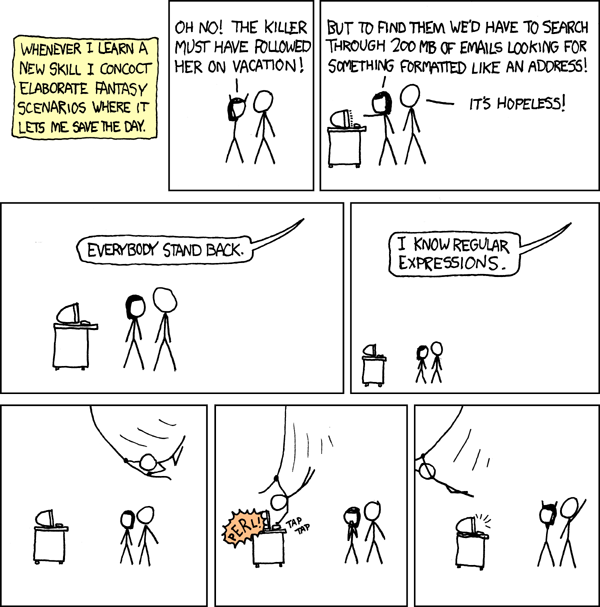
\includegraphics[width=\textwidth]{xkcd_regular_expressions}} 
\smallskip
  
(Komiks autorstwa \href{http://xkcd.com}{Randalla Munroe’a}.)

\chapter{ Programowanie sieciowe. Intensywny kurs}
\label{chap:11}

  
Możliwe, że czytasz ten tekst w oknie przeglądarki internetowej, co oznacza że przynajmniej trochę znasz się na internecie. Rozdział ten zawiera zwięzłe i powierzchowne informacje na temat sposobu działania internetu oraz jak to się ma do języka JavaScript. Głównym tematem jest zatem mówiąc krótko \textbf{programowanie sieciowe} w JavaScript. Trzy kolejne rozdziały zawierają bardziej praktyczną treść, ponieważ pokazuję w nich jak za pomocą JavaScriptu badać i modyfikować strony internetowe.


\begin{center}
• • • • •
\end{center}

  
Internet to mówiąc najprościej sieć komputerów obejmująca większość świata. Dzięki tym sieciom możliwe jest przesyłanie wiadomości między komputerami. Techniczne aspekty działania sieci są bardzo ciekawe, ale niestety temat tej książki jest całkiem inny. Wystarczy pamiętać, że w uproszczeniu jeden komputer, który będziemy nazywać serwerem\index{serwer}, czeka aż inne komputery zaczną się z nim komunikować. Gdy jakiś komputer, klient\index{klient}, nawiąże kontakt z~serwerem, następuje wymiana jakichś danych przy użyciu specjalnego języka zwanego protokołem\index{protokół}.

  
Internet służy do przesyłania wiadomości przy użyciu \emph{wielu} różnych protokołów. Istnieją protokoły do czatowania, udostępniania plików, używane przez szkodliwe programy do kontrolowania komputerów głupków, którzy je zainstalowali itd. Nas interesuje protokół używany przez sieć ogólnoświatową (World Wide Web). Protokół ten nazywa się \textbf{HTTP}\index{HTTP}, co oznacza Hyper Text Transfer Protocol (protokół przesyłania hipertekstu), i służy do pobierania stron internetowych oraz powiązanych z nimi plików.

  
W komunikacji HTTP serwer jest komputerem używanym do przechowywania strony internetowej. Klientem jest komputer, np. Twój, który prosi serwer o przesłanie mu tej strony, aby mógł ją wyświetlić. Taka prośba o~stronę nazywa się \textbf{żądaniem HTTP}\index{żądanie HTTP}.



\begin{center}
• • • • •
\end{center}

  
Strony internetowe i inne pliki dostępne w internecie mają adresy URL\index{URL}, czyli uniwersalne lokalizatory zasobów (ang. Universal Resource Locators). Adres URL wygląda następująco:

  
\begin{verbatim} 
http://acc6.its.brooklyn.cuny.edu/~phalsall/texts/taote-v3.html
 \end{verbatim}
  
Adres URL składa się z trzech części. Pierwsza część, \texttt{http://}, oznacza, że ten adres używa protokołu HTTP. Istnieją jeszcze inne protokoły, np. FTP (ang. File Transfer Protocol — protokół przesyłania plików), które również mogą być używane do tworzenia adresów URL. Druga część, \texttt{acc6.its.brooklyn.cuny.edu}, określa nazwę serwera, na którym znajduje się strona. Na końcu adresu URL, \texttt{/\textasciitilde phalsal/texts/taote-v3.html}, znajduje się nazwa konkretnego pliku na serwerze.

  
Najczęściej z sieci WWW korzysta się przy użyciu przeglądarki internetowej. Gdy użytkownik wpisze adres URL albo kliknie odnośnik, przeglądarka wysyła odpowiednie żądanie HTTP do serwera. Jeśli wszystko się uda, serwer odpowie wysyłając przeglądarce plik, a ta wyświetli go użytkownikowi.

  
Jeśli plikiem tym jest dokument HTML\index{HTML}, zostanie on zaprezentowany jako strona internetowa. Krótki opis języka HTML znajduje się w \hyperref[chap:6]{rozdziale 6}, w którym dowiedzieliśmy się, że w języku tym można odwoływać się do obrazów. W \hyperref[chap:9]{rozdziale 9} dowiedziałeś się też, że strony HTML mogą zawierać elementy \texttt{<script>} ładujące kod JavaScript z plików. Przed wyświetleniem dokumentu HTML przeglądarka pobiera wszystkie dodatkowe zasoby z serwerów, aby dodać je do dokumentu.



\begin{center}
• • • • •
\end{center}

  
Mimo że adres URL powinien wskazywać plik, możliwości serwerów sieciowych są większe niż proste znajdowanie plików i wysyłanie ich do klientów. Serwer może też przetwarzać pliki a nawet możliwe jest, że wybrany plik w ogóle nie istnieje, tylko na serwerze działa specjalny program, który otrzymując żądanie określonego adresu URL generuje na bieżąco odpowiedni dokument.

  
Programy przekształcające i generujące dokumenty na serwerze są wykorzystywane do tworzenia dynamicznych stron internetowych. Plik to po prostu plik i jego zawartość jest zawsze taka sama. Ale jeśli pliki są tworzone na bieżąco dla każdego żądania przez program, to u każdego użytkownika mogą wyglądać inaczej, np. ze względu na to czy użytkownik jest zalogowany lub zdefiniował jakieś ustawienia. Ponadto to bardzo ułatwia zarządzanie treścią stron internetowych — zamiast każdą nową treść wysyłać na serwer w~postaci pliku, dodaje się nowy dokument do jakiegoś centralnego magazynu, a program już wie jak go znaleźć i zaprezentować.

  
Takie rodzaj programowania nazywa się programowaniem serwerowym\index{programowanie serwerowe}. Polega na przetwarzaniu dokumentu przed jego wysłaniem do użytkownika. W większości przypadków dobrze jest też mieć program, który działa \emph{po} wysłaniu strony, gdy użytkownik już ją ogląda. To nazywa się programowaniem po stronie klienta\index{programowanie po stronie klienta}, ponieważ program działa na komputerze klienta. Programowanie po stronie klienta to główne zastosowanie JavaScriptu.



\begin{center}
• • • • •
\end{center}

  
Jednak wykonywanie programów na kliencie ma pewną wadę, której nie da się wyeliminować. Nigdy nie wiadomo, jakie programy będą uruchomione na stronie, którą ma się zamiar odwiedzić. Gdyby program taki mógł wysyłać informacje z naszego komputera, niszczyć pliki albo infiltrować system, to surfowanie po internecie byłoby bardzo niebezpieczne.

  
Dlatego przeglądarki bardzo ograniczają możliwości programów JavaScript. Nie mogą one przeglądać plików użytkownika ani modyfikować niczego, co nie jest związane ze stroną internetową, z którą zostały pobrane. Takie izolowane środowisko programowe nazywa się piaskownicą\index{piaskownica} (ang. sandbox). Nie jest łatwo tak określić uprawnienia programów aby mogły w miarę swobodnie działać, a jednocześnie nie miały możliwości narobienia szkód w komputerze. Co kilka miesięcy jakiś programista JavaScript znajduje kolejne luki w~zabezpieczeniach pozwalające ominąć ograniczenia i wykonywać szkodliwe działania. Twórcy przeglądarek reagują na to modyfikacjami swoich programów tak, aby uniemożliwić wykonywanie odkrytej sztuczki i wszystko wraca do porządku. Dopóki ktoś znowu czegoś nie znajdzie…



\begin{center}
• • • • •
\end{center}

  
Jedną z pierwszych powszechnie znanych sztuczek JavaScript jest użycie metody \texttt{open}\index{window.open}\index{open} obiektu \texttt{window}. Przyjmuje ona jako argument adres URL i~otwiera nowe okno wyświetlając w nim stronę znajdującą się pod tym adresem.

  
\begin{verbatim} 
var perry = window.open("http://www.pbfcomics.com");
 \end{verbatim}
  
Jeśli włączyłeś w \hyperref[chap:6]{rozdziale 6} blokowanie wyskakujących okienek, to najprawdopodobniej okno to zostanie zablokowane. Programy blokujące wyskakujące okienka istnieją nie bez powodu. Programiści sieciowi, z zwłaszcza ci, którzy chcą przyciągnąć uwagę użytkowników do płatnych reklam, nadużywają metody \texttt{window.open} tak bardzo, że większość internautów po prostu jej nienawidzi. Jest ona jednak czasami przydatna i w tej książce również kilka razy zostanie użyta. Ogólna zasada jest taka, że skrypt nie powinien otwierać nowych okien, jeśli użytkownik wyraźnie sobie tego nie zażyczy.

  
Warto zauważyć, że ponieważ metoda \texttt{open} (podobnie jak \texttt{setTimeout} itp.) należy do obiektu \texttt{window}, część \texttt{window.} w jej wywołaniu można opuścić. Gdy funkcja jest wywoływana „normalnie”, to zostaje wywołana jako metoda na obiekcie najwyższego poziomu, którym jest \texttt{window}. Ja jednak uważam, że nazwa \texttt{open} jest trochę za ogólna i wolę pisać \texttt{window.open}, dzięki czemu od razu wiadomo, że chodzi o otwarcie okna.

  
Wartością zwracaną przez metodę \texttt{window.open} jest nowe okno. Jest ono globalnym obiektem dla skryptu działającego w tym oknie i zawiera wszystkie standardowe rzeczy, takie jak konstruktor \texttt{Object} i obiekt \texttt{Math}. Gdy jednak spróbujesz je przejrzeć, większość przeglądarek prawdopodobnie na to nie zezwoli…

  
\begin{verbatim} 
show(perry.Math);
// → Exception: Error: Permission denied to access property 'Math'
\end{verbatim}
  
Jest to związane z działaniem w piaskownicy, o której była mowa wcześniej. Strony otwierane przez naszą przeglądarkę mogą zawierać informacje przeznaczone tylko dla nas, np. w serwisach, w których trzeba się zalogować, i dlatego nie byłoby dobrze gdyby każdy skrypt mógł je odczytać. Wyjątkiem od tej reguły są strony należące do tej samej domeny: jeśli skrypt działający na stronie \texttt{eloquentjavascript.net} otworzy inną stronę w tej samej domenie, to może z nią robić wszystko, co chce.

  
Otwarte okno można zamknąć przy użyciu metody \texttt{close}\index{window.close}\index{close}. Jeśli jeszcze sami go nie zamknęliśmy…

  
\begin{verbatim} 
perry.close();
\end{verbatim}
  
Inne rodzaje poddokumentów, np. ramki (dokumenty w dokumentach), dla programów JavaScript również są oknami i mają własne środowiska JavaScript. W istocie środowisko, do którego masz dostęp w konsoli należy do małej niewidocznej ramki ukrytej gdzieś na tej stronie — dzięki temu trochę trudniej jest przez przypadek popsuć całą stronę podczas zabawy.



\begin{center}
• • • • •
\end{center}

  
Każdy obiekt okna ma własność \texttt{document}\index{document} zawierającą obiekt reprezentujący dokument wyświetlony w tym oknie. Obiekt ten zawiera np. własność \texttt{location}\index{document.location} zawierającą informacje o adresie URL dokumentu.

  
\begin{verbatim} 
show(document.location.href);
// → "http://www.bt4.pl/kursy/javascript/wszystko-jasne/
//    r11-programowanie-sieciowe/"
\end{verbatim}
  
Ustawiając własność \texttt{document.location.href} na inny adres URL można spowodować wczytanie przez przeglądarkę innego dokumentu. Obiekt \texttt{document} zawiera także metodę \texttt{write}\index{document.write}. Służy ona do wstawiania do dokumentu kodu HTML, który trzeba jej przekazać w postaci łańcucha. Gdy zostanie zastosowana do w pełni załadowanego dokumentu, to zastąpi go w całości otrzymanym kodem HTML, czego zazwyczaj nie chcemy. Najczęściej skrypt wywołuje ją w czasie ładowania dokumentu i wówczas kod HTML zostaje wstawiony do dokumentu w miejscu elementu \texttt{script} odpowiedzialnego za jej dodanie. Jest to prosty sposób na dodanie dynamicznych elementów do strony. Na przykład poniżej znajduje się banalnie prosty dokument pokazujący bieżącą godzinę.

  
\begin{verbatim} 
print(timeWriter);
var time = viewHTML(timeWriter);
 \end{verbatim}
  
\begin{verbatim} 
time.close();
 \end{verbatim}
  
W \hyperref[chap:12]{rozdziale 12} znajduje się opis bardziej klarownych i wszechstronnych sposobów modyfikowania dokumentów, ale czasami metoda \texttt{document.write} jest najprostszym i najlepszym rozwiązaniem.



\begin{center}
• • • • •
\end{center}

  
Kolejną dziedziną dotyczącą stron internetowych, w której język JavaScript często znajduje zastosowanie są formularze\index{formularz}. Kilka słów wyjaśnienia dla tych, którzy nie wiedzą do czego służą formularze.

  
Najprostsze żądanie HTTP to zwykła prośba do serwera o przesłanie pliku. Gdy żądany plik nie jest pasywnym plikiem lecz plikiem zwracanym przez program działający na serwerze, to czasami do żądania warto dołączyć także inne informacje niż tylko adres URL. Dlatego żądania HTTP mogą zawierać dodatkowe parametry. Oto przykład:

  
\begin{verbatim} 
http://www.google.com/search?q=aztec%20empire
\end{verbatim}
  
Po nazwie pliku (\texttt{/search}) znajduje się znak zapytania, po którym z kolei znajdują się parametry. To żądanie zawiera jeden parametr o nazwie \texttt{q} (prawdopodobnie od słowa ang. „query” czyli „zapytanie”), którego wartość to \texttt{aztec empire}. Ciąg \texttt{\%20} oznacza spację. W wartościach tych nie mogą występować niektóre znaki, np. spacje, ampersand (\&) i znaki zapytania. Są one zastępowane specjalnymi kodami składającymi się ze znaku \texttt{\%} i wartości liczbowej\footnote{Wartości kodów znakowych są określone w standardzie ASCII, w którym każdej literze alfabetu łacińskiego i symbolowi przypisana jest liczba z przedziału 0-127. Standard ten jest prekursorem standardou Unicode, o którym była mowa w \hyperref[chap:2]{rozdziale 2}.}. Znak procent w tym przypadku pełni taką samą rolę, jak ukośnik wsteczny w wyrażeniach regularnych, tylko trochę lepiej wygląda.

  
W języku JavaScript dostępne są funkcje \texttt{encodeURIComponent}\index{encodeURIComponent} i \texttt{decodeURIComponent}\index{decodeURIComponent} służące do dodawania tych kodów do łańcuchów i usuwania ich.

  
\begin{verbatim} 
var encoded = encodeURIComponent("aztec empire");
show(encoded);
// → "aztec%20empire"
show(decodeURIComponent(encoded));
// → "aztec empire"
\end{verbatim}
  
Gdy żądanie zawiera więcej parametrów, rozdziela się je znakami ampersand:

  
\begin{verbatim} 
http://www.google.com/search?q=aztec%20empire&lang=pl
\end{verbatim}


\begin{center}
• • • • •
\end{center}

  
Formularz mówiąc najprościej to narzędzie ułatwiające użytkownikom przeglądarek tworzenie takich parametryzowanych adresów URL. W formularzu znajdują się pola, np. tekstowe i wyboru, które można zaznaczać oraz obiekty pozwalające wybrać jedna z kilku wartości itp. Najczęściej dostępny jest też przycisk zatwierdzania formularza oraz niewidoczny dla użytkownika adres URL wskazujący program, który ma być użyty do przetworzenia danych z tego formularza. Kliknięcie przycisku zatwierdzania lub naciśnięcie klawisza Enter powoduje dodanie informacji wprowadzonych w formularzu do adresu URL jako parametrów i wysłanie żądania pod taki adres.

  
Poniżej znajduje się kod HTML prostego formularza:

  
\begin{verbatim} 
<form name="userinfo" method="get" action="info.html">
  <p>Podaj nam swoje dane, abyśmy mogli Ci wysyłać
  spam.</p>
  <p>Imię i nazwisko: <input type="text" name="name"/></p>
  <p>E-Mail: <input type="text" name="email"/></p>
  <p>Płeć: <select name="sex">
            <option>Mężczyzna</option>
            <option>Kobieta</option>
            <option>Inna</option>
          </select></p>
  <p><input name="send" type="submit" value="Wyślij!"/></p>
</form>
 \end{verbatim}
  
Posługując się nazwą formularza można uzyskać dostęp do niego z poziomu JavaScriptu, co za chwilę zostanie pokazane. Nazwy pól determinują nazwy parametrów HTTP używanych do przechowywania ich wartości. Zatwierdzenie tego formularza może spowodować utworzenie następującego adresu URL:

  
\begin{verbatim} 
http://planetspam.com/info.html?name=Tadek&email=tadek@zork.com&sex=Mężczyzna
\end{verbatim}
  
Formularze mają jeszcze wiele innych elementów i własności, ale my skoncentrujemy się tylko na tych kilku podstawowych, ponieważ przede wszystkim interesuje nas JavaScript.



\begin{center}
• • • • •
\end{center}

  
Atrybut \texttt{method="get"} w przedstawionym formularzu oznacza, że dane wpisane w polach tego formularza mają zostać zakodowane w postaci parametrów adresu URL. Istnieje też inna metoda wysyłania parametrów o~nazwie \texttt{post}. Żądanie HTTP wysłane metodą \texttt{post} oprócz adresu URL zawiera dodatkowo blok danych. Formularz wysyłany metodą \texttt{post} wstawia wartości swoich parametrów do tego bloku zamiast do adresu URL.

  
Metoda \texttt{post} lepiej nadaje się do przesyłania w formularzach dużych ilości danych, ponieważ wysyłanie ich metodą \texttt{get} spowodowałoby powstanie kilometrowych adresów URL. Jednak różnica między tymi dwiema metodami to nie tylko kwestia urody adresów. Metody \texttt{get} zwyczajowo używa się do wysyłania do serwera żądań dokumentów, natomiast \texttt{post} do wysyłania żądań wykonania czegoś na serwerze, co spowoduje tam jakąś zmianę. Na przykład żądanie listy ostatnio opublikowanych na forum internetowym wpisów wysłano by metodą \texttt{get}, natomiast żądanie dodania nowego wpisu — metodą \texttt{post}. Trzymanie się tej zasady ma uzasadnienie — automaty przeglądające sieć, np. wyszukiwarki internetowe, zazwyczaj wykonują tylko żądania \texttt{get}. Gdyby za pomocą żądań \texttt{get} dokonywano zmian na stronach,  te nieszkodliwe z założenia narzędzia mogłyby narobić wiele szkód.



\begin{center}
• • • • •
\end{center}

  
Gdy przeglądarka wyświetla stronę zawierającą formularz, programy JavaScript mogą przeglądać i modyfikować wartości wprowadzane w polach tego formularza. To umożliwia wykonywanie różnych sztuczek, takich jak sprawdzanie wartości przed wysłaniem ich na serwer czy automatyczne wypełnianie niektórych pól.

  
Powyższy formularz znajduje się w pliku \texttt{example\_getinfo.html}. Otwórz go.

  
\begin{verbatim} 
var form = window.open("/wp-content/ejs/example_getinfo.html");
\end{verbatim}
  
Gdy adres URL nie zawiera nazwy serwera, to nazywa się adresem względnym\index{adres względny}. Adresy względne są przez przeglądarki interpretowane jako odnoszące się do plików znajdujących się na tym samym serwerze, co bieżący dokument. Jeśli nie zaczynają się od ukośnika, brana jest ścieżka (lub katalog) bieżącego dokumentu i do tego dodaje się podaną ścieżkę.

  
Dodamy do naszego formularza mechanizm sprawdzający poprawność jego wypełnienia, który pozwoli na jego zatwierdzenie tylko, gdy pole nazwiska nie będzie puste, a pole adresu e-mail będzie wyglądać na poprawnie wypełnione. Jako że nie chcemy już aby formularz był wysyłany natychmiast po naciśnięciu przycisku Wyślij!, zmienimy jego atrybut \texttt{type} z \texttt{submit} na \texttt{button}, dzięki czemu stanie się zwykłym przyciskiem. ― W \hyperref[chap:13]{rozdziale 13} opisana jest \emph{o wiele} lepsza metoda zrobienia tego, ale tutaj wystarczy nam takie uproszczone rozwiązanie.



\begin{center}
• • • • •
\end{center}

  
\index{attach}Aby móc pracować z nowo otwartym oknem (jeśli je zamknąłeś, to otwórz je znowu), musimy powiązać je z konsolą:

  
\begin{verbatim} 
attach(form);
// → Powiązanie z oknem „Zarejestruj konto w Planet Junkmail”.
\end{verbatim}
  
Gdy to zrobisz, kod w konsoli będzie uruchamiany w określonym oknie. Aby sprawdzić czy rzeczywiście działamy w tym oknie, co trzeba, możemy zajrzeć do własności \texttt{location} i \texttt{title} dokumentu.

  
\begin{verbatim} 
print(document.location.href);
// → http://www.bt4.pl/wp-content/ejs/example_getinfo.html
print(document.title);
// → Zarejestruj konto w Planet Junkmail
\end{verbatim}
  
Ponieważ otworzyliśmy nowe środowisko, wcześniej zdefiniowane zmienne, jak np. \texttt{form}, nie są już dostępne.

  
\begin{verbatim} 
show(form);
\end{verbatim}
  
\index{detach}Aby wrócić do początkowego środowiska, możemy posłużyć się funkcją \texttt{detach} (bez argumentów). Ale wcześniej musimy dodać system sprawdzający do formularza.



\begin{center}
• • • • •
\end{center}

  
Z każdym elementem HTML znajdującym się w dokumencie jest powiązany obiekt JavaScript. Obiektów tych można używać do przeglądania i manipulowania prawie wszystkimi aspektami dokumentu. W tym rozdziale będziemy używać obiektów formularzy i pól formularzy w podstawowy sposób, a w \hyperref[chap:12]{rozdziale 12} zajmiemy się nimi bardziej szczegółowo.

  
\index{document.forms}Obiekt \texttt{document} ma własność o nazwie \texttt{forms} zawierający łącza do wszystkich formularzy znajdujących się w dokumencie, wg nazw. Nasz formularz ma atrybut \texttt{name="userinfo"}, a więc można go znaleźć we własności o nazwie \texttt{userinfo}.

  
\begin{verbatim} 
var userForm = document.forms.userinfo;
print(userForm.method);
// → get
print(userForm.action);
// → http://www.bt4.pl/wp-content/ejs/example_getinfo.html
\end{verbatim}
  
W tym przypadku atrybuty \texttt{method} i \texttt{action}, które zostały przekazane do elementu HTML \texttt{form} również są dostępne jako własności obiektu JavaScript. Najczęściej tak jest, ale nie zawsze: niektóre atrybuty HTML w~JavaScript mają inne nazwy, a niektórych nie ma w ogóle. Sposób dostania się do wszystkich własności przedstawiłem w \hyperref[chap:12]{rozdziale 12}.

  
Obiekt elementu \texttt{form} ma własność \texttt{elements} odnoszącą się do obiektu zawierającego wszystkie pola formularza wg nazw.

  
\begin{verbatim} 
var nameField = userForm.elements.name;
nameField.value = "Kowalski";
\end{verbatim}
  
Obiekty pól tekstowych mają własność \texttt{value}, przy użyciu której można odczytywać i zmieniać ich zawartość. Jeśli wykonasz powyższy kod, zauważysz, że w polu nazwiska formularza pojawi się nazwisko.



\begin{center}
• • • • •
\end{center}

  
\section*{Ćwiczenie 11.1}
\label{sec:11.1}
  
    
Dzięki możliwości odczytywania wartości pól formularza możemy napisać funkcję \texttt{validInfo}, która pobiera jako argument obiekt formularza i zwraca wartość logiczną: \texttt{true} jeśli pole \texttt{name} nie jest puste, a pole \texttt{email} zawiera coś, co wygląda jak adres e-mail oraz \texttt{false} w pozostałych przypadkach. Poniżej znajduje się kod implementacji tej funkcji.

  
[\hyperref[sol:11.1]{pokaż rozwiązanie}]
  


\begin{center}
• • • • •
\end{center}

  
Pozostało nam już tylko określenie czynności, jaka ma zostać wykonana, gdy ktoś kliknie przycisk ,,Wyślij!''. Na razie jego kliknięcie nic nie zmienia. Ale można to zmienić korzystając z własności \texttt{onclick}.

  
\begin{verbatim} 
userForm.elements.send.onclick = function() {
  alert("Klik.");
};
\end{verbatim}
  
Podobnie jak w przypadku akcji przekazywanych do funkcji \texttt{setInterval} i \texttt{setTimeout} (\hyperref[chap:8]{rozdział 8}), wartość zapisywana w \texttt{onclick}\index{onclick} (lub podobnej) własności może być funkcją lub łańcuchem kodu JavaScript. Tym razem przekazaliśmy funkcję otwierającą okienko alertu. Kliknij przycisk.



\begin{center}
• • • • •
\end{center}

  
\section*{Ćwiczenie 11.2}
\label{sec:11.2}
  
    
Na zakończenie prac nad systemem weryfikacji własności \texttt{onclick} przycisku nadamy nową wartość ― funkcję sprawdzającą formularz i zatwierdzającą go, gdy jest poprawnie wypełniony oraz wyświetlającą ostrzeżenie, gdy zawiera błędy. Przyda się wiedza, że obiekty formularzy mają metodę \texttt{submit}\index{submit}, która nie przyjmuje żadnych argumentów i tylko zatwierdza formularz.

  
[\hyperref[sol:11.2]{pokaż rozwiązanie}]


\begin{center}
• • • • •
\end{center}

  
Inna sztuczka związana z polami wejściowymi formularzy i innymi elementami, które można wybierać, np. przyciskami i łączami, jest związana z metodą \texttt{focus}\index{focus}. Jeśli ma się pewność, że po wejściu na stronę użytkownik zacznie wprowadzanie danych od konkretnego pola, można automatycznie umieścić w nim kursor, aby użytkownik nie musiał w nim klikać ani przechodzić do niego w żaden inny sposób.

  
\begin{verbatim} 
userForm.elements.name.focus();
\end{verbatim}
  
Ponieważ formularz znajduje się w innym oknie, w niektórych przeglądarkach może nie być oczywiste, że coś zostało wybrane. Niektóre strony automatycznie przenoszą kursor do następnego pola, gdy poprzednie wydaje się wypełnione, np. gdy użytkownik wpisze kod pocztowy. Nie należy z tym przesadzać, ponieważ taka funkcja sprawia, że formularz zachowuje się w nieoczekiwany sposób. Jeśli użytkownik jest przyzwyczajony do zmieniania pól formularza za pomocą klawisza Tab albo źle coś wpisze i zechce to poprawić, to takie magiczne przeskakiwanie kursora może go bardzo denerwować.



\begin{center}
• • • • •
\end{center}

  
\begin{verbatim} 
detach();
// → Usuwanie powiązania z oknem „Zarejestruj konto w Planet Junkmail”.
\end{verbatim}
  
Przetestuj weryfikatora. Gdy wpiszesz prawidłowe dane i klikniesz przycisk, formularz powinien zostać zatwierdzony. Jeśli w tym czasie konsola będzie cały czas do niego podłączona, to się odłączy, ponieważ nastąpi ponowne wczytanie strony i utworzenie nowego środowiska JavaScript.

  
Jeśli jeszcze nie zamknąłeś okna formularza, to spowoduje jego zamknięcie.

  
\begin{verbatim} 
form.close();
\end{verbatim}


\begin{center}
• • • • •
\end{center}

  
Opisane powyżej czynności mogą się wydawać proste, ale uwierz mi, programowania po stronie klienta to nie jest bułka z masłem. Czasami bywa niesamowicie trudne. Dlaczego? Ponieważ programy przeznaczone do działania w komputerze klienta muszą prawidłowo działać we wszystkich popularnych przeglądarkach. A każda z ich działa trochę inaczej. Co gorsza każda taka aplikacja ma własny zbiór usterek. Niech Ci się nie wydaje, że skoro program jest własnością firmy dysponującej milionowym budżetem, to na pewno nie zawiera błędów. Dlatego my, programiści, musimy skrupulatnie testować nasze programy, znajdować błędy i opracowywać poprawne rozwiązania.

  
Możesz sobie pomyśleć: „Po prostu zgłoszę wszelkie usterki\index{błąd}, jakie znajdę do producenta przeglądarki, aby szybko je usunął i wszystko będzie w~porządku”. Niestety czeka Cię wielkie rozczarowanie. Producenci często nie spieszą się z poprawianiem błędów, a do perfekcji umiejętność tę opanował Microsoft ze swoją przeglądarką Internet Explorer, chociaż w jej najnowszych wersjach sytuacja uległa już znacznej poprawie. Błędy są i będą.

  
Ale nie zrażaj się. Jeśli masz obsesję na punkcie znajdowania nowych wyzwań, to tutaj na pewno znajdziesz ich wiele. A jeśli nie lubisz marnować czasu, to wystarczy, że będziesz unikać słabiej poznanych zakamarków funkcjonowania przeglądarek, aby nie wpaść w poważne kłopoty.

\chapter{ Obiektowy model dokumentu}
\label{chap:12}

  
W \hyperref[chap:11]{rozdziale 11} używaliśmy obiektów JavaScript odnoszących się do elementów \texttt{form} i \texttt{input} dokumentu HTML. Obiekty te należą do struktury o nazwie \textbf{DOM}\index{DOM} (ang. Document-Object Model — obiektowy model dokumentu)\index{obiektowy model dokumentu}. W~modelu tym reprezentację ma każdy element znajdujący się w dokumencie. Można go tam znaleźć i coś z nim zrobić.

  
Dokumenty HTML mają strukturę hierarchiczną. Każdy element (lub znacznik) z wyjątkiem głównego elementu \texttt{<html>} znajduje się w innym elemencie, który jest jego rodzicem. Element mający rodzica również może zawierać elementy potomne. Można to sobie wyobrazić, jako drzewo rodzinne.

\bigskip 
\centerline{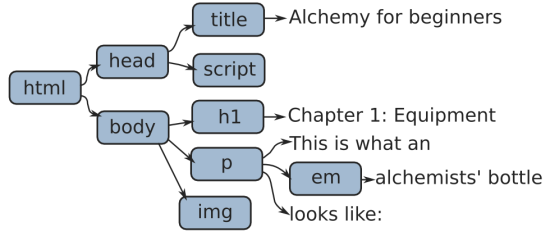
\includegraphics[width=\textwidth]{html}} 
\smallskip
  
Obiektowy model dokumentu opiera się właśnie na takiej reprezentacji dokumentu. Zwróć uwagę, że przedstawione drzewo zawiera dwa rodzaje elementów: węzły reprezentowane przez niebieskie pola i fragmenty zwykłego tekstu. Wkrótce się dowiesz, że urywki tekstu zachowują się trochę inaczej niż inne elementy. Na przykład nie mogą mieć dzieci.

  
Otwórz plik \texttt{example\_alchemy.html} zawierający dokument przedstawiony na  rysunku i powiąż go z konsolą.

  
\begin{verbatim} 
attach(window.open("/wp-content/ejs/example_alchemy.html"));
 \end{verbatim}
  
\index{document.documentElement}Dostęp do obiektu stanowiącego korzeń drzewa dokumentu, węzła \texttt{html}, można uzyskać poprzez własność \texttt{documentElement} obiektu \texttt{document}. Najczęściej jednak potrzebny jest dostęp do części \texttt{body} dokumentu dostępnej jako \texttt{document.body}\index{document.body}.



\begin{center}
• • • • •
\end{center}

  
Łącza między tymi węzłami są dostępne jako własności obiektów węzłów. Każdy obiekt DOM ma własność \texttt{parentNode}\index{parentNode}, która odnosi się do obiektu, w~którym ten obiekt się znajduje (jeżeli w ogóle ma rodzica). Ci rodzice również mają łącza wskazujące na ich dzieci, ale ponieważ dzieci może być wiele, są one przechowywane w pseudotablicy o nazwie \texttt{childNodes}\index{childNodes}.

  
\begin{verbatim} 
show(document.body);
show(document.body.parentNode);
show(document.body.childNodes.length);
 \end{verbatim}
  
Dla wygody dostępne są też łącza o nazwach \texttt{firstChild}\index{firstChild} i \texttt{lastChild}\index{lastChild} wskazujące pierwszy i ostatni element dziecko w węźle lub \texttt{null} jeśli element nie zawiera żadnego elementu.

  
\begin{verbatim} 
show(document.documentElement.firstChild);
show(document.documentElement.lastChild);
 \end{verbatim}
  
Ostatnie dwie własności to \texttt{nextSibling}\index{nextSibling} i \texttt{previousSibling}\index{previousSibling} wskazujące węzły znajdujące się „obok” określonego węzła ― są to węzły mające tego samego rodzica i znajdujące się przed lub za określonym elementem. Jeśli nie ma takiego elementu, własności zawierają wartość \texttt{null}.

  
\begin{verbatim} 
show(document.body.previousSibling);
show(document.body.nextSibling);
 \end{verbatim}


\begin{center}
• • • • •
\end{center}

  
Aby dowiedzieć się, czy wybrany węzeł reprezentuje tylko tekst czy węzeł HTML, można sprawdzić jego własność \texttt{nodeType}\index{nodeType}. Wartość \texttt{1} oznacza zwykły węzeł, a \texttt{3} węzeł tekstowy. Istnieją też inne rodzaje obiektów mające własność \texttt{nodeType}, np. obiekt \texttt{document}, którego wartość to \texttt{9}, ale najczęściej używa się jej do odróżniania węzłów tekstowych od innych.

  
\begin{verbatim} 
function isTextNode(node) {
  return node.nodeType == 3;
}

show(isTextNode(document.body));
show(isTextNode(document.body.firstChild.firstChild));
 \end{verbatim}
  
Zwykłe węzły mają własność o nazwie \texttt{nodeName}\index{nodeName} określającą typ reprezentowanego przez nie elementu HTML. Natomiast węzły tekstowe mają własność \texttt{nodeValue}\index{nodeValue} zawierającą ich treść.

  
\begin{verbatim} 
show(document.body.firstChild.nodeName);
show(document.body.firstChild.firstChild.nodeValue);
 \end{verbatim}
  
Nazwy węzłów są zawsze pisane wielkimi literami i trzeba to brać pod uwagę w wyrażeniach porównawczych.

  
\begin{verbatim} 
function isImage(node) {
  return !isTextNode(node) && node.nodeName == "IMG";
}

show(isImage(document.body.lastChild));
 \end{verbatim}


\begin{center}
• • • • •
\end{center}

  
\section*{Ćwiczenie 12.1}
\label{sec:12.1}
  
    
Napisz funkcję o nazwie \texttt{asHTML} pobierającą węzeł DOM i zwracającą łańcuch reprezentujący tekst HTML tego węzła i jego dzieci. Możesz zignorować atrybuty, tzn. wystarczy wyświetlić węzły w formie \texttt{<nazwawezla>}. Możesz używać funkcji \texttt{escapeHTML} z \hyperref[chap:10]{rozdziału 10}, aby odpowiednio dostosować treść węzłów tekstowych.

    
Podpowiedź: Rekurencja!

  
[\hyperref[sol:12.1]{pokaż rozwiązanie}]


\begin{center}
• • • • •
\end{center}

  
W istocie węzły mają coś podobnego do funkcji \texttt{asHTML}. Przy użyciu własności \texttt{innerHTML}\index{innerHTML} można pobierać tekst HTML \emph{z wnętrza} węzła, bez znaczników samego węzła. Dodatkowo niektóre przeglądarki udostępniają też własność \texttt{outerHTML}, która zawiera również sam węzeł.

  
\begin{verbatim} 
print(document.body.innerHTML);
\end{verbatim}
  
Niektóre z tych własności można też modyfikować. Zmiana własności \texttt{innerHTML} zwykłego węzła albo \texttt{nodeValue} węzła tekstowego spowoduje zmianę ich treści. Należy podkreślić, że w pierwszym przypadku podany łańcuch jest interpretowany jako HTML, podczas gdy w drugim — jako zwykły tekst.

  
\begin{verbatim} 
document.body.firstChild.firstChild.nodeValue =
  "Rozdział 1: Głęboka prawda ukryta w butelce";
\end{verbatim}
  
Albo…

  
\begin{verbatim} 
document.body.firstChild.innerHTML =
  "Znasz już element blink? <blink>Cudowny!</blink>";
\end{verbatim}


\begin{center}
• • • • •
\end{center}

  
Do tej pory dostęp do węzłów uzyskiwaliśmy przemierzając szeregi własności \texttt{firstChild} i \texttt{lastChild}. Tak też można, ale wymaga to dużo pisania i łatwo spowodować błąd. Jeśli na początku dokumentu wprowadzimy nowy węzeł, to \texttt{document.body.firstChild} nie będzie już odwoływać się do elementu \texttt{h1} i kod, w którym przyjęto takie założenie przestanie poprawnie działać. Co więcej, niektóre przeglądarki dodają węzły tekstowe dla spacji i znaków nowego wiersza znajdujących się między elementami, a inne tego nie robią. Przez to \textbf{drzewo DOM} w każdej przeglądarce może być trochę inne.

  
Alternatywnym rozwiązaniem jest przypisanie każdemu elementowi, do którego chce się uzyskać dostęp atrybutu \texttt{id}. Na przykładowej stronie obraz ma identyfikator \texttt{picture}, przy użyciu którego możemy znaleźć ten element.

  
\begin{verbatim} 
var picture = document.getElementById("picture");
show(picture.src);
picture.src = "/wp-content/uploads/ostrich.png";
\end{verbatim}
  
\index{document.getElementById}Wpisując nazwę \texttt{getElementById} nie wpisz przez pomyłkę na końcu wielkiej litery. Ponadto, jeśli musisz ją często wpisywać, grozi Ci zespół cieśni kanału nadgarstka. Ponieważ nazwa \texttt{document.getElementById} jest o wiele za długa, jak na bardzo często używaną operację, programiści JavaScript maksymalnie ją skrócili do postaci \texttt{\$}\index{\$}. Jak wiadomo znak \texttt{\$} jest w języku JavaScript literą, a więc może być używany jako nazwa zmiennej.

  
\begin{verbatim} 
function $(id) {
  return document.getElementById(id);
}
show($("picture"));
\end{verbatim}
  
Węzły DOM mają też metodę \texttt{getElementsByTagName}\index{getElementsByTagName} (kolejna fajna, krótka nazwa), która pobiera nazwę elementu i zwraca wszystkie węzły tego typu, jakie znajdują się w węźle, na rzecz którego została wywołana.

  
\begin{verbatim} 
show(document.body.getElementsByTagName("BLINK")[0]);
\end{verbatim}


\begin{center}
• • • • •
\end{center}

  
Kolejną czynnością, jaką można wykonywać na drzewie DOM jest tworzenie nowych węzłów. Dzięki temu można w dowolnym momencie dodawać elementy do dokumentu, co pozwala uzyskać różne ciekawe efekty. Niestety interfejs jest niesamowicie niezgrabny. Można go jednak trochę poprawić używając paru funkcji pomocniczych.

  
Obiekt \texttt{document} ma metody \texttt{createElement}\index{document.createElement} i \texttt{createTextNode}\index{document.createTextNode}. Pierwsza służy do tworzenia zwykłych węzłów, a druga zgodnie z nazwą do tworzenia węzłów tekstowych.

  
\begin{verbatim} 
var secondHeader = document.createElement("H1");
var secondTitle = document.createTextNode("Rozdział 2: Poważna magia");
\end{verbatim}
  
Następnie wstawimy tytuł do elementu \texttt{h1} i dodamy element do dokumentu. Najprostszym sposobem na zrobienie tego jest użycie metody \texttt{appendChild}\index{appendChild}, którą można wywołać na każdym nietekstowym węźle.

  
\begin{verbatim} 
secondHeader.appendChild(secondTitle);
document.body.appendChild(secondHeader);
\end{verbatim}
  
Nowym węzłom często przypisuje się jakieś atrybuty. Na przykład element \texttt{img} (obraz) jest bezużyteczny, jeśli nie ma atrybutu \texttt{src} wskazującego grafikę, która ma zostać wyświetlona. Większość atrybutów można traktować jako własności węzłów DOM, ale istnieją też metody \texttt{setAttribute}\index{setAttribute} i~\texttt{getAttribute}\index{getAttribute}, które umożliwiają dostęp do atrybutów w bardziej ogólny sposób:

  
\begin{verbatim} 
var newImage = document.createElement("IMG");
newImage.setAttribute("src", "/wp-content/uploads/Hiva-Oa.png");
document.body.appendChild(newImage);
show(newImage.getAttribute("src"));
\end{verbatim}


\begin{center}
• • • • •
\end{center}

  
Jednak gdy trzeba utworzyć większą liczbę węzłów, wielokrotne wywoływanie metody \texttt{document.createElement} lub \texttt{document.createTextNode}, a~następnie dodawanie atrybutów i węzłów potomnych po jednym na raz jest bardzo żmudne. Na szczęście napisanie funkcji, która wszystko za nas zrobi nie jest trudne. Zanim to zrobimy, musimy zająć się jeszcze jednym drobiazgiem ― metoda \texttt{setAttribute} poprawnie działa w większości przeglądarek internetowych, ale w Internet Explorerze może sprawiać problemy. Nazwy niektórych atrybutów HTML mają w języku JavaScript specjalne znaczenie, przez co odpowiadające im nazwy własności obiektów są nieco zmodyfikowane. Atrybut \texttt{class} ma nazwę \texttt{className}\index{className}, \texttt{for} — \texttt{htmlFor}, a~\texttt{checked} — \texttt{defaultChecked}. W Internet Explorerze metody \texttt{setAttribute} i~\texttt{getAttribute} również działają z tymi zmienionymi nazwami, zamiast używać oryginalnych nazw z HTML-a, co może być mylące. Ponadto w przeglądarce tej atrybutu \texttt{style}\index{style}, który razem z atrybutem \texttt{class} zostanie opisany w dalszej części tego rozdziału, nie można ustawiać przy użyciu metody \texttt{setAttribute}.

  
Obejście tego może wyglądać tak:

  
\begin{verbatim} 
function setNodeAttribute(node, attribute, value) {
  if (attribute == "class")
    node.className = value;
  else if (attribute == "checked")
    node.defaultChecked = value;
  else if (attribute == "for")
    node.htmlFor = value;
  else if (attribute == "style")
    node.style.cssText = value;
  else
    node.setAttribute(attribute, value);
}
\end{verbatim}
  
W każdym przypadku, w którym Internet Explorer odbiega od reszty przeglądarek robimy coś, co działa we wszystkich przypadkach. Nie przejmuj się szczegółami — jest to brzydka sztuczka, której wolelibyśmy nie stosować, ale zmuszają nas do tego niepokorne przeglądarki. Teraz możemy napisać prostą funkcję do tworzenia elementów DOM.

  
\begin{verbatim} 
function dom(name, attributes) {
  var node = document.createElement(name);
  if (attributes) {
    forEachIn(attributes, function(name, value) {

      setNodeAttribute(node, name, value);
    });
  }
  for (var i = 2; i < arguments.length; i++) {
    var child = arguments[i];
    if (typeof child == "string")
      child = document.createTextNode(child);
    node.appendChild(child);
  }
  return node;
}

var newParagraph = 
  dom("P", null, "Akapit zawierający ",
      dom("A", {href: "http://en.wikipedia.org/wiki/Alchemy"},
          "łącze"),
      " wewnątrz.");
document.body.appendChild(newParagraph);
\end{verbatim}
  
Funkcja \texttt{dom}\index{dom} tworzy węzeł DOM. Jej pierwszy argument określa nazwę elementu reprezentowanego przez tworzony węzeł, a drugi argument jest obiektem zawierającym atrybuty tego węzła lub wartość \texttt{null}, jeśli nie ma atrybutów. Dalej może znajdować się dowolna liczba argumentów, które zostaną dodane do węzła jako dzieci. Jeśli wśród nich znajdą się łańcuchy, to zostaną najpierw umieszczone w węźle tekstowym.



\begin{center}
• • • • •
\end{center}

  
Metoda \texttt{appendChild} nie jest jedynym sposobem na wstawianie węzłów do innych węzłów. Jeśli nowy węzeł nie może znajdować się na końcu swojego rodzica, można użyć metody \texttt{insertBefore}\index{insertBefore}, aby dodać węzeł przed innym węzłem dzieckiem. Nowy węzeł podaje się jako pierwszy argument, a istniejący — jako drugi.

  
\begin{verbatim} 
var link = newParagraph.childNodes[1];
newParagraph.insertBefore(dom("STRONG", null, "great "), link);
 \end{verbatim}
  
Jeśli wstawi się gdzieś węzeł mający już rodzica (\texttt{parentNode}), węzeł ten automatycznie zostanie usunięty z dotychczasowego miejsca ― żaden węzeł nie może występować w drzewie dokumentu więcej niż raz.

  
Gdy trzeba zastąpić węzeł innym, należy użyć metody \texttt{replaceChild}\index{replaceChild}, która jako pierwszy argument przyjmuje nowy węzeł, a jako drugi — stary.

  
\begin{verbatim} 
newParagraph.replaceChild(document.createTextNode("luźne "),
                          newParagraph.childNodes[1]);
\end{verbatim}
  
W końcu za pomocą metody \texttt{removeChild}\index{removeChild} usuwa się węzły potomne. Zwróć uwagę, że wywołuje się ją na \emph{rodzicu} węzła, który ma zostać usunięty i przekazuje się jej element potomny jako argument.

  
\begin{verbatim} 
newParagraph.removeChild(newParagraph.childNodes[1]);
\end{verbatim}


\begin{center}
• • • • •
\end{center}

  
\section*{Ćwiczenie 12.2}
\label{sec:12.2}
  
    
Napisz wygodną funkcję \texttt{removeElement}\index{removeElement} usuwającą przekazany jej w argumencie węzeł DOM z węzła nadrzędnego.

  
[\hyperref[sol:12.2]{pokaż rozwiązanie}]


\begin{center}
• • • • •
\end{center}

  
Podczas tworzenia nowych węzłów i przenoszenia istniejących należy pamiętać o następującej zasadzie: węzłów nie można wstawiać do dokumentu innego niż ten, w którym zostały utworzone. Oznacza to, że jeśli są dodatkowe ramki lub otwarte okna, nie można pobrać części dokumentu z jednego z tych obiektów i przenieść go do innego oraz węzły utworzone przy użyciu metod jednego obiektu \texttt{document} muszą pozostać w tym dokumencie. Niektóre przeglądarki, a konkretnie Firefox, nie przestrzegają tej zasady, przez co kod ją łamiący w Firefoksie zadziała.


\begin{center}
• • • • •
\end{center}

  
Przykładem użycia funkcji \texttt{dom} w jakimś pożytecznym celu jest program pobierający obiekty JavaScript i tworzący z nich tabelę\index{tabela}. W języku HTML tabele tworzy się przy użyciu elementów, których nazwy zaczynają się od litery „t”, np.:

  
\begin{verbatim} 
<table>
  <tbody>
    <tr> <th>Drzewo</th> <th>Kwiaty  </th> </tr>
    <tr> <td>Jabłoń</td> <td>Białe   </td> </tr>
    <tr> <td>Koral </td> <td>Czerwone</td> </tr>
    <tr> <td>Sosna </td> <td>Brak    </td> </tr>
  </tbody>
</table>
\end{verbatim}
  
Elementy \texttt{tr} reprezentują wiersze tabeli. Elementy \texttt{th} i \texttt{td} to komórki, przy czym \texttt{td} to zwykłe komórki, a \texttt{th} to komórki nagłówka, których zawartość lekko się wyróżnia. Element \texttt{tbody} (ang. table body — treść tabeli) nie jest wymagany w samym języku HTML, ale musi być użyty, gdy tabelę tworzy się z węzłów DOM, ponieważ Internet Explorer nie wyświetla tabel utworzonych bez tego elementu.


\begin{center}
• • • • •
\end{center}

  
\section*{Ćwiczenie 12.3}
\label{sec:12.3}
  
    
Funkcja \texttt{makeTable} przyjmuje jako argumenty dwie tablice. Pierwsza zawiera obiekty JavaScript, które mają być wstawione do tabeli, a druga — łańcuchy określające nazwy kolumn tej tabeli i własności obiektów, które mają zostać pokazane w tych kolumnach. Na przykład poniższe wywołanie tworzy wcześniej pokazaną tabelę:

    
\begin{verbatim} 
makeTable([{Drzewo: "Jabłoń", Kwiaty: "Białe"},
           {Drzewo: "Koral",  Kwiaty: "Czerwone"},
           {Drzewo: "Sosna",  Kwiaty: "Brak"}],
          ["Drzewo", "Kwiaty"]);
 \end{verbatim}
    
Napisz tę funkcję.

  
[\hyperref[sol:12.3]{pokaż rozwiązanie}]


\begin{center}
• • • • •
\end{center}

  
Z tematem języka HTML i obiektowego modelu dokumentu ściśle powiązane są kaskadowe arkusze stylów\index{arkusz stylów}. Jest to obszerna dziedzina, której nie sposób wyczerpująco opisać w tej publikacji, ale dzięki znajomości arkuszy stylów w języku JavaScript można robić wiele ciekawych rzeczy. Dlatego poniżej znajduje się opis podstawowych zagadnień.

  
Kiedyś jedynym sposobem na zmienianie wyglądu elementów HTML było przypisywanie im dodatkowych atrybutów albo umieszczanie ich w innych elementach, np. \texttt{center} aby wyśrodkować treść albo \texttt{font} aby zmienić właściwości czcionki. Gdy chciały się, aby wszystkie akapity albo tabele w dokumencie wyglądały w określony sposób, \emph{każdemu elementowi tego typu} trzeba było dodać kilka atrybutów. To powodowało, że dokumenty były pełne niepotrzebnych znaczników oraz strasznie trudno się je pisało i modyfikowało.

  
Oczywiście ludzie to pomysłowe stworzenia i szybko wymyślili rozwiązanie tego problemu. Arkusze stylów to narzędzie do pisania instrukcji w rodzaju „w tym dokumencie wszystkie akapity mają być drukowane czcionką Comic Sans i mieć różowy kolor, a wszystkie tabele mają mieć grube zielone obramowanie”. Instrukcje te wpisuje się w jednym miejscu na początku dokumentu lub w osobnym pliku i mają one zastosowanie do całego dokumentu. Poniżej znajduje się przykładowy arkusz stylów, który wypośrodkowuje treść nagłówków i nadaje im rozmiar 22 punktów oraz definiuje opisane wcześniej ustawienia czcionki i koloru pisma dla wszystkich akapitów należących do klasy brzydal.

  
\begin{verbatim} 
<style type="text/css">
  h1 {
    font-size: 22pt;
    text-align: center;
  }

  p.ugly {
    font-family: Comic Sans MS;
    color: purple;
  }
</style>
\end{verbatim}
  
Z arkuszami stylów związane jest pojęcie klas\index{klasa}. Jeśli na stronie znajdują się różne rodzaje akapitów, np. brzydkie i ładne, to nie należy definiować jednego stylu dla wszystkich elementów \texttt{p}, tylko użyć klas, aby je rozróżnić. Powyższy arkusz stylów zostanie zastosowany tylko do takich akapitów:

  
\begin{verbatim} 
<p class="brzydal">Lustereczko, lustereczko...</p>
\end{verbatim}
  
To właśnie tych klas dotyczy własność \texttt{className}\index{className}, o której krótko nadmieniłem przy opisie funkcji \texttt{setNodeAttribute}. Za pomocą atrybutu \texttt{style}\index{style} można dodać arkusz stylów bezpośrednio do elementu. Na przykład poniższa instrukcja definiuje czteropikselowe jednolite obramowanie dla elementu obrazu.

  
\begin{verbatim} 
setNodeAttribute($("picture"), "style",
                 "border-width: 4px; border-style: solid;");
\end{verbatim}


\begin{center}
• • • • •
\end{center}

  
Technologia kaskadowych arkuszy stylów jest o wiele bardziej skomplikowana. Niektóre style są dziedziczone przez węzły potomne po rodzicach i~reagują ze sobą nawzajem na wiele różnych sposobów, ale z punktu widzenia programisty posługującego się drzewem DOM, najważniejsze jest, aby wiedzieć, że każdy węzeł DOM ma własność \texttt{style}, za pomocą której można manipulować jego stylem oraz że jest kilka rodzajów stylów, przy użyciu których można zmusić węzły do robienia niezwykłych rzeczy.

  
Własność \texttt{style} odnosi się do obiektu zawierającego własności dla wszystkich elementów tego stylu. Możemy np. ustawić zielony kolor obramowania obrazu.

  
\begin{verbatim} 
$("picture").style.borderColor = "green";
show($("picture").style.borderColor);
\end{verbatim}
  
Zwróć uwagę, że w arkuszach stylów słowa są oddzielane łącznikiem, np. \texttt{border-color}, natomiast w JavaScripcie każde nowe słowo od drugiego rozpoczyna się wielką literą, np. \texttt{borderColor}.

  
Bardzo praktycznym stylem jest \texttt{display: none}. Za jego pomocą można czasowo ukryć wybrany węzeł: gdy własność \texttt{style.display}\index{style.display} jest ustawiona na \texttt{none}, element nie jest wyświetlany w przeglądarce, mimo że istnieje. Później \texttt{display} można ustawić na pusty łańcuch, aby spowodować pojawienie się elementu.

  
\begin{verbatim} 
$("picture").style.display = "none";
 \end{verbatim}
  
A teraz odzyskujemy nasz obrazek:

  
\begin{verbatim} 
$("picture").style.display = "";
 \end{verbatim}


\begin{center}
• • • • •
\end{center}

  
Kolejnym rodzajem stylów, które można wykorzystać na wiele ciekawych sposobów są style pozycjonujące. W prostym dokumencie HTML wszystkie elementy są rozmieszczane na ekranie przez przeglądarkę internetową ― każdy element jest ustawiany obok lub pod elementem znajdującym się przed nim w kodzie źródłowym i węzły z zasady nie nakładają się nawzajem.

  
\index{style.position}Jeśli jednak węzłowi ustawi się styl \texttt{position} na \texttt{absolute}, to zostaje on wyjęty z tzw. układu normalnego (ang. normal flow). Nie zajmuje więcej miejsca w dokumencie, tylko jakby pływa nad nim. Jego położenie można ustawiać za pomocą własności \texttt{left} i \texttt{top}. Można to wykorzystać na wiele sposobów, od zmuszenia węzła do podążania za kursorem po tworzenie okien zasłaniających resztę strony.

  
\begin{verbatim} 
$("picture").style.position = "absolute";
var angle = 0;
var spin = setInterval(function() {
  angle += 0.1;
  $("picture").style.left = (100 + 100 * Math.cos(angle)) + "px";
  $("picture").style.top = (100 + 100 * Math.sin(angle)) + "px";
}, 100);
 \end{verbatim}
  
Jeśli nie znasz się na trygonometrii, to musisz mi uwierzyć na słowo że kosinusa i sinusa używa się do obliczania współrzędnych punktów na obwodzie okręgu. Dziesięć razy na sekundę zmienia się kąt położenia obrazu i obliczane są nowe współrzędne. Częstym błędem popełnianym przy takiej pracy jest zapominanie o dodaniu jednostki \texttt{px} do wartości. W większości przypadków brak jednostki oznacza, że styl nie zadziała, a więc trzeba dodać \texttt{px} (piksele), \texttt{\%} (procenty), \texttt{em} (1em oznacza szerokość litery \texttt{M}) lub \texttt{pt} (punkty).

  
(pozwólmy obrazkowi spocząć…)

  
\begin{verbatim} 
clearInterval(spin);
\end{verbatim}
  
Miejsce uważane ze punkt 0,0 do określania pozycji zależy od tego, gdzie w dokumencie znajduje się węzeł. Jeśli węzeł znajduje się w innym węźle mającym własność \texttt{position: absolute} lub \texttt{position: relative}, to punktem zerowym jest lewy górny róg tego węzła. W pozostałych przypadkach jest nim lewy górny róg dokumentu.



\begin{center}
• • • • •
\end{center}

  
Jeśli przestudiowałeś wszystkie przykłady przedstawione w tym rozdziale i może sam też coś zrobiłeś, to dokument, w którym pracujesz został mocno sponiewierany. Może prawię morały, ale muszę Ci powiedzieć, że nie powinieneś tego robić z prawdziwymi stronami. Czasami może Cię kusić, żeby zastosować jakieś ruchome błyskotki. Ale oprzyj się tej pokusie albo Twoje strony staną się nieczytelne albo nawet będą powodować zawieszanie się przeglądarek.

\chapter{ Zdarzenia przeglądarek}
\label{chap:13}

  
Aby móc dodać do strony ciekawe funkcje sama możliwość przeglądania i~modyfikowania dokumentu nie wystarczy. Musimy jeszcze umieć sprawdzać, co robi użytkownik i reagować na jego działania. Do tego celu będziemy używać tzw. \textbf{procedur obsługi zdarzeń}\index{procedura obsługi zdarzenia}. Zdarzeniami są naciśnięcia klawiszy, naciśnięcia przycisków myszy, a ruch ruch myszy może być nawet traktowany jako seria zdarzeń. W \hyperref[chap:11]{rozdziale 11} dodaliśmy do przycisku własność \texttt{onclick}, aby wykonać jakieś działania, gdy zostanie kliknięty. To była prosta procedura obsługi zdarzeń.

  
Zasada działania zdarzeń przeglądarek jest bardzo prosta. Procedury obsługi zdarzeń można rejestrować zarówno dla wybranych typów zdarzeń jak i węzłów DOM. Gdy ma miejsce jakieś zdarzenie\index{zdarzenie}, następuje wywołanie procedury do jego obsługi (jeśli została zdefiniowana). W przypadku niektórych zdarzeń sama wiedza, że wystąpiły nie wystarcza. Dotyczy to np. naciśnięć klawiszy, w których to przypadku zazwyczaj chce się też wiedzieć, który konkretnie klawisz został naciśnięty. Do przechowywania tych informacji każde zdarzenie tworzy obiekt zdarzenia\index{obiekt zdarzenia}, który jest do dyspozycji procedury obsługującej.

  
Należy wiedzieć, że podczas gdy w jednym czasie może dziać się wiele zdarzeń, to procedura obsługi może działać tylko jedna na raz. Jeśli w danym momencie działa jakiś inny kod JavaScript, przeglądarka czeka aż skończy zanim wywoła następną procedurę. Dotyczy to także kodu uruchamianego na inne sposoby, np. poprzez metodę \texttt{setTimeout}. W żargonie programistycznym mówi się, że JavaScript w przeglądarkach jest jednowątkowy\index{jednowątkowość}, tzn. nie może się zdarzyć, aby działały dwa wątki\index{wątek} na raz. W większości przypadków jest to korzystne. Gdy wiele rzeczy dzieje się na raz, można łatwo popełnić błąd i~otrzymać dziwne wyniki.

  
Nieobsłużone zdarzenie może zostać „przepchnięte” poprzez drzewo DOM. Oznacza to, że jeśli np. użytkownik kliknie łącze w akapicie, najpierw zostaną wywołane procedury związane z tym łączem. Jeśli z łączem nie jest związana żadna procedura albo procedury je obsługujące nie powiadomią o~zakończeniu obsługiwania zdarzenia, wypróbowywane są procedury akapitu będącego rodzicem tego łącza. Następnie przychodzi kolej na procedury dla \texttt{document.body}. Jeśli ostatecznie nie zostanie znaleziona żadna odpowiednia procedura JavaScript, zdarzenie jest obsługiwane przez przeglądarkę. W~przypadku odnośnika oznacza to przejście pod określony adres.



\begin{center}
• • • • •
\end{center}

  
Jak widać \textbf{obsługa zdarzeń} nie jest skomplikowana. Jedyna trudność z nimi związana polega na tym, że przeglądarki mimo iż mają mniej więcej podobną funkcjonalność, obsługują ją poprzez różne interfejsy. Jak zwykle najgorsza jest przeglądarka Internet Explorer, która nie trzyma się standardów stosowanych w pozostałych przeglądarkach. Po niej jest Opera, która nie obsługuje kilku bardzo przydatnych zdarzeń, takich jak zdarzenie \texttt{onunload} uruchamiane przy opuszczaniu strony i czasami zwraca mylne informacje dotyczące zdarzeń klawiszy.

  
Jeśli chodzi o \textbf{zdarzenia}, to zwykle wykonuje się w  związku z nimi cztery czynności.

  \begin{itemize}
    \item Rejestracja procedury obsługi zdarzeń.
    \item Pobranie obiektu zdarzenia.
    \item Pobranie informacji z tego obiektu.
    \item Zasygnalizowanie, że zdarzenie zostało obsłużone.
  \end{itemize}
  
Żadnej z tych czynności nie wykonuje się tak samo we wszystkich najważniejszych przeglądarkach.



\begin{center}
• • • • •
\end{center}

  
Naszym poligonem do ćwiczeń obsługi zdarzeń będzie dokument z przyciskiem i polem tekstowym. Pozostaw to okno otwarte (i związane) na czas studiowania całego rozdziału.

  
\begin{verbatim} 
attach(window.open("/wp-content/ejs/example_events.html"));
 \end{verbatim}


\begin{center}
• • • • •
\end{center}

  
Pierwszą czynność, rejestrację procedury, można wykonać ustawiając własność \texttt{onclick} elementu (albo \texttt{onkeypress} itd.). Ta metoda działa we wszystkich przeglądarkach tak samo, ale ma wadę — do elementu można przywiązać tylko jedną procedurę. Zazwyczaj jedna procedura wystarczy, ale czasami, zwłaszcza gdy program współpracuje z innymi programami (które także mogą dodawać swoje procedury), może to być uciążliwe.

  
\index{attachEvent}W przeglądarce Internet Explorer procedurę obsługi kliknięć przycisku można zdefiniować tak:

  
\begin{verbatim} 
$("button").attachEvent("onclick", function(){print("Klik!");});
 \end{verbatim}
  
\index{addEventListener}Jednak w pozostałych przeglądarkach robi się to tak:

  
\begin{verbatim} 
$("button").addEventListener("click", function(){print("Klik!");},
                             false);
 \end{verbatim}
  
Zwróć uwagę na opuszczenie fragmentu \texttt{on} w drugim przypadku. Trzeci argument metody \texttt{addEventListener}, \texttt{false}, oznacza, że zdarzenie ma „przechodzić” przez drzewo DOM w normalny sposób. Wartość \texttt{true} w tym miejscu oznaczałaby nadanie tej procedurze priorytetu wyższego niż mają procedury znajdujące się „pod” nią, ale ponieważ Internet Explorer tego nie obsługuje, jest to rzadko wykorzystywane.



\begin{center}
• • • • •
\end{center}

  
\section*{Ćwiczenie 13.1}
\label{sec:13.1}
  
    
Napisz funkcję o nazwie \texttt{registerEventHandler} opakowującą niezgodności tych dwóch modeli. Funkcja ta przyjmuje trzy argumenty: węzeł DOM, do którego ma być przywiązana procedura, nazwę typu zdarzenia, np. \texttt{"click"} albo \texttt{"keypress"} oraz funkcję obsługującą.

    
Aby dowiedzieć się, która metoda powinna zostać wywołana, należy poszukać tych metod ― jeżeli węzeł DOM ma metodę o nazwie \texttt{attachEvent}, to można przyjąć, że jest to odpowiednia metoda. Warto podkreślić, że jest to o wiele lepsze rozwiązanie od sprawdzania wprost, czy dana przeglądarka to Internet Explorer. Taki kod będzie działał także wówczas, gdy pojawi się nowa przeglądarka oparta na modelu Internet Explorera jak i gdy Internet Explorer nagle zacznie spełniać wymogi standardów. Oba scenariusze są mało prawdopodobne, ale przecież stosowanie inteligentnych rozwiązań nie boli.

  
[\hyperref[sol:13.1]{pokaż rozwiązanie}]
  


\begin{center}
• • • • •
\end{center}

  
Zdarzenia usuwa się bardzo podobnie, jak je dodaje, tylko używa się do tego metod \texttt{detachEvent}\index{detachEvent} i \texttt{removeEventListener}\index{removeEventListener}. Zwróć uwagę, że aby usunąć procedurę obsługi zdarzenia, trzeba mieć dostęp do funkcji, którą się z nim związało.

  
\begin{verbatim} 
function unregisterEventHandler(node, event, handler) {
  if (typeof node.removeEventListener == "function")
    node.removeEventListener(event, handler, false);
  else
    node.detachEvent("on" + event, handler);
}
 \end{verbatim}


\begin{center}
• • • • •
\end{center}

  
Wyjątków zgłaszanych przez procedury obsługi zdarzeń z przyczyn technicznych nie można przechwytywać w konsoli. Dlatego są obsługiwane przez przeglądarkę, co może oznaczać, że są ukryte w jakiejś „konsoli błędów” albo powodują pojawianie się wyskakującego okienka. Jeśli procedura obsługi zdarzenia nie działa, przyczyną może być błąd powodujący jej ciche anulowanie.



\begin{center}
• • • • •
\end{center}

  
Większość przeglądarek obiekty zdarzeń\index{obiekt zdarzenia} przekazuje procedurom jako argument. Internet Explorer zapisuje je w zmiennej najwyższego poziomu o nazwie \texttt{event}\index{event}. Przeglądając kod w języku JavaScript niejednokrotnie natkniesz się na fragmenty typu \texttt{event || window.event}, który pobiera lokalną zmienną \texttt{event} lub, jeśli taka zmienna nie jest  zdefiniowana, zmienną najwyższego poziomu o takiej nazwie.

  
\begin{verbatim} 
function showEvent(event) {
  show(event || window.event);
}

registerEventHandler($("textfield"), "keypress", showEvent);
 \end{verbatim}
  
Wpisz kilka znaków w polu, spójrz na obiekty i zamknij je:

  
\begin{verbatim} 
unregisterEventHandler($("textfield"), "keypress", showEvent);
 \end{verbatim}


\begin{center}
• • • • •
\end{center}

  
\index{onmousedown}\index{onmouseup}\index{onclick}\index{ondblclick}Gdy użytkownik kliknie myszą, wygenerowane zostaną trzy zdarzenia. Pierwsze z nich to \texttt{mousedown}\index{mousedown}, zgłaszane w momencie naciśnięcia przycisku. Drugie to \texttt{mouseup}\index{mouseup} wygenerowane w momencie zwolnienia przycisku. Trzecie zdarzenie to \texttt{click}\index{click}, które wskazuje, że coś zostało kliknięte. Jeśli ten szereg zdarzeń ma miejsce dwa razy w krótkim czasie, generowane jest dodatkowo zdarzenie \texttt{dblclick}\index{dblclick} (podwójne kliknięcie). Zdarzenia \texttt{mousedown} i \texttt{mouseup} nie muszą występować od razu jedno po drugim ― czasami użytkownik nieco dłużej przytrzymuje wciśnięty przycisk myszy.

  
Gdy wiąże się procedurę obsługi zdarzeń np. z przyciskiem, to zazwyczaj wystarczającą informacją jest sama wiadomość, że przycisk ten został kliknięty. Z drugiej strony, jeżeli procedura zostanie powiązana z węzłem mającym dzieci, to kliknięcia tych węzłów potomnych będą propagowane do rodzica i~wówczas zazwyczaj chcemy wiedzieć, który element potomny został kliknięty. Dlatego obiekty zdarzeń mają własność o nazwie \texttt{target}\index{target} lub \texttt{srcElement}, w~zależności od przeglądarki.

  
\index{scrollTop}\index{scrollLeft}Kolejną interesującą informacją są dokładne współrzędne miejsca, w którym nastąpiło kliknięcie. Obiekty zdarzeń dotyczących myszy zawierają własności \texttt{clientX}\index{clientX} i \texttt{clientY}\index{clientY} określające współrzędne \texttt{x} i \texttt{y} (w pikselach) kursora na ekranie. Ponieważ jednak dokumenty można przewijać, współrzędne te niewiele nam mówią o tym, w którym miejscu dokumentu znajduje się kursor myszy. Dlatego w niektórych przeglądarkach dostępne są jeszcze własności \texttt{pageX}\index{pageX} i \texttt{pageY}\index{pageY}, ale niestety jedna (zgadnij która) ich nie ma. Na szczęście we własnościach \texttt{document.body.scrollLeft} i \texttt{document.body.scrollTop} można dowiedzieć się o ile pikseli dokument został przewinięty.

  
Poniższa procedura jest związana z całym dokumentem i przechwytuje wszystkie kliknięcia myszy, aby wyświetlić informacje o nich.

  
\begin{verbatim} 
function reportClick(event) {
  event = event || window.event;
  var target = event.target || event.srcElement;
  var pageX = event.pageX, pageY = event.pageY;
  if (pageX == undefined) {
    pageX = event.clientX + document.body.scrollLeft;
    pageY = event.clientY + document.body.scrollTop;
  }

  print("Współrzędne miejsca, w którym kliknięto: ", pageX, ", ", pageY,
        ". Wewnątrz elementu:");
  show(target);
}
registerEventHandler(document, "click", reportClick);
 \end{verbatim}
  
Usuwamy procedurę:

  
\begin{verbatim} 
unregisterEventHandler(document, "click", reportClick);
 \end{verbatim}
  
Oczywiście nie w każdej procedurze obsługi zdarzeń wykonuje się tyle różnych testów. Za chwilę, gdy poznasz jeszcze kilka przypadków niezgodności między przeglądarkami, napiszemy funkcję normalizującą obiekty zdarzeń tak, aby działały jednakowo we wszystkich aplikacjach.

  
Czasami można też sprawdzić, który przycisk myszy został kliknięty. Służą do tego własności \texttt{which}\index{which} i \texttt{button}\index{button} obiektów zdarzeń. Niestety nie można na tej metodzie polegać — niektóre przeglądarki udają, że mysz ma tylko jeden przycisk, inne kliknięcia prawym przyciskiem myszy traktują jako kliknięcia lewym przyciskiem przy wciśniętym klawiszu Ctrl itd.



\begin{center}
• • • • •
\end{center}

  
\index{onmousemove}\index{onmouseover}\index{onmouseout}Oprócz kliknięć, do zdarzeń myszy zalicza się także ruch. Zdarzenie \texttt{mousemove}\index{mousemove} węzła drzewa DOM jest wyzwalane, gdy nad reprezentowanym przez niego elementem znajduje się kursor będący w ruchu. Istnieją też zdarzenia \texttt{mouseover}\index{mouseover} i \texttt{mouseout}\index{mouseout} wyzwalane w momencie, gdy kursor „wchodzi” na węzeł lub z niego „schodzi”. W przypadku zdarzeń ostatniego z wymienionych typów własność \texttt{target} (lub \texttt{srcElement}) wskazuje węzeł, dla którego dane zdarzenie zostało wyzwolone, natomiast własność \texttt{relatedTarget}\index{relatedTarget} (lub \texttt{toElement} albo \texttt{fromElement}) określa węzeł, z którego kursor „przyszedł” (w przypadku \texttt{mouseover}) lub na który „przeszedł” (dla \texttt{mouseout}).

  
Zdarzenia \texttt{mouseover} i \texttt{mouseout} mogą sprawiać problemy, gdy są zarejestrowane na elemencie mającym węzły potomne. Zdarzenia wyzwalane w~węzłach potomnych są przekazywane do elementu nadrzędnego, przez co zdarzenie \texttt{mouseover} zostanie wyzwolone, gdy kursor znajdzie się nad którymkolwiek z węzłów potomnych elementu. Do wykrywania (i ignorowania) takich zdarzeń można używać własności \texttt{target} i \texttt{relatedTarget}.



\begin{center}
• • • • •
\end{center}

  
\index{onkeydown}\index{onkeyup}\index{onkeypress}Dla każdego naciśnięcia klawisza generowane są trzy zdarzenia: \texttt{keydown}\index{keydown}, \texttt{keyup}\index{keyup} oraz \texttt{keypress}\index{keypress}. Ogólnie rzecz biorąc do sprawdzania, który klawisz został naciśnięty, aby np. wykonać jakieś działania w reakcji na naciśnięcia strzałek, wystarczą dwa pierwsze z tych zdarzeń. Natomiast zdarzenie \texttt{keypress} pozwala dowiedzieć się, jaki znak został wpisany za pomocą klawiatury. W zdarzeniach \texttt{keyup} i \texttt{keydown} zwykle nie ma żadnych informacji co do znaku naciśniętego klawisza, a Internet Explorer dla klawiszy specjalnych, takich jak np. strzałki, w ogóle nie generuje zdarzenia \texttt{keypress}.

  
Dlatego też dowiedzenie się, który klawisz został naciśnięty może być nie lada wyzwaniem. Dla zdarzeń \texttt{keydown} i \texttt{keyup} obiekt zdarzenia zawiera  własność \texttt{keyCode}\index{keyCode} zawierającą liczbę. W większości przypadków dzięki tym kodom można dowiedzieć się który klawisz został naciśnięty bez względu na przeglądarkę. Aby sprawdzić jaki kod odpowiada każdemu z klawiszy, można wykonać prosty eksperyment…

  
\begin{verbatim} 
function printKeyCode(event) {
  event = event || window.event;
  print("Naciśnięto klawisz ", event.keyCode, ".");
}

registerEventHandler($("textfield"), "keydown", printKeyCode);
 \end{verbatim}
  
\begin{verbatim} 
unregisterEventHandler($("textfield"), "keydown", printKeyCode);
 \end{verbatim}
  
W większości przeglądarek każdemu \emph{fizycznie dostępnemu} klawiszowi na klawiaturze odpowiada jeden kod. Jednak w Operze dla niektórych klawiszy mogą być generowane różne kody w zależności od tego, czy podczas naciskania klawisza był jednocześnie wciśnięty klawisz Shift. Co gorsza niektóre z tych kodów zwracanych dla klawiszy z naciśniętym Shiftem pokrywają się z kodami innych klawiszy, np. kombinacja Shift+9, która na większości klawiatur służy do wpisywania otwarcia nawiasu ma taki sam kod, jak strzałka w dół, przez co trudno te dwa klawisze od siebie odróżnić. Jeśli istnieje ryzyko, że spowoduje to problemy w programach, można naciśnięcia klawiszy z Shiftem zignorować.

  
Aby dowiedzieć się czy podczas \textbf{zdarzenia klawiatury} lub myszy był wciśnięty klawisz Shift, Ctrl lub Alt, można posłużyć się własnościami \texttt{shiftKey}\index{shiftKey}, \texttt{ctrlKey}\index{ctrlKey} i \texttt{altKey}\index{altKey} obiektu zdarzenia.

  
W przypadku zdarzeń \texttt{keypress} chcemy wiedzieć, który znak został wpisany. Obiekt zdarzenia ma własność \texttt{charCode}\index{charCode}, która, jeśli mamy szczęście, powinna zawierać numer Unicode\index{Unicode} wpisanego tego znaku. Kod ten można przekonwertować na jednoznakowy łańcuch za pomocą metody \texttt{String.fromCharCode}\index{String.fromCharCode}. Niestety w niektórych przeglądarkach brak jest tej własności albo jest ona zdefiniowana jako \texttt{0}, a kod znaku jest przechowywany we własności \texttt{keyCode}\index{keyCode}.

  
\begin{verbatim} 
function printCharacter(event) {
  event = event || window.event;
  var charCode = event.charCode;
  if (charCode == undefined || charCode === 0)
    charCode = event.keyCode;
  print("Znak „", String.fromCharCode(charCode), "”");
}

registerEventHandler($("textfield"), "keypress", printCharacter);
 \end{verbatim}
  
\begin{verbatim} 
unregisterEventHandler($("textfield"), "keypress", printCharacter);
 \end{verbatim}


\begin{center}
• • • • •
\end{center}

  
Procedura obsługi zdarzenia nie może zatrzymać zdarzenia, którego dotyczy. Można to zrobić na dwa różne sposoby. Można uniemożliwić przekazanie zdarzenia do węzłów nadrzędnych i zdefiniowanych dla nich procedur obsługi zdarzeń albo można wyłączyć standardową reakcję przeglądarki na określone zdarzenie. Należy zauważyć, że przeglądarki nie zawsze działają zgodnie z oczekiwaniami, tzn. wyłączenie standardowej reakcji na naciśnięcie niektórych skrótów klawiszowych w wielu przeglądarkach nie spowoduje wyłączenia normalnego efektu naciśnięcia tych klawiszy.

  
W większości przeglądarek propagację zdarzenia można zatrzymać za pomocą metody \texttt{stopPropagation}\index{stopPropagation} obiektu zdarzenia, a domyślne działanie wyłącza się przy użyciu metody \texttt{preventDefault}\index{preventDefault}. W Internet Explorerze należy odpowiednio ustawić własność \texttt{cancelBubble}\index{cancelBubble} tego obiektu na \texttt{true}, a własność \texttt{returnValue}\index{returnValue} na \texttt{false}.

  
To była ostatnia niezgodność między przeglądarkami, o której chciałem napisać w tym rozdziale. W końcu możemy napisać obiecywaną funkcję normalizującą i przejść do ciekawszych zagadnień.

  
\begin{verbatim} 
function normaliseEvent(event) {
  if (!event.stopPropagation) {
    event.stopPropagation = function() {this.cancelBubble = true;};
    event.preventDefault = function() {this.returnValue = false;};
  }
  if (!event.stop) {
    event.stop = function() {
      this.stopPropagation();
      this.preventDefault();
    };
  }

  if (event.srcElement && !event.target)
    event.target = event.srcElement;
  if ((event.toElement || event.fromElement) && !event.relatedTarget)
    event.relatedTarget = event.toElement || event.fromElement;
  if (event.clientX != undefined && event.pageX == undefined) {
    event.pageX = event.clientX + document.body.scrollLeft;
    event.pageY = event.clientY + document.body.scrollTop;
  }
  if (event.type == "keypress") {
    if (event.charCode === 0 || event.charCode == undefined)
      event.character = String.fromCharCode(event.keyCode);
    else
      event.character = String.fromCharCode(event.charCode);
  }

  return event;
}
\end{verbatim}
  
Została dodana metoda \texttt{stop}\index{stop}, która anuluje zarówno propagację jak i~domyślną akcję zdarzenia. Niektóre przeglądarki już ją mają i wówczas pozostawiamy ją bez zmian.

  
Następnie piszemy wygodne opakowania dla metod \texttt{registerEventHandler} i \texttt{unregisterEventHandler}:

  
\begin{verbatim} 
function addHandler(node, type, handler) {
  function wrapHandler(event) {
    handler(normaliseEvent(event || window.event));
  }
  registerEventHandler(node, type, wrapHandler);
  return {node: node, type: type, handler: wrapHandler};
}

function removeHandler(object) {
  unregisterEventHandler(object.node, object.type, object.handler);
}

var blockQ = addHandler($("textfield"), "keypress", function(event) {
  if (event.character.toLowerCase() == "q")
    event.stop();
});
\end{verbatim}
  
Nowa funkcja \texttt{addHandler} opakowuje podaną jej procedurę w nowej funkcji, dzięki czemu może normalizować obiekty. Zwraca obiekt, który można przekazać do \texttt{removeHandler}, gdy chcemy usunąć wybraną procedurę. Wpisz w polu tekstowym \texttt{q}.

  
\begin{verbatim} 
removeHandler(blockQ);
 \end{verbatim}


\begin{center}
• • • • •
\end{center}

  
Mając do dyspozycji funkcję \texttt{addHandler} i funkcję \texttt{dom} z poprzedniego rozdziału możemy wykonywać bardziej zaawansowane działania na dokumentach. W ramach ćwiczenia zaimplementujemy grę o nazwie \textbf{Sokoban}\index{Sokoban}. Jest to klasyk, ale niewykluczone, że wcześniej o niej nie słyszałeś. Reguły są następujące: jest siatka zbudowana ze ścian, pusta przestrzeń oraz jedno lub więcej wyjść. Na siatce znajduje się pewna liczba krat lub kamieni i ludzik, którym steruje gracz. Ludzik ten może poruszać się w poziomie i pionie po pustych kwadratach i może przesuwać kamienie na puste miejsca. Celem gry jest przesunięcie określonej liczby kamieni do wyjść.

  
Podobnie jak w przypadku terrarium w \hyperref[chap:8]{rozdziale 8}, poziom Sokobana można przedstawić w postaci tekstowej. Zmienna \texttt{sokobanLevels} w oknie \texttt{example\_events.html} zawiera tablicę obiektów reprezentujących poziomy. Każdy poziom ma własność \texttt{field} zawierającą tekstową reprezentację poziomu oraz własność \texttt{boulders} określającą, ilu kamieni trzeba się pozbyć, aby przejść ten poziom.

  
\begin{verbatim} 
show(sokobanLevels.length);
show(sokobanLevels[1].boulders);
forEach(sokobanLevels[1].field, print);
 \end{verbatim}
  
Na każdym poziomie znaki \texttt{\#} reprezentują ściany, spacje są pustymi kwadratami, znaki \texttt{0} są kamieniami, znak \texttt{@} oznacza pierwotną lokalizację gracza, a \texttt{*} — wyjście.



\begin{center}
• • • • •
\end{center}

  
Jednak w czasie gry nie chcemy patrzeć na tę tekstową reprezentację. Zamiast tego w dokumencie umieścimy tabelę\index{tabela}. Napisałem niewielki arkusz stylów\index{arkusz stylów} (o nazwie \href{http://www.bt4.pl/wp-content/ejs/sokoban.css}{sokoban.css}, jeśli chcesz do niego zajrzeć), za pomocą którego komórkom tabeli zdefiniowałem stałe wymiary, i dodałem go do dokumentu. Każda komórka w tej tabeli zawiera obraz tła reprezentujący typ kwadratu (pusty, ściana lub wyjście). Lokalizacje gracza i kamieni są pokazywane poprzez dodawanie obrazów do komórek tabeli, które mogą być przesuwane zgodnie z potrzebą.

  
Tabeli tej można by było użyć jako głównej reprezentacji danych ― aby dowiedzieć się, czy wybrana komórka zawiera ścianę, wystarczy sprawdzić czy komórka ta ma obraz tła, a żeby dowiedzieć się, gdzie jest gracz, wystarczy znaleźć węzeł obrazu z odpowiednim atrybutem \texttt{src}. W niektórych przypadkach byłoby to praktyczne rozwiązanie, ale w tym programie zdecydowałem się użyć osobnej struktury danych, dzięki czemu wszystko będzie o~wiele prostsze.

  
Struktura o której mowa jest dwuwymiarową siatką obiektów reprezentującą kwadraty planszy gry. Każdy z tych obiektów musi zawierać informację o typie swojego tła oraz czy w jego komórce znajduje się kamień lub gracz. Ponadto powinien zawierać referencję do komórki używanej do jego wyświetlenia w dokumencie, aby ułatwić wstawianie i usuwanie obrazów z~tej komórki.

  
To daje nam dwa rodzaje obiektów — jeden do przechowywania siatki planszy gry, a drugi do reprezentowania poszczególnych komórek tej siatki. Jeśli w grze dodatkowo ma być możliwość przechodzenia do kolejnych poziomów i resetowania planszy, gdy się narobi na niej bałaganu, potrzebny będzie jeszcze obiekt kontrolera tworzący lub usuwający obiekty pól w odpowiednim momencie. Dla wygody wykorzystamy technikę prototypową opisaną na końcu \hyperref[chap:8]{rozdziału 8}, w której typy obiektów będą prototypami, a do tworzenia nowych obiektów będzie używana metoda \texttt{create}, nie operator \texttt{new}.



\begin{center}
• • • • •
\end{center}

  
Zaczniemy od obiektów reprezentujących kwadraty na planszy gry. Ich zadaniem będzie ustawianie tła komórek i dodawanie do nich odpowiednich obrazów. W katalogu \texttt{wp-content/ejs/sokoban/} znajduje się zestaw obrazów, z innej starej gry, które zostaną użyte w tej grze. Prototyp \texttt{Square} może wyglądać tak, jak poniżej.

  
\begin{verbatim} 
var Square = {
  construct: function(character, tableCell) {
    this.background = "empty";
    if (character == "#")
      this.background = "wall";
    else if (character == "*")
      this.background = "exit";

    this.tableCell = tableCell;
    this.tableCell.className = this.background;

    this.content = null;
    if (character == "0")
      this.content = "boulder";
    else if (character == "@")
      this.content = "player";

    if (this.content != null) {
      var image = dom("IMG", {src: "/wp-content/ejs/sokoban/" +
                                   this.content + ".gif"});
      this.tableCell.appendChild(image);
    }
  },

  hasPlayer: function() {
    return this.content == "player";
  },
  hasBoulder: function() {
    return this.content == "boulder";
  },
  isEmpty: function() {
    return this.content == null && this.background == "empty";
  },
  isExit: function() {
    return this.background == "exit";
  }
};

var testSquare = Square.create("@", dom("TD"));
show(testSquare.hasPlayer());
 \end{verbatim}
  
Argument \texttt{character} konstruktora będzie służył do przekształcania znaków z makiet plansz poziomów na rzeczywiste obiekty \texttt{Square}. Do ustawiania tła komórek używane są klasy CSS (zdefiniowane w pliku sokoban.css), które są przypisane do własności \texttt{className} elementów \texttt{td}.

  
Metody takie jak \texttt{hasPlayer} i \texttt{isEmpty} pozwalają „odizolować” kod wykorzystujący obiekty tego typu od wewnętrznych szczegółów tych obiektów. Nie są w tym przypadku niezbędne, ale dzięki nim reszta kodu będzie lepiej wyglądać.



\begin{center}
• • • • •
\end{center}

  
\section*{Ćwiczenie 13.2}
\label{sec:13.2}
  
    
Dodaj metody \texttt{moveContent} i \texttt{clearContent} do prototypu \texttt{Square}. Pierwsza pobiera jako argument inny obiekt \texttt{Square} i przenosi treść kwadratu \texttt{this} do tego argumentu aktualizując własności \texttt{content} i przenosząc węzeł obrazu związany z tą treścią. Metoda ta będzie używana do przesuwania kamieni i~graczy po siatce. Można w niej przyjąć założenie, że kwadrat nie jest aktualnie pusty. Metoda \texttt{clearContent} usuwa zawartość kwadratu nigdzie jej nie przenosząc. Zwróć uwagę, że własność \texttt{content} pustych kwadratów zawiera wartość \texttt{null}.

    
W rozdziale tym dostępna jest też funkcja \texttt{removeElement} zdefiniowana w \hyperref[chap:12]{rozdziale 12}, dzięki której można wygodnie usuwać węzły. Można przyjąć założenie, że obrazy są jedynymi potomkami komórek tabeli, dzięki czemu dostęp do nich można uzyskiwać np. za pomocą instrukcji \texttt{this.tableCell.lastChild}.

  
[\hyperref[sol:13.2]{pokaż rozwiązanie}]
  


\begin{center}
• • • • •
\end{center}

  
Następny typ obiektowy będzie miał nazwę \texttt{SokobanField}. Jego konstruktorowi będzie się przekazywać obiekt z tablicy \texttt{sokobanLevels}, a jego zadaniem będzie budowanie tabeli z węzłów drzewa DOM i tworzenie siatki obiektów \texttt{Square}. W obiekcie tym realizowana też będzie operacja przesuwania gracza i kamieni. Będzie się to odbywać poprzez metodę \texttt{move} przyjmującą jako argument kierunek, w którym ma zostać wykonany ruch.

  
Do identyfikacji poszczególnych kwadratów i określania kierunków użyjemy typu obiektowego \texttt{Point} z \hyperref[chap:8]{rozdziału 8}, który jak może pamiętasz ma metodę \texttt{add}.

  
Baza prototypu pola wygląda tak:

  
\begin{verbatim} 
var SokobanField = {
  construct: function(level) {
    var tbody = dom("TBODY");
    this.squares = [];
    this.bouldersToGo = level.boulders;

    for (var y = 0; y < level.field.length; y++) {
      var line = level.field[y];
      var tableRow = dom("TR");
      var squareRow = [];
      for (var x = 0; x < line.length; x++) {
        var tableCell = dom("TD");
        tableRow.appendChild(tableCell);
        var square = Square.create(line.charAt(x), tableCell);
        squareRow.push(square);
        if (square.hasPlayer())
          this.playerPos = new Point(x, y);
      }
      tbody.appendChild(tableRow);
      this.squares.push(squareRow);
    }

    this.table = dom("TABLE", {"class": "sokoban"}, tbody);
    this.score = dom("DIV", null, "...");
    this.updateScore();
  },

  getSquare: function(position) {
    return this.squares[position.y][position.x];
  },
  updateScore: function() {
    this.score.firstChild.nodeValue = "Pozostało " + this.bouldersToGo + 
                                      " kamieni.";
  },
  won: function() {
    return this.bouldersToGo <= 0;
  }
};

var testField = SokobanField.create(sokobanLevels[0]);
show(testField.getSquare(new Point(10, 2)).content);
 \end{verbatim}
  
Konstruktor przegląda wiersze i znaki w poziomie oraz zapisuje obiekty \texttt{Square} we własności \texttt{squares}. Gdy napotka kwadrat zawierający gracza, zapisuje tę pozycję jako własność \texttt{playerPos}, dzięki czemu później możemy łatwo odnaleźć położenie gracza. Metoda \texttt{getSquare} służy do znajdowania obiektu \texttt{Square} odpowiadającego określonej pozycji \texttt{x,y} na planszy. Należy zauważyć, że pod uwagę nie są brane krawędzie planszy — aby uniknąć pisania nudnego kodu przyjąłem założenie, że plansza jest prawidłowo otoczona ścianami, które uniemożliwiają wyjście poza nią.

  
Słowo \texttt{class} w wywołaniu \texttt{dom} tworzącym węzeł \texttt{table} jest umieszczone w~cudzysłowie oznaczającym, że jest to łańcuch. Było to konieczne, ponieważ słowo \texttt{class}\index{class} w języku JavaScript jest zarezerwowane i nie można go używać jako nazwy zmiennej ani własności.

  
Liczba kamieni, jaką należy usunąć, aby przejść poziom (może być niższa od liczby wszystkich kamieni w poziomie) jest zapisana we własności \texttt{bouldersToGo}. Gdy jakiś kamień trafia do wyjścia, odejmujemy od niej 1 i~sprawdzamy, czy to już koniec gry. Aby gracz wiedział, jak mu idzie musimy jakoś wyświetlać tę informację. Do tego celu został użyty element \texttt{div} z tekstem. Węzły \texttt{div} są kontenerami bez konkretnego domyślnego formatowania. Tekst wyniku można aktualizować za pomocą metody \texttt{updateScore}. Metoda \texttt{won} będzie używana przez obiekt kontrolera do określania końca gry, aby gracz mógł przejść do następnego poziomu.



\begin{center}
• • • • •
\end{center}

  
Jeśli chcemy, aby plansza gry i wynik były widoczne, musimy je jakoś dodać do dokumentu. Do tego posłuży nam metoda \texttt{place}. Napiszemy też metodę \texttt{remove} do usuwania planszy, gdy z nią skończymy.

  
\begin{verbatim} 
SokobanField.place = function(where) {
  where.appendChild(this.score);
  where.appendChild(this.table);
};
SokobanField.remove = function() {
  removeElement(this.score);
  removeElement(this.table);
};

testField.place(document.body);
 \end{verbatim}
  
Jeśli wszystko dobrze poszło, powinieneś teraz widzieć planszę gry Sokoban.



\begin{center}
• • • • •
\end{center}

  
\section*{Ćwiczenie 13.3}
\label{sec:13.3}
  
    
Na razie jednak na planszy tej niewiele się dzieje. Dodamy metodę o nazwie \texttt{move}. Metoda ta przyjmuje jako argument obiekt \texttt{Point} określający ruch (np. \texttt{-1,0}, aby przejść w lewo) i jej zadaniem jest przesuwanie elementów gry po planszy.

    
Poprawny sposób implementacji jest następujący: własności \texttt{playerPos} można użyć do sprawdzenia, gdzie gracz chce się ruszyć. Jeśli w tym miejscu znajduje się kamień, sprawdzamy kwadrat za tym kamieniem. Jeśli na nim znajduje się wyjście, usuwamy kamień i aktualizujemy wynik. Jeśli jest tam puste miejsce, przesuwamy na nie kamień. Następnie próbujemy przesunąć gracza. Jeśli kwadrat, na który gracz próbuje się przemieścić nie jest pusty, ignorujemy próbę ruchu.

  
[\hyperref[sol:13.3]{pokaż rozwiązanie}]
  


\begin{center}
• • • • •
\end{center}

  
Cała logika gry jest już gotowa i pozostało tylko ją „ożywić” za pomocą kontrolera. Kontrolerem będzie typ obiektowy o nazwie \texttt{SokobanGame}. Do jego zadań będzie należeć:

  \begin{itemize}
    \item przygotowanie miejsca na planszę gry,
    \item tworzenie i usuwanie obiektów \texttt{SokobanField},
    \item przechwytywanie zdarzeń klawiszy i wywoływanie metody \texttt{move} na bieżącym polu z odpowiednim argumentem,
    \item pamiętanie numeru bieżącego poziomu i przechodzenie do kolejnego poziomu po wygraniu aktualnego,
    \item dodawanie przycisków do resetowania bieżącego poziomu i całej gry (powrót do poziomu 0).
  \end{itemize}
  
Zaczniemy od niedokończonego prototypu.

  
\begin{verbatim} 
var SokobanGame = {
  construct: function(place) {
    this.level = null;
    this.field = null;

    var newGame = dom("BUTTON", null, "Nowa gra");
    addHandler(newGame, "click", method(this, "newGame"));
    var reset = dom("BUTTON", null, "Resetuj poziom");
    addHandler(reset, "click", method(this, "reset"));
    this.container = dom("DIV", null,
                         dom("H1", null, "Sokoban"),
                         dom("DIV", null, newGame, " ", reset));
    place.appendChild(this.container);

    addHandler(document, "keydown", method(this, "keyDown"));
    this.newGame();
  },

  newGame: function() {
    this.level = 0;
    this.reset();
  },
  reset: function() {
    if (this.field)
      this.field.remove();
    this.field = SokobanField.create(sokobanLevels[this.level]);
    this.field.place(this.container);
  },

  keyDown: function(event) {
    // To trzeba jeszcze napisać
  }
};
 \end{verbatim}
  
Konstruktor ten tworzy element \texttt{div} na planszę, dwa przyciski oraz tytuł. Zwróć uwagę na sposób użycia \texttt{method} do powiązania metod obiektu \texttt{this} ze zdarzeniami.

  
Grę Sokoban możemy dodać do dokumentu w następujący sposób:

  
\begin{verbatim} 
var sokoban = SokobanGame.create(document.body);
 \end{verbatim}


\begin{center}
• • • • •
\end{center}

  
\section*{Ćwiczenie 13.4}
\label{sec:13.4}
  
    
Pozostało jeszcze tylko dodać procedurę obsługi zdarzeń klawiszowych. Zastąpimy metodę \texttt{keyDown} prototypu metodą wykrywającą naciśnięcia klawiszy strzałek i przesuwającą gracza w odpowiednim kierunku. Przyda się nam do tego poniższy obiekt \texttt{Dictionary}:

    
\begin{verbatim} 
var arrowKeyCodes = new Dictionary({
  37: new Point(-1, 0), // w lewo
  38: new Point(0, -1), // do góry
  39: new Point(1, 0),  // w prawo
  40: new Point(0, 1)   // w dół
});
 \end{verbatim}
    
Po obsłużeniu zdarzenia naciśnięcia klawisza strzałki sprawdzamy \texttt{this.field.won()}, aby dowiedzieć się czy nie był to ruch zwycięski. Jeśli gracz wygrał, wyświetlamy wiadomość przy użyciu \texttt{alert} i przechodzimy do następnego poziomu. Jeśli nie ma kolejnego poziomu (sprawdź \texttt{sokobanLevels.length}), uruchamiamy grę od nowa.

    
Zdarzenia naciśnięć klawiszy po obsłużeniu powinno się wyłączyć, ponieważ jeśli tego nie zrobimy, naciśnięcie strzałek w górę i w dół będzie powodować denerwujące przewijanie okna.

  
[\hyperref[sol:13.4]{pokaż rozwiązanie}]
  


\begin{center}
• • • • •
\end{center}

  
\section*{Ćwiczenie 13.5}
\label{sec:13.5}
  
    
Kamienie wypchnięte do wyjścia nagle znikają. Zmodyfikuj metodę \texttt{Square.clearContent} tak, aby przy usuwaniu kamieni była wyświetlana animacja spadającego kamienia. Niech kamień najpierw robi się mniejszy, a dopiero potem znika całkowicie. Możesz użyć własności \texttt{style.width = "50\%"} i podobnego ustawienia \texttt{style.height}, aby zmniejszyć obraz o połowę.

  
[\hyperref[sol:13.5]{pokaż rozwiązanie}]
  


\begin{center}
• • • • •
\end{center}

  
\index{onfocus}\index{onblur}Inne przydatne rodzaje zdarzeń to \texttt{focus}\index{focus} i \texttt{blur}\index{blur} wyzwalane na elementach, które można aktywować (ang. focus), a więc np. polach wejściowych formularzy. Zdarzenie \texttt{focus} ma miejsce, gdy element jest aktywowany, np. kliknięciem. Natomiast \texttt{blur} to termin JavaScript określający „dezaktywację” i zdarzenie to jest wyzwalane, gdy element przestaje być aktywny.

  
\begin{verbatim} 
addHandler($("textfield"), "focus", function(event) {
  event.target.style.backgroundColor = "yellow";
});
addHandler($("textfield"), "blur", function(event) {
  event.target.style.backgroundColor = "";
});
 \end{verbatim}
  
\index{onchange}Kolejnym zdarzeniem związanym z polami wejściowymi formularzy jest \texttt{change}\index{change}. Jest ono wyzwalane w momencie zmiany treści pola wejściowego, z~tym że w przypadku niektórych pól, np. tekstowych, wyzwolenie tego zdarzenia następuje dopiero, gdy element przestaje być aktywny.

  
\begin{verbatim} 
addHandler($("textfield"), "change", function(event) {
  print("Treść pola wejściowego zmieniła się na „",
        event.target.value, "”.");
});
 \end{verbatim}
  
Możesz wpisać co tylko chcesz, a zdarzenie i tak zostanie wyzwolone, gdy klikniesz gdzieś poza polem, naciśniesz klawisz Tab albo zrobisz jeszcze coś innego, co będzie miało podobny skutek.

  
Formularze mają też zdarzenie \texttt{submit}\index{submit} wyzwalane w momencie zatwierdzenia formularza. Można je wykorzystać, aby uniemożliwić zatwierdzenie formularza. Dzięki temu można \emph{o wiele} lepiej przeprowadzić weryfikację danych formularza, o czym była mowa w poprzednim rozdziale. Wystarczy zarejestrować procedurę obsługi zdarzeń \texttt{submit}, która zatrzymuje to zdarzenie, gdy formularz jest błędnie wypełniony. Gdy użytkownik będzie miał wyłączoną obsługę JavaScriptu, formularz nadal będzie działał, tylko bez natychmiastowej weryfikacji danych.

  
Obiekty okien mają zdarzenie \texttt{load}\index{load}\index{onload} wyzwalane po całkowitym załadowaniu dokumentu. Można je wykorzystać do zainicjowania jakichś działań, które muszą poczekać aż cały dokument będzie dostępny. Na przykład skrypty działające na tej stronie przeglądają cały bieżący rozdział, aby ukryć rozwiązania ćwiczeń. Nie da się tego zrobić, jeśli ćwiczenia nie są wczytane. Istnieje też zdarzenie \texttt{unload}\index{unload} wyzwalane, gdy użytkownik opuszcza dokument, ale jego obsługa w niektórych przeglądarkach jest nieprawidłowa.

  
W większości przypadków kwestię rozmieszczenia elementów w dokumencie najlepiej jest pozostawić do rozwiązania przeglądarce, ale niektóre efekty da się uzyskać tylko poprzez ustawianie wymiarów niektórych węzłów dokumentu za pomocą JavaScriptu. Gdy będziesz to robić, pamiętaj żeby dodatkowo nasłuchiwać zdarzeń \texttt{resize}\index{resize}\index{onresize} okna i obliczać wymiary elementów przy każdej zmianie rozmiaru okna.

\chapter{ Żądania HTTP}
\label{chap:14}

Jak wspomniałem w \hyperref[chap:11]{rozdziale 11}, komunikacja na stronach WWW odbywa się za pośrednictwem protokołu \textbf{HTTP}. Proste \textbf{żądanie HTTP} może wyglądać tak:
  
\begin{verbatim} 
GET /wp-content/ejs/files/fruit.txt HTTP/1.1
Host: eloquentjavascript.net
User-Agent: Jakaś przeglądarka
\end{verbatim}
  
Jest to żądanie pliku \texttt{fruit.txt} do serwera znajdującego się pod adresem \texttt{eloquentjavascript.net}. Ponadto wiadomo, że użyty został protokół HTTP 1.1 ― wersja 1.0 również jest nadal używana i działa nieco inaczej. Wiersze \texttt{Host} i \texttt{User-Agent} mają strukturę odpowiadającą następującemu wzorcowi: słowo określające zawarte w nich informacje, średnik oraz sama informacja. Są to tzw. \textbf{nagłówki HTTP}. Nagłówek \texttt{User-Agent} informuje serwer, jaka przeglądarka (lub jaki program) wysłała żądanie. Dodatkowo zazwyczaj wysyłane są jeszcze inne nagłówki, np. określające typy dokumentów rozpoznawane przez klienta czy preferowany język.

  
W odpowiedzi na powyższe żądanie serwer może zwrócić następujące dane:

  
\begin{verbatim} 
HTTP/1.1 200 OK
Last-Modified: Mon, 23 Jul 2007 08:41:56 GMT
Content-Length: 24
Content-Type: text/plain

jabłka, pomarańcze, banany
\end{verbatim}
  
W pierwszym wierszu określona jest wersja protokołu HTTP oraz znajduje się informacja o stanie żądania. W tym przypadku kod stanu to \texttt{200}, co oznacza, że wszystko jest w porządku, nic niezwykłego się nie zdarzyło i został przesłany plik. Dalej znajduje się kilka nagłówków określających datę ostatniej modyfikacji pliku oraz jego długość i typ (zwykły tekst). Po nagłówkach znajduje się pusty wiersz, a za nim sam plik.

  
Podczas gdy żądania zaczynające się od słowa \texttt{GET}, oznaczającego, że klient chce tylko pobrać dokument, za pomocą słowa \texttt{POST} można informować, że w żądaniu do serwera wysyłane są jakieś informacje, które serwer ma w~jakiś sposób przetworzyć.\footnote{To nie są jedyne typy żądań. Istnieje też żądanie \texttt{HEAD} do pobierania nagłówków dokumentu, bez treści, \texttt{PUT} do dodawania dokumentów na serwer oraz \texttt{DELETE} do usuwania dokumentów. Typy te nie są używane przez przeglądarki i często nie obsługują ich serwery sieciowe, ale jeśli napisze się działające na serwerze programy do ich obsługi, to mogą być przydatne.}



\begin{center}
• • • • •
\end{center}

  
Gdy użytkownik kliknie łącze, zatwierdzi formularz albo inaczej spowoduje przejście do innej strony w przeglądarce, nastąpi wysłanie żądania HTTP i usunięcie starej strony, aby załadować nowy dokument. Zazwyczaj właśnie o to chodzi, bo tak działa sieć internetowa. Czasami jednak programy JavaScript potrzebują komunikacji z serwerem bez ponownego wczytywania strony. Na przykład przycisk Załaduj w konsoli służy do ładowania plików bez opuszczania strony.

  
Aby to było możliwe, program musi samodzielnie sporządzić żądanie HTTP. W nowoczesnych przeglądarkach dostępny jest specjalny interfejs, który pozwala to robić. Podobnie jak jest w przypadku otwierania nowych okien, interfejs ten podlega pewnym obostrzeniom. Aby uniemożliwić skryptom działanie na szkodę użytkowników, pozwolono im wysyłać żądania HTTP tylko do tej samej domeny, w której znajduje się strona, z której pochodzą.



\begin{center}
• • • • •
\end{center}

  
Obiekt do tworzenia żądań HTTP w większości przeglądarek można utworzyć przy użyciu instrukcji \texttt{new XMLHttpRequest()}. W starszych wersjach Internet Explorera, w których pierwotnie te obiekty były używane, trzeba pisać \texttt{new ActiveXObject("Msxml2.XMLHTTP")} lub, w jeszcze starszych wersjach, \texttt{new ActiveXObject("Microsoft.XMLHTTP")}. \texttt{ActiveXObject} to interfejs przeglądarki Internet Explorer do różnych dodatków. Jesteśmy już przyzwyczajeni do pisania opakowań niwelujących różnice między przeglądarkami, a~więc napisanie jeszcze jednego nie sprawi nam kłopotu:

  
\begin{verbatim} 
function makeHttpObject() {
  try {return new XMLHttpRequest();}
  catch (error) {}
  try {return new ActiveXObject("Msxml2.XMLHTTP");}
  catch (error) {}
  try {return new ActiveXObject("Microsoft.XMLHTTP");}
  catch (error) {}

  throw new Error("Nie można utworzyć obiektu żądania HTTP.");
}

show(typeof(makeHttpObject()));
\end{verbatim}
  
Powyższa funkcja próbuje utworzyć obiekt na trzy sposoby i wykrywa, które techniki nie zadziałały za pomocą konstrukcji \texttt{try}-\texttt{catch}. Jeśli żadna z~metod nie zadziała, co może się zdarzyć w bardzo starych przeglądarkach i~przy włączonych wysokich zabezpieczeniach, zgłaszany jest błąd.

  
A dlaczego obiekt ten nazywa się żądaniem \emph{XML} HTTP? Nazwa ta jest trochę myląca. Język XML służy do przechowywania danych tekstowych. Jego składnia zawiera elementy i atrybuty podobne do języka HTML, ale jest on bardziej uporządkowany i elastyczniejszy — do przechowywania własnych rodzajów danych można definiować własne elementy XML. Obiekty żądań HTTP mają wbudowane funkcje do obsługi dokumentów XML i dlatego właśnie mają XML w nazwie. Za ich pomocą można jednak też obsługiwać inne typy dokumentów i z mojego doświadczenia wynika, że do tych celów wykorzystuje się je równie często.


\begin{center}
• • • • •
\end{center}

  
Mając obiekt żądania HTTP możemy utworzyć żądanie podobne do wcześniej pokazanego przykładu.

  
\begin{verbatim} 
var request = makeHttpObject();
request.open("GET", "/wp-content/ejs/files/fruit.txt", false);
request.send(null);
print(request.responseText);
 \end{verbatim}
  
Metoda \texttt{open} służy do konfigurowania żądań. W tym przypadku utworzyliśmy żądanie \texttt{GET} pliku \texttt{fruit.txt}. Podany tu adres URL jest względny, tzn. nie zawiera części \texttt{http://} ani nazwy serwera, dzięki czemu plik będzie szukany na serwerze, z którego został pobrany bieżący dokument. Trzeci parametr, \texttt{false}, jest opisany trochę dalej. Po wywołaniu metody \texttt{open} żądanie można wysłać przy użyciu metody \texttt{send}. Jeśli żądanie jest typu \texttt{POST}, to dane, które mają być wysłane do serwera (jako łańcuch) można przekazać jako argument tej metody. W przypadku żądania \texttt{GET}, należy przekazać wartość \texttt{null}.

  
Po wykonaniu żądania, własność \texttt{responseText} obiektu żądania zawiera treść otrzymanego dokumentu. Nagłówki przesłane przez serwer można znaleźć przy użyciu funkcji \texttt{getResponseHeader} i \texttt{getAllResponseHeaders}. Pierwsza znajduje konkretny nagłówek, a druga zwraca łańcuch zawierający wszystkie nagłówki. Dzięki nim można czasami zdobyć dodatkowe informacje o dokumencie.

  
\begin{verbatim} 
print(request.getAllResponseHeaders());
show(request.getResponseHeader("Last-Modified"));
 \end{verbatim}
  
Jeśli trzeba dodać nagłówki do żądania wysyłanego na serwer, można użyć metody \texttt{setRequestHeader}. Metoda ta przyjmuje dwa argumenty: nazwę i wartość nagłówka.

  
Kod odpowiedzi, którym w przykładzie była liczba \texttt{200}, znajduje się we własności \texttt{status}. Jeśli coś się nie uda, w tym kodzie znajdziemy odpowiednią informację. Na przykład kod \texttt{404} oznacza, że żądany plik nie istnieje. Własność \texttt{statusText} zawiera trochę bardziej zrozumiały opis zaistniałego stanu.

  
\begin{verbatim} 
show(request.status);
show(request.statusText);
 \end{verbatim}
  
Aby dowiedzieć się czy żądanie zostało poprawnie spełnione, najczęściej wystarczy porównać zawartość własności \texttt{status} z wartością \texttt{200}. Teoretycznie serwer może w niektórych przypadkach zwrócić kod \texttt{304} oznaczający, że nadal aktualna jest starsza wersja dokumentu przechowywana w pamięci podręcznej przeglądarki. Ale przeglądarki chyba chronią nas przed tym ustawiając \texttt{status} na \texttt{200} nawet, gdy jest to \texttt{304}. Ponadto, jeśli żądanie jest wysyłane przy użyciu innego protokołu niż HTTP\footnote{Nie tylko część „XML” nazwy \texttt{XMLHttpRequest} jest myląca ― obiektu tego można używać także do wysyłania żądań przy użyciu innych protokołów niż HTTP, a więc tylko słowo \texttt{Request} ma rację bytu w tej nazwie.}, np. FTP, własność \texttt{status} jest bezużyteczna, ponieważ protokół ten nie korzysta z kodów stanu HTTP.



\begin{center}
• • • • •
\end{center}

  
Gdy żądanie zostanie wysłane tak jak w powyższym przykładzie, metoda \texttt{send} zwraca wartość dopiero po zakończeniu tego żądania. Jest to dla nas wygodne, ponieważ po zakończeniu działania metody \texttt{send} dostępna jest własność \texttt{responseText}, której możemy od razu zacząć używać. Jest jednak pewien problem. Jeśli serwer jest powolny albo plik jest duży, wykonania żądanie może sporo potrwać. W tym czasie program oczekuje, a wraz z nim cała przeglądarka. Dopóki żądanie nie zostanie zakończone, użytkownik nie może nic robić, nawet nie przewinie strony. Dlatego metoda ta nadaje się do użytku w sieciach lokalnych, które są szybkie i niezawodne. Ale na stronach w wielkim internecie nie powinno się jej stosować.

  
Ustawienie trzeciego argumentu metody \texttt{open} na \texttt{true} powoduje, że żądanie jest wysyłane w \textbf{trybie asynchronicznym}. W takim przypadku metoda \texttt{send} zwraca wartość natychmiast, a żądanie jest wykonywane w tle.

  
\begin{verbatim} 
request.open("GET", "/wp-content/ejs/files/fruit.xml", true);
request.send(null);
show(request.responseText);
 \end{verbatim}
  
Odczekaj chwilę i…

  
\begin{verbatim} 
print(request.responseText);
 \end{verbatim}
  
„Odczekanie chwilę” można zaimplementować przy użyciu funkcji \texttt{setTimeout} lub innej podobnej, ale jest na to lepszy sposób. Obiekt żądania ma własność \texttt{readyState} określającą stan tego obiektu. Gdy dokument jest w całości załadowany, jej wartość wynosi \texttt{4}, a wcześniej jest mniejsza\footnote{\texttt{0} (niezainicjowany) to stan obiektu przed wywołaniem na nim metody \texttt{open}. Wywołanie metody \texttt{open} zmienia go na \texttt{1} (otwarty). Wywołanie metody \texttt{send} powoduje zmianę na \texttt{2} (wysłany). Natomiast po odpowiedzi serwera wartość zmienia się na \texttt{3} (odbieranie). W końcu \texttt{4} oznacza „załadowany”.}. Aby reagować na zmiany tego stanu, można ustawić własność \texttt{onreadystatechange} obiektu na funkcję. Funkcja ta będzie wywoływana przy każdej zmianie stanu.

  
\begin{verbatim} 
request.open("GET", "/wp-content/ejs/files/fruit.xml", true);
request.send(null);
request.onreadystatechange = function() {
  if (request.readyState == 4)
    show(request.responseText.length);
};
 \end{verbatim}


\begin{center}
• • • • •
\end{center}

  
Jeśli plik otrzymany przez obiekt żądania jest dokumentem XML, we własności \texttt{responseXML} tego żądania znajduje się reprezentacja tego dokumentu. Reprezentacja ta ma podobne właściwości do drzewa DOM opisanego w \hyperref[chap:12]{rozdziale 12}, z tym wyjątkiem, że nie ma elementów przeznaczonych do pracy z HTML-em, takich jak \texttt{style} czy \texttt{innerHTML}. Własność \texttt{responseXML} zawiera obiekt dokumentu, którego własność \texttt{documentElement} odnosi się do zewnętrznego elementu dokumentu XML.

  
\begin{verbatim} 
var catalog = request.responseXML.documentElement;
show(catalog.childNodes.length);
 \end{verbatim}
  
Takich dokumentów XML można używać do wymiany danych strukturalnych z serwerem. Ich format — elementy znajdujące się w innych elementach — pozwala na przechowywanie informacji, których przesłanie w postaci zwykłego tekstu byłoby trudne. Jednak interfejs DOM nie najlepiej nadaje się do pobierania takich informacji, a dokumenty XML często bywają bardzo rozwlekłe: Można odnieść wrażenie, że dokument \texttt{fruit.xml} zawiera dużo informacji, a tak naprawdę informuje, że „jabłka są czerwone, pomarańcze są pomarańczowe, a banany są żółte”.


\begin{center}
• • • • •
\end{center}

  
Alternatywnym dla XML-a formatem wymiany danych jest format JSON opracowany przez programistów JavaScript. W formacie tym wykorzystywana jest składnia wartości JavaScript do reprezentowania „hierarchicznych” informacji w zwięzły sposób. Dokument JSON jest plikiem zawierającym obiekt lub tablicę JavaScript zawierającą dowolną liczbę obiektów, tablic, łańcuchów, liczb, wartości logicznych oraz wartości \texttt{null}. Jako przykład możesz obejrzeć zawartość pliku \texttt{fruit.json}:

  
\begin{verbatim} 
request.open("GET", "/wp-content/ejs/files/fruit.json", true);
request.send(null);
request.onreadystatechange = function() {
  if (request.readyState == 4)
    print(request.responseText);
};
 \end{verbatim}
  
Taki tekst można zamienić w zwykłą wartość JavaScript przy użyciu funkcji \texttt{eval}. Przed wywołaniem funkcji \texttt{eval} należy dodać nawias, ponieważ w~przeciwnym razie JavaScript może zinterpretować obiekt (znajdujący się w~klamrze) jako blok kodu i zgłosić błąd.

  
\begin{verbatim} 
function evalJSON(json) {
  return eval("(" + json + ")");
}
var fruit = evalJSON(request.responseText);
show(fruit);
 \end{verbatim}
  
Przekazując funkcji \texttt{eval} fragment tekstu należy pamiętać, że tekst ten może wykonać dowolny kod. Jako że w JavaScripcie można wysyłać żądania tylko do własnej domeny, najczęściej wie się, jaki tekst się otrzyma i nie stanowi to problemu. Jednak w innych sytuacjach może to być niebezpieczne.



\begin{center}
• • • • •
\end{center}

  
\section*{Ćwiczenie 14.1}
\label{sec:14.1}
  
    
Napisz funkcję o nazwie \texttt{serializeJSON} przyjmującą wartość JavaScript i~zwracającą łańcuch będący reprezentacją tej wartości w formacie JSON. Proste wartości, takie jak liczby i logiczne, można zwyczajnie zamienić na łańcuchy za pomocą funkcji \texttt{String}. Obiekty i tablice można przetworzyć przy użyciu rekurencji.

    
Trudności może sprawiać rozpoznawanie tablic, które są typu \texttt{object}. Można użyć instrukcji \texttt{instanceof Array}, ale ta zadziała tylko w przypadku tablic utworzonych we własnym oknie ― inne używają prototypu \texttt{Array} z~innych okien i \texttt{instanceof} zwróci dla nich \texttt{false}. Istnieje też tania sztuczka polegająca na przekonwertowaniu własności \texttt{constructor} na łańcuch i sprawdzeniu, czy zawiera \texttt{"function Array"}.

    
Dokonując konwersji na typ łańcuchowy należy też zająć się znakami specjalnymi. Jeśli łańcuch zostanie umieszczony w podwójnym cudzysłowie, to specjalnymi sekwencjami trzeba będzie zastąpić znaki \texttt{\textbackslash "}, \texttt{ \textbackslash \textbackslash}, \texttt{\textbackslash f}, \texttt{\textbackslash b}, \texttt{\textbackslash n}, \texttt{\textbackslash t}, \texttt{\textbackslash r} oraz \texttt{\textbackslash v}\footnote{Znak \texttt{\textbackslash n} już znamy — jest to znak nowego wiersza. \texttt{\textbackslash t} to znak tabulatora, \texttt{\textbackslash r} to znak powrót karetki, który w niektórych systemach jest używany przed lub zamiast znaku nowego wiersza do oznaczania końca wiersza. Znaki \texttt{\textbackslash b} (backspace), \texttt{\textbackslash v} (pionowy tabulator), \texttt{\textbackslash f} (wysuw strony) są przydatne w pracy ze starymi drukarkami, natomiast w przeglądarkach nie mają zastosowania.}.

  
[\hyperref[sol:14.1]{pokaż rozwiązanie}]
  


\begin{center}
• • • • •
\end{center}

  
Jeśli często wysyłamy żądania, to oczywiście nie chcemy w kółko powtarzać rytuału \texttt{open}, \texttt{send}, \texttt{onreadystatechange}. Możemy napisać bardzo proste opakowanie, jak poniższe:

  
\begin{verbatim} 
function simpleHttpRequest(url, success, failure) {
  var request = makeHttpObject();
  request.open("GET", url, true);
  request.send(null);
  request.onreadystatechange = function() {
    if (request.readyState == 4) {
      if (request.status == 200)
        success(request.responseText);
      else if (failure)
        failure(request.status, request.statusText);
    }
  };
}

simpleHttpRequest("/wp-content/ejs/files/fruit.txt", print);
 \end{verbatim}
  
Funkcja ta pobiera podany jej adres URL i wywołuje funkcję przekazaną jako drugi argument. Trzeci argument, jeśli zostanie zdefiniowany, służy do powiadamiania o niepowodzeniu ― kod inny niż \texttt{200}.

  
Aby móc wykonywać bardziej złożone żądania, można dodać tej funkcji jeszcze inne parametry, do określania metody (\texttt{GET} lub \texttt{POST}), opcjonalnego łańcucha, który ma być przekazany jako dane, do dodawania nagłówków itd. Gdy argumentów jest dużo, dobrym pomysłem jest przekazywanie ich w~obiekcie, jak opisałem w \hyperref[chap:9]{rozdziale 9}.



\begin{center}
• • • • •
\end{center}

  
Niektóre strony internetowe prowadzą intensywną komunikację między programami działającymi na kliencie i na serwerze. W przypadku takich systemów dobrym pomysłem jest traktowanie niektórych żądań HTTP jako wywołań funkcji działających na serwerze. Klient wysyła żądanie pod określony adres URL identyfikujący funkcje przekazując argumenty jako parametry URL lub dane \texttt{POST}. Następnie serwer wywołuje funkcję i zapisuje wynik w~dokumencie JSON lub XML i wysyła go w odpowiedzi. Gdy napisze się kilka funkcji pomocniczych, wywoływanie funkcji na serwerze może być prawie tak łatwe jak wywoływanie funkcji na kliencie, oczywiście z tą różnicą, że wyniki nie będą dostępne natychmiast.

\appendix

\chapter{Mniej znane instrukcje sterujące}
\label{app:1}

W \hyperref[chap:2]{rozdziale 2} opisane są najczęściej używane \textbf{instrukcje sterujące}, takie jak \texttt{while}, \texttt{for} i \texttt{break}. Dla uproszczenia w rozdziale tym niektóre struktury pominąłem, ponieważ moim zdaniem są o wiele mniej przydatne. W tym dodatku znajduje się opis tych pominiętych struktur.


\begin{center} 
 • • • • • 
\end{center}

  
Pierwsza z nich to instrukcja \texttt{do}\index{do}. Działa podobnie do instrukcji \texttt{while}, tylko zamiast wykonywać swoje instrukcje zero lub więcej razy wykonuje je przynajmniej raz. \textbf{Instrukcja \texttt{do}} wygląda następująco:

\begin{verbatim} 
do {
  var answer = prompt("Powiedz „muuu”.", "");
  print("Powiedziałeś „", answer, "”.");
} while (answer != "muuu");
\end{verbatim}
  
Aby podkreślić fakt, że warunek jest sprawdzany dopiero \emph{po} jednokrotnym wykonaniu kodu pętli, zapisuje się go za treścią główną pętli.


\begin{center} 
 • • • • • 
\end{center}

  
Kolejna instrukcja to \texttt{continue}\index{continue}. Jest ona blisko spokrewniona z instrukcją \texttt{break} i w niektórych przypadkach może ją zastępować. Podczas gdy \texttt{break} powoduje \emph{wyskok} z pętli i kontynuowanie wykonywania programu od miejsca za pętlą, \texttt{continue} powoduje przejście do następnej iteracji pętli.

\begin{verbatim} 
for (var i = 0; i < 10; i++) {
  if (i % 3 != 0)
    continue;
  print(i, " jest podzielne przez trzy.");
}
\end{verbatim}
  
Podobny efekt można uzyskać przy użyciu samej instrukcji \texttt{if}, ale w niektórych przypadkach instrukcja \texttt{continue} wygląda lepiej.


\begin{center} 
 • • • • • 
\end{center}

  
Jeśli pętla znajduje się w innej pętli, instrukcje \texttt{break} i \texttt{continue} dotyczą tylko wewnętrznej pętli. Czasami jednak trzeba wyjść z \emph{zewnętrznej} pętli. Aby móc odwoływać się do wybranej pętli, można przypisać jej etykietę\index{etykieta}. Etykieta to nazwa (może być dowolna poprawna nazwa zmiennej) z dwukropkiem (\texttt{:}).

\begin{verbatim} 
outer: for (var sideA = 1; sideA < 10; sideA++) {
  inner: for (var sideB = 1; sideB < 10; sideB++) {
    var hypotenuse = Math.sqrt(sideA * sideA + sideB * sideB);
    if (hypotenuse % 1 == 0) {
      print("Trójkąt prostokątny o przyprostokątnych o długości ",
            sideA, " i ", sideB, " ma przeciwprostokątną długości ",
            hypotenuse, ".");
      break outer;
    }
  }
}
\end{verbatim}

\begin{center} 
 • • • • • 
\end{center}

  
Następna konstrukcja to \textbf{\texttt{switch}\index{switch}}, której można używać do wybierania bloków kodu do wykonania zależnie od jakiejś wartości. Jest to bardzo wygodna konstrukcja, ale jej składnia w języku JavaScript (zapożyczona z języka C) jest tak nieporadna i brzydka, że zamiast niej wolę używać szeregów instrukcji \texttt{if}.

\begin{verbatim} 
function weatherAdvice(weather) {
  switch(weather) {
    case "deszcz":
      print("Weź parasol.");
      break;
    case "słońce":
      print("Ubierz się lekko.");
    case "chmury":
      print("Wyjdź na dwór.");
      break;
    default:
      print("Nie wiadomo, jaka jest pogoda: ", weather);
      break;
  }
}

weatherAdvice("słońce");
\end{verbatim}
  
W bloku \texttt{switch} można wpisać dowolną liczbę klauzul \texttt{case}. Program przeskoczy do etykiety odpowiadającej wartości podanej instrukcji \texttt{switch} (porównując wartości przy użyciu operacji równoważnej z operatorem \texttt{===}, dzięki czemu nie wystąpi automatyczna konwersja typu) albo do klauzuli \texttt{default}, jeśli nie zostanie znaleziona żadna pasująca wartość. Następnie wykona znajdujące się tam instrukcje oraz \emph{będzie kontynuował} wykonywanie instrukcji kolejnych etykiet, aż napotka instrukcję \texttt{break}. W niektórych przypadkach, jak np. \texttt{"słońce"} w przykładzie, można to wykorzystać do tego, aby móc użyć wspólnego kodu dla niektórych przypadków (zalecenie wyjścia na dwór znajduje się w przypadku zarówno słonecznej jak i wietrznej pogody). Zazwyczaj konstrukcje te wymuszają tylko dodanie wielu brzydkich instrukcji \texttt{break} albo powodują problemy, gdy się o takiej instrukcji zapomni.

  
Podobnie jak pętle, instrukcje \texttt{switch} mogą mieć etykiety.


\begin{center} 
 • • • • • 
\end{center}

  
Na koniec zostawiłem \textbf{słowo kluczowe \texttt{with}\index{with}}. Nigdy go nie \emph{użyłem} w~żadnym prawdziwym programie, ale widziałem je w cudzych programach i dlatego myślę, że warto je znać. Kod z użyciem słowa kluczowego \texttt{with} wygląda tak:

\begin{verbatim} 
var scope = "outside";
var object = {name: "Ignatius", scope: "inside"};
with(object) {
  print("Name == ", name, ", scope == ", scope);
  name = "Raoul";
  var newVariable = 49;
}
show(object.name);
show(newVariable);
\end{verbatim}
  
Wewnątrz bloku własności obiektu przekazanego do \texttt{with} zachowują się jak zmienne. Aczkolwiek \emph{nie} są do niego dodawane jako własności nowo utworzone zmienne. Podejrzewam, że konstrukcja ta miała być przydatna w metodach, w których intensywnie wykorzystywane są własności ich obiektów. Pisanie takiej metody można zacząć od \texttt{with(this) \{...\}} i wówczas nie trzeba ciągle pisać \texttt{this}.

\chapter{Kopiec binarny}
\label{app:2}
  
W \hyperref[chap:7]{rozdziale 7} struktura danych o nazwie \textbf{kopiec binarny}\index{kopiec binarny} została użyta do przechowywania zbioru obiektów w taki sposób, aby można było szybko znaleźć najmniejszy element tego zbioru. Zgodnie z obietnicą w tym dodatku szczegółowo objaśniam zasadę działania tej struktury danych.

  
Przypomnę problem, który mieliśmy do rozwiązania. Algorytm A* tworzył duże ilości małych obiektów i zapisywał je na „liście otwartej”. Ciągle usuwał najmniejsze elementy z tej listy. Najprostszym rozwiązaniem byłoby zapisanie wszystkich obiektów w tablicy i szukanie najmniejszego, gdyby był potrzebny. Jeśli jednak nie mamy \emph{bardzo dużo} czasu, ta metoda się nie nada. Aby znaleźć najmniejszy element w nieposortowanej tablicy, trzeba przejrzeć całą tę tablicę i sprawdzić każdy element z osobna.

  
Innym rozwiązaniem mogłoby być posortowanie tablicy. Tablice w języku JavaScript mają wspaniałą metodę o nazwie \texttt{sort}\index{sort}, za pomocą której łatwo się je sortuje. Niestety sortowanie tablicy za każdym razem, gdy dodawany jest do niej element jest bardziej wymagające niż szukanie najmniejszego elementu w nieposortowanej tablicy. Można oczywiście stosować różne sztuczki, jak choćby nie sortowanie całej tablicy tylko wstawianie nowych wartości od razu w odpowiednim miejscu. To jest już bliższe sposobowi działania kopca binarnego, ale wstawienie wartości w środku tablicy wymaga przesunięcia wszystkich elementów, które znajdują się za miejscem wstawienia, co wymaga zbyt dużo pracy.

  
Innym sposobem jest rezygnacja z użycia tablicy i zapisywanie wartości w zbiorze niepołączonych ze sobą obiektów. Prostą realizacją tego pomysłu jest zapisanie w każdym obiekcie jednej wartości i dwóch (lub mniej) łączy do innych obiektów. Jest jeden obiekt główny, w którym zapisana jest najmniejsza wartość dająca dostęp do wszystkich innych obiektów. Łącza zawsze wskazują obiekty zawierające większe wartości, dzięki czemu cała struktura wygląda tak:

\bigskip 
 \centerline{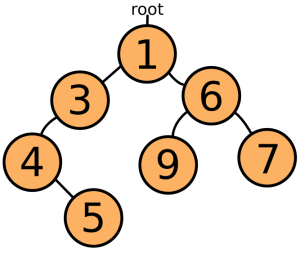
\includegraphics{tree}} 
\smallskip
  
Struktury tego rodzaju nazywa się drzewami\index{drzewo} ze względu na to, jak się rozgałęziają. Teraz gdy potrzebny jest najmniejszy element, wystarczy pobrać pierwszy element i przeorganizować strukturę tak, aby jeden z potomków tego elementu — o najmniejszej wartości — stał się pierwszy. Wstawiając nowe elementy, „przechodzi się” w dół drzewa, aż znajdzie się element mniejszy od nowego i wstawia się go tam. To wymaga o wiele mniej szukania niż w~posortowanej tabeli, ale wadą tego rozwiązania jest utworzenie dużej liczby obiektów, co również ujemnie wpływa na wydajność.


\begin{center} 
 • • • • • 
 \end{center}

  
W kopcu binarnym wykorzystuje się posortowaną tablicę, ale jest ona tylko częściowo posortowana, podobnie jak w powyższym drzewie. Zamiast z~obiektów, drzewo jest zbudowane z pozycji w tablicy, co usiłowałem pokazać na poniższym rysunku:

\bigskip 
 \centerline{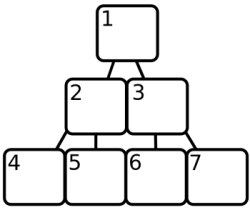
\includegraphics{heap}} 
 \smallskip
  
Element tablicy \texttt{1} jest korzeniem drzewa, elementy \texttt{2} i \texttt{3} są jego dziećmi i ogólnie rzecz biorąc element \texttt{X} ma dzieci \texttt{X * 2} oraz \texttt{X * 2 + 1}. Rozumiesz teraz, dlaczego strukturę tę nazwano kopcem? Zwróć uwagę, że indeksowanie w tej tablicy rozpoczyna się od \texttt{1}, podczas gdy w języku JavaScript indeksy tablicy zaczynają się od \texttt{0}. W kopcu najmniejszy element zawsze znajduje się na pozycji \texttt{1}, a da każdego elementu w tablicy na pozycji \texttt{X}, element na pozycji \texttt{X / 2} (zaokrąglamy w dół) jest mniejszy.

  
Zatem znalezienie najmniejszego elementu wymaga tylko pobrania elementu znajdującego się na pozycji \texttt{1}. Kiedy jednak element ten zostanie pobrany, kopiec musi pozbyć się wszelkich dziur powstałych w tablicy. W tym celu pobiera ostatni element tablicy i przenosi go na początek, a następnie porównuje go z elementami potomnymi na pozycjach \texttt{2} i \texttt{3}. Jest spore prawdopodobieństwo, że będzie większy, a więc zostanie zamieniony miejscami z~jednym z nich i proces porównywania z dziećmi jest powtarzany dla nowej pozycji i tak w kółko, aż element trafi na pozycję, na której jego dzieci będą od niego większe lub nie będzie miał dzieci.

  \begin{verbatim} 
[2, 3, 5, 4, 8, 7, 6]
Zabierz 2, przenieś 6 na początek.
[6, 3, 5, 4, 8, 7]
6 jest większe od pierwszego dziecka 3, a więc następuje zamiana.
[3, 6, 5, 4, 8, 7]
Teraz 6 ma dzieci 4 i 8 (pozycje 4 i 5). Jest większy od
4, a więc ponownie następuje zamiana.
[3, 4, 5, 6, 8, 7]
6 jest na pozycji 4 i nie ma dzieci. Kopiec jest uporządkowany
.
 \end{verbatim}
  
Analogicznie, gdy do kopca zostaje dodany nowy element, jest on umieszczany na końcu tablicy i „przepychany” w górę poprzez zamienianie miejscami z rodzicami, aż uda się znaleźć rodzica mniejszego od niego.

  \begin{verbatim} 
[3, 4, 5, 6, 8, 7]
Element 2 zostaje dodany z powrotem, na końcu.
[3, 4, 5, 6, 8, 7, 2]
2 znajduje się na pozycji 7, a jej rodzic znajduje się na pozycji 3 
i jest to 5. 5 jest większa od 2, a więc następuje zamiana.
[3, 4, 2, 6, 8, 7, 5]
Rodzicem pozycji 3 jest pozycja 1. Znowu zamieniamy.
[2, 4, 3, 6, 8, 7, 5]
Elementu nie da się przesłać dalej, a więc kończymy.
 \end{verbatim}
  
Zwróć uwagę, że aby dodać element nie trzeba go porównywać z każdym elementem tablicy. W istocie z uwagi na fakt, że skoki między rodzicami i~dziećmi są większe im większa jest tablica, zaleta ta jest szczególnie duża, gdy elementów jest dużo\footnote{Liczbę potrzebnych operacji porównywania — w najgorszym przypadku — można wyznaczyć jako logarytm (o podstawie 2) z liczby elementów kopca.}.


\begin{center} 
 • • • • • 
 \end{center}

  
Poniżej znajduje się kod implementacji kopca binarnego. Dwie rzeczy na które warto zwrócić uwagę to to, że zamiast bezpośrednio porównywać elementy wstawiane do kopca najpierw wywoływana jest na nich funkcja \texttt{scoreFunction}, co sprawia, że można przechowywać obiekty, których nie można bezpośrednio porównywać.

  
Dodatkowo, jako że w JavaScripcie tablice zaczynają się od \texttt{0}, a w obliczeniach rodzic-dziecko używany jest system zaczynający liczenie od \texttt{1}, w~kodzie znajduje się kilka dziwnie wyglądających obliczeń mających na celu zniwelowanie tych różnic.

\begin{verbatim} 
function BinaryHeap(scoreFunction){
  this.content = [];
  this.scoreFunction = scoreFunction;
}

BinaryHeap.prototype = {
  push: function(element) {
    // Dodanie nowego elementu na końcu tablicy.
    this.content.push(element);
    // Pozwalamy mu „przechodzić” w górę.
    this.bubbleUp(this.content.length - 1);
  },

  pop: function() {
    // Zapisanie pierwszego elementu, aby móc go potem zwrócić.
    var result = this.content[0];
    // Pobranie elementu z końca tablicy.
    var end = this.content.pop();
    // Jeśli pozostały jeszcze jakieś elementy, umieszczamy ostatni element na
    // początku i pozwalamy mu „przesiąknąć” w dół.
    if (this.content.length > 0) {
      this.content[0] = end;
      this.sinkDown(0);
    }
    return result;
  },

  remove: function(node) {
    var len = this.content.length;
    // Aby usunąć wartość, trzeba przeszukać tablicę, aby ją
    // znaleźć.
    for (var i = 0; i < len; i++) {
      if (this.content[i] == node) {
        // Gdy wartość zostanie znaleziona, powtarzany jest proces z „pop”, aby
        // zapełnić lukę.
        var end = this.content.pop();
        if (i != len - 1) {
          this.content[i] = end;
          if (this.scoreFunction(end) < this.scoreFunction(node))
            this.bubbleUp(i);
          else
            this.sinkDown(i);
        }
        return;
      }
    }
    throw new Error("Nie znaleziono węzła.");
  },

  size: function() {
    return this.content.length;
  },

  bubbleUp: function(n) {
    // Pobranie elementu, który ma zostać przeniesiony.
    var element = this.content[n];
    // Jeśli pozycja 0, element nie może „iść” dalej.
    while (n > 0) {
      // Obliczenie indeksu elementu nadrzędnego i pobranie go.
      var parentN = Math.floor((n + 1) / 2) - 1,
          parent = this.content[parentN];
      // Jeśli rodzic jest większy, elementy należy zamienić miejscami.
      if (this.scoreFunction(element) < this.scoreFunction(parent)) {
        this.content[parentN] = element;
        this.content[n] = parent;
        // Aktualizacja „n„, aby kontynuować od nowej pozycji.
        n = parentN;
      }
      // Znaleziono rodzica, który jest mniejszy, a więc nie trzeba iść dalej.
      else {
        break;
      }
    }
  },

  sinkDown: function(n) {
    // Wyszukanie elementu docelowego i jego wartości.
    var length = this.content.length,
        element = this.content[n],
        elemScore = this.scoreFunction(element);

    while(true) {
      // Obliczenie indeksów elementów potomnych.
      var child2N = (n + 1) * 2, child1N = child2N - 1;
      // To służy do zapisania nowej pozycji elementu,
      // jeśli taka jest.
      var swap = null;
      // Jeśli pierwsze dziecko istnieje (znajduje się w tablicy)...
      if (child1N < length) {
        // Wyszukanie go o obliczenie jego wartości.
        var child1 = this.content[child1N],
            child1Score = this.scoreFunction(child1);
        // Jeśli wartość ta jest mniejsza od naszego elementu, musimy dokonać zamiany.
        if (child1Score < elemScore)
          swap = child1N;
      }
      // Wykonanie tych samych testów dla drugiego dziecka.
      if (child2N < length) {
        var child2 = this.content[child2N],
            child2Score = this.scoreFunction(child2);
        if (child2Score < (swap == null ? elemScore : child1Score))
          swap = child2N;
      }

      // Jeśli element trzeba przenieść, zamieniamy go i kontynuujemy.
      if (swap != null) {
        this.content[n] = this.content[swap];
        this.content[swap] = element;
        n = swap;
      }
      // W przeciwnym razie zakończyliśmy pracę.
      else {
        break;
      }
    }
  }
};
\end{verbatim}
  
I prosty test…

 \begin{verbatim} 
var heap = new BinaryHeap(function(x){return x;});
forEach([10, 3, 4, 8, 2, 9, 7, 1, 2, 6, 5],
        method(heap, "push"));

heap.remove(2);
while (heap.size() > 0)
  print(heap.pop());
\end{verbatim}

\chapter{Rozwiązania}


\section*{Rozdział 2}
\label{sol:2}

\subsection*{Ćwiczenie 2.1}
\label{sol:2.1}

Wynikiem tego wyrażenia jest \texttt{true}. Można je rozłożyć na czynniki:

\begin{verbatim} 
(false || true) && !(false && true)
\end{verbatim}

\begin{verbatim} 
true && !false
\end{verbatim}

\begin{verbatim} 
true
\end{verbatim}
      
Mam nadzieję, że zauważyłeś, że wyrażenie \texttt{"zielona" != "trawa"} jest prawdziwe. Oczywiście trawa może być zielona, ale to są dwa różne słowa.

\subsection*{Ćwiczenie 2.2}
\label{sol:2.2}

\begin{verbatim} 
var wynik = 1;
var licznik = 0;
while (licznik < 10) {
  wynik = wynik * 2;
  licznik = licznik + 1;
}
show(wynik);
\end{verbatim}
      
Licznik równie dobrze mógłby mieć wartość początkową \texttt{1} i wówczas test wyglądałby tak: \texttt{<= 10}. Jednak są powody, które poznasz później, aby przyzwyczaić się do liczenia od zera.

      
Oczywiście Twoje rozwiązanie nie musi być identyczne z moim. Powinno tylko działać. Jeśli Twoje rozwiązanie różni się od mojego, postaraj się dokładnie zrozumieć także mój kod.

\subsection*{Ćwiczenie 2.3}
\label{sol:2.3}

\begin{verbatim} 
var linia = "";
var licznik = 0;
while (licznik < 10) {
  linia = linia + "#";
  print(linia);
  licznik = licznik + 1;
}
\end{verbatim}

\subsection*{Ćwiczenie 2.4}
\label{sol:2.4}

\begin{verbatim} 
var wynik = 1;
for (var licznik = 0; licznik < 10; licznik = licznik + 1)
  wynik = wynik * 2;
show(wynik);
\end{verbatim}
      
Zwróć uwagę, że nawet mimo braku znaku \texttt{\{} oznaczającego początek bloku, instrukcja w pętli i tak została wcięta, aby było jasne, że należy do wiersza kodu znajdującego się nad nią.

      
\begin{verbatim} 
var linia = "";
for (var licznik = 0; licznik < 10; licznik = licznik + 1) {
  linia = linia + "#";
  print(linia);
}
\end{verbatim}

\subsection*{Ćwiczenie 2.5}
\label{sol:2.5}

\begin{verbatim} 
var odpowiedz = prompt("Hej, Ty! Ile wynosi 2 + 2?", "");
if (odpowiedz == "4")
  alert("Jesteś genialny.");
else if (odpowiedz == "3" || odpowiedz == "5")
  alert("Prawie!");
else
  alert("Żal mi Ciebie.");
\end{verbatim}

\subsection*{Ćwiczenie 2.6}
\label{sol:2.6}

\begin{verbatim} 
var odpowiedz;
while (true) {
  odpowiedz = prompt("Hej, Ty! Ile wynosi 2 + 2?", "");
  if (odpowiedz == "4") {
    alert("Jesteś genialny.");
    break;
  }
  else if (odpowiedz == "3" || odpowiedz == "5") {
    alert("Prawie!");
  }
  else {
    alert("Żal mi Ciebie.");
  }
}
\end{verbatim}
      
Ponieważ treść pierwszej instrukcji \texttt{if} zawiera teraz dwie instrukcje, dodałem klamry. Jest to kwestia gustu. Łańcuchy instrukcji \texttt{if}/\texttt{else}, w których niektóre klauzule zawierają bloki, a inne pojedyncze instrukcje jak dla mnie wyglądają dziwnie, ale może Ty będziesz miał inne zdanie na ten temat.

Oto inne rozwiązanie, bez użycia instrukcji \texttt{break} i może trochę bardziej eleganckie:
      
\begin{verbatim} 
var wartosc = null;
while (wartosc != "4") {
  wartosc = prompt("Hej, Ty! Ile wynosi 2 + 2?", "");
  if (wartosc == "4")
    alert("Jesteś genialny.");
  else if (wartosc == "3" || wartosc == "5")
    alert("Prawie!");
  else
    alert("Żal mi Ciebie.");
}
\end{verbatim}


\section*{Rozdział 3}
\label{sol:3}

\subsection*{Ćwiczenie 3.1}
\label{sol:3.1}
      
\begin{verbatim} 
function absolute(number) {
  if (number < 0)
    return -number;
  else
    return number;
}

show(absolute(-144));
\end{verbatim}
    
\subsection*{Ćwiczenie 3.2}
\label{sol:3.2}
     
\begin{verbatim} 
function greaterThan(x) {
  return function(y) {
    return y > x;
  };
}

var greaterThanTen = greaterThan(10);
show(greaterThanTen(9));
 \end{verbatim}
 

\section*{Rozdział 4}
\label{sol:4}
    
\subsection*{Ćwiczenie 4.1}
\label{sol:4.1}

Zadanie to można wykonać zapisując zawartość zbioru jako własności obiektu. Dodawanie imion polegałoby na zdefiniowaniu własności o takich nazwach i dowolnych wartościach. Usuwanie imion polegałoby na kasowaniu odpowiadających im własności. Za pomocą operatora \texttt{in} można natomiast sprawdzać, czy wybrane imię znajduje się już w zbiorze \footnote{Podejście to ma kilka subtelnych wad, które zostaną omówione w \hyperref[chap:8]{rozdziale 8}. W~tym rozdziale wystarczy to, co jest.}.
      
\begin{verbatim} 
var set = {"Spot": true};
// Dodanie White Fang do zbioru
set["White Fang"] = true;
// Usunięcie Spot
delete set["Spot"];
// Sprawdzenie czy "Asoka" znajduje się w zbiorze
show("Asoka" in set);
 \end{verbatim}
    
  
\subsection*{Ćwiczenie 4.2}
\label{sol:4.2}
      
\begin{verbatim} 
function range(upto) {
  var result = [];
  for (var i = 0; i <= upto; i++)
    result[i] = i;
  return result;
}
show(range(4));
 \end{verbatim}
      
Zamiast zmienną pętlową nazywać \texttt{counter} albo \texttt{current}, jak było do tej pory, tym razem nadałem jej nazwę \texttt{i}. Stosowanie jednoliterowych nazw, zazwyczaj \texttt{i}, \texttt{j} lub \texttt{k}, dla zmiennych pętlowych jest szeroko przyjętym zwyczajem wśród programistów. Źródeł jego powstania należy upatrywać przede wszystkim w lenistwie: każdy woli wpisać jedną literę zamiast siedmiu, a~nazwy typu \texttt{counter} albo \texttt{current} i tak niewiele wyjaśniają, do czego dana zmienna służy.

      
Jeśli jednak w programie znajdzie się zbyt dużo jednoliterowych nazw zmiennych, to zrozumienie sposobu jego działania może stać się strasznie trudne. We własnych programach staram się tak krótkich nazw używać tylko w kilku typowych przypadkach. Należą do nich także niezbyt rozbudowane pętle. Jeśli pętla zawiera inną pętlę, która również ma zmienną o nazwie \texttt{i}, wewnętrzna pętla zmodyfikuje zmienną używaną przez zewnętrzną pętlę i nastąpi wielka awaria. W wewnętrznej pętli można by było zatem użyć nazwy \texttt{j}, ale ogólnie rzecz biorąc przyjmuje się, że jeśli pętla jest rozbudowana, powinno się użyć jakiejś znaczącej nazwy zmiennej, aby łatwiej było zrozumieć sposób działania całej konstrukcji.


\subsection*{Ćwiczenie 4.3}
\label{sol:4.3}
         
\begin{verbatim} 
var array = ["a", "b", "c d"];
show(array.join(" ").split(" "));
\end{verbatim}
   

\subsection*{Ćwiczenie 4.4}
\label{sol:4.4}
 
\begin{verbatim} 
function startsWith(string, pattern) {
  return string.slice(0, pattern.length) == pattern;
}

show(startsWith("rotacja", "rot"));
\end{verbatim}


\subsection*{Ćwiczenie 4.5}
\label{sol:4.5}

\begin{verbatim} 
function catNames(paragraph) {
  var colon = paragraph.indexOf(":");
  return paragraph.slice(colon + 2).split(", ");
}

show(catNames("urodzeni 20/09/2004 (matka Yellow Bess): " +
              "Doctor Hobbles 2, Noog"));
\end{verbatim}
      
Najtrudniejsza część, która w pierwotnym opisie algorytmu została pominięta to obsługa spacji znajdujących się za dwukropkiem i przecinków. Wyrażenie \texttt{+ 2} użyte w instrukcji tnącej łańcuch jest potrzebne po to, aby pominąć dwukropek i znajdującą się za nim spację. Argument metody \texttt{split} zawiera zarówno przecinek jak i spację, ponieważ imiona normalnie rozdziela się właśnie za pomocą przecinków i spacji, a nie samych przecinków.

      
Ta funkcja nie wykonuje żadnych testów w celu wykrycia potencjalnych problemów. Założyliśmy, że dane wejściowe będą zawsze poprawne.

    
\subsection*{Ćwiczenie 4.6}
\label{sol:4.6}
      
\begin{verbatim} 
function extractDate(paragraph) {
  function numberAt(start, length) {
    return Number(paragraph.slice(start, start + length));
  }
  return new Date(numberAt(14, 4), numberAt(11, 2) - 1,
                  numberAt(8, 2));
}

show(extractDate("odeszli 27-04-2006: Black Leclère"));
 \end{verbatim}
      
Wywołań funkcji \texttt{Number} można by było się pozbyć, ale jak pisałem wcześniej, wolę unikać używania łańcuchów jako liczb. Funkcja wewnętrzna została utworzona po to, aby nie musieć powtarzać wywołań \texttt{Number} i \texttt{slice} trzy razy.

      
Zwróć uwagę na wartość \texttt{- 1} użytą jako numer miesiąca. Ciotka Emilia, jak większość ludzi liczy miesiące od 1, a więc musimy dostosować tę wartość przed dodaniem jej do konstruktora obiektu \texttt{Date}. (W przypadku numeru dnia ten problem nie występuje, ponieważ dni w obiekcie \texttt{Date} są liczone w~„ludzki” sposób.)

      
W \hyperref[chap:10]{rozdziale 10} poznasz bardziej praktyczne i niezawodne sposoby wydobywania fragmentów z łańcuchów o ustalonej strukturze.

    
\subsection*{Ćwiczenie 4.7}
\label{sol:4.7}   
 
\begin{verbatim} 
function between(string, start, end) {
  var startAt = string.indexOf(start) + start.length;
  var endAt = string.indexOf(end, startAt);
  return string.slice(startAt, endAt);
}
show(between("bu ] boo [ bah ] gzz", "[ ", " ]"));
 \end{verbatim}
    

\subsection*{Ćwiczenie 4.8}
\label{sol:4.8}

\begin{verbatim} 
function formatDate(date) {
  function pad(number) {
    if (number < 10)
      return "0" + number;
    else
      return number;
  }
  return pad(date.getDate()) + "." + pad(date.getMonth() + 1) +
             "." + date.getFullYear();
}
print(formatDate(new Date(2000, 0, 1)));
 \end{verbatim}


\subsection*{Ćwiczenie 4.9}
\label{sol:4.9}

\begin{verbatim} 
function oldestCat(data) {
  var oldest = null;

  for (var name in data) {
    var cat = data[name];
    if (!("death" in cat) &&

        (oldest == null || oldest.birth > cat.birth))
      oldest = cat;
  }

  if (oldest == null)
    return null;
  else
    return oldest.name;
}

print(oldestCat(catData));
 \end{verbatim}
      
Warunek w instrukcji \texttt{if} może się wydawać bardzo skomplikowany. Można go przeczytać tak: „bieżącego kota zapisz w zmiennej \texttt{oldest} tylko, jeśli nie jest martwy i zmienna \texttt{oldest} ma wartość \texttt{null} albo zawiera kota, który urodził się później niż bieżący kot”.
      
Zauważ, że funkcja ta zwraca wartość \texttt{null}, jeśli w \texttt{data} nie ma żyjących kotów. Co Twoje rozwiązanie robi w tym przypadku?


\subsection*{Ćwiczenie 4.10}
\label{sol:4.10}
      
\begin{verbatim} 
function range(start, end) {
  if (arguments.length < 2) {
    end = start;
    start = 0;
  }
  var result = [];
  for (var i = start; i <= end; i++)
    result.push(i);
  return result;
}

show(range(4));
show(range(2, 4));
\end{verbatim}
      
Opcjonalny argument w tej funkcji nie działa dokładnie tak samo, jak w funkcji \texttt{add} w przykładzie powyżej. Gdy nie zostanie podany, jego rolę przejmuje pierwszy argument, a argument \texttt{start} otrzymuje wartość \texttt{0}.


\subsection*{Ćwiczenie 4.11}
\label{sol:4.11}

\begin{verbatim} 
function sum(numbers) {
  var total = 0;
  for (var i = 0; i < numbers.length; i++)
    total += numbers[i];
  return total;
}

print(sum(range(1, 10)));
\end{verbatim}


\section*{Rozdział 6}
\label{sol:6}
  
\subsection*{Ćwiczenie 6.1}
\label{sol:6.1}
    
\begin{verbatim} 
function countZeroes(array) {
  function counter(total, element) {
    return total + (element === 0 ? 1 : 0);
  }
  return reduce(counter, 0, array);
}
 \end{verbatim}
    
\index{?:}Ten dziwny fragment ze znakiem zapytania to nowy operator. W \hyperref[chap:2]{rozdziale 2} poznałeś operatory jedno- i dwuargumentowe. Ten natomiast jest trójargumentowy, tzn. działa na trzech wartościach. Efekt jego działania jest podobny do instrukcji \texttt{if}/\texttt{else}, z tym, że instrukcja \texttt{if} warunkowo wykonuje instrukcje, a ten operator warunkowo wybiera wyrażenia. Pierwszy argument, znajdujący się przed znakiem zapytania, jest warunkiem. Jeśli wartością warunku jest \texttt{true}, wybrane zostaje wyrażenie znajdujące się bezpośrednio za znakiem zapytania — w tym przypadku \texttt{1}. Jeśli jest \texttt{false}, wybrana zostaje część znajdująca się za dwukropkiem — w tym przypadku \texttt{0}.

    
Dzięki temu operatorowi można znacznie skrócić niektóre fragmenty kodu. Gdy jednak wyrażenia są bardzo duże albo w warunkach trzeba podjąć więcej decyzji, to zazwyczaj zwykłe instrukcje \texttt{if} i \texttt{else} są bardziej przejrzyste.

    
Poniżej znajduje się rozwiązanie z użyciem funkcji \texttt{count} z funkcją tworzącą testery równości, dzięki której ostateczna funkcja \texttt{countZeroes} może być jeszcze krótsza:

    
\begin{verbatim} 
function count(test, array) {
  return reduce(function(total, element) {
    return total + (test(element) ? 1 : 0);
  }, 0, array);
}

function equals(x) {
  return function(element) {return x === element;};
}

function countZeroes(array) {
  return count(equals(0), array);
}
\end{verbatim}

  
\subsection*{Ćwiczenie 6.2}
\label{sol:6.2}
    
\begin{verbatim} 
function processParagraph(paragraph) {
  var header = 0;
  while (paragraph.charAt(0) == "%") {
    paragraph = paragraph.slice(1);
    header++;
  }

  return {type: (header == 0 ? "p" : "h" + header),
          content: paragraph};
}

show(processParagraph(paragraphs[0]));
// → {type: "h1", content: " Księga programowania"}
\end{verbatim}

  
\subsection*{Ćwiczenie 6.3}
\label{sol:6.3}
  
  
    
Oto jedno z możliwych rozwiązań tego problemu:

    
\begin{verbatim} 
function splitParagraph(text) {
  function indexOrEnd(character) {
    var index = text.indexOf(character);
    return index == -1 ? text.length : index;
  }

  function takeNormal() {
    var end = reduce(Math.min, text.length,
                     map(indexOrEnd, ["*", "{"]));
    var part = text.slice(0, end);
    text = text.slice(end);
    return part;
  }

  function takeUpTo(character) {
    var end = text.indexOf(character, 1);
    if (end == -1)
      throw new Error("Brak zamykającego '" + character + "'");
    var part = text.slice(1, end);
    text = text.slice(end + 1);
    return part;
  }

  var fragments = [];

  while (text != "") {
    if (text.charAt(0) == "*")
      fragments.push({type: "emphasised",
                      content: takeUpTo("*")});
    else if (text.charAt(0) == "{")
      fragments.push({type: "footnote",
                      content: takeUpTo("}")});
    else
      fragments.push({type: "normal",
                      content: takeNormal()});
  }
  return fragments;
}
\end{verbatim}
    
Zwróć uwagę na sposób użycia funkcji \texttt{map} i \texttt{reduce} w funkcji \texttt{takeNormal}. To jest rozdział o programowaniu funkcyjnym, a więc programujemy funkcyjnie! Rozumiesz, jak to działa? Funkcja \texttt{map} zwraca tablicę pozycji, na których znaleziono podane znaki lub koniec łańcucha, jeśli nic nie znaleziono, a funkcja \texttt{reduce} pobiera minimum z nich, które określa następny punkt w łańcuchu do przejrzenia.

    
Gdybyśmy to zapisali bez mapowania i redukowania, otrzymalibyśmy coś takiego:

    
\begin{verbatim} 
var nextAsterisk = text.indexOf("*");
var nextBrace = text.indexOf("{");
var end = text.length;
if (nextAsterisk != -1)
  end = nextAsterisk;
if (nextBrace != -1 && nextBrace < end)
  end = nextBrace;
 \end{verbatim}
    
To jest jeszcze brzydsze. W większości przypadków, gdy trzeba dokonać decyzji na podstawie szeregu warunków, nawet jeśli są tylko dwa, użycie operacji tablicowych jest bardziej eleganckim rozwiązaniem niż obsługa każdej wartości w osobnej instrukcji \texttt{if}. (W \hyperref[chap:10]{rozdziale 10} jest opisany lepszy sposób na znajdowanie pierwszego wystąpienia „tego lub tamtego znaku” w~łańcuchu.)

    
Jeśli Twoja funkcja \texttt{splitParagraph} zapisuje fragmenty w inny sposób niż w powyższym rozwiązaniu, może być konieczne jej zmodyfikowanie, ponieważ funkcje przedstawione w dalszej części tego rozdziału wymagają, aby fragmenty były obiektami mającymi własności \texttt{type} i \texttt{content}.

  
\subsection*{Ćwiczenie 6.4}
\label{sol:6.4}
    
\begin{verbatim} 
function image(src) {
  return tag("img", [], {src: src});
}
 \end{verbatim}

  
\subsection*{Ćwiczenie 6.5}
\label{sol:6.5}
    
\begin{verbatim} 
function renderParagraph(paragraph) {
  return tag(paragraph.type, map(renderFragment,
                                 paragraph.content));
}

function renderFragment(fragment) {
  if (fragment.type == "reference")
    return footnote(fragment.number);
  else if (fragment.type == "emphasised")
    return tag("em", [fragment.content]);
  else if (fragment.type == "normal")
    return fragment.content;
}
\end{verbatim}

\section*{Rozdział 7}
\label{sol:7}

\subsection*{Ćwiczenie 7.1}
\label{sol:7.1}
    
\begin{verbatim} 
function makeRoads(start) {
  for (var i = 1; i < arguments.length; i += 2)
    makeRoad(start, arguments[i], arguments[i + 1]);
}
\end{verbatim}
    
Funkcja ta ma jeden nazwany parametr o nazwie \texttt{start}, a pozostałe pobiera z quasi-tablicy \texttt{arguments}. Zmienna \texttt{i} ma początkową wartość \texttt{1}, ponieważ musi pominąć pierwszy parametr. Przypomnę też, że zapis \texttt{i += 2} jest skróconą formą konstrukcji \texttt{i = i + 2}.
    
\begin{verbatim} 
var roads = {};
makeRoads("Point Kiukiu", "Hanaiapa", 19,
          "Mt Feani", 15, "Taaoa", 15);
makeRoads("Airport", "Hanaiapa", 6, "Mt Feani", 5,
          "Atuona", 4, "Mt Ootua", 11);
makeRoads("Mt Temetiu", "Mt Feani", 8, "Taaoa", 4);
makeRoads("Atuona", "Taaoa", 3, "Hanakee pearl lodge", 1);
makeRoads("Cemetery", "Hanakee pearl lodge", 6, "Mt Ootua", 5);
makeRoads("Hanapaoa", "Mt Ootua", 3);
makeRoads("Puamua", "Mt Ootua", 13, "Point Teohotepapapa", 14);

show(roads["Airport"]);
\end{verbatim}

  
\subsection*{Ćwiczenie 7.2}
\label{sol:7.2}
    
\begin{verbatim} 
function filter(test, array) {
  var result = [];
  forEach(array, function (element) {
    if (test(element))
      result.push(element);
  });
  return result;
}

show(filter(partial(op[">"], 5), [0, 4, 8, 12]));
 \end{verbatim}
    
(Jeśli wynik tego zastosowania funkcji \texttt{filter} zaskoczył Cię, pamiętaj że argument podany do funkcji \texttt{partial} jest używany jako \emph{pierwszy} argument funkcji, a więc zostaje użyty po lewej stronie operatora \texttt{>}.)

  
\subsection*{Ćwiczenie 7.3}
\label{sol:7.3}
    
\begin{verbatim} 
function shortestRoute(from, to) {
  var currentShortest = null;
  forEach(possibleRoutes(from, to), function(route) {
    if (!currentShortest || currentShortest.length > route.length)
      currentShortest = route;
  });
  return currentShortest;
}
\end{verbatim}
    
Sztuka w „minimalizowaniu” i „maksymalizowaniu” algorytmów polega na tym, aby niczego nie zepsuć, gdy otrzyma się pustą tablicę. W tym przypadku wiemy, że każde dwa miejsca łączy przynajmniej jedna droga, a więc możemy ten problem zignorować. Ale byłoby to nieprofesjonalne. Co się stanie, gdy droga z Puamua do Mount Ootua, która jest stroma i błotnista, zostanie zmieciona z powierzchni przez lawinę błotną? Byłoby wstyd, gdyby miało to unieruchomić naszą funkcję i dlatego gdy żadne trasy nie zostaną znalezione, zwracamy \texttt{null}.

    
Poniżej przedstawione jest funkcyjne podejście z abstrakcją wszystkiego, co się dało:

    
\begin{verbatim} 
function minimise(func, array) {
  var minScore = null;
  var found = null;
  forEach(array, function(element) {
    var score = func(element);
    if (minScore == null || score < minScore) {
      minScore = score;
      found = element;
    }
  });
  return found;
}

function getProperty(propName) {
  return function(object) {
    return object[propName];
  };
}

function shortestRoute(from, to) {
  return minimise(getProperty("length"), possibleRoutes(from, to));
}
\end{verbatim}
    
Niestety ta wersja jest trzy razy dłuższa od poprzedniej. W programach, w~których trzeba coś zminimalizować dobrym pomysłem jest napisanie ogólnego algorytmu, aby można go było użyć wielokrotnie. W większości przypadków pierwsza wersja powinna być wystarczająco dobra.

    
Zwróć jednak uwagę na funkcję \texttt{getProperty}\index{getProperty}, która jest często przydatna przy programowaniu funkcyjnym z użyciem obiektów.


\subsection*{Ćwiczenie 7.4}
\label{sol:7.4}
    
\begin{verbatim} 
function possibleDirections(from) {
  var mapSize = 20;
  function insideMap(point) {
    return point.x >= 0 && point.x < mapSize &&
           point.y >= 0 && point.y < mapSize;
  }

  var directions = [point(-1, 0), point(1, 0), point(0, -1),
                    point(0, 1), point(-1, -1), point(-1, 1),
                    point(1, 1), point(1, -1)];
  return filter(insideMap, map(partial(addPoints, from),
                               directions));
}

show(possibleDirections(point(0, 0)));
\end{verbatim}
    
Zmienną \texttt{mapSize} utworzyłem tylko po to, aby nie musieć wpisywać \texttt{20} dwa razy. Gdybyśmy za jakiś czas chcieli użyć tej funkcji na innej mapie, jej kod wyglądałby niezgrabnie z tymi wszystkimi \texttt{20}, które trzeba by było pozmieniać. Moglibyśmy nawet funkcji \texttt{mapSize} użyć jako argumentu funkcji \texttt{possibleDirections}, dzięki czemu moglibyśmy jej używać na innych mapach bez zmieniania czegokolwiek. Uznałem jednak, że tutaj nie jest to konieczne, a w razie potrzeby zawsze można to zmienić.

    
Dlaczego w takim razie nie utworzyłem zmiennej do przechowywania wartości \texttt{0}, która również występuje dwa razy? Przyjmuję założenie, że mapy zawsze zaczynają się od \texttt{0} i jest mało prawdopodobne, żeby wartość ta miała się zmienić, a dodatkowa zmienna powoduje tylko więcej bałaganu.

  
\subsection*{Ćwiczenie 7.5}
\label{sol:7.5}
    
\begin{verbatim} 
function estimatedDistance(pointA, pointB) {
  var dx = Math.abs(pointA.x - pointB.x),
      dy = Math.abs(pointA.y - pointB.y);
  if (dx > dy)
    return (dx - dy) * 100 + dy * 141;
  else
    return (dy - dx) * 100 + dx * 141;
}
 \end{verbatim}
    
Te dziwne wzory służą do rozłożenia ścieżki na część prostą i skośną. Spójrz na poniższą przykładową ścieżkę.

\bigskip 
\centerline{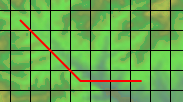
\includegraphics{diagonalpath}} 
\smallskip
    
Ścieżka ta ma \texttt{6} kwadratów szerokości i \texttt{3} kwadraty wysokości, a więc wykonujemy \texttt{6 - 3 = 3} prostych ruchów i \texttt{3} skośne.

    
Moglibyśmy odległość między dwoma punktami obliczać przy użyciu funkcji implementującej twierdzenie Pitagorasa. Potrzebujemy optymistycznego szacunku, a przyjęcie założenia, że można iść prosto do celu na pewno jest optymistyczne. Jednak im szacunek jest bliższy rzeczywistej odległości, tym mniej bezużytecznych ścieżek program musi sprawdzić.

  
\subsection*{Ćwiczenie 7.6}
\label{sol:7.6}
    
Jednym z dobrych pomysłów może być użycie obiektu zawierającego obiekty. Jedna ze współrzędnych punktów, np. \texttt{x}, jest używana jako nazwa własności dla zewnętrznego obiektu, a druga, \texttt{y}, dla obiektu wewnętrznego. To wymaga jednak prowadzenia zapisów, ponieważ czasami szukany obiekt wewnętrzny jeszcze nie będzie istniał.
    
\begin{verbatim} 
function makeReachedList() {
  return {};
}

function storeReached(list, point, route) {
  var inner = list[point.x];
  if (inner == undefined) {
    inner = {};
    list[point.x] = inner;
  }
  inner[point.y] = route;
}

function findReached(list, point) {
  var inner = list[point.x];
  if (inner == undefined)
    return undefined;
  else
    return inner[point.y];
}
\end{verbatim}
    
Inną możliwością jest połączenie współrzędnych \texttt{x} i \texttt{y} punktu w jedną nazwę własności i użycie jej do przechowywania tras w pojedynczym obiekcie.
    
\begin{verbatim} 
function pointID(point) {
  return point.x + "-" + point.y;
}

function makeReachedList() {
  return {};
}

function storeReached(list, point, route) {
  list[pointID(point)] = route;
}

function findReached(list, point) {
  return list[pointID(point)];
}
\end{verbatim}

\section*{Rozdział 8}
\label{sol:8}

\subsection*{Ćwiczenie 8.1}
\label{sol:8.1}
    
\begin{verbatim} 
function Point(x, y) {
  this.x = x;
  this.y = y;
}
Point.prototype.add = function(other) {
  return new Point(this.x + other.x, this.y + other.y);
};
Point.prototype.isEqualTo = function(other) {
  return this.x == other.x && this.y == other.y;
};

show((new Point(3, 1)).add(new Point(2, 4)));
\end{verbatim}
    
Pamiętaj, aby Twoja wersja metody \texttt{add} pozostawiała punkt \texttt{this} nietknięty i tworzyła nowy obiekt. Metoda zmieniająca bieżący obiekt działałaby podobnie do operatora \texttt{+=}, który z kolei działa jak operator \texttt{+}.

  
\subsection*{Ćwiczenie 8.2}
\label{sol:8.2}
    
\begin{verbatim} 
Grid.prototype.each = function(action) {
  for (var y = 0; y < this.height; y++) {
    for (var x = 0; x < this.width; x++) {
      var point = new Point(x, y);
      action(point, this.valueAt(point));
    }
  }
};
\end{verbatim}
  
 
\subsection*{Ćwiczenie 8.3}
\label{sol:8.3}
    
\begin{verbatim} 
Terrarium.prototype.toString = function() {
  var characters = [];
  var endOfLine = this.grid.width - 1;
  this.grid.each(function(point, value) {
    characters.push(characterFromElement(value));
    if (point.x == endOfLine)
      characters.push("\n");
  });
  return characters.join("");
};
 \end{verbatim}
    
Wypróbuj ten kod…

    
\begin{verbatim} 
var terrarium = new Terrarium(thePlan);
print(terrarium.toString());
// → ############################
//   #      #    #      o      ##
//   #                          #
//   #          #####           #
//   ##         #   #    ##     #
//   ###           ##     #     #
//   #           ###      #     #
//   #   ####                   #
//   #   ##       o             #
//   # o  #         o       ### #
//   #    #                     #
//   ############################
\end{verbatim}

  
\subsection*{Ćwiczenie 8.4}
\label{sol:8.4}
    
Nazwę metody można przekazać jako łańcuch. Dzięki temu funkcja \texttt{method} może sama znaleźć odpowiednią wartość funkcyjną.

    
\begin{verbatim} 
function method(object, name) {
  return function() {
    object[name].apply(object, arguments);
  };
}

var pushTest = method(testArray, "push");
\end{verbatim}

  
\subsection*{Ćwiczenie 8.5}
\label{sol:8.5}
    
\begin{verbatim} 
Terrarium.prototype.listSurroundings = function(center) {
  var result = {};
  var grid = this.grid;
  directions.each(function(name, direction) {
    var place = center.add(direction);
    if (grid.isInside(place))
      result[name] = characterFromElement(grid.valueAt(place));
    else
      result[name] = "#";
  });
  return result;
};
\end{verbatim}
    
Zwróć uwagę na użycie zmiennej \texttt{grid} w celu obejścia problemu z \texttt{this}.

  
\subsection*{Ćwiczenie 8.6}
\label{sol:8.6}
    
Aby wybrać losowy kierunek, potrzebna nam jest tablica nazw kierunków. Oczywiście moglibyśmy po prostu napisać \texttt{["n", "ne", ...]}, ale to oznaczałoby duplikowanie informacji, a powielanie danych mnie złości. Moglibyśmy też do budowy tej tablicy użyć instrukcji \texttt{each} w obiekcie \texttt{directions}, co byłoby już lepszym rozwiązaniem.
    
Jednak w tym przypadku jest możliwość zastosowania uogólnienia. Możliwość utworzenia listy nazw własności znajdujących się w słowniku wydaje się bardzo przydatna, a więc dodamy takie narzędzie do prototypu \texttt{Dictionary}.
    
\begin{verbatim} 
Dictionary.prototype.names = function() {
  var names = [];
  this.each(function(name, value) {names.push(name);});
  return names;
};

show(directions.names());
\end{verbatim}
    
Neurotyk od razu dodałby jeszcze dla równowagi metodę \texttt{values} zwracającą listę wartości zapisanych w słowniku. Myślę jednak, że to może poczekać, aż \href{http://www.c2.com/cgi/wiki?YouArentGonnaNeedIt}{będzie potrzebne}.
    
Oto sposób pobrania losowego elementu z tablicy:
    
\begin{verbatim} 
function randomElement(array) {
  if (array.length == 0)
    throw new Error("Tablica jest pusta.");
  return array[Math.floor(Math.random() * array.length)];
}

show(randomElement(["heads", "tails"]));
 \end{verbatim}
    
A to jest owad we własnej osobie:
    
\begin{verbatim} 
function DrunkBug() {};
DrunkBug.prototype.act = function(surroundings) {
  return {type: "move",
          direction: randomElement(directions.names())};
};
DrunkBug.prototype.character = "~";

creatureTypes.register(DrunkBug);
\end{verbatim}

  
\subsection*{Ćwiczenie 8.7}
\label{sol:8.7}
     
\begin{verbatim} 
function LichenEater() {
  this.energy = 10;
}
LichenEater.prototype.act = function(surroundings) {
  var emptySpace = findDirections(surroundings, " ");
  var lichen = findDirections(surroundings, "*");

  if (this.energy >= 30 && emptySpace.length > 0)
    return {type: "reproduce", direction: randomElement(emptySpace)};
  else if (lichen.length > 0)
    return {type: "eat", direction: randomElement(lichen)};
  else if (emptySpace.length > 0)
    return {type: "move", direction: randomElement(emptySpace)};
  else
    return {type: "wait"};
};
LichenEater.prototype.character = "c";

creatureTypes.register(LichenEater);
\end{verbatim}

  
\subsection*{Ćwiczenie 8.8}
\label{sol:8.8}
    
Jednym z rozwiązań może być rezygnacja z losowego wybierania kierunków ruchu. gdy kierunki są wybierane losowo, stwory często poruszają się w tę i~z~powrotem ostatecznie nigdzie nie docierając. Jeśli stworzenie będzie pamiętać kierunek ostatniego ruchu i preferować jego kontynuację, zmarnuje mniej czasu i szybciej dotrze do pożywienia.

    
\begin{verbatim} 
function CleverLichenEater() {
  this.energy = 10;
  this.direction = "ne";
}
CleverLichenEater.prototype.act = function(surroundings) {
  var emptySpace = findDirections(surroundings, " ");
  var lichen = findDirections(surroundings, "*");

  if (this.energy >= 30 && emptySpace.length > 0) {
    return {type: "reproduce",
            direction: randomElement(emptySpace)};
  }
  else if (lichen.length > 1) {
    return {type: "eat",
            direction: randomElement(lichen)};
  }
  else if (emptySpace.length > 0) {
    if (surroundings[this.direction] != " ")
      this.direction = randomElement(emptySpace);
    return {type: "move",
            direction: this.direction};
  }
  else {
    return {type: "wait"};
  }
};
CleverLichenEater.prototype.character = "c";

creatureTypes.register(CleverLichenEater);
 \end{verbatim}
    
Wypróbuj to na poprzedniej planszy terrarium.

  
\subsection*{Ćwiczenie 8.9}
\label{sol:8.9}
    
Rozwiązanie tego problemu musisz znaleźć sam. Mnie nie udało się znaleźć dobrego sposobu na to, aby zapobiec wyginięciu tych stworzeń natychmiast albo zaraz po wytępieniu wszystkich zjadaczy porostów. Sztuczka ze zjadaniem osobników tylko wtedy, gdy dwa z nich znajdują się obok siebie tutaj nie działa, ponieważ osobniki te się ruszają i trudno napotkać je, gdy są obok siebie. Obiecującym rozwiązaniem jest danie zjadaczom zjadaczy dużo energii, dzięki której mogą przetrwać czas, gdy jest mało zjadaczy porostów oraz powolne rozmnażanie, dzięki czemu zasoby pożywienia nie są zbyt szybko zużywane.

    
Życiem porostów i zjadaczy rządzi pewien cykl — raz jest dużo porostów, co powoduje, że rodzi się dużo zjadaczy, co z kolei powoduje, że robi się mało porostów, z którego to powodu zjadacze zaczynają umierać z głodu, co sprawia że porosty znowu się rozrastają itd. Można też spróbować hibernacji zjadaczy zjadaczy porostów (przy użyciu akcji \texttt{wait}) na pewien czas, gdy nie uda im się znaleźć nic do jedzenia przez kilka kolejek. Dobre efekty może przynieść wybudzanie stworów z hibernacji po odpowiedniej liczbie kolejek albo gdy wyczują w pobliżu jedzenie.

\section*{Rozdział 10}
\label{sol:10}

\subsection*{Ćwiczenie 10.1}
\label{sol:10.1}
    
\begin{verbatim} 
var datePattern = /\d\d\/\d\d\/\d\d\d\d/;
show("urodzeni 15/11/2003 (matka Spot): White Fang".search(datePattern));
\end{verbatim}
 
  
\subsection*{Ćwiczenie 10.2}
\label{sol:10.2}
    
\begin{verbatim} 
var mailAddress = /\b[\w\.-]+@[\w\.-]+\.\w{2,3}\b/;

show(mailAddress.test("kenny@test.net"));
show(mailAddress.test("Wyłsałem mleja na adres kenny@tets.nets, ale nie dźła!"));
show(mailAddress.test("the_giant_sloth@gmail.com"));
 \end{verbatim}
    
Ciągi \texttt{\textbackslash b} na początku i końcu wzorca sprawiają, że drugi łańcuch nie pasuje.

  
\subsection*{Ćwiczenie 10.3}
\label{sol:10.3}
    
\begin{verbatim} 
function extractDate(string) {
  var found = string.match(/(\d\d?)\.(\d\d?)\.(\d{4})/);
  if (found == null)
    throw new Error("Nie znaleziono daty w „" + string + "”.");
  return new Date(Number(found[3]), Number(found[2]) - 1,
                  Number(found[1]));
}

show(extractDate("urodzeni 5.2.2007 (matka Noog): Long-ear Johnson"));
\end{verbatim}
    
Ta wersja jest nieco dłuższa niż poprzednia, ale ma tę zaletę, że sprawdza co robi i złości się, gdy otrzyma bezsensowne dane. Bez wyrażeń regularnych osiągnięcie tego było dużo trudniejsze ― trzeba by było wykonać wielu wywołań funkcji \texttt{indexOf}, aby dowiedzieć się czy liczby zawierają jedną cyfrę czy dwie oraz czy łączniki znajdowały się we właściwych miejscach.

  
\subsection*{Ćwiczenie 10.4}
\label{sol:10.4}
    
\begin{verbatim} 
function escapeHTML(text) {
  var replacements = {"<": "<", ">": ">",
                      "&": "&", "\"": """};
  return text.replace(/[<>&"]/g, function(character) {
    return replacements[character];
  });
}

print(escapeHTML("Tekst preformatowany zapisuje się w elemencie \"<pre>\"."));
\end{verbatim}
    
Obiekt \texttt{replacements} pozwala szybko związać każdy znak z jego encją. Używanie go w ten sposób jest bezpieczne (tzn. nie jest potrzebny żaden obiekt \texttt{Dictionary}), ponieważ jedyne własności, jakie będą używane to te, które zostaną dopasowane przez wyrażenie \texttt{/[<>\&"]/}.

\section*{Rozdział 11}
\label{sol:11}
  
\subsection*{Ćwiczenie 11.1}
\label{sol:11.1}
    
\begin{verbatim} 
function validInfo(form) {
  return form.elements.name.value != "" &&
    /^.+@.+\.\w{2,3}$/.test(form.elements.email.value);
}

show(validInfo(document.forms.userinfo));
\end{verbatim}
    
Gdy zastanawiałeś się nad sprawdzaniem adresu e-mail, przyszło ci do głowy, aby użyć wyrażeń regularnych, prawda?

  
\subsection*{Ćwiczenie 11.2}
\label{sol:11.2}
    
\begin{verbatim} 
userForm.elements.send.onclick = function() {
  if (validInfo(userForm))
    userForm.submit();
  else
    alert("Podaj nazwisko i poprawny adres e-mail!");
};
\end{verbatim}

\section*{Rozdział 12}
\label{sol:12}

\subsection*{Ćwiczenie 12.1}
\label{sol:12.1}
     
\begin{verbatim} 
function asHTML(node) {
  if (isTextNode(node))
    return escapeHTML(node.nodeValue);
  else if (node.childNodes.length == 0)
    return "<" + node.nodeName + "/>";
  else
    return "<" + node.nodeName + ">" +
           map(asHTML, node.childNodes).join("") +
           "</" + node.nodeName + ">";
}

print(asHTML(document.body));
\end{verbatim}

  
\subsection*{Ćwiczenie 12.2}
\label{sol:12.2}
    
\begin{verbatim} 
function removeElement(node) {
  if (node.parentNode)
    node.parentNode.removeChild(node);
}

removeElement(newParagraph);
\end{verbatim}
  
  
\subsection*{Ćwiczenie 12.3}
\label{sol:12.3}
    
\begin{verbatim} 
function makeTable(data, columns) {
  var headRow = dom("TR");
  forEach(columns, function(name) {
    headRow.appendChild(dom("TH", null, name));
  });

  var body = dom("TBODY", null, headRow);
  forEach(data, function(object) {
    var row = dom("TR");
    forEach(columns, function(name) {
      row.appendChild(dom("TD", null, String(object[name])));
    });
    body.appendChild(row);
  });

  return dom("TABLE", null, body);
}

var table = makeTable(document.body.childNodes,
                      ["nodeType", "tagName"]);
document.body.appendChild(table);
\end{verbatim}
    
Nie zapomnij przekonwertować wartości z obiektów na łańcuchy przed ich dodaniem do tabeli ― nasza funkcja \texttt{dom} rozpoznaje tylko łańcuchy i węzły DOM.


\section*{Rozdział 13}
\label{sol:13}
 
\subsection*{Ćwiczenie 13.1}
\label{sol:13.1}   
    
\begin{verbatim} 
function registerEventHandler(node, event, handler) {
  if (typeof node.addEventListener == "function")
    node.addEventListener(event, handler, false);
  else
    node.attachEvent("on" + event, handler);
}

registerEventHandler($("button"), "click",
                     function(){print("Klik (2)");});
\end{verbatim}
    
Nie przestrasz się tej długiej i niezgrabnej nazwy. Później będziemy musieli dodać nowe opakowanie, aby opakować to opakowanie i będzie ono miało krótszą nazwę.

    
Można też test ten wykonać tylko raz i zdefiniować \texttt{registerEventHandler} do przechowywania innej funkcji w zależności od przeglądarki. Takie rozwiązanie jest lepsze pod względem wydajnościowym, ale trochę dziwne.

    
\begin{verbatim} 
if (typeof document.addEventListener == "function")
  var registerEventHandler = function(node, event, handler) {
    node.addEventListener(event, handler, false);
  };
else
  var registerEventHandler = function(node, event, handler) {
    node.attachEvent("on" + event, handler);
  };
\end{verbatim}

  
\subsection*{Ćwiczenie 13.2}
\label{sol:13.2}
 
    
\begin{verbatim} 
Square.moveContent = function(target) {
  target.content = this.content;
  this.content = null;
  target.tableCell.appendChild(this.tableCell.lastChild);
};
Square.clearContent = function() {
  this.content = null;
  removeElement(this.tableCell.lastChild);
};
 \end{verbatim}
  
  
\subsection*{Ćwiczenie 13.3}
\label{sol:13.3}
      
\begin{verbatim} 
SokobanField.move = function(direction) {
  var playerSquare = this.getSquare(this.playerPos);
  var targetPos = this.playerPos.add(direction);
  var targetSquare = this.getSquare(targetPos);

  // Możliwość przesunięcia kamienia
  if (targetSquare.hasBoulder()) {
    var pushTarget = this.getSquare(targetPos.add(direction));
    if (pushTarget.isEmpty()) {
      targetSquare.moveContent(pushTarget);
    }
    else if (pushTarget.isExit()) {
      targetSquare.moveContent(pushTarget);
      pushTarget.clearContent();
      this.bouldersToGo--;
      this.updateScore();
    }
  }
  // Przesuwanie gracza
  if (targetSquare.isEmpty()) {
    playerSquare.moveContent(targetSquare);
    this.playerPos = targetPos;
  }
};
\end{verbatim}
    
Dzięki temu, że najpierw obsługiwany jest ruch kamieni, kod ruchu może działać w taki sam sposób zarówno gdy gracz przesuwa się normalnie, jak i gdy popycha kamień. Zwróć uwagę na sposób zlokalizowania kwadratu za kamieniem poprzez dodanie \texttt{direction} dwa razy do \texttt{playerPos}. Przetestuj ten kod przesuwając się w lewo o dwa kwadraty:
    
\begin{verbatim} 
testField.move(new Point(-1, 0));
testField.move(new Point(-1, 0));
\end{verbatim}
    
Jeśli to zadziałało, to przesunęliśmy kamień w miejsce, z którego nie da się go już ruszyć, a więc lepiej to pole usunąć.
    
\begin{verbatim} 
testField.remove();
\end{verbatim}

  
\subsection*{Ćwiczenie 13.4}
\label{sol:13.4}
    
\begin{verbatim} 
SokobanGame.keyDown = function(event) {
  if (arrowKeyCodes.contains(event.keyCode)) {
    event.stop();
    this.field.move(arrowKeyCodes.lookup(event.keyCode));
    if (this.field.won()) {
      if (this.level < sokobanLevels.length - 1) {
        alert("Doskonale! Przechodzisz do następnego poziomu.");
        this.level++;
        this.reset();
      }
      else {
        alert("Wygrałeś! Koniec gry.");
        this.newGame();
      }
    }
  }
};
\end{verbatim}
    
Należy zaznaczyć, że taki sposób przechwytywania zdarzeń klawiszy ― poprzez dodanie procedury do \texttt{document} i zatrzymywanie tych zdarzeń, które nas interesują — nie jest dobrym pomysłem, jeśli w dokumencie znajdują się inne elementy. Spróbuj na przykład przesunąć kursor w polu tekstowym znajdującym się na górze dokumentu. ― Nie uda Ci się to, ponieważ przesuniesz tylko ludzika w grze Sokoban. Gdyby gra miała być używana na prawdziwej stronie internetowej, najlepiej byłoby ją umieścić w ramce lub osobnym oknie, aby przejmowała tylko zdarzenia dotyczące niej.

  
\subsection*{Ćwiczenie 13.5}
\label{sol:13.5}   
    
Czas animacji można kontrolować za pomocą metody \texttt{setInterval}. Pamiętaj,że metoda ta powinna się wyłączyć po wykonaniu swojego zadania. Jeśli tego nie zrobisz, będzie marnowała zasoby komputera dopóki strona nie zostanie zamknięta.

    
\begin{verbatim} 
Square.clearContent = function() {
  self.content = null;
  var image = this.tableCell.lastChild;
  var size = 100;

  var animate = setInterval(function() {
    size -= 10;
    image.style.width = size + "%";
    image.style.height = size + "%";

    if (size < 60) {
      clearInterval(animate);
      removeElement(image);
    }
  }, 70);
};
\end{verbatim}
    
Teraz, jeśli masz kilka godzin możesz spróbować przejść wszystkie poziomy.


\section*{Rozdział 14}
\label{sol:14}

\subsection*{Ćwiczenie 14.1}
\label{sol:14.1}
    
\begin{verbatim} 
function serializeJSON(value) {
  function isArray(value) {
    return /^\s*function Array/.test(String(value.constructor));
  }

  function serializeArray(value) {
    return "[" + map(serializeJSON, value).join(", ") + "]";
  }
  function serializeObject(value) {
    var properties = [];
    forEachIn(value, function(name, value) {
      properties.push(serializeString(name) + ": " +
                      serializeJSON(value));
    });
    return "{" + properties.join(", ") + "}";
  }
  function serializeString(value) {
    var special =
      {"\"": "\\\"", "\\": "\\\\", "\f": "\\f", "\b": "\\b",
       "\n": "\\n", "\t": "\\t", "\r": "\\r", "\v": "\\v"};
    var escaped = value.replace(/[\"\\\f\b\n\t\r\v]/g,
                                function(c) {return special[c];});
    return "\"" + escaped + "\"";
  }

  var type = typeof value;
  if (type == "object" && isArray(value))
    return serializeArray(value);
  else if (type == "object")
    return serializeObject(value);
  else if (type == "string")
    return serializeString(value);
  else
    return String(value);
}

print(serializeJSON(fruit));
\end{verbatim}
    
Sztuczka użyta w funkcji \texttt{serializeString} jest podobna do tego, co zrobiliśmy w funkcji \texttt{escapeHTML} w \hyperref[chap:10]{rozdziale 10}. Zastępnik dla każdego znaku jest znajdowany w obiekcie. Niektóre z nich, jak choćby \texttt{"\textbackslash \textbackslash \textbackslash \textbackslash"}, wyglądają dziwnie, ponieważ każdy ukośnik wsteczny, który ma się pojawić w wyniku musi mieć towarzyszący ukośnik wsteczny.

    
Zwróć też uwagę, że także nazwy własności są zapisane w cudzysłowach, jako łańcuchy. W niektórych przypadkach nie jest to konieczne, ale dla nazw zawierających spacje i jakieś inne dziwne rzeczy tak. Tu zostało użyte uproszczone rozwiązanie polegające na ujęciu w cudzysłów wszystkiego.


\printindex

\end{document}
